\documentclass[11pt,oneside]{book}
\usepackage{fontspec}
\setmainfont{Noto Serif}
\setsansfont{Noto Sans}
\setmonofont{Noto Sans Mono}
\newfontfamily\proseunicodefont{DejaVu Serif}
\usepackage[margin=1in]{geometry}
\usepackage{microtype}
\usepackage{amsmath,amssymb,amsthm,mathtools,bm}
\usepackage{graphicx}
\usepackage{xcolor}
\usepackage{booktabs}
\usepackage{array}
\usepackage{longtable}
\usepackage{enumitem}
\usepackage{float}
\usepackage{caption}
\usepackage{hyperref}
\usepackage{fancyhdr}
\usepackage{tikz}
\usetikzlibrary{arrows.meta,positioning,calc,decorations.pathmorphing}

\hypersetup{
  colorlinks=true,
  linkcolor=blue!50!black,
  urlcolor=blue!50!black,
  citecolor=blue!50!black
}

\setlength{\parskip}{0.5em}
\setlength{\parindent}{0pt}
\setlist[itemize]{topsep=0.25em,itemsep=0.2em}
\setlist[enumerate]{topsep=0.25em,itemsep=0.2em}
\setlength{\headheight}{40pt}
\numberwithin{equation}{chapter}

\newtheorem{theorem}{Satz}[chapter]
\newtheorem{proposition}[theorem]{Proposition}
\newtheorem{lemma}[theorem]{Lemma}
\newtheorem{corollary}[theorem]{Korollar}
\theoremstyle{definition}
\newtheorem{definition}[theorem]{Definition}
\newtheorem{example}[theorem]{Beispiel}
\theoremstyle{remark}
\newtheorem{remark}[theorem]{Bemerkung}

\providecommand{\ket}[1]{\left\lvert#1\right\rangle}
\providecommand{\bra}[1]{\left\langle#1\right\rvert}
\providecommand{\braket}[2]{\left\langle#1\,\middle|\,#2\right\rangle}
\providecommand{\expect}[1]{\left\langle#1\right\rangle}
\newcommand{\lectureoverview}[1]{\paragraph{Überblick.} #1}

\makeatletter
\newcommand{\course@headerfont}{\normalfont\small\itshape}
\newcommand{\course@pagefont}{\normalfont\small}
\newcommand{\course@headerraise}{14pt}
\newlength{\course@headerboxheight}
\setlength{\course@headerboxheight}{\dimexpr\headheight-\course@headerraise-9pt\relax}
\newcommand{\course@leftheadbox}[1]{%
  \raisebox{\course@headerraise}{%
    \parbox[t][\course@headerboxheight][t]{0.82\textwidth}{%
      \raggedright\course@headerfont\strut\MakeUppercase{#1}\strut%
    }%
  }%
}
\newcommand{\course@rightheadbox}[1]{%
  \raisebox{\course@headerraise}{%
    \parbox[t][\course@headerboxheight][t]{0.82\textwidth}{%
      \raggedleft\course@headerfont\strut\MakeUppercase{#1}\strut%
    }%
  }%
}
\renewcommand{\chaptermark}[1]{\markboth{\MakeUppercase{\chaptername\ \thechapter.\ #1}}{}}
\renewcommand{\sectionmark}[1]{\markright{\MakeUppercase{\thesection\hspace{0.4em}#1}}}
\fancyhf{}
\fancyhead[L]{\course@leftheadbox{\leftmark}}
\fancyhead[R]{\course@pagefont\thepage}
\renewcommand{\headrulewidth}{0.5pt}
\pagestyle{fancy}
\fancypagestyle{plain}{%
  \fancyhf{}
  \fancyhead[L]{\course@leftheadbox{\leftmark}}
  \fancyhead[R]{\course@pagefont\thepage}
  \renewcommand{\headrulewidth}{0.5pt}
}
\makeatother

% Video2Book editorial provenance macros
\newenvironment{classroomqa}{%
  \par\medskip\noindent\begin{minipage}{\linewidth}\small\hrule\medskip
}{%
  \medskip\hrule\end{minipage}\par\medskip
}
\newcommand{\audiencequestion}[1]{\noindent\textbf{Frage aus dem Publikum.} #1\par\smallskip}
\newcommand{\lecturerresponse}[1]{\noindent\textbf{Antwort.} #1\par}
\newcommand{\lecturetimestamp}[1]{\footnote{Vorlesungszeit: #1.}}
\newcommand{\lectureframe}[1]{\par\smallskip{\centering\footnotesize\itshape Vorlesungsbild: #1.\par}}
\newcommand{\editorialnote}[1]{\footnote{Redaktionelle Klarstellung: #1}}

\usepackage{polyglossia}
\setdefaultlanguage{german}
\usepackage{sectsty}
\renewcommand{\contentsname}{Inhaltsverzeichnis}
\renewcommand{\chaptername}{Kapitel}
\renewcommand{\figurename}{Abbildung}
\renewcommand{\tablename}{Tabelle}
\renewcommand{\proofname}{Beweis}
\renewcommand{\bibname}{Literatur}
\sectionfont{\raggedright}
\subsectionfont{\raggedright}
\makeatletter
\renewcommand{\@pnumwidth}{2.2em}
\renewcommand{\@tocrmarg}{3.2em}
\makeatother
\usepackage{tocloft}
\renewcommand{\cftchapfont}{\small\bfseries}
\renewcommand{\cftchappagefont}{\small\bfseries}
\renewcommand{\cftsecfont}{\small}
\renewcommand{\cftsecpagefont}{\small}
\setlength{\cftsecnumwidth}{3em}
\renewcommand{\cftsubsecfont}{\small}
\renewcommand{\cftsubsecpagefont}{\small}
\setlength{\cftsubsecindent}{4.5em}
\setlength{\cftsubsecnumwidth}{4em}
\emergencystretch=6em
\pdfstringdefDisableCommands{\def\proseunicodefont{}}

\geometry{paperwidth=177.6mm,paperheight=252mm,left=16mm,right=16mm,
 top=18mm,bottom=18mm,includeheadfoot,headheight=28pt,headsep=7mm,footskip=9mm}
\usepackage{scrextend}
\changefontsizes[17pt]{12pt}
\raggedbottom
\renewenvironment{classroomqa}{\par\medskip\begingroup}{\par\endgroup\medskip}
\fancyhf{}
\setlength{\headwidth}{\textwidth}
\fancyhead[L]{\parbox{\textwidth}{\raggedright\fontsize{9}{11}\selectfont\nouppercase{\leftmark}}}
\fancyfoot[C]{\small\thepage}
\renewcommand{\headrulewidth}{0.3pt}
\fancypagestyle{plain}{\fancyhf{}\fancyfoot[C]{\small\thepage}\renewcommand{\headrulewidth}{0pt}}

\graphicspath{{../../../generated_course_notes/supplementary/particle_physics_1_basic_concepts/2009_fall/figures/}{../../../generated_course_notes/supplementary/particle_physics_1_basic_concepts/2009_fall/assets/}}
\begin{document}
\frontmatter
\hypersetup{pageanchor=false}
\begin{titlepage}
\hyphenpenalty=10000\exhyphenpenalty=10000
\thispagestyle{empty}
\begin{tikzpicture}[remember picture,overlay]
  \node[anchor=center,inner sep=0] at (current page.center) {%
    \includegraphics[height=\paperheight,keepaspectratio]{../../../generated_course_notes/supplementary/particle_physics_1_basic_concepts/2009_fall/assets/cover-art.png}%
  };
  \node[
    anchor=north west,
    align=left,
    text width=0.78\paperwidth,
    fill=white,
    fill opacity=0.9,
    rounded corners=8pt,
    inner xsep=10pt,
    inner ysep=8pt
  ] at ([xshift=0.08\paperwidth,yshift=-0.06\paperheight]current page.north west) {%
    {\fontsize{30}{33}\selectfont\bfseries\color{black!88} Teilchenphysik 1: Grundbegriffe\\[0.85em]}
    {\large\color{black!72} Deutsche Ausgabe / Herbst 2009}
  };
  \node[
    anchor=south west,
    align=left,
    text width=0.68\paperwidth,
    fill=white,
    fill opacity=0.82,
    text opacity=1,
    rounded corners=6pt,
    inner sep=12pt
  ] at ([xshift=0.08\paperwidth,yshift=0.08\paperheight]current page.south west) {%
    {\normalsize\color{black!78} Originalvorlesungen: Leonard Susskind\\[0.35em]}
    {\small\color{black!72} Begleitausgabe: \href{https://lazying.art}{LazyingArt LLC} / \href{https://github.com/lachlanchen/Video2Book}{Video2Book}}
  };
\end{tikzpicture}
\mbox{}
\end{titlepage}
\hypersetup{pageanchor=true}

\clearpage
\chapter{Zu diesen Notizen}
Diese unabhängig redigierten Begleitnotizen folgen den Vorlesungen von Leonard Susskind. Sie wurden anhand maschineller Transkripte, Untertitel und ausgewählter Tafelausschnitte rekonstruiert und anschließend mit dem verfügbaren Ausgangsmaterial abgeglichen. Sie sind kein Originalmanuskript von Professor Susskind und wurden von ihm weder geprüft noch gebilligt.

Die Ausgabe wurde von \href{https://lazying.art}{LazyingArt LLC} mithilfe des Open-Source-Arbeitsablaufs \href{https://github.com/lachlanchen/Video2Book}{Video2Book} erstellt. Maschinelle Transkripte sind separat verfügbar und können Erkennungsfehler enthalten. Redaktionelle Klarstellungen und nichttriviale Rekonstruktionen sind in Fußnoten gekennzeichnet.
\clearpage
\tableofcontents
\mainmatter
\chapter{Teilchen, Wellen und die Auflösungsenergie}

\section{Teilchen oder Felder?}

Worum geht es in der Teilchenphysik? Um Teilchen---, doch diese Antwort wirft sofort eine uralte Frage auf: Ist die Natur diskret? Diskret bedeutet hier, dass Materie aus getrennten, unteilbaren Einheiten besteht, nicht, dass sie taktvoll ist. Das griechische Wort \emph{Atom} bedeutet unteilbar, obwohl sich die Gegenstände, die heute Atome genannt werden, zerlegen lassen. Vorerst verwenden wir \emph{Teilchen} als allgemeine Bezeichnung für eine diskrete Einheit.

Das entgegengesetzte Bild ist ein Kontinuum. Materie besteht dann nicht aus getrennten Stücken, sondern ist kontinuierlich im Raum verteilt. Ihre natürliche Sprache ist die Sprache der Felder. Ein Feld ist eine Funktion des Ortes: Die Dichte eines Materials ist ein Feld, und auch das elektrische und das magnetische Feld sind Felder. Letztere bestimmen, wie sich geladene Teilchen bewegen; klassisch stellt man sich die Felder selbst jedoch als kontinuierlich im Raum verteilt vor.

Die historische Reihenfolge dieser Ideen sollte man nicht überbewerten. Die Abfolge ist hilfreich, weil sie die Logik der Argumentation verdeutlicht, nicht weil sie eine verlässliche Chronologie liefert. Zum Vokabular der Teilchen gehören Atome, Moleküle, Stöße und lokalisierte Objekte; zum Vokabular des Kontinuums gehören Felder und kontinuierlich veränderliche Eigenschaften. Welches Bild ist richtig? Die Quantenmechanik verhindert, dass eines von beiden vollständig richtig ist, aber ebenso, dass eines vollständig falsch ist.

Die Darstellung wird teilweise in sich abgeschlossen sein, auch wenn spätere Argumente auf Quantenmechanik, klassische Mechanik, spezielle Relativitätstheorie und Elektromagnetismus zurückgreifen. Die unmittelbare Frage ist einfacher: Was überzeugte die Menschen zunächst davon, dass Materie tatsächlich diskret ist?

\section{Chemische Hinweise auf diskrete Materie}

Die ersten überzeugenden Hinweise kamen, zumindest in dieser logisch aufgebauten Darstellung, aus der Chemie und nicht aus der Physik. Diese Unterscheidung ist künstlich: Chemie ist weitgehend die Physik der Atome und Moleküle. Dalton verglich die Massen gleicher Molekülzahlen verschiedener Stoffe. Festzustellen, dass die Proben tatsächlich gleich viele Moleküle enthielten, war selbst ein großes Problem. Hier kommt Avogadros Name ins Spiel: Ein Mol enthält so viele Moleküle wie die Avogadro-Zahl angibt. Um Proben mit gleicher Molekülzahl miteinander zu vergleichen, musste man den konkreten Wert dieser Zahl nicht kennen.

Das auffällige Muster bestand darin, dass die molaren Massen ungefähr ganzzahlige Vielfache der molaren Masse von Wasserstoff waren. Die Faktoren waren im Allgemeinen weder \(3/2\) noch \(\pi\) noch beliebige reelle Zahlen, sondern Zahlen nahe bei ganzen Zahlen. Kohlenstoff-12 besitzt beispielsweise ungefähr zwölf der Masseneinheiten, die durch Wasserstoff repräsentiert werden. Das deutet stark darauf hin, dass die Materie aus wiederholt vorkommenden Bausteinen nahezu gleicher Masse aufgebaut ist.

Die moderne Erklärung beseitigt das Rätsel. Gewöhnliche Atome enthalten Protonen, Neutronen und Elektronen. Ein Elektron hat nur etwa ein Zweitausendstel der Masse eines Protons oder Neutrons und trägt daher nur wenig zur Atommasse bei. Fast die gesamte Masse entfällt auf Protonen und Neutronen, deren Massen sich um deutlich weniger als ein Prozent unterscheiden. Da der Kern gewöhnlichen Wasserstoffs aus einem Proton besteht, ist die Masse eines Atoms oder Moleküls ungefähr ein ganzzahliges Vielfaches einer nuklearen Masseneinheit auf Wasserstoffbasis. Die Aussage gilt nur näherungsweise: Protonen und Neutronen sind nicht gleich schwer, und Elektronen tragen ein wenig bei. Das annähernd ganzzahlige Muster offenbart dennoch diskrete Bestandteile.

Moleküle verstand man daraufhin als Kombinationen von Atomen. Die Chemie des 19. Jahrhunderts identifizierte ungefähr hundert Atomarten und ordnete sie als Elemente; in der elementaren Zählung kommen ungefähr 92 natürlich vor, wobei sich mit der Berücksichtigung von Isotopen weitere Unterscheidungen ergeben. Das Periodensystem ist nicht in dem naiven Sinn periodisch, dass sich gleiche Blöcke einfach wiederholen, doch es ordnete diese verschiedenen Arten. Damals schienen die Elemente selbst die elementaren Bausteine zu sein. Einsteins Arbeit von 1905 lieferte eine quantitative Möglichkeit, die Molekültheorie der Materie wesentlich überzeugender zu bestätigen; die chemischen Hinweise hatten das atomare Bild jedoch bereits plausibel gemacht.

Gegen Ende des 19. Jahrhunderts erwies sich dieses vermeintliche Ende als falsch. Das Elektron wurde entdeckt, und die Radioaktivität offenbarte Phänomene, die sich nicht in das Bild der Elemente als elementare Bestandteile einordnen ließen. Die Radioaktivität enthielt bereits im Kleinen viele der Fragen, aus denen sich Kern- und Teilchenphysik entwickelten.

\section{Radioaktivität und getrennte Strahlenbündel}

Die genaue Zuschreibung und Chronologie sind ungewiss. Becquerel wird vorsichtig mit der Beobachtung in Verbindung gebracht, dass sich radioaktives Material zufällig in der Nähe einer fotografischen Platte befand und sie beeinflusste, als wäre sie von unsichtbarer Strahlung belichtet worden. Statt die geschwärzte Platte einfach als verdorben anzusehen, konnte man fragen, was sie erreicht hatte. Auch Marie Curies umfangreiche spätere Arbeit gehört zu dieser Geschichte; für die experimentelle Logik ist jedoch keine genaue Aufteilung der frühen Entdeckungen erforderlich.

Man legt das Material tief in einen massiven Bleiblock und richtet einen schmalen Kanal auf eine fotografische Platte. Blei eignet sich, weil es dicht ist; der Kanal bündelt die austretende Strahlung. Statt einer diffusen Belichtung entsteht auf der Platte ein lokalisierter Fleck, was auf ein gerichtetes Strahlenbündel hindeutet. In diesem logischen Sinn handelt es sich um den ersten Teilchenstrahl, auch wenn seine Natur zu diesem Zeitpunkt noch unbekannt ist.

Nun lässt man die gebündelte Strahlung ein Magnetfeld durchlaufen, das senkrecht zur Ebene der Bahnen steht. Die Belichtung teilt sich in drei Äste auf. Einer verläuft ohne Ablenkung weiter. Zwei werden in entgegengesetzte Richtungen abgelenkt, und zwar unterschiedlich stark. Da eine magnetische Kraft bei Umkehrung des Ladungsvorzeichens ihre Richtung ändert, verhalten sich die entgegengesetzt abgelenkten Äste wie Strahlung mit entgegengesetzten Ladungen; der gerade Ast verhält sich wie neutrale Strahlung.\footnote{Die schematische Darstellung rekonstruiert das Diagramm, das im Vorlesungsvideo zwischen 00:14:34 und 00:19:31 entwickelt wurde.}

\begin{figure}[h]\centering
\begin{tikzpicture}[scale=0.92]
\draw[fill=gray!20] (0,-1.55) rectangle (2.1,1.55);
\draw[fill=white,draw=none] (1.02,-0.13) rectangle (2.12,0.13);
\draw[fill=black] (1.02,0) circle (0.07);
\node[below] at (1.02,-0.12) {\small source};
\node[above] at (1.05,1.55) {\small lead};
\foreach \x in {3.0,3.55,4.1}
  \foreach \y in {-0.55,0,0.55}
    \node at (\x,\y) {\(\otimes\)};
\node[above] at (3.55,0.78) {\small \(\mathbf B\) into the page};
\draw[thick] (7,-1.8) -- (7,1.8);
\node[above] at (7,1.8) {\small plate};
\draw[thick,->] (2.1,0) -- (6.85,0);
\draw[thick,->] (2.1,0) .. controls (4.0,0.05) and (5.35,0.40) .. (6.85,0.88);
\draw[thick,->] (2.1,0) .. controls (3.7,-0.08) and (5.0,-0.75) .. (6.85,-1.42);
\node[right] at (7,0.88) {\small \(\alpha\)};
\node[right] at (7,0) {\small \(\gamma\)};
\node[right] at (7,-1.42) {\small \(\beta\)};
\end{tikzpicture}\caption{Ein gebündelter radioaktiver Strahl in einem transversalen Magnetfeld. Die neutrale Komponente wird nicht abgelenkt, während sich die entgegengesetzt geladenen Komponenten in entgegengesetzte Richtungen und unterschiedlich stark krümmen.}\end{figure}

Die drei Komponenten erhielten die Namen Alpha, Beta und Gamma. In moderner Terminologie gilt:
\begin{equation}
\begin{aligned}
\beta\text{-radiation} &= \text{electrons},\\
\alpha\text{-radiation} &= \text{helium nuclei},\\
\gamma\text{-radiation} &= \text{photons}.
\end{aligned}
\end{equation}
Ein Alphateilchen enthält zwei Protonen und zwei Neutronen, was seine Massenzahl vier erklärt. In Daltons näherungsweise ganzzahliger Folge hätte Helium daher die Nummer vier eingenommen: vier nukleare Masseneinheiten auf Wasserstoffbasis. Betastrahlen sind die negativ geladenen Elektronen, die bereits aus Kathodenstrahlversuchen bekannt waren. Gammastrahlen tragen keine elektrische Ladung.

Verwendet man eine ausreichend schwache Quelle und einen Detektor, der einzelne Ankünfte auflösen kann, wird aus der kontinuierlich wirkenden Belichtung eine Folge einzelner Ereignisse: Blip, Blip, Blip. Dasselbe lässt sich für Beta-, Alpha- und Gammastrahlung tun. Ein Geigerzähler vermittelt das richtige Bild, unabhängig davon, ob die frühesten Apparaturen genau in diesem Betriebsbereich verwendet wurden. Jede Komponente trifft in diskreten Bündeln ein. Gamma bleibt das Rätsel: Die Strahlung ist neutral, wird aber dennoch Ereignis für Ereignis nachgewiesen. Gammastrahlung ist Licht sehr hoher Energie, und Planck, insbesondere aber Einstein, brachten Licht mit Quanten in Verbindung. Bevor wir uns dieser Schlussfolgerung zuwenden, müssen wir jedoch die klassischen Hinweise auf den Wellencharakter des Lichts ernst nehmen.

\section{Der klassische Wellencharakter des Lichts}

Klassisch betrachtet war Licht das deutlichste Beispiel für Kontinuität. Es besteht aus elektrischen und magnetischen Feldern, die sich als kontinuierliche Wellen ausbreiten. Newton hatte ein Korpuskularbild bevorzugt, doch Wellenexperimente verdrängten es. Eine beschleunigte Ladung erzeugt elektromagnetische Strahlung. Eine makroskopische Antenne kann Radiowellen, Mikrowellen, Infrarotstrahlung, sichtbares Licht oder ultraviolette Strahlung aussenden; auch eine Ladung, die sich innerhalb eines Atoms bewegt, wirkt wie eine Antenne. Die ausgesandte Strahlung kann eine fotografische Platte belichten.

Ein einzelner Spalt liefert einen ersten Hinweis auf das Wellenverhalten. Wäre Licht ein Strom von Geschossen, würde man erwarten, dass ein schmaler Spalt einen scharf gebündelten Fleck erzeugt. Stattdessen breitet sich die Beleuchtung zu einem unscharfen Bereich aus. Die Ausbreitung allein ist jedoch kein schlüssiger Beweis, denn man könnte sich vorstellen, dass Teilchen durch Kräfte am Rand der Öffnung abgelenkt werden.

Zwei Öffnungen liefern den aussagekräftigeren Test. Zwei voneinander unabhängige Teilchenströme ergäben zwei überlappende verwaschene Bereiche, die vielleicht dort am hellsten wären, wo sie sich überlagern. Wellen verhalten sich anders. Ein Wellenberg aus der einen Öffnung kann auf einen Wellenberg aus der anderen treffen und sie verstärken; ein Wellenberg kann aber auch auf ein Wellental treffen und sich mit ihm auslöschen. Der Schirm zeigt daher abwechselnd helle und dunkle Streifen, darunter dunkle Stellen, die bei nur einer Öffnung beleuchtet würden.\footnote{Die schematische Darstellung rekonstruiert die Spalt- und Interferenzdiagramme, die im Vorlesungsvideo zwischen 00:25:00 und 00:29:49 entwickelt wurden.}

\begin{figure}[h]\centering
\resizebox{\linewidth}{!}{%
\begin{tikzpicture}[scale=0.88]
\begin{scope}
\draw[->] (-0.3,1.06) -- (0.8,1.06);
\draw[thick] (1.3,0.15) -- (1.3,0.92);
\draw[thick] (1.3,1.20) -- (1.3,2.0);
\draw[thick] (4.8,0.15) -- (4.8,2.0);
\draw[->] (1.34,1.06) .. controls (2.2,1.55) and (3.2,1.55) .. (4.65,1.48);
\draw[->] (1.34,1.06) -- (4.65,1.06);
\draw[->] (1.34,1.06) .. controls (2.2,0.58) and (3.2,0.58) .. (4.65,0.64);
\draw[dashed] (5.45,1.06) ellipse (0.47 and 0.82);
\node at (2.95,2.28) {\small one opening};
\node at (5.45,2.05) {\small broadened spot};
\end{scope}
\begin{scope}[xshift=6.8cm]
\draw[->] (-0.3,1.35) -- (0.8,1.35);
\draw[->] (-0.3,0.75) -- (0.8,0.75);
\draw[thick] (1.3,0.15) -- (1.3,0.62);
\draw[thick] (1.3,0.88) -- (1.3,1.25);
\draw[thick] (1.3,1.51) -- (1.3,2.0);
\draw[thick] (4.8,0.15) -- (4.8,2.0);
\draw[thin] (4.8,0.32) -- (5.18,0.32);
\draw[line width=2pt] (4.8,0.59) -- (5.18,0.59);
\draw[thin] (4.8,0.86) -- (5.18,0.86);
\draw[line width=2pt] (4.8,1.13) -- (5.18,1.13);
\draw[thin] (4.8,1.40) -- (5.18,1.40);
\draw[line width=2pt] (4.8,1.67) -- (5.18,1.67);
\draw[thin] (4.8,1.94) -- (5.18,1.94);
\draw[->] (1.34,0.75) .. controls (2.4,0.82) and (3.5,1.02) .. (4.65,1.13);
\draw[->] (1.34,1.38) .. controls (2.4,1.31) and (3.5,1.20) .. (4.65,1.13);
\draw[->] (1.34,0.75) .. controls (2.4,1.05) and (3.5,1.55) .. (4.65,1.67);
\draw[->] (1.34,1.38) .. controls (2.4,1.55) and (3.5,1.66) .. (4.65,1.67);
\node at (2.95,2.28) {\small two openings};
\node at (5.62,1.13) {\small bright and dark bands};
\end{scope}
\end{tikzpicture}}\caption{Ein einzelner Spalt erzeugt ein verbreitertes Bild, während zwei Spalte abwechselnd konstruktive und destruktive Interferenz hervorrufen.}\end{figure}

Denselben Effekt kann man sich mit Wasser leicht vorstellen. Bewegt man zwei Finger in der Wasseroberfläche, breiten sich kreisförmige Wellen aus, verstärken sich an manchen Stellen und löschen sich an anderen aus. Interferenz ist das entscheidende Kennzeichen einer Welle, nicht bloße Ausbreitung.

Auch hier ist die historische Abfolge nicht einfach. In dieser schematischen Darstellung steht Huygens vor Newton als Vertreter der Wellenausbreitung; Thomas Young wird mit dem Interferenznachweis in Verbindung gebracht, und einige optische Experimente Newtons lassen sich als Welleninterferenz deuten, obwohl er Korpuskeln bevorzugte. Die späteren Interferenzexperimente begründeten den Wellencharakter des Lichts über jeden vernünftigen Zweifel hinaus.

Maxwell identifizierte dann, was schwingt. Breitet sich eine Lichtwelle entlang einer Achse aus, steht ihr elektrisches Feld quer zu dieser Achse. Auch ihr magnetisches Feld steht quer zur Ausbreitungsrichtung und senkrecht zum elektrischen Feld. Das vollständige Muster breitet sich mit Lichtgeschwindigkeit aus.\footnote{Die schematische Darstellung rekonstruiert das Diagramm der elektromagnetischen Welle, das im Vorlesungsvideo bei 00:31:08 gezeichnet wurde.}

\begin{figure}[h]\centering
\begin{tikzpicture}[
  scale=0.9,
  x={(1cm,0cm)},
  y={(0cm,1cm)},
  z={(0.42cm,0.34cm)}
]
\draw[->] (0,0,0) -- (7,0,0) node[right] {\small propagation};
\draw[->] (0,-1.35,0) -- (0,1.35,0) node[above] {\small \(\mathbf E\)};
\draw[->] (0,0,-1.35) -- (0,0,1.35) node[above right] {\small \(\mathbf B\)};
\draw[thick,smooth,variable=\x,domain=0:6.3,samples=100]
  plot ({\x},{sin(\x r)},0);
\draw[thick,dashed,smooth,variable=\x,domain=0:6.3,samples=100]
  plot ({\x},0,{sin(\x r)});
\end{tikzpicture}\caption{In einer elektromagnetischen Welle stehen das elektrische und das magnetische Feld senkrecht aufeinander; beide sind transversal zur Ausbreitungsrichtung.}\end{figure}

Gewöhnliches sichtbares Licht schwingt viel zu schnell, als dass sich die wechselnden Felder direkt verfolgen ließen. Bei einer extrem langen Radiowelle wäre die Schwingung entsprechend langsamer. In beiden Fällen führt dieselbe Geometrie einer Transversalwelle zu Interferenz.

\section{Wellenlänge, Periode und Frequenz}

Die Wellenlänge \(\lambda\) ist eine räumliche Strecke: Man beginnt an einem Punkt der Schwingung und bewegt sich entlang der Welle, bis nach einem vollständigen Zyklus dieselbe Phase wiederkehrt. Sie wird in Metern, Zentimetern oder einer anderen Längeneinheit gemessen.

Bleibt man nun an einem Ort stehen, während die Welle vorbeiläuft, so ist die für einen vollständigen Zyklus benötigte Zeit die Periode \(T\). Sichtbares Licht hat eine extrem kurze Periode, ungefähr in der Größenordnung von \(10^{-15}\,\mathrm{s}\); eine größere Wellenlänge entspricht einer längeren Periode, eine kleinere Wellenlänge einer kürzeren Periode.

Während einer Periode legt eine Welle eine Wellenlänge zurück. Für eine Welle mit der Geschwindigkeit \(v\) gilt daher
\begin{equation}
v=\frac{\lambda}{T}.
\end{equation}
Wasser- und Schallwellen haben jeweils ihre eigene Ausbreitungsgeschwindigkeit. Für Licht gilt
\begin{equation}
c=\frac{\lambda}{T}.
\end{equation}
Die Frequenz \(f\) ist die Anzahl der Zyklen pro Zeiteinheit:
\begin{equation}
f=\frac{1}{T}.
\end{equation}
Also gilt
\begin{equation}
\lambda f=c.
\end{equation}
Wellenlänge und Frequenz bestimmen einander eindeutig.

\begin{figure}[h]\centering
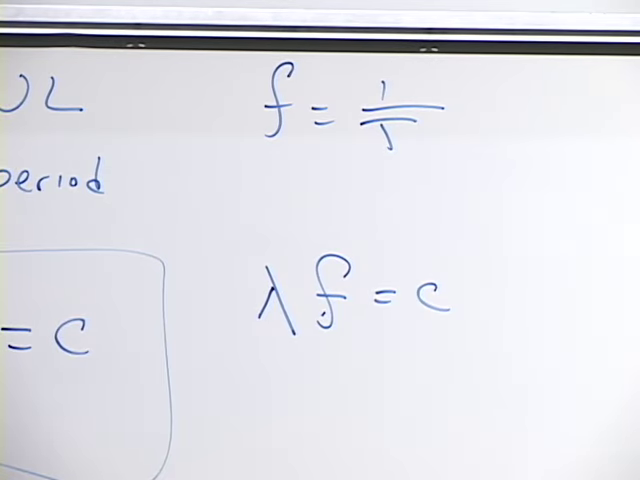
\includegraphics[width=0.68\textwidth]{lecture_01_figure_03.png}\caption{Für eine Lichtwelle gilt \(f=1/T\) und \(\lambda f=c\).}\lectureframe{00:36:24}\end{figure}

Physiker geben die Schwingungsrate oft in Radiant pro Sekunde statt in vollständigen Zyklen pro Sekunde an. Man stelle sich eine gleichförmige Bewegung auf einem Kreis vor. Führt der Punkt jede Sekunde \(f\) Umläufe aus und enthält jeder Umlauf \(2\pi\) Radiant, so ist seine Kreisfrequenz
\begin{equation}
\omega=2\pi f,
\qquad
\frac{\omega}{2\pi}=f.
\end{equation}
Vorerst ist dies eine Definition; auf die praktische Frage, ob dadurch die Anzahl der Faktoren \(2\pi\) sinkt, kommen wir später zurück.

Aus \(f=c/\lambda\) und \(\omega=2\pi f\) folgt
\begin{equation}
\omega=\frac{2\pi c}{\lambda},
\qquad
\omega\lambda=2\pi c.
\end{equation}
Bei einer anderen Wellenart tritt an die Stelle von \(c\) deren Ausbreitungsgeschwindigkeit.

\begin{figure}[h]\centering
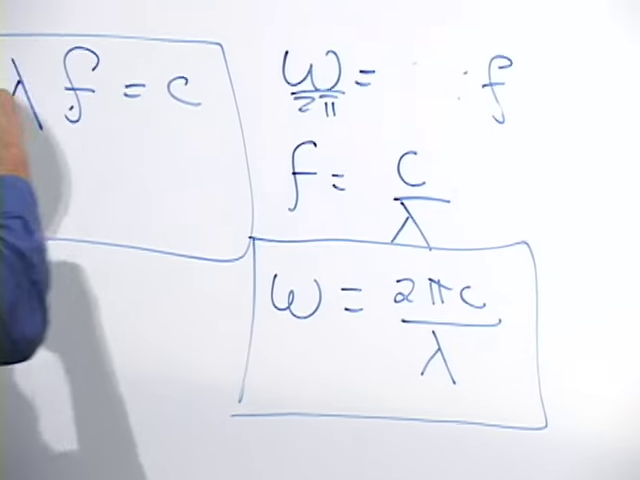
\includegraphics[width=0.68\textwidth]{lecture_01_figure_04.png}\caption{Für \(\omega=2\pi f\) gilt bei einer Lichtwelle \(\omega=2\pi c/\lambda\).}\lectureframe{00:39:10}\end{figure}

Elektromagnetische Strahlung bildet ein kontinuierliches Spektrum. In der üblichen Reihenfolge von längerer zu kürzerer Wellenlänge lauten die Bezeichnungen:
\begin{equation}
\begin{aligned}
\text{radio}
&\longrightarrow \text{microwave}
\longrightarrow \text{infrared}
\longrightarrow \text{visible}\\
&\longrightarrow \text{ultraviolet}
\longrightarrow \text{X ray}
\longrightarrow \text{gamma ray}.
\end{aligned}
\end{equation}
Sichtbares Licht nimmt nur einen schmalen Bereich ein. Die Grenzen zwischen den benannten Bereichen sind Konvention; hier benötigen wir daher keine exakten Grenzwellenlängen. Radiowellen können extrem lang sein; Gammastrahlung liegt am Ende des elektromagnetischen Spektrums mit den kürzesten Wellenlängen. Damit ist das Problem klar umrissen: Gammastrahlung ist klassisch eine kontinuierliche Feldwelle, wird aber in einzelnen Blips nachgewiesen.

\section{Diskrete Ankünfte und Wellenwahrscheinlichkeiten}

Thermodynamische Eigenschaften der Strahlung führten Planck und Einstein zu dem Schluss, dass Licht als diskrete Einheiten behandelt werden muss. Ein gedankliches Experiment veranschaulicht den Punkt, behauptet aber nicht, dass die Entdeckung tatsächlich auf diesem historischen Weg zustande kam.

Richtet man einen Strahl auf einen Schirm, erzeugt er bei gewöhnlicher Intensität einen zusammenhängend beleuchtet wirkenden Fleck. Setzt man einen teilweise lichtundurchlässigen Abschwächer in den Strahlengang, wird der Fleck dunkler. Erhöht man die Abschwächung wiederholt, trifft pro Zeiteinheit weniger Licht ein. Schließlich ändert sich das Erscheinungsbild. Statt eines kontinuierlich dunkler werdenden Flecks registriert der Detektor einzelne, isolierte Ereignisse.\footnote{Die schematische Darstellung rekonstruiert das Abschwächungsexperiment, das im Vorlesungsvideo zwischen 00:42:32 und 00:45:42 entwickelt wurde.}

\begin{figure}[h]\centering
\begin{tikzpicture}[scale=0.9]
\begin{scope}
\draw[fill=yellow!35] (0,0) circle (0.18);
\draw[->,thick] (0.2,0) -- (2.55,0);
\draw[thick] (2.65,-1.0) -- (2.65,1.0);
\node[below] at (1.4,-1.0) {\small bright beam};
\end{scope}
\begin{scope}[xshift=4.1cm]
\draw[fill=yellow!35] (0,0) circle (0.18);
\draw[->,thick] (0.2,0) -- (1.15,0);
\draw[fill=gray!70] (1.2,-0.85) rectangle (1.55,0.85);
\draw[->,thick] (1.6,0) -- (2.55,0);
\draw[thick] (2.65,-1.0) -- (2.65,1.0);
\node[below] at (1.85,-1.0) {\small strong attenuation};
\end{scope}
\fill[gray!45] (2.62,-0.65) rectangle (2.70,0.65);
\foreach \y in {-0.66,-0.31,0.13,0.58}
  \fill (6.72,\y) circle (0.045);
\node[above] at (2.65,1.0) {\small unresolved exposure};
\node[above] at (6.75,1.0) {\small isolated detections};
\end{tikzpicture}\caption{Durch schrittweise Abschwächung sinkt die Nachweisrate, bis sich aus einer kontinuierlich wirkenden Belichtung einzelne Photonenereignisse auflösen lassen.}\end{figure}

Wartet man lange genug, summieren sich die Ereignisse zum selben räumlichen Profil wie der ursprüngliche Fleck. Der helle Bereich war also die nicht aufgelöste Summe vieler einzelner Ankünfte. Dieses Experiment mit geringer Intensität lässt sich durchführen, war aber nicht das frühe Experiment, das ursprünglich die Photonhypothese nahelegte. Einsteins Photonenvorschlag entstand aus thermodynamischen und photoelektrischen Überlegungen; das Abschwächungsexperiment veranschaulicht seine Konsequenz besonders direkt.

Setzt man nun zwei Spalte in den Strahlengang und verringert die Intensität, bis die Photonen einzeln eintreffen, ist jede Detektion ein lokalisierter Blip. Nach vielen Detektionen füllen die Blips jedoch ein Interferenzmuster mit hellen und dunklen Streifen aus. Die einzelnen Ankünfte sind zufällig, doch ihre Wahrscheinlichkeitsverteilung entspricht der vom Wellenmuster vorhergesagten Verteilung. Die klassische Welle ist zu einer Welle geworden, die Wahrscheinlichkeiten bestimmt.

Welle und Teilchen sind also nicht zwei getrennte Arten von Entitäten, die verschiedenen Bereichen der Natur zugeordnet werden. Sie sind zwei Erscheinungsformen desselben Quantenobjekts. Licht lässt sich weder allein als Welle noch allein als Teilchen angemessen beschreiben.

Bei Elektronen kehrt sich die ursprüngliche Überraschung um. Elektronen gelten als Teilchen und treffen einzeln auf einen Detektor, doch bei hinreichend eng benachbarten Spalten erzeugen auch sie ein Interferenzmuster. Alphateilchen, die etwa achttausendmal schwerer sind als Elektronen, folgen demselben Prinzip, auch wenn das Experiment schwieriger ist. Interferenz wurde sogar mit Buckyballs beobachtet: Molekülen aus sechzig Kohlenstoffatomen, die ungefähr wie ein verallgemeinerter Fußball angeordnet sind. Es wird erwartet, dass dasselbe Prinzip sogar für Bowlingkugeln gilt, auch wenn ein solches Experiment praktisch völlig undurchführbar ist. Die Diskussion lässt sich auf vorgeschlagene Experimente mit Viren oder lebenden Zellen als zunehmend ambitionierte Beispiele ausweiten. Um zu verstehen, wie Wellen- und Teilchenbeschreibungen zusammenpassen, braucht man Quantenmechanik; zunächst geht es darum, die für die Teilchenphysik benötigten Eigenschaften der Photonen herauszuarbeiten.

\section{Photonenenergie}

Photonen sind die diskreten, unteilbaren Bestandteile des Lichts. Licht transportiert Energie---Sonnenlicht erwärmt einen absorbierenden Gegenstand---, also muss jedes Photon Energie tragen. Eine monochromatische Welle hat eine bestimmte Wellenlänge und Kreisfrequenz, und jedes Photon in ihr besitzt
\begin{equation}
E_\gamma=\hbar\omega.
\end{equation}
Der Versuch, sich eine kontinuierliche Welle als kleine mechanische Ansammlung von Punkten vorzustellen, führt in die Irre. Fest steht die experimentelle Kombination: Lokalisierte Detektionen treten mit einer wellenbestimmten Verteilung auf, und die Energie trifft in unteilbaren Einheiten ein.

Da
\begin{equation}
\omega=\frac{2\pi c}{\lambda},
\end{equation}
eine kürzere Wellenlänge eine größere Kreisfrequenz und damit mehr Energie pro Photon bedeutet,
\begin{equation}
\lambda\downarrow
\quad\Longrightarrow\quad
\omega\uparrow
\quad\Longrightarrow\quad
E_\gamma\uparrow.
\end{equation}
hat ein einzelnes Radiophoton sehr wenig Energie. Ein Radiostrahl kann dennoch insgesamt sehr viel Energie transportieren, wenn er sehr viele Photonen enthält. Für einen monochromatischen Impuls mit \(n\) Photonen gilt
\begin{equation}
E_{\text{pulse}}=n\hbar\omega,
\qquad
n=0,1,2,\ldots.
\end{equation}
Die Gesamtenergie kann groß sein, bleibt aber ein ganzzahliges Vielfaches der Energie eines einzelnen Photons.

Diese Beziehung führt zu der praktischen Frage, die den weiteren Verlauf der Diskussion bestimmen wird. Warum muss man immer größere Maschinen bauen, um immer kleinere Dinge zu sehen? Warum nicht eine kleine Maschine für ein kleines Objekt verwenden? Die erste Hälfte der Antwort liegt bereits vor: Um kleinere Strukturen aufzulösen, braucht man eine kürzere Wellenlänge, und ein Quant kürzerer Wellenlänge trägt mehr Energie.

\section{Ruheenergie und invariante Masse}

Die Teilchenphysik verbindet Quantenmechanik mit Relativitätstheorie. Die Photonenbeziehung \(E_\gamma=\hbar\omega\) liefert den quantenmechanischen Teil; die entsprechende elementare Tatsache aus der Relativitätstheorie lautet
\begin{equation}
E_{\mathrm{rest}}=mc^2.
\end{equation}
Die Einschränkung ist wichtig. Ältere Darstellungen unterschieden zwischen der \emph{Ruhemasse} und der geschwindigkeitsabhängigen \emph{bewegten Masse}. In der modernen Terminologie bezeichnet \emph{Masse} die invariante Masse eines Objekts. Bewegung verändert seine Energie, nicht seine Masse. Jedes Elektron hat dieselbe Masse, unabhängig von seinem Bewegungszustand, während die Energie eines Elektrons bei seiner Beschleunigung zunimmt. In dieser Form ist \(E=mc^2\) also die Energie eines massiven Objekts in einem Bezugssystem, in dem das Objekt als Ganzes ruht.

Das Objekt muss nicht im Inneren bewegungslos sein. Ein Gaskasten kann auf einer Waage stillstehen, während seine Moleküle sich rasch in alle Richtungen bewegen. Die Energie dieser inneren Bewegungen gehört zur Ruheenergie des gesamten Kastens. Man beginnt mit einem kalten Kasten, misst seine Masse und fügt dann Wärmeenergie hinzu, während der Kasten selbst in Ruhe bleibt. Seine Ruhemasse ändert sich um
\begin{equation}
\Delta m=\frac{\Delta E_{\mathrm{internal}}}{c^2}.
\end{equation}
Sein Gewicht und seine Trägheit nehmen mit seiner Masse zu. Bei einem gewöhnlichen Kasten ist der Effekt selbst nach einer großen Temperaturerhöhung auf einer gewöhnlichen Waage viel zu klein, um ihn zu bemerken; die geringe Größe des Effekts ändert nichts am Prinzip.

Ein prägnanteres Beispiel sind ein Elektron und ein Positron. Sie haben exakt gleiche Massen und entgegengesetzte elektrische Ladungen. Sind sie zunächst in Ruhe und vernichten sie sich gegenseitig, tragen Photonen die Energie davon:
\begin{equation}
e^-+e^+\longrightarrow \text{photons}.
\end{equation}
Die anfängliche Energie beträgt
\begin{equation}
E_{\mathrm{initial}}=2m_e c^2,
\end{equation}
und diese Energie kann nicht verschwinden. Ein einzelnes Paar liefert nur eine winzige Energiemenge. Um auch nur eine Tasse Kaffee zu erwärmen, wären daher enorm viele Paare nötig; einzelne Vernichtungsereignisse zeigen die Umwandlung jedoch unmittelbar.

Für ein ruhendes Objekt sind Masse und Energie somit dieselbe physikalische Größe, ausgedrückt in unterschiedlichen Einheiten. Der Faktor \(c^2\) ist der Umrechnungsfaktor zwischen den gebräuchlichen Masse- und Energieeinheiten, ähnlich einem Zahlenfaktor zur Umrechnung von Metern in Zentimeter.

\begin{classroomqa}\lecturetimestamp{01:04:39}\audiencequestion{Erfordert die Umwandlung von Masse in freigesetzte Energie einen Mechanismus?}\lecturerresponse{Ja, dafür ist ein physikalischer Mechanismus erforderlich, doch Erhaltungssätze schränken das Ergebnis bereits ein. Selbst bevor der mikroskopische Vernichtungsmechanismus beschrieben wird, muss die anfängliche Energie von Elektron und Positron irgendwo wieder auftauchen. Die Energieerhaltung kann daher einen wichtigen Teil der Antwort bestimmen, ohne dass die Wechselwirkung im Einzelnen erklärt wird.--}\end{classroomqa}

\section{Dimensionen und die Wahl der Einheiten}

In SI-Einheiten ist die Lichtgeschwindigkeit eine sehr große Zahl und das Plancksche Wirkungsquantum eine sehr kleine. Dass Letzteres klein ist, legt bereits die Photonenbeziehung nahe: Die Kreisfrequenz sichtbaren Lichts ist enorm, während die Energie eines einzelnen Photons winzig ist. Daher muss \(E_\gamma=\hbar\omega\) in diesen Einheiten einen kleinen Zahlenwert von \(\hbar\) erfordern. In der Größenordnung gilt
\begin{equation}
c\sim 10^8\ \mathrm{m\,s^{-1}},
\qquad
\hbar\sim 10^{-34}\ \mathrm{J\,s}.
\end{equation}
\editorialnote{Beibehalten werden nur die in der Vorlesung angegebenen Größenordnungen, da die letzten Ziffern an der Tafel undeutlich sind.}
Einheiten sind unverzichtbar: Keine der beiden Konstanten ist einfach eine dimensionslose Dezimalzahl. Da die Energie die Dimensionen
\begin{equation}
[E]=M L^2 T^{-2},
\end{equation}
hat und \(E_\gamma=\hbar\omega\) mit \([\omega]=T^{-1}\) gilt, hat das Plancksche Wirkungsquantum die Dimensionen
\begin{equation}
[\hbar]=[E]T=M L^2 T^{-1}.
\end{equation}

Wenn man \(c\) groß und \(\hbar\) klein nennt, setzt man bereits eine Einheitenwahl voraus. Misst man die Geschwindigkeit in Fuß pro Stunde, erhält man für \(c\) einen anderen Zahlenwert als bei der Messung in Metern pro Sekunde. In Lichtjahren pro Jahr oder Lichtsekunden pro Sekunde beträgt die Lichtgeschwindigkeit einfach eins. Durch eine geeignete abgestimmte Wahl der Einheiten für Masse, Länge und Zeit lässt sich ebenso \(\hbar=1\) setzen.

Vertraute Einheitensysteme sind überlieferte Konventionen und keine privilegierten Merkmale der Natur. Eine Meile umfasst 5280 Fuß, ein Stone entspricht vierzehn Pfund, Pferde misst man in Hand, und Leistung kann in Pferdestärken angegeben werden. Das metrische System ist systematischer, doch auch seine Maßstäbe sind menschliche Festlegungen. Nichts in der fundamentalen Physik zeichnet Meter, Sekunde oder Kilogramm besonders aus.

Länge, Zeit und Masse liefern drei unabhängige grundlegende Einheiten:
\begin{equation}
L,\qquad T,\qquad M.
\end{equation}
Andere mechanische Einheiten lassen sich daraus bilden. Welche Wahl nützlich ist, hängt vom Problem ab. In der Astrophysik ist die Sonnenmasse praktisch; in der Kernphysik kann die Protonenmasse nützlich sein; Lichtjahre und Jahre machen relativistische astronomische Formeln kompakt. Mit drei unabhängigen Wahlmöglichkeiten lassen sich drei unabhängigen dimensionsbehafteten Konstanten zweckmäßige Zahlenwerte zuweisen. Astrophysik, Atomphysik und Teilchenphysik müssen nicht dieselben Einheiten wählen.

Für die Teilchenphysik sind zwei Konventionen besonders nützlich:
\begin{equation}
c=1,
\qquad
\hbar=1.
\end{equation}
Für die verbleibende Einheit gibt es keine vergleichbar ausgezeichnete Teilchenmasse. Man könnte die Protonenmasse, die Higgs-Boson-Masse oder die Myonenmasse gleich eins setzen, würde damit aber lediglich ein Mitglied einer großen Gruppe bevorzugen.

Warum also \(c\) und \(\hbar\) wählen? Eine erste Antwort könnte lauten, dass sie in vielen Gleichungen vorkommen. Das häufige Auftreten reicht nicht aus: Auch die Protonenmasse erscheint in vielen Gleichungen, ebenso die Größe des Protons. Was \(c\) und \(\hbar\) auszeichnet, ist ihre Universalität.

Die Konstanten \(c\) und \(\hbar\) sind verschieden. Die Geschwindigkeit \(c\) setzt jedem physikalischen Objekt eine Grenze: Massive Objekte können sich ihr annähern, aber nicht über sie hinaus beschleunigt werden. Das Plancksche Wirkungsquantum begrenzt jedes Quantenobjekt durch die Unschärferelation in der Größenordnung
\begin{equation}
\Delta x\,\Delta p\gtrsim\hbar.
\end{equation}
Keine der beiden Aussagen zeichnet eine bestimmte Teilchenart aus. Diese Universalität macht \(c=1\) und \(\hbar=1\) zu natürlichen Konventionen.

Das Proton liefert keine vergleichbare universelle Skala. Es ist nur ein Objekt unter vielen. Die Protonenmasse gleich eins zu setzen, hätte keinen fundamentaleren Status, als die Masse eines Rubidiumatoms gleich eins zu setzen; Elektron, Higgs-Boson und Myon werfen dasselbe Problem auf.

Die elektrische Ladung legt eine weitere universelle Größe nahe; nachdem \(c\) und \(\hbar\) jedoch normiert wurden, ist die physikalisch bedeutsame elektromagnetische Kopplung dimensionslos. Durch eine Änderung der Einheiten lassen sich dimensionsbehaftete Konstanten in einer elektromagnetischen Formel verschieben; eine echte dimensionslose Kopplung lässt sich dadurch nicht ändern.

Die Gravitation liefert eine dimensionsbehaftete universelle Konstante. In der Newtonschen Form lautet der Betrag der Kraft zwischen zwei Massen
\begin{equation}
F=G\frac{m_1m_2}{r^2}.
\end{equation}
Jede Masse gravitativ wechselwirkt, wohingegen elektrisch neutrale Objekte nicht an einer elektrischen Kraft beteiligt sein müssen. Damit besitzt \(G\) die erforderliche Universalität. Für die gewöhnliche Teilchenphysik ist sie dennoch eine unpraktische Normierung, da die Gravitationskräfte zwischen bekannten Elementarteilchen in den hier betrachteten Rechnungen vernachlässigbar sind.

\begin{classroomqa}
\lecturetimestamp{01:20:34}
\audiencequestion{Ist es gerechtfertigt, \(G\) einfach außer Acht zu lassen? Bei sehr hohen Energien verhalten sich Elementarteilchen möglicherweise nicht gemäß der klassischen Gravitation, wie hier angenommen.}
\lecturerresponse{Einzelne Teilchen reagieren auf das Gravitationsfeld der Erde: Ein einzelnes Teilchen fällt in diesem Feld. Der Gravitationseinfluss eines Elementarteilchens auf ein anderes wurde nicht direkt gemessen; daher kann die Annahme der Universalität auf dieser Ebene infrage gestellt werden. Der unmittelbare Grund, \(G\) nicht zu berücksichtigen, ist praktischer, nicht grundsätzlicher Art: In gewöhnlichen teilchenphysikalischen Experimenten und Gleichungen ist der Beitrag der Gravitation vernachlässigbar klein.}
\end{classroomqa}

\begin{classroomqa}
\lecturetimestamp{01:22:01}
\audiencequestion{Könnte man statt der Gravitation die elektrische Wechselwirkung als dritte Konvention zur Festlegung der Einheiten verwenden?}
\lecturerresponse{Ja. Man kann elektromagnetische Einheiten wählen, in denen die elektrische Ladung oder die in Coulombs Gesetz auftretende Konstante normiert ist. Solche Konventionen werden verwendet. Elektronen stoßen einander ab, statt sich anzuziehen, doch dieses Vorzeichen steht einer solchen Wahl nicht entgegen. Hier wird diese Konvention lediglich nicht verwendet.}
\end{classroomqa}

\begin{classroomqa}
\lecturetimestamp{01:23:06}
\audiencequestion{Ist die elektrische Ladung dimensionslos, wenn \(c\) und \(\hbar\) gleich eins gesetzt werden?}
\lecturerresponse{Ja. Eine dimensionslose Größe, die mit dem Quadrat der elektrischen Ladung zusammenhängt, beträgt ungefähr \(1/137\). Die genaue Konvention und die Bedeutung dieser Zahl können zunächst zurückgestellt werden; hier kommt es darauf an, dass sie dimensionslos ist.}
\end{classroomqa}

\begin{classroomqa}
\lecturetimestamp{01:23:37}
\audiencequestion{Könnte man die Coulomb-Konstante als dritte Konstante wählen, die gleich eins gesetzt wird?}
\lecturerresponse{Sie lässt sich in die Konvention für elektromagnetische Einheiten aufnehmen. Damit kann die dimensionslose Kopplung \(1/137\) nicht auf eins gebracht werden, denn eine Änderung der Einheiten kann eine dimensionslose Zahl nicht verändern. Es wird kein besonderer Vorteil dafür beansprucht, hier diese Konvention zu verwenden.}
\end{classroomqa}

\section{Gleichungen in natürlichen Einheiten und Bezugssysteme}

Mit \(c=1\) nimmt die Ruheenergiebeziehung für ein massives Objekt die Form an
\begin{equation}
E_{\mathrm{rest}}=m.
\end{equation}
Mit \(\hbar=1\) nimmt die Beziehung für das Photon die Form an
\begin{equation}
E_\gamma=\omega.
\end{equation}
Die Konstanten können jederzeit wieder eingesetzt werden, wenn numerische Größen in konventionellen Einheiten benötigt werden.

\begin{figure}[h]
\centering
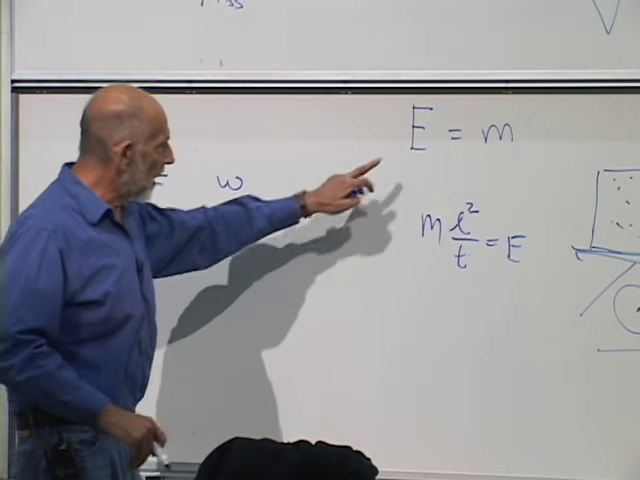
\includegraphics[width=0.72\textwidth]{lecture_01_figure_05.png}
\caption{In Einheiten mit \(c=1\) beträgt die Ruheenergie eines ruhenden massiven Objekts \(E=m\).}
\lectureframe{01:25:40}
\end{figure}

Diese Formeln sehen ähnlich aus, bedeuten aber Verschiedenes. In \(E_{\mathrm{rest}}=m\) ist \(E\) die Ruheenergie eines massiven Objekts. Ein Photon hat keine Masse und kann nicht in einen Ruhezustand gebracht werden; seine Energie ist daher keine Ruheenergie. Die Beziehung \(E_\gamma=\omega\) gibt die Energie eines bewegten, masselosen Quants an.

\begin{classroomqa}
\lecturetimestamp{01:26:07}
\audiencequestion{Was bedeutet \emph{in Ruhe}, wenn Ruhe immer relativ zu etwas ist und das Labor selbst nicht absolut ruht?}
\lecturerresponse{Ruhe wird relativ zu einem gewählten Bezugssystem definiert. Ist eine Tasse relativ zum Labor unbewegt, so ist ihre Energie in diesem Laborsystem ihre Masse, wenn \(c=1\); ein Beitrag aus einer Gesamtbewegung kommt dann nicht hinzu. Ein anderer Beobachter, der sich an der Tasse vorbeibewegt, schreibt ihr zusätzlich kinetische Energie zu. Verschiedene Beobachter ordnen demselben Objekt oder Photon im Allgemeinen unterschiedliche Energien zu: Energie ist bezugssystemabhängig, und die Annahme einer absoluten Ruhe ist nicht erforderlich.}
\end{classroomqa}

Die Konvention für die Kreisfrequenz lässt sich nun erneut betrachten. Die Schreibweise \(E_\gamma=\hbar\omega\) ist kompakt, doch \(\omega=2\pi f\) wurde zuvor ein Faktor \(2\pi\) eingeführt.

\begin{classroomqa}
\lecturetimestamp{01:28:13}
\audiencequestion{Warum verwendet man die Kreisfrequenz \(\omega\), gemessen in Radiant pro Sekunde, statt der scheinbar einfacheren Anzahl vollständiger Schwingungen pro Sekunde?}
\lecturerresponse{Die Wahl ist zum Teil historisch bedingt; die mathematische Antwort ist pragmatisch und nicht unmittelbar ersichtlich. Die hier vorgeschlagene Antwort ist vorläufig: Man schreibt die betreffenden Gleichungen einmal mit \(f\) und einmal mit \(\omega\) auf und prüft dann, bei welcher Konvention weniger Faktoren \(2\pi\) auftreten. Die Faktoren \(2\pi\) lassen sich nicht überall zugleich zum Verschwinden bringen. Außerdem wurde ein möglicher Zusammenhang mit der Schreibweise mithilfe komplexer Exponentialfunktionen angedeutet, hier aber nicht weiter ausgeführt.}
\end{classroomqa}

\begin{classroomqa}
\lecturetimestamp{01:29:51}
\audiencequestion{Kann man zwei Teilchen so weit beschleunigen, dass ihre gegenseitige Gravitationswechselwirkung wichtig wird?}
\lecturerresponse{Prinzipiell ja. In der Praxis sind heutige Beschleuniger von diesem Bereich außerordentlich weit entfernt. Die Antwort hängt auch davon ab, was mit einem Teilchen gemeint ist: Ein makroskopischer, gravitierender Körper ist nicht der hier betrachtete Fall eines Elementarteilchens.}
\end{classroomqa}

\begin{classroomqa}
\lecturetimestamp{01:30:27}
\audiencequestion{Was kann als Quelle für Positronen dienen?}
\lecturerresponse{Bei hochenergetischen Kollisionen können Positronen entstehen. Auch einige Kernprozesse und Zerfälle erzeugen sie.}
\end{classroomqa}

\begin{classroomqa}
\lecturetimestamp{01:30:53}
\audiencequestion{Sind die Planck-Zeit und die Planck-Länge die hier verwendeten natürlichen Einheiten?}
\lecturerresponse{Nein. Planck-Einheiten ergeben sich, wenn \(G\), \(c\) und \(\hbar\) alle gleich eins gesetzt werden. Die so erhaltene Planck-Länge ist viel kleiner als die Längenskalen der gewöhnlichen Teilchenphysik und daher hier ein unpraktisches Maß. Solche Einheiten sind dann natürlich, wenn Gravitation, Quantenmechanik und Relativität zugleich eine Rolle spielen, etwa in der Physik Schwarzer Löcher, der Kosmologie oder der Quantengravitation. Ist die Gravitation vernachlässigbar, ist es nützlicher, nur \(c\) und \(\hbar\) gleich eins zu setzen.}
\end{classroomqa}

\section{Impuls, Licht und Auflösungsvermögen}

Der nächste Grundbegriff ist der Impuls. Ein ruhendes Objekt hat keinen Impuls, obwohl es die von null verschiedene Ruheenergie \(mc^2\) besitzt. Sobald es sich bewegt, hat es im Allgemeinen Impuls. Bei einer Kollision ist der Impuls ebenso erhalten wie die Energie: Der gesamte Vektorimpuls ist vor und nach dem Zusammenstoß zweier Objekte gleich. Alles, was einem Erhaltungssatz unterliegt, verdient besondere Aufmerksamkeit.

Der Impuls ist ein Vektor: Er zeigt in Bewegungsrichtung. Für ein nichtrelativistisches Objekt gilt
\begin{equation}
\mathbf p=m\mathbf v.
\end{equation}
Dies ist nicht die allgemeine relativistische Formel und lässt sich nicht unmittelbar auf Licht anwenden.

Dennoch trägt Licht sowohl Impuls als auch Energie. Gewöhnliches Licht übt nur einen so kleinen Schub aus, dass sein Impuls schwer zu bemerken ist; ein intensiver Laserpuls kann jedoch einen beträchtlichen Impuls übertragen. Der große Laser in Livermore kann zum Beispiel Materie durch den von seiner Strahlung getragenen Impuls nach innen treiben.

Betrachten wir einen Puls, dessen Strahlen so gut gebündelt sind, dass sie sich nahezu entlang einer Achse bewegen. Ein realer Strahl kann eine gewisse Winkeldivergenz aufweisen, sodass sich Teile davon in leicht unterschiedlichen Richtungen ausbreiten. Für einen ideal gebündelten Strahl zeigt der Impuls jedoch entlang des Strahls und hat den Betrag
\begin{equation}
p=\frac{E}{c},
\qquad\text{or equivalently}\qquad
E=cp.
\end{equation}
Diese Beziehung wird hier als relativistische Tatsache angenommen und nicht hergeleitet. Die folgende Dimensionsprüfung bestätigt lediglich, dass ihre Einheiten mit denen des gewöhnlichen Impulses übereinstimmen:
\begin{equation}
\left[\frac{E}{c}\right]
=
\frac{M L^2 T^{-2}}{L T^{-1}}
=
M L T^{-1}
=
[m v]
=
[p].
\end{equation}
Dieser Dimensionsvergleich schreibt dem Licht keine Ruhemasse zu. Ein Photon hat die Masse null; es trägt Impuls, weil es Energie trägt und sich mit \(c\) bewegt.

Die Richtung von \(\mathbf p\) ist die Ausbreitungsrichtung. Sein Betrag ist gewöhnlich schwer nachzuweisen, weil \(c\) im Nenner steht. Ein Strahl kann seine Energie leicht dadurch zeigen, dass er Materie erhitzt oder verdampft, während sein mechanischer Schub viel kleiner ist. Bei hinreichend großer Intensität kann dieser Schub jedoch erheblich werden.

Für ein Photon gilt
\begin{align}
p_\gamma
&=\frac{E_\gamma}{c}\\
&=\frac{\hbar\omega}{c}.
\end{align}
Um dies durch die Wellenlänge auszudrücken, betrachten wir die Wellenbeziehungen noch einmal sorgfältig. Da
\begin{equation}
f\lambda=c,
\qquad
\omega=2\pi f,
\end{equation}
lautet die korrekte Beziehung
\begin{equation}
\omega\lambda=2\pi c,
\qquad
\omega=\frac{2\pi c}{\lambda}.
\end{equation}
Der Faktor \(2\pi\) lässt sich leicht vertauschen, wenn man die Definitionen nicht ausschreibt. Setzt man erneut bei \(f\lambda=c\) und \(f=\omega/(2\pi)\) an, ist die Frage geklärt:
\begin{equation}
\frac{\omega}{2\pi}\lambda=c
\quad\Longrightarrow\quad
\omega\lambda=2\pi c.
\end{equation}
Einsetzen ergibt nun
\begin{align}
p_\gamma
&=\frac{\hbar}{c}\frac{2\pi c}{\lambda}\\
&=\frac{2\pi\hbar}{\lambda}\\
&=\frac{h}{\lambda}.
\end{align}

\begin{classroomqa}
\lecturetimestamp{01:42:38}
\audiencequestion{Ist \(2\pi\hbar\) gleich \(h\)?}
\lecturerresponse{Ja. Per Definition gilt \(h=2\pi\hbar\); somit ist \(p_\gamma=2\pi\hbar/\lambda\) dasselbe wie \(p_\gamma=h/\lambda\). Unabhängig davon, welche Frequenzkonvention gewählt wird, treten Faktoren \(2\pi\) irgendwo wieder auf.}
\end{classroomqa}

Je kürzer die Wellenlänge, desto größer der Impuls des Photons. Ein Radiophoton hat eine sehr lange Wellenlänge und einen winzigen Impuls. Ein Gammaphoton hat eine sehr kurze Wellenlänge und überträgt einen viel stärkeren Stoß. Ein einzelnes Photon bewirkt makroskopisch weiterhin nur einen kleinen Impuls, doch sein Impuls ist viel größer als der eines Radiophotons. Auch seine Energie ist größer, denn \(E_\gamma=cp_\gamma\).

Dieser Zusammenhang erklärt, warum kleinere Objekte größere Maschinen erfordern. Ein Foto, das mit Wellenlängen aufgenommen wird, die viel größer als ein menschlicher Kopf sind, könnte nur eine unscharfe Silhouette zeigen. Um Gesichtszüge zu unterscheiden, muss die Wellenlänge kürzer als der Kopf sein. Um ein einzelnes Haar aufzulösen, muss sie mit dessen Dicke vergleichbar oder kleiner sein. Um die Struktur eines Atoms aufzulösen, darf die Wellenlänge der Sonde nicht größer als das Atom sein:
\begin{equation}
\lambda_{\mathrm{probe}}\lesssim
\text{size of the structure to be resolved}.
\end{equation}
Für kleinere Strukturen braucht man also kürzere Wellenlängen, und kürzere Wellenlängen erfordern größeren Impuls und höhere Energie. Die Sonde muss kein Photon sein; auch hochenergetische Teilchen anderer Art folgen demselben quantenmechanischen Zusammenhang zwischen Wellenlänge und Impuls. Zu ihrer Erzeugung braucht man Beschleuniger, die jedem Teilchen mehr und mehr Energie übertragen. Das Paar \(p_\gamma=h/\lambda\) und \(E_\gamma=\hbar\omega\) trägt die Argumentation: Eine höhere Sondenenergie erhöht den Impuls und verkürzt die Wellenlänge.

Seit ungefähr einem Jahrhundert wiederholt sich in der Teilchenphysik dasselbe Muster: höhere Energie, größerer Impuls, kürzere Wellenlänge und feinere räumliche Auflösung.

\begin{classroomqa}
\lecturetimestamp{01:46:57}
\audiencequestion{Gibt es eine theoretische untere Grenze für die Wellenlänge?}
\lecturerresponse{Möglicherweise. In der Nähe der Planck-Länge wird etwas Neues erwartet, doch diese Antwort ist vorläufig. Falls die räumliche Auflösung dort an eine Grenze stößt, liegt diese Skala immer noch etwa siebzehn Größenordnungen unter den Abständen, die am LHC untersucht werden. Heutige Experimente sind also enorm weit davon entfernt.}
\end{classroomqa}

Dieselbe Argumentation legt einen groben Zusammenhang zwischen der Größe eines Beschleunigers und der Skala nahe, die er auflösen kann.

\begin{classroomqa}
\lecturetimestamp{01:48:02}
\audiencequestion{Hängen die Wellenlänge oder die Größe der aufgelösten Struktur ungefähr umgekehrt mit der Größe des Beschleunigers zusammen?}
\lecturerresponse{Ungefähr ja, sofern die maximalen elektrischen Felder zur Beschleunigung der Teilchen und die Magnetfelder zu ihrer Führung durch die verfügbaren Anlagen vorgegeben bleiben. Ein Beschleunigungsgradient ist ein Energiegewinn pro Längeneinheit. Für einen Linearbeschleuniger der Länge \(L\) und mit annähernd konstantem Gradient \(\mathcal G\) gilt
\[
E_{\mathrm{beam}}\sim \mathcal G L.
\]
Bei ultrarelativistischen Energien ist die auflösbare Wellenlänge umgekehrt proportional zur Energie. Eine Vergrößerung der Länge des Linearbeschleunigers verbessert daher die Auflösung ungefähr um den umgekehrten Faktor. Dies ist nur eine heuristische Skalierung, kein exaktes Gesetz. In Kreisbeschleunigern kann dieselbe Anlage wiederholt durchlaufen werden; beim Ablenken strahlen beschleunigte Ladungen jedoch Energie ab.}
\end{classroomqa}

\begin{classroomqa}
\lecturetimestamp{01:49:47}
\audiencequestion{Wie groß müsste ein Beschleuniger sein, um die Planck-Länge zu erreichen?}
\lecturerresponse{Nach dieser groben Skalierung müsste er etwa siebzehn Größenordnungen länger sein als der Beschleuniger am CERN. Das wäre nicht so groß wie das Universum, aber ungefähr galaktischen Ausmaßes.}
\end{classroomqa}

\begin{classroomqa}
\lecturetimestamp{01:50:09}
\audiencequestion{Wie verhalten sich die Energien der höchstenergetischen kosmischen Strahlung zu den Kollisionsenergien in Beschleunigern?}
\lecturerresponse{Einzelne kosmische Strahlungsteilchen können eine weitaus höhere Energie im Laborsystem haben. Für den Zahlenvergleich betrachten wir ein extremes kosmisches Strahlungsteilchen mit einer Laborenergie in der Größenordnung von \(10^{21}\,\mathrm{eV}=10^{12}\,\mathrm{GeV}\). Ein kosmisches Strahlungsteilchen trifft jedoch auf ein ruhendes Target im Labor, während in einem Beschleuniger zwei energiereiche Strahlen frontal aufeinanderprallen. Noch wichtiger ist, dass aussagekräftige Experimente eine hohe Teilchenflussrate benötigen: viele Teilchen und viele gut kontrollierte Kollisionen. Ein einzelnes kosmisches Strahlungsteilchen kann das relevante Target verfehlen oder ein Ereignis erzeugen, aus dem sich nur wenig erschließen lässt. Eine bewusst übertriebene Schätzung des Ölbedarfs setzte die Menge, die für den Betrieb eines brauchbaren galaktischen Beschleunigers nötig wäre, mit etwa hundert Billionen Barrel Öl pro Sekunde an. Sie soll zeigen, dass genügend Kollisionsstatistik mindestens ebenso große Schwierigkeiten bereiten würde wie die Länge des Beschleunigers.}
\end{classroomqa}

\editorialnote{Die Umrechnung des Ölbedarfs ist in der Quelle widersprüchlich. Zunächst wird der Wert genannt und dann mit etwa \(10^{14}\) Barrel pro Sekunde wiederholt; eine spätere erneute Angabe lautet \(10^{11}\) Barrel pro Sekunde. Beide Größenordnungen bleiben erhalten, statt den Widerspruch stillschweigend aufzulösen.}

Dies sind tatsächliche Abstände und nicht bloß formale Größen. Die praktische Frage lautet, wie man sie untersuchen kann, ohne einen galaktischen Beschleuniger zu bauen und seine fantastisch hohe Leistung bereitzustellen.

\begin{classroomqa}
\lecturetimestamp{01:52:55}
\audiencequestion{Wie ist die Energie am LHC mit einem kosmischen Strahlungsteilchen der Energie \(10^{12}\,\mathrm{GeV}\) zu vergleichen?}
\lecturerresponse{Für ein ultrarelativistisches Projektil mit Laborenergie \(E_{\mathrm{lab}}\), das auf ein ruhendes Target der Masse \(m_{\mathrm{target}}\) trifft, skaliert die Schwerpunktsenergie parametrisch wie folgt:
\[
E_{\mathrm{cm}}\simeq
\sqrt{2m_{\mathrm{target}}c^2E_{\mathrm{lab}}}.
\]
\editorialnote{Der angezeigte Ausdruck für ein ruhendes Target macht die in diesem Austausch genannte Quadratwurzel-Skalierung ausdrücklich sichtbar.}
Bei festgehaltener Targetmasse wächst die nutzbare Kollisionsenergie daher nur mit der Quadratwurzel der Projektilenergie. Ein kosmisches Strahlungsteilchen mit \(10^{12}\,\mathrm{GeV}\) entspricht somit größenordnungsmäßig kollidierenden Strahlen mit Energien von \(10^6\,\mathrm{GeV}\) pro Strahl, nicht \(10^{12}\,\mathrm{GeV}\) in jedem Strahl. Kosmische Strahlung kann die Energien irdischer Beschleuniger zwar übertreffen, doch wegen ihrer äußerst geringen Flussrate sind systematische, kontrollierte Experimente unpraktisch.}
\end{classroomqa}
\chapter{Wellen, quantisierte Moden und Erzeugungsoperatoren}

\section{Wellen, Felder und komplexe Exponentialfunktionen}

Die Quantenfeldtheorie ist das grundlegende Werkzeug der Teilchenphysik. Bevor wir auch nur eine elementare Einführung in Quantenfelder geben, lohnt es sich, die mathematischen Tatsachen zusammenzustellen, die Wellen mit Teilchen verbinden. Eine Welle ist bereits eine Feldkonfiguration: Ein Feld nimmt an verschiedenen Raumpunkten unterschiedliche Werte an, und bei einer Welle schwingen diese Werte und breiten sich aus. Die Quantenmechanik stellt die Verbindung zwischen solchen Wellen und Teilchen her.

Quantenmechanik und spezielle Relativitätstheorie werden hier als bekannt vorausgesetzt. Es geht zunächst darum, die für die Teilchenphysik benötigten Grundlagen zu wiederholen, nicht darum, einen Kurs in einem dieser Fächer zu ersetzen.

Eine Exponentialfunktion ist durch proportionales Wachstum gekennzeichnet. Wenn
\begin{equation}
f(x)=e^{\alpha x},
\end{equation}
dann gilt
\begin{equation}
\frac{df}{dx}=\alpha f.
\end{equation}
Über ein kleines Intervall hinweg ist der Zuwachs proportional zu der bereits vorhandenen Menge. Eine Population, die in einer Petrischale wächst, veranschaulicht das auf vertraute Weise: Je mehr Organismen vorhanden sind, desto mehr können sich fortpflanzen, sodass die Zuwachsrate proportional zur Population selbst ist. Eine Multiplikation von \(e^{\alpha x}\) mit einer konstanten Gesamtgröße ändert an dieser definierenden Eigenschaft nichts.

Sinus und Kosinus schwingen, statt zu wachsen. Es handelt sich um dieselbe Kurve, um ein Viertel einer Periode gegeneinander verschoben, und beim Ableiten gehen sie ineinander über:
\begin{align}
\frac{d}{dx}\sin(kx)&=k\cos(kx),\\
\frac{d}{dx}\cos(kx)&=-k\sin(kx).
\end{align}
Keine der beiden Funktionen ist für sich allein eine Exponentialfunktion, denn ihre Ableitung ist proportional zur jeweils anderen Funktion. Die komplexe Kombination besitzt dagegen die Eigenschaft einer Exponentialfunktion. Mit \(i^2=-1\) gilt:
\begin{align}
\frac{d}{dx}\bigl(\cos(kx)+i\sin(kx)\bigr)
&=-k\sin(kx)+ik\cos(kx)\\
&=ik\bigl(\cos(kx)+i\sin(kx)\bigr).
\end{align}
Daher
\begin{equation}
e^{ikx}=\cos(kx)+i\sin(kx).
\end{equation}
Diese Identität begegnet uns immer wieder, weil sich wellenartige Schwingungen durch Sinus und Kosinus beschreiben lassen. Ist \(x\) eine Ortskoordinate, schwingt die Funktion im Raum. Ist das Argument die Zeit, schwingt sie zeitlich.

\section{Frequenz, Wellenlänge und Photonenimpuls}

Die gewöhnliche Frequenz \(f\) gibt die Anzahl vollständiger Perioden pro Sekunde an. Eine Periode ist eine vollständige Schwingung. Die Kreisfrequenz beschreibt dieselbe Bewegung in Radiant pro Sekunde:
\begin{equation}
\omega=2\pi f.
\end{equation}
Beide Schreibweisen beschreiben dieselbe Frequenz. Man wechselt zwischen ihnen, um unnötige Faktoren von \(2\pi\) aus einer Rechnung herauszuhalten; ganz verschwinden diese Faktoren allerdings nie.

Die Wellenlänge \(\lambda\) ist die Strecke, die eine vollständige räumliche Periode einnimmt. Breitet sich eine Welle mit der Geschwindigkeit \(v\) aus, dann ergibt das Produkt aus der Strecke pro Periode und der Anzahl der Perioden pro Sekunde ihre Ausbreitungsgeschwindigkeit:
\begin{equation}
\lambda f=v.
\end{equation}
Für Licht im Vakuum gilt \(v=c\), also
\begin{equation}
\lambda f=c.
\end{equation}
Bei einer Schallwelle steht auf der rechten Seite die Schallgeschwindigkeit, bei einer Wasserwelle die entsprechende Ausbreitungsgeschwindigkeit der Wasserwelle. Das Auftreten von \(c\) ist daher eine Aussage über Licht und keine Definition, die für alle Wellen gilt.

In der Quantenmechanik wird die Planck-Konstante in zwei Schreibweisen eingeführt:
\begin{equation}
\hbar=\frac{h}{2\pi}.
\end{equation}
Beim Wechsel von \(h\) zu \(\hbar\) werden lediglich Faktoren von \(2\pi\) von einer Gleichung in eine andere verschoben.

Die Zahlenwerte dimensionsbehafteter Konstanten hängen von den verwendeten Einheiten ab. Meter, Sekunden und Kilogramm sind am menschlichen Maßstab orientierte Konventionen, die für gewöhnliche Längen und Zeiten praktisch sind. Traditionelle Maße in der Größenordnung einer Armlänge waren für Stoffe oder Seile nützlich; unabhängig davon, wie genau es historisch zur Festlegung des Meters kam, gibt es kein fundamentales Prinzip, das gerade diese menschliche Größenskala auszeichnet. In SI-Einheiten gilt:
\begin{equation}
\begin{aligned}
h &\simeq 6.6\times10^{-34}\ \mathrm{J\,s},
&\hbar &\simeq 1.1\times10^{-34}\ \mathrm{J\,s},\\
c &\simeq 3\times10^8\ \mathrm{m\,s^{-1}}.
\end{aligned}
\end{equation}
Diese Zahlen sollen vor allem ihre Größenordnung in den gebräuchlichen Einheiten veranschaulichen: Die Planck-Konstante ist außerordentlich klein, die Lichtgeschwindigkeit außerordentlich groß.

Ein Quant einer Mode besitzt die Energie
\begin{equation}
E_{\text{one quantum}}=\hbar\omega=hf.
\end{equation}
Das ist die Energie eines einzelnen Photons, nicht die Gesamtenergie einer beliebigen klassischen elektromagnetischen Welle. Sichtbares Licht hat eine Frequenz in der Größenordnung von \(10^{15}\) Perioden pro Sekunde, sodass ein typisches optisches Photon eine Energie in der Größenordnung von
\begin{equation}
E_\gamma\sim 10^{-19}\ \mathrm{J}.
\end{equation}
besitzt. Selbst eine so schnelle optische Schwingung entspricht pro Quant einer sehr kleinen Energie, weil \(h\) so klein ist. Eine makroskopische Menge optischer Energie enthält daher eine enorm große Anzahl von Photonen.

Energie und Impuls verdienen besondere Aufmerksamkeit, denn beide Größen sind erhalten. Sie dienen als nützliche Buchhaltungsgrößen: Die Gesamtenergie und der Gesamtimpuls, die in einen Prozess hineingehen, müssen mit der Gesamtenergie und dem Gesamtimpuls übereinstimmen, die ihn verlassen. Der Impuls ist ein Vektor und zeigt in Bewegungsrichtung. Für ein Teilchen, das sich viel langsamer als Licht bewegt, gilt
\begin{equation}
\vec p=m\vec v.
\end{equation}

Betrachten wir nun elektromagnetische Strahlung, die in eine Richtung gebündelt ist, statt sich in viele Richtungen auszubreiten. Ihr Impuls zeigt entlang des Strahls. Die nichtrelativistische Formel lässt sich nicht auf ein Photon anwenden, denn \(m\) bezeichnet die Ruhemasse, und ein Photon hat keine Ruhemasse. Es gibt jedoch eine nützliche Dimensionsstütze. Weist man dem Photon \(E/c^2\) einmal \emph{unpassenderweise} wie eine Masse zu und setzt dann \(v=c\) ein, erhält man
\begin{equation}
mv\longrightarrow \frac{E}{c^2}c=\frac{E}{c}.
\end{equation}
Dieses Vorgehen liefert zufällig das richtige Ergebnis und die richtigen Einheiten. Es ist aber kein zulässiges Argument dafür, dass ein Photon die Ruhemasse \(E/c^2\) besitzt. Die tatsächliche relativistische Aussage für gebündelte Strahlung lautet
\begin{equation}
|\vec p|=\frac{E}{c}.
\end{equation}
Die Gleichung gibt den Betrag an. Die Richtung ist die Ausbreitungsrichtung der Strahlung.

Für ein einzelnes Photon gilt
\begin{align}
|\vec p_\gamma|
&=\frac{E_\gamma}{c}
=\frac{hf}{c}.
\end{align}
Für Licht gilt
\begin{equation}
\lambda f=c,
\qquad
\frac{f}{c}=\frac{1}{\lambda},
\end{equation}
und daher
\begin{equation}
|\vec p_\gamma|=\frac{hf}{c}=\frac{h}{\lambda}.
\end{equation}

\begin{figure}[t]\centering
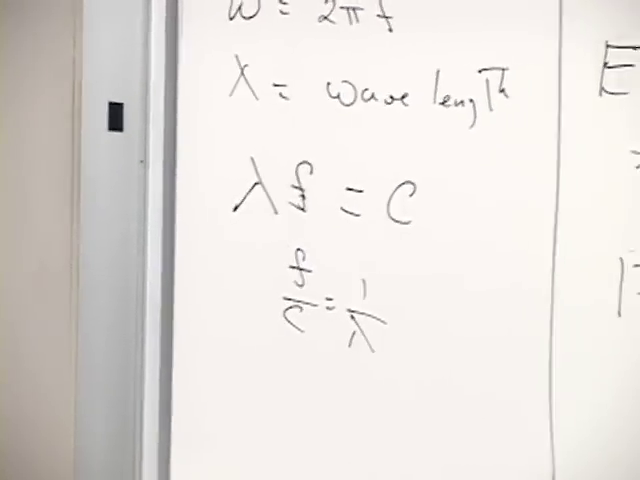
\includegraphics[width=0.56\textwidth]{lecture_02_figure_02.png}\caption{Für Licht gelten \(\lambda f=c\) und \(f/c=1/\lambda\), die Beziehungen, aus denen \(|\vec p_\gamma|=h/\lambda\) folgt.}\lectureframe{00:21:39}\end{figure}

Je kürzer die Wellenlänge, desto größer der Photonenimpuls. Das ist eine der wichtigsten quantenmechanischen Tatsachen für die Teilchenphysik. Um ein kleines Objekt zu untersuchen, braucht man eine Sonde mit kurzer Wellenlänge; der Preis dafür ist ein großer Impuls.

\begin{classroomqa}\lecturetimestamp{00:22:23}\audiencequestion{Ist \(E=\hbar\omega\) fundamental oder lässt es sich aus einem tiefer liegenden Prinzip herleiten?}\lecturerresponse{Es folgt aus der Quantenmechanik des harmonischen Oszillators. Dieses Ergebnis wird hier verwendet, ohne den Beweis zu wiederholen; die weiter unten entwickelte Beschreibung durch Oszillatoren liefert den tieferen Zusammenhang.}\end{classroomqa}


\section{Wellenamplitude und Photonenzahl}

\begin{classroomqa}\lecturetimestamp{00:23:10}\audiencequestion{Was bedeutet die Amplitude einer Welle in der Sprache der Photonen?}\lecturerresponse{Vergleichen wir zwei Wellen mit derselben Wellenlänge und Frequenz, aber unterschiedlicher Amplitude, zum Beispiel \(\sin(kx)\) und \(A\sin(kx)\). Klassisch ist die Energie in einem festen Raumbereich proportional zum Quadrat der Amplitude. Quantenmechanisch besitzt eine Mode mit \(n\) Photonen die Energie \(n\hbar\omega\). Bei fester Frequenz, festem Raumbereich und fester Normierung wächst die Amplitude daher größenordnungsmäßig wie \(\sqrt n\).}\end{classroomqa}

Die beiden Wellen haben dasselbe Schwingungsmuster. Eine ist lediglich stärker als die andere.\footnote{Die schematische Darstellung orientiert sich am Wellenvergleich bei 00:23:47--00:24:28.}

\begin{figure}[t]\centering
\begin{tikzpicture}[x=1cm,y=0.65cm]
\draw[->] (-0.4,0) -- (6.8,0);
\draw[->] (-0.4,-2.1) -- (6.8,-2.1);
\draw[thick] plot[domain=0:6.2,samples=120] (\x,{0.45*sin(\x r)});
\draw[thick] plot[domain=0:6.2,samples=120] (\x,{-2.1+1.15*sin(\x r)});
\draw (6.2,0.55) node[right]{small amplitude};
\draw (6.2,-0.75) node[right]{large amplitude};
\end{tikzpicture}\caption{Wellen mit gleicher Wellenlänge und Frequenz, aber unterschiedlichen Amplituden.}\end{figure}

Für eine feste Wellenmenge gilt:
\begin{equation}
E_{\text{wave}}\propto A^2.
\end{equation}
Bei einer elektromagnetischen Welle ist das die vertraute Aussage, dass die Feldenergie proportional zum Quadrat der Feldstärke ist. Enthält dieselbe Mode \(n\) Photonen, gilt
\begin{equation}
E_{\text{wave}}=n\hbar\omega.
\end{equation}
Folglich gilt bei festgehaltener Mode, Frequenz, Normierung und festem Raumbereich:
\begin{equation}
A^2\propto n\hbar\omega,
\qquad
A\propto\sqrt n\quad\text{at fixed }\omega.
\end{equation}
Eine exakte Normierung wird hier nicht behauptet. Es kommt darauf an, welche Wellenmenge berücksichtigt wird: Verdoppelt man die Länge einer ansonsten gleichförmigen Welle, ändert sich ihre Gesamtenergie, ohne dass sich die lokale Amplitude ändert. Die Proportionalität lässt sich daher für einen festen Raumbereich verstehen, etwa für eine Wellenlänge.

Dabei ist noch eine spezifisch quantenmechanische Einschränkung zu beachten. Amplitude und Phase können nicht beide exakt wie klassische Größen festgelegt werden. Die Frage ``Wie groß ist die Amplitude eines Photons?'' ist daher mehrdeutig, wenn sie auf ein vollkommen scharf bestimmtes klassisches Feld abzielt. Setzt man dennoch \(n=1\), erhält man eine sinnvolle Größenordnung.

\begin{classroomqa}\lecturetimestamp{00:28:25}\audiencequestion{Gibt die vertikale Auslenkung in einer Zeichnung einer elektromagnetischen Welle die Position des Photons im Raum an?}\lecturerresponse{Nein. Die Ausbreitungsachse ist räumlich, während die vertikale Koordinate den Wert des elektrischen oder magnetischen Feldes darstellt. Der Impuls zeigt entlang der Ausbreitungsachse, nicht in Richtung der eingezeichneten Feldamplitude.}\end{classroomqa}

Die Welle kann sich in jede beliebige Raumrichtung ausbreiten, doch die vertraute Sinuskurve verwendet nur ihre horizontale Achse als Ortskoordinate. Die andere eingezeichnete Richtung gibt die Feldstärke an.

\begin{classroomqa}\lecturetimestamp{00:29:37}\audiencequestion{Wird die angegebene Photonenzahl innerhalb einer Wellenlänge oder einer Periode der Welle gezählt?}\lecturerresponse{Man kann einen festen Raumbereich wählen, zum Beispiel eine Wellenlänge. Deshalb gilt nur eine Proportionalität: Die Gesamtenergie und die Photonenzahl hängen auch davon ab, wie viel von der Welle einbezogen wird. Zwei, drei oder vier Wellenlängen enthalten bei gleicher Amplitude entsprechend mehr Energie als eine Wellenlänge.}\end{classroomqa}

\begin{classroomqa}\lecturetimestamp{00:30:17}\audiencequestion{Ist die Amplitude eines einzelnen Photons bedeutungslos?}\lecturerresponse{Sie ist nur als Größenordnungsaussage sinnvoll, die man erhält, indem man \(n=1\) setzt. Bei einer elektromagnetischen Mode spielen Informationen über das elektrische und das magnetische Feld eine den konjugierten Orts- und Impulsinformationen analoge Rolle. Die quantenmechanische Unschärfe begrenzt daher, wie genau sich eine klassische Amplitude festlegen lässt. Die Größenordnungsbeziehung bleibt nützlich.}\end{classroomqa}

Diese Fragen führen bereits zur Quantenfeldtheorie, in der sich die Beziehung zwischen Feldvariablen und Teilchenzahl präzise formulieren lässt. Für den Moment reichen die Proportionalitäten aus.

\section{Allgemeine Quantenbeziehungen und langsame Materiewellen}

Manche der für Photonen eingeführten Formeln gelten viel allgemeiner, andere dagegen nicht. Bevor wir uns den Elektronen zuwenden, lohnt es sich, die Gültigkeitsbereiche zu ordnen.

\begin{figure}[t]\centering
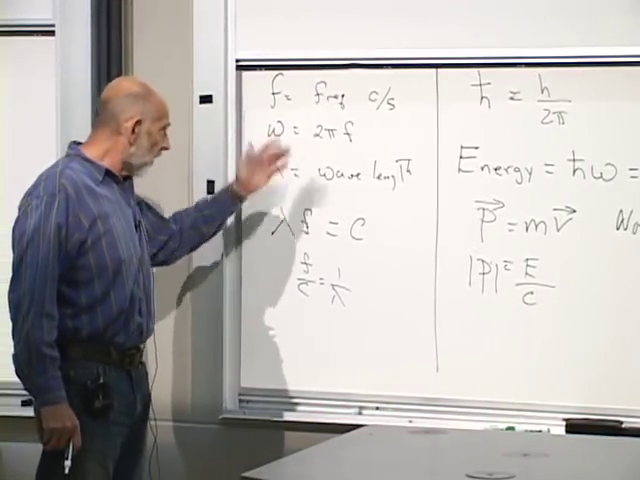
\includegraphics[width=0.82\textwidth]{lecture_02_figure_03.png}\caption{Wellendefinitionen sowie die Impulsbeziehungen für Photonen und nichtrelativistische Teilchen im Vergleich ihrer Gültigkeitsbereiche.}\lectureframe{00:31:52}\end{figure}

Die Definitionen von \(f\), \(\omega=2\pi f\) und \(\lambda\) gelten allgemein. Auch die Quantenbeziehung
\begin{equation}
E=\hbar\omega=hf
\end{equation}
ist in der vorliegenden Diskussion allgemein gültig. Formeln mit \(c\), etwa \(\lambda f=c\) und \(|\vec p|=E/c\), gelten dagegen für Wellen, die sich mit Lichtgeschwindigkeit ausbreiten. Die Formel \(\vec p=m\vec v\) gilt für Teilchen, die sich viel langsamer als Licht bewegen. Für relativistische Bewegungen zwischen diesen Grenzfällen wäre eine Interpolation erforderlich, die wir vorerst nicht benötigen.

Die Impuls--Wellenlängen-Beziehung gilt auch über das Photonbeispiel hinaus:
\begin{equation}
p=\frac{h}{\lambda}.
\end{equation}
Hier bezeichnet \(p\) den Betrag, wenn \(\lambda\) als positive Wellenlänge genommen wird; die Richtung lässt sich gesondert angeben.

\begin{figure}[t]\centering
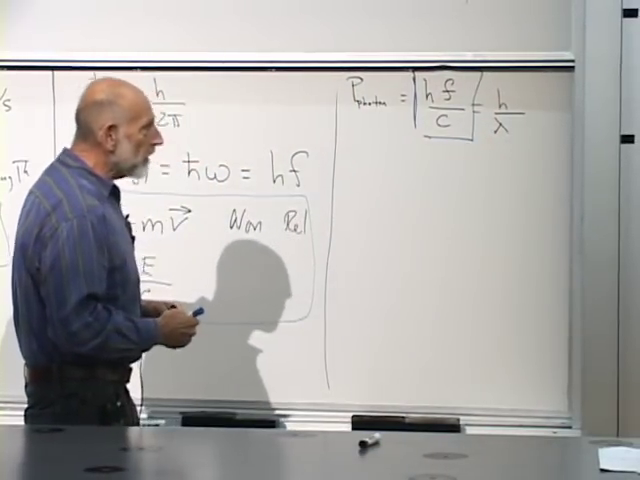
\includegraphics[width=0.74\textwidth]{lecture_02_figure_04.png}\caption{Photonenimpuls \(|\vec p_\gamma|=hf/c=h/\lambda\) als Ausgangspunkt für die allgemeine de-Broglie-Beziehung.}\lectureframe{00:33:32}\end{figure}

Mit einem Elektron, einem Atomkern und sogar einer Bowlingkugel lässt sich eine Welle verknüpfen. Die Interferenz von Elektronen ist eine Erscheinungsform dieser Tatsache. Schreiben wir die Elektronenwelle als \(\psi\). Was tritt bei einem langsam bewegten Elektron an die Stelle von \(\lambda f=c\)? Es fehlt noch die nichtrelativistische Beziehung zwischen Energie und Impuls.

Wir beginnen mit kinetischer Energie und Impuls:
\begin{align}
E&=\frac12 mv^2,\\
p&=mv,
\qquad
v=\frac{p}{m}.
\end{align}
Setzt man die letzte Beziehung in die erste ein, erhält man
\begin{align}
E
&=\frac12m\left(\frac{p}{m}\right)^2\\
&=\frac{p^2}{2m}.
\end{align}
In \(\frac12 mv^2\) steht die Masse im Zähler, in \(p^2/(2m)\) im Nenner. Diese Anordnung lässt sich leicht verwechseln und bei Bedarf einfach erneut herleiten.

Verwenden wir nun die allgemeinen Quantenbeziehungen
\begin{equation}
E=hf,
\qquad
p=\frac{h}{\lambda}.
\end{equation}
Für ein einzelnes langsames Teilchen gilt
\begin{align}
hf
&=\frac{p^2}{2m}\\
&=\frac{1}{2m}\left(\frac{h}{\lambda}\right)^2\\
&=\frac{h^2}{2m\lambda^2}.
\end{align}
Division durch \(h\) ergibt
\begin{equation}
f=\frac{h}{2m\lambda^2}.
\end{equation}

\begin{figure}[t]\centering
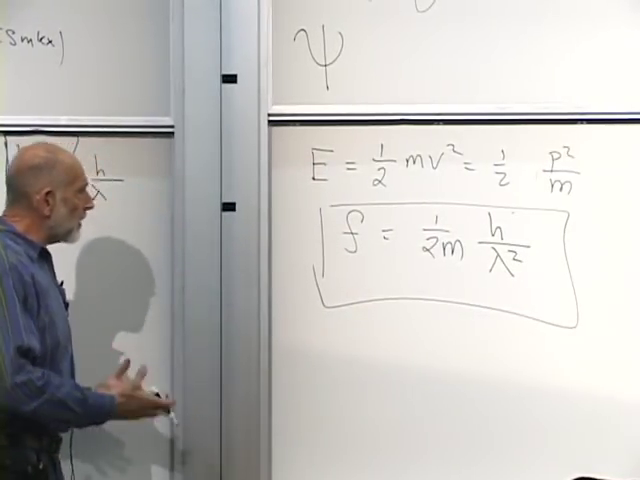
\includegraphics[width=0.64\textwidth]{lecture_02_figure_05.png}\caption{Für ein langsames Teilchen führen \(E=p^2/(2m)\) und \(p=h/\lambda\) auf \(f=h/(2m\lambda^2)\).}\lectureframe{00:37:47}\end{figure}

Für Licht gilt
\begin{equation}
f\propto\frac{1}{\lambda},
\end{equation}
während für langsame Materie gilt
\begin{equation}
f\propto\frac{1}{\lambda^2}.
\end{equation}
Die zweite Beziehung muss man nicht isoliert auswendig lernen. Sie lässt sich stets aus \(E=p^2/(2m)\), \(E=hf\) und \(p=h/\lambda\) rekonstruieren. Für ein langsam bewegtes Elektron in einem Atom gibt sie die Frequenz der zugehörigen Schr\"odinger-Welle an.

\begin{classroomqa}\lecturetimestamp{00:38:35}\audiencequestion{Gilt die nichtrelativistische Frequenz--Wellenlängen-Beziehung auch für andere Teilchen als Elektronen?}\lecturerresponse{Ja. Sie gilt für jedes Teilchen, das sich viel langsamer als Licht bewegt. Die relativistische Interpolation zwischen dem langsamen und dem lichtartigen Grenzfall ist ein eigenes Thema.}\end{classroomqa}

\begin{classroomqa}\lecturetimestamp{00:38:55}\audiencequestion{Welche Beziehung gilt für ein Neutrino?}\lecturerresponse{Das hängt von der Geschwindigkeit des Neutrinos ab. Die meisten Neutrinos, denen man in der Natur begegnet, bewegen sich sehr nahe an der Lichtgeschwindigkeit, sodass die lichtartige Beziehung eine gute Näherung ist. Ein Neutrino, das sich viel langsamer als Licht bewegt, würde dagegen der nichtrelativistischen Beziehung folgen.}\end{classroomqa}

\editorialnote{Ein kurzer Wortwechsel mit dem Publikum unmittelbar nach der Frage zum Neutrino dreht sich um Amplituden, Quanten und unterschiedliche Elektronenwellenlängen; sein Wortlaut ist jedoch zu stark beschädigt, um ihn zuverlässig wiederherzustellen. In der erhaltenen Antwort wird die allgemeine Beziehung zwischen Amplituden und Quanten unterschiedlicher Wellenlängen auf später verschoben.}

\begin{classroomqa}\lecturetimestamp{00:39:56}\audiencequestion{Ist ein Elektron aus einem \(20\,\mathrm{keV}\)-Beschleuniger langsam oder relativistisch?}\lecturerresponse{Es wird als langsam behandelt. In Einheiten mit \(c=1\) lassen sich Masse, Energie und Impuls in denselben Einheiten ausdrücken. Die Ruheenergieskala des Elektrons beträgt ungefähr \(0.5\,\mathrm{MeV}\), während \(20\,\mathrm{keV}\) viel kleiner ist. Gleichwertig dazu lautet das nichtrelativistische Impulskriterium \(p\ll mc\).}\end{classroomqa}

Der Energievergleich im Beispiel lautet
\begin{equation}
K=20\,\mathrm{keV}\ll m_ec^2\simeq0.5\,\mathrm{MeV}.
\end{equation}
\editorialnote{In der Passage bei 00:39:56--00:41:40 wird \(20\,\mathrm{keV}\) als Beschleunigerenergie eingeführt; das relativistische Kriterium wird anschließend als Vergleich des Impulses mit der Ruhemasse formuliert. Wenn man die Kriterien für kinetische Energie und Impuls getrennt angibt, setzt man die genannte Energie nicht mit einem Impuls gleich und bewahrt zugleich die Aussage, dass das Teilchen nichtrelativistisch ist.}

\section{Phasengeschwindigkeit, Gruppengeschwindigkeit und Dispersion}

\begin{classroomqa}\lecturetimestamp{00:41:46}\audiencequestion{Kann man die Geschwindigkeit einer Elektronenwelle bestimmen, indem man Frequenz und Wellenlänge multipliziert?}\lecturerresponse{Das ergibt die Phasengeschwindigkeit, nicht die dem Elektron zugeordnete Geschwindigkeit. Ein lokalisiertes Wellenpaket hat sowohl eine Phasengeschwindigkeit, die die Bewegung seiner inneren Wellenberge und -täler beschreibt, als auch eine Gruppengeschwindigkeit, die die Bewegung der Einhüllenden beschreibt. Die Gruppengeschwindigkeit wird mit der Bewegung des Teilchens identifiziert.}\end{classroomqa}

Ein Wellenpaket sieht lokal wie ein Sinus oder Kosinus aus, ist aber durch eine Einhüllende begrenzt. Bei seiner Ausbreitung müssen sich die Einhüllende und die Wellenberge in ihr nicht mit derselben Geschwindigkeit bewegen.\footnote{Die schematische Darstellung orientiert sich an der Erörterung von Wellenpaketen bei 00:42:34--00:44:11.}

\begin{figure}[t]\centering
\begin{tikzpicture}[x=0.75cm,y=0.8cm]
\draw[->] (-0.5,0) -- (12.8,0);
\draw[thick] plot[domain=0:12,samples=140] (\x,{1.10*exp(-0.20*(\x-6)^2)});
\draw[thick] plot[domain=0:12,samples=140] (\x,{-1.10*exp(-0.20*(\x-6)^2)});
\draw[thick] plot[domain=0:12,samples=240] (\x,{1.10*exp(-0.20*(\x-6)^2)*sin(6*\x r)});
\draw[->] (4.1,1.45) -- (7.5,1.45);
\draw (5.8,1.8) node{group motion};
\draw[->] (7.0,-1.55) -- (8.3,-1.55);
\draw (8.7,-1.55) node[right]{phase motion};
\end{tikzpicture}\caption{Ein lokalisiertes Wellenpaket, dessen Einhüllende und innere Phase sich im Allgemeinen mit unterschiedlichen Geschwindigkeiten bewegen.}\end{figure}

Die Phasengeschwindigkeit ist die Geschwindigkeit der Wellenberge, Wellentäler und anderer Phasen gleicher Phase einer monochromatischen Komponente. Für die nichtrelativistische Dispersionsrelation gilt
\begin{equation}
v_\phi=f\lambda=\frac{h}{2m\lambda}.
\end{equation}
Sie hängt von der Wellenlänge ab. Komponenten mit unterschiedlichen Wellenlängen haben daher unterschiedliche Phasengeschwindigkeiten, sodass sich die Wellenberge durch das Paket bewegen und das Paket dispersieren kann. Die Gruppengeschwindigkeit ist die Geschwindigkeit des Pakets als Ganzes; sie wird mit der des Teilchens identifiziert.

Es gibt einen einfachen Sonderfall. Bewegen sich alle Wellenlängenkomponenten mit derselben Geschwindigkeit, stimmen Phasen- und Gruppengeschwindigkeit überein. Licht im Vakuum besitzt diese Eigenschaft: Jede Wellenlänge breitet sich mit \(c\) aus. Für langsame Teilchen gilt diese Beziehung nicht; dort ändert sich \(f\lambda\) mit \(\lambda\).

Die Gleichung
\begin{equation}
f=\frac{h}{2m\lambda^2}
\end{equation}
ist die freie Schr\"odinger-Gleichung in leicht verkleideter Form. Die Frequenz legt die zeitliche Abhängigkeit einer ebenen Welle fest, die Wellenlänge ihre räumliche Abhängigkeit, und die Schr\"odinger-Gleichung verknüpft beides. Umgekehrt ergibt das Einsetzen einer Welle mit fester Frequenz und Wellenlänge in die freie Schr\"odinger-Gleichung wieder diese Dispersionsrelation.

\begin{classroomqa}\lecturetimestamp{00:47:02}\audiencequestion{Kann die Phasengeschwindigkeit größer als die Lichtgeschwindigkeit sein?}\lecturerresponse{Ja. Die Phasengeschwindigkeit überträgt keine Information. Information und das lokalisierte Wellenpaket breiten sich mit der Gruppengeschwindigkeit aus; eine überlichtschnelle Phasengeschwindigkeit ermöglicht daher keine überlichtschnelle Signalübertragung.}\end{classroomqa}

\section{Endlicher Raum und diskreter Impuls}

Letztlich interessieren uns Wellen im unendlichen Raum, doch ein endliches System ist der sicherere Ausgangspunkt. Ein Computer kann Unendlichkeit nicht unmittelbar speichern oder verarbeiten. Zunächst formuliert man die Gleichungen für ein endliches System und bildet erst danach den Grenzfall, in dem dessen Größe beliebig groß wird. Diese Vorgehensweise ist in der gesamten Quantenmechanik, Quantenfeldtheorie und Teilchenphysik nützlich.

Wenn man mit einer Raumdimension beginnt, geht nichts Wesentliches verloren. Die Welle könnte sich auf einer Geigensaite, einem geschüttelten Seil oder in einer abstrakten eindimensionalen Welt befinden. Das naheliegendste endliche System ist ein Abschnitt der Länge \(L\) mit reflektierenden Enden. Eine Welle läuft zu einem Ende, wird reflektiert und läuft zurück. Das ist eine vollkommen zulässige reflektierende Randbedingung, hat aber einen Nachteil: Der Impuls ist innerhalb des Wellensystems nicht erhalten. Eine nach rechts laufende Welle trägt nach rechts gerichteten Impuls; nach der Reflexion trägt sie nach links gerichteten Impuls. Die Randfläche hat den Impuls übertragen und die Differenz aufgenommen.

Die Impulsumkehr an einem reflektierenden Ende lässt sich schematisch darstellen.\footnote{Die schematische Darstellung veranschaulicht die Argumentation zur reflektierenden Randbedingung bei 00:49:24--00:51:08.}

\begin{figure}[t]\centering
\begin{tikzpicture}[x=1cm,y=1cm]
\draw[thick] (0,0) -- (7,0);
\draw[very thick] (0,-0.45) -- (0,0.45);
\draw[very thick] (7,-0.45) -- (7,0.45);
\draw[->,thick] (1.0,0.35) -- (5.8,0.35) node[midway,above]{\(p>0\)};
\draw[->,thick] (5.8,-0.35) -- (1.0,-0.35) node[midway,below]{\(p<0\)};
\draw (3.5,-0.85) node{\(L\)};
\end{tikzpicture}\caption{Die Reflexion an den Enden eines endlichen Abschnitts kehrt den Impuls einer laufenden Welle um.}\end{figure}

Es gibt eine andere Möglichkeit, das System endlich zu machen und dabei den Impuls zu erhalten. Dazu identifiziert man die beiden Endpunkte des Abschnitts. Man kann sich das Ergebnis als Kreis vorstellen, doch dafür ist kein buchstäblicher Kreis erforderlich, der in eine zweite Dimension eingebettet ist. Die mathematische Aussage lautet schlicht, dass die Koordinate periodisch ist: Nach einer zurückgelegten Gesamtstrecke von \(L\) kehrt man zum selben Punkt zurück.

\begin{figure}[t]\centering
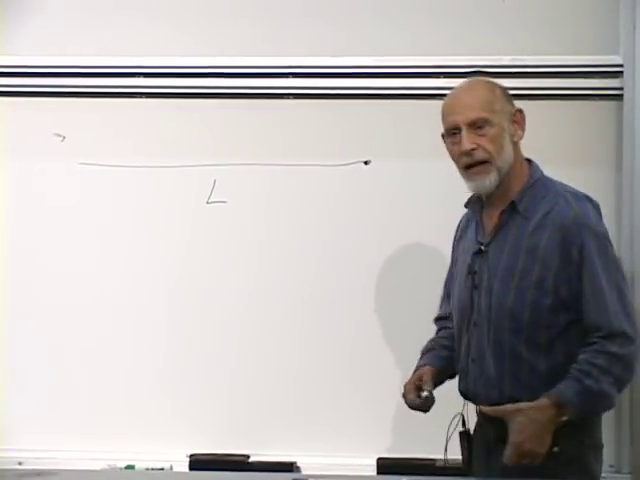
\includegraphics[width=0.72\textwidth]{lecture_02_figure_06.png}\caption{Ein eindimensionaler Weg der Gesamtlänge \(L\) zur Einführung der periodischen Identifikation.}\lectureframe{00:51:21}\end{figure}

Die Identifikation der Endpunkte ist in der folgenden schematischen Darstellung veranschaulicht.\footnote{Die schematische Darstellung orientiert sich an der Erörterung der periodischen Identifikation bei 00:51:09--00:52:37.}

\begin{figure}[t]\centering
\begin{tikzpicture}[x=1cm,y=1cm]
\draw[thick] (0,0) -- (7,0);
\fill (0,0) circle (1.5pt);
\fill (7,0) circle (1.5pt);
\draw[->,thick] (1.0,0.35) -- (6.0,0.35);
\draw (3.5,-0.35) node{\(L\)};
\draw[->,bend left=45] (7,0.08) to (0,0.08);
\draw (3.5,1.2) node{identified endpoints};
\end{tikzpicture}\caption{Eindimensionaler periodischer Raum, der durch Identifikation der Endpunkte eines Weges der Länge \(L\) entsteht.}\end{figure}

Eine nach rechts laufende Welle erreicht dann den dargestellten Endpunkt, tritt am Anfang wieder ein und läuft weiter nach rechts. Eine nach links laufende Welle setzt ihre Bewegung ebenfalls nach links fort. Es gibt keinen ausgezeichneten Endpunkt, an dem die Welle reflektiert würde, sodass sich der Impuls nicht umkehrt. Der periodische Raum macht das Volumen endlich und erhält den Impuls, hat aber eine wichtige Folge: Die möglichen Impulse sind diskret.

In die Gesamtlänge muss eine ganzzahlige Anzahl von Wellenlängen passen. Für eine nichtkonstante Mode gilt:
\begin{equation}
\lambda_{|N|}=\frac{L}{|N|},
\qquad |N|=1,2,3,\ldots .
\end{equation}
Die Wellenlänge kann also \(L\), \(L/2\), \(L/3\) und so weiter betragen. Eine Wahl wie \(L/\sqrt{2}\) passt nicht: Nach einem Umlauf würde die Welle mit der falschen Phase zurückkehren und nicht mit ihrem Anfangswert übereinstimmen.

Mit \(p=h/\lambda\) beträgt der Impulsbetrag der \(|N|\)-ten nichtkonstanten Mode
\begin{equation}
|p_N|=\frac{|N|h}{L}.
\end{equation}
Um beide Richtungen und die konstante Mode eindeutig zu berücksichtigen, ist es praktisch, die Modenbezeichnung vorzeichenbehaftet zu wählen:
\begin{equation}
p_N=\frac{Nh}{L},
\qquad N=0,\pm1,\pm2,\ldots .
\end{equation}
Positive und negative Werte von \(N\) stehen für entgegengesetzte Ausbreitungsrichtungen. Die Mode \(N=0\) ist konstant und hat den Impuls null; sie besitzt keine endliche Wellenlänge, die man in \(h/\lambda\) einsetzen könnte. Der grundlegende Impulsabstand beträgt daher \(h/L\).

Für ein makroskopisches \(L\) sind sowohl \(h\) als auch \(1/L\) groß, sodass dieser Impulsabstand äußerst klein ist. Die erlaubten Werte liegen dann sehr dicht beieinander und erscheinen nahezu kontinuierlich. Eine Perle, die auf einen kreisförmigen Draht beschränkt ist, besitzt trotzdem genau dieses diskrete Spektrum.

\begin{classroomqa}\lecturetimestamp{00:58:27}\audiencequestion{Wird der Gesamtimpuls der Welle quantisiert oder der Impuls einer einzelnen Periode?}\lecturerresponse{Die Aussage bezieht sich auf den Impuls jedes einzelnen Quants. Jedes Quant besitzt einen der erlaubten diskreten Impulse. Der Gesamtimpuls einer beliebigen Sammlung von Quanten ist daher ebenfalls ein ganzzahliges Vielfaches der Grundeinheit \(h/L\).}\end{classroomqa}

\begin{classroomqa}\lecturetimestamp{00:59:22}\audiencequestion{Warum muss die Welle nach einem Umlauf zu demselben Wert zurückkehren?}\lecturerresponse{Die identifizierten Endpunkte sind derselbe physikalische Punkt, daher muss ein beobachtbares Feld dort denselben Wert haben. Eine Abweichung würde an diesem Punkt einen plötzlichen Sprung des Feldes erfordern. Eine solche Unstetigkeit ist mit hohen Energie- und Impulskosten verbunden; zulässige Feldkonfigurationen sind stetig und periodisch.}\end{classroomqa}

\begin{classroomqa}\lecturetimestamp{01:00:09}\audiencequestion{Was passiert, wenn die Welle in einem Paket lokalisiert ist?}\lecturerresponse{Ein Paket ist eine Fourier-Summe ebener Wellen oder, gleichbedeutend, von Sinus- und Kosinusfunktionen. Im periodischen Raum darf diese Summe nur die diskreten, erlaubten Impulsmoden enthalten. Die Quantisierungsaussage bezieht sich somit auf die Fourier-Komponenten jedes zulässigen Pakets.}\end{classroomqa}

\begin{classroomqa}\lecturetimestamp{01:01:01}\audiencequestion{Gibt es ein Problem, wenn die periodische Länge \(L\) extrem klein wird?}\lecturerresponse{Wenn \(L\) abnimmt, wird der grundlegende Impuls \(h/L\) sehr groß. Bei gewöhnlichen mikroskopischen Längen folgt daraus kein unmittelbarer Widerspruch; für eine Fortsetzung der Konstruktion bis zur Planck-Längenskala dürfte jedoch neue Physik erforderlich sein.}\end{classroomqa}

Nehmen wir nun die Kreisvorstellung wörtlich: Eine Perle bewegt sich auf einem kreisförmigen Draht mit Radius \(r\) und Umfang \(L=2\pi r\). Ihre erlaubten tangentialen Impulse sind
\begin{equation}
p_N=\frac{Nh}{2\pi r}=\frac{N\hbar}{r}.
\end{equation}
Für ein nichtrelativistisches Teilchen auf einer Kreisbahn ist der Drehimpuls \(mvr\). Da in diesem Bereich \(p=mv\) gilt, ist er gleich \(rp\). Der Ausdruck \(mvr\) gilt nicht allgemein relativistisch, denn dann ist \(p\) nicht einfach \(mv\); das Produkt aus Impuls und senkrechtem Abstand bleibt jedoch die richtige Beziehung. In Vektorform lautet sie:\footnote{In der Vorlesung wird zunächst \(L\) für den Drehimpuls verwendet; dann fällt die Überschneidung mit \(L\) für die periodische Länge auf und es wird ein anderes Symbol gewählt. Hier wird durchgehend \(J\) verwendet; siehe 01:03:40--01:05:21.}
\begin{equation}
\vec J=\vec r\times\vec p,
\end{equation}
Bei einer tangentialen Kreisbewegung ist sein Betrag \(J=rp\). Somit gilt
\begin{equation}
J_N=rp_N=N\hbar.
\end{equation}
Der Abstand der linearen Impulse hängt von der Größe des Kreises ab, während die Einheit des Drehimpulses stets \(\hbar\) beträgt. Bei Fermionen gibt es Ausnahmen von der Ganzzahligkeitsregel; darauf gehen wir später ein.

Als Nächstes soll die Beziehung zwischen Feldern, Teilchen und Quanten präziser hergestellt werden. Dafür ist ein kurzer Rückgriff auf die Quantenmechanik von Operatoren und den harmonischen Oszillator nötig.

\section{Wellenmoden und Quantenoperatoren}

Die folgende Quantenmechanik ist notwendigerweise abstrakt und als Wiederholung gedacht. Der harmonische Oszillator ist das entscheidende System, denn eine Welle ist eine Schwingung. An einem festen Punkt ändert sich die Amplitude eines elektrischen Feldes, eines magnetischen Feldes oder einer anderen Welle periodisch mit der Zeit; von einer Frequenz einer Komponente zu sprechen heißt bereits, dass sie schwingt.

Eine allgemeine Welle muss nicht nur eine einzige Wellenlänge haben. Licht verschiedener Farben kann miteinander gemischt werden; umgekehrt kann ein Prisma gemischtes Licht in seine einzelnen Farben zerlegen, wie Newton es bei der Zerlegung weißen Lichts tat. Jede Komponente hat ihre eigene Wellenlänge, Frequenz, Amplitude, Energie und ihren eigenen Impuls. Die gemischte Welle lässt sich somit in Quanten unterschiedlicher Energien und Impulse zerlegen. Jede Wellenlänge legt eine Frequenz fest, und jede Komponente mit bestimmter Frequenz verhält sich wie ein Oszillator. Deshalb ist der harmonische Oszillator der natürliche Baustein eines Feldes und nicht ein beliebiges Quantensystem.

Quantenmechanische Observablen werden durch Operatoren dargestellt. Operatoren lassen sich addieren und multiplizieren, doch anders als bei gewöhnlichen Zahlen muss das Produkt nicht unabhängig von der Reihenfolge sein. Seien \(A\) und \(B\) Darstellungen zweier Eigenschaften eines Systems, die jeweils für sich messbar sein könnten. So könnte \(A\) beispielsweise ein elektrisches Feld und \(B\) ein magnetisches Feld darstellen. Sind die Messwerte die gewöhnlichen Zahlen \(a\) und \(b\), dann gilt
\begin{equation}
ab=ba.
\end{equation}
Ihr numerisches Produkt kann nicht von der Reihenfolge der Multiplikation abhängen. In der Quantenmechanik können die entsprechenden Operatoren dagegen stattdessen \(AB-BA\neq0\) erfüllen.

Auf den ersten Blick scheint das unsinnig. Wenn die Messung des elektrischen Feldes eine Zahl und die des magnetischen Feldes eine andere ergibt, muss das Produkt dieser beiden Zahlen in beiden Reihenfolgen dasselbe Ergebnis liefern. Die Auflösung besteht darin, dass sich zwei Größen nicht gleichzeitig messen lassen, wenn ihre Operatorprodukte von der Reihenfolge abhängen. Das Experiment zur Messung der einen Größe stört die Messung der anderen. Es liegt kein Widerspruch vor, denn die beiden Zahlenwerte lassen sich nicht gemeinsam bestimmen.

Wenn sich zwei Größen gleichzeitig messen lassen, sind ihre Messwerte gewöhnliche Zahlen und kommutieren miteinander. Ob sie gleichzeitig messbar sind, prüft man daher mit dem Kommutator
\begin{equation}
[A,B]=AB-BA.
\end{equation}
Ein verschwindender Kommutator bedeutet, dass die Observablen miteinander verträglich sind; ein von null verschiedener Kommutator bedeutet, dass sich die entsprechenden Messungen gegenseitig stören. Vertauscht man die Einträge, ändert sich das Vorzeichen:
\begin{equation}
[B,A]=-[A,B].
\end{equation}

Bei einem nichtrelativistischen Teilchen kommutieren die drei Ortskomponenten untereinander, und ebenso die drei Impulskomponenten:
\begin{align}
[x,y]&=[y,z]=[z,x]=0,\\
[p_x,p_y]&=[p_y,p_z]=[p_z,p_x]=0.
\end{align}
Alle drei Koordinaten lassen sich gemeinsam festlegen, ebenso alle drei Impulskomponenten. Entsprechende Orts- und Impulskomponenten kommutieren dagegen nicht:
\begin{equation}
[x,p_x]=[y,p_y]=[z,p_z]=i\hbar,
\end{equation}
Gemischte Komponenten wie \([x,p_y]\) verschwinden hingegen. Eine Messung einer Ortskoordinate versetzt den Teilchenimpuls in der dazu konjugierten Richtung in Unruhe. Anders ausgedrückt: Das Produkt der entsprechenden Unsicherheiten von Ort und Impuls wird durch \(\hbar\) bestimmt.

\begin{classroomqa}\lecturetimestamp{01:16:30}\audiencequestion{Ändert sich beim Wechsel von \(x\) zu \(y\) das \(i\) im Kommutator zu \(j\)?}\lecturerresponse{Nein. Das Symbol \(i\) bezeichnet immer die imaginäre Einheit, also die Quadratwurzel aus minus eins. Es ist weder die Bezeichnung eines kartesischen Einheitsvektors noch eines der Quaternionensymbole \(i,j,k\).}\end{classroomqa}

\begin{classroomqa}\lecturetimestamp{01:17:24}\audiencequestion{Bedeutet \(AB-BA\), zuerst \(A\) und dann \(B\) zu messen und anschließend die Messreihenfolge umzukehren?}\lecturerresponse{Nein. Die beiden Terme sind Operator- oder Matrixprodukte in unterschiedlicher algebraischer Reihenfolge. Sie bezeichnen keine wörtliche Abfolge von Messungen. Der Zusammenhang mit nicht miteinander verträglichen Messungen folgt aus der Operatoralgebra; er ist nicht die Definition des Produkts.}\end{classroomqa}

\begin{classroomqa}\lecturetimestamp{01:18:32}\audiencequestion{Gelten diese Kommutatoren von Ort--Impuls unmittelbar auch für ein Photon?}\lecturerresponse{Nicht unmittelbar. Sie gelten in klarer Form für nichtrelativistische Teilchen. Die Position eines Photons lässt sich schwieriger definieren; die analoge Aussage erfordert daher mehr Sorgfalt und wird hier nicht benötigt.}\end{classroomqa}

\section{Der quantenmechanische harmonische Oszillator}

Ein Gewicht an einer Feder, eine Schallwelle und eine Lichtwelle sind Beispiele für Schwingungen. Jeder ideale harmonische Oszillator hat eine Frequenz. Bei einer Feder ist eine volle Periode nicht einfach die Zeit, bis das Gewicht wieder dieselbe Position erreicht; es muss diese Position auch in derselben Richtung durchlaufen. Die Zahl der vollständigen Perioden pro Sekunde ist \(f\), und es gilt \(\omega=2\pi f\).

Klassisch kann ein idealer Oszillator jede nichtnegative Energie haben. Ein sanfter Stoß verleiht ihm wenig Energie, ein kräftigerer mehr. Eine reale Feder würde irgendwann brechen oder schmelzen, doch die mathematische Idealisierung besitzt ein kontinuierliches Spektrum positiver Energien. Beim Quantenoszillator ist das anders: Seine erlaubten Energien bilden eine diskrete, gleichmäßig abgestufte Leiter. Wählt man den Energienullpunkt so, dass das niedrigste Niveau null heißt, gilt
\begin{equation}
E_n=n\hbar\omega,
\qquad n=0,1,2,\ldots .
\end{equation}
Die gleichmäßig abgestuften Niveaus lassen sich wie folgt veranschaulichen.\footnote{Das Energieniveauschema folgt der Tafelbesprechung bei 01:21:20--01:23:56.}

\begin{figure}[t]\centering
\begin{tikzpicture}[x=1cm,y=0.9cm]
\draw[->] (0,0) -- (0,5.35);
\draw (0,5.5) node[above]{energy};
\foreach \y/\lab in {0.6/{0},1.6/{\hbar\omega},2.6/{2\hbar\omega},3.6/{3\hbar\omega},4.6/{n\hbar\omega}}
{
  \draw[thick] (0.2,\y) -- (2.2,\y);
  \draw (-0.25,\y) node[left]{\(\lab\)};
}
\draw[->,thick] (2.8,0.68) -- (2.8,1.52);
\draw (3.2,1.1) node[right]{\(a_+\)};
\draw[->,thick] (3.7,1.52) -- (3.7,0.68);
\draw (4.1,1.1) node[right]{\(a_-\)};
\end{tikzpicture}\caption{Gleichmäßig abgestufte Oszillatorniveaus gemäß der Konvention \(E_n=n\hbar\omega\).}\end{figure}

Der Abstand \(\hbar\omega\) ist dieselbe Energie, die zuvor einem Photon mit der Kreisfrequenz \(\omega\) zugeordnet wurde. Der Wert \(2\hbar\omega\) könnte die Energie eines einzelnen Quants eines Oszillators mit der Frequenz \(2\omega\) sein oder die Energie zweier Quanten in einem Oszillator mit der Frequenz \(\omega\). Hier wird die zweite Deutung benötigt. Ein einzelner Oszillator mit fester Frequenz kann null, ein, zwei, drei oder mehr Quanten enthalten; Energien zwischen den Stufen sind nicht erlaubt.

Die ganze Zahl \(n\) bezeichnet den Oszillatorzustand, geschrieben als Ket \(|n\rangle\). Der Zustand \(|0\rangle\) ist der Grundzustand, \(|1\rangle\) enthält ein Anregungsquant, \(|2\rangle\) zwei und so weiter. Das Ket ist lediglich die Schreibweise für den Zustand, auf den Operatoren wirken.

Wir definieren einen Erzeugungsoperator \(a_+\), der einen Zustand um eine Stufe anhebt, und einen Vernichtungsoperator \(a_-\), der ihn um eine Stufe absenkt:
\begin{align}
a_+|n\rangle &= \sqrt{n+1}\,|n+1\rangle,\\
a_-|n\rangle &= \sqrt{n}\,|n-1\rangle.
\end{align}
Die numerischen Quadratwurzelfaktoren gehören zu den Definitionen. Auf den niedrigsten Zustand wirkt der Operator wie folgt:
\begin{equation}
a_-|0\rangle=0,
\end{equation}
denn unterhalb des Grundzustands gibt es keinen Zustand.

Hier ist es wichtig, gewöhnliche Zahlen von Operatoren zu unterscheiden. Die Bezeichnung \(n\) und Koeffizienten wie \(\sqrt n\) sind gewöhnliche Zahlen; sie kommutieren mit allem. Die Symbole \(a_+\) und \(a_-\) stehen für Operatoren, deren Reihenfolge erhalten bleiben muss.

Wir senken zunächst \(|n\rangle\) um eine Stufe ab und heben es dann wieder an. Beim Absenken ergibt sich
\begin{equation}
a_-|n\rangle=\sqrt n\,|n-1\rangle.
\end{equation}
Die Wirkung von \(a_+\) auf den so erhaltenen Zustand liefert einen weiteren Faktor \(\sqrt n\), denn das Anheben von \(|n-1\rangle\) führt zurück zu \(|n\rangle\):
\begin{align}
a_+a_-|n\rangle
&=a_+\bigl(\sqrt n\,|n-1\rangle\bigr)\\
&=\sqrt n\,\sqrt n\,|n\rangle\\
&=n|n\rangle.
\end{align}
Somit liest \(a_+a_-\) die Stufennummer ab. Nehmen wir zum Beispiel an, \(|\chi\rangle\) sei bekanntermaßen ein Eigenzustand der Teilchenzahl, aber seine Stufenbezeichnung sei unbekannt. Gilt
\begin{equation}
a_+a_-|\chi\rangle=q|\chi\rangle,
\end{equation}
dann ist der gewöhnliche numerische Koeffizient \(q\) die Zahl der Quanten in diesem Zustand. Das Produkt ist also der Teilchenzahloperator,
\begin{equation}
\hat n=a_+a_-,
\end{equation}
und in der gewählten Energiekonvention lautet der Hamiltonoperator
\begin{equation}
H=\hbar\omega\,a_+a_-.
\end{equation}
Tatsächlich ergibt die Wirkung auf jede Stufe \(H|n\rangle=n\hbar\omega|n\rangle\).

Vertauschen wir nun die Reihenfolge. Zuerst das Anheben ergibt \(\sqrt{n+1}|n+1\rangle\). Das anschließende Absenken führt zurück zu \(|n\rangle\) und liefert einen zweiten Faktor \(\sqrt{n+1}\):
\begin{align}
a_-a_+|n\rangle
&=a_-\bigl(\sqrt{n+1}\,|n+1\rangle\bigr)\\
&=\sqrt{n+1}\,\sqrt{n+1}\,|n\rangle\\
&=(n+1)|n\rangle.
\end{align}
Die beiden Reihenfolgen unterscheiden sich bei jedem Zustand um eins, also gilt
\begin{equation}
[a_-,a_+]=a_-a_+-a_+a_-=1.
\end{equation}

Der Oszillator hat außerdem eine Amplitude und eine Phase. Seine Phase gibt an, an welcher Stelle seines Zyklus er sich befindet; konkret kann man sie durch den Zeitpunkt festlegen, an dem der Oszillator den Ursprung in einer gewählten Richtung durchläuft. Eine Verzögerung dieses Durchgangs ändert die Phase, nicht aber die Frequenz. Die Leiteroperatoren verbinden die quantenmechanischen Variablen, die zu Amplitude und Phase gehören. Ihre Algebra ist genuin quantenmechanisch, doch ihre Wirkung ist einfach: \(a_+\) fügt der Oszillatorenergie ein Quant hinzu und \(a_-\) entfernt eines. Bei einem elektromagnetischen Modus sind diese Quanten Photonen; deshalb nennt man die beiden Operatoren Erzeugungs- und Vernichtungsoperator.

\begin{classroomqa}\lecturetimestamp{01:37:34}\audiencequestion{Entsprechen die Erzeugungs- und Vernichtungsoperatoren einer physikalischen Messung?}\lecturerresponse{Die Photonenzahl ist messbar. Die Operatoren \(a_+\) und \(a_-\) sind aus weiteren technischen Gründen keine Observablen, die sich einzeln messen lassen. Ihr Kommutator zeigt, dass sie nicht miteinander kommutieren; dieser Umstand allein begründet jedoch nicht, dass einer der beiden für sich genommen unbeobachtbar ist.}\end{classroomqa}

Eine Anordnung von Federn mit unterschiedlichen Eigenfrequenzen ergibt viele unabhängige Oszillatoren. Dasselbe gilt für die elektromagnetischen Moden eines Hohlraums: Eine Wellenlänge kann angeregt werden, ohne dass die anderen gleich stark angeregt sein müssen. In der Quantenmechanik fügen Erzeugungs- und Vernichtungsoperatoren den Quanten einer festen Frequenz in jedem unabhängigen Oszillator hinzu oder entnehmen sie ihm. Diese Beschreibung ist zentral, weil Teilchen genau mit solchen Quanten identifiziert werden.

\section{Ein Feld als Ansammlung von Oszillatoren}

Kehren wir zum periodischen eindimensionalen Raum mit der Gesamtlänge \(L\) zurück. Seine nichtkonstanten Moden haben die Wellenlängenbeträge
\begin{equation}
\lambda_N=\frac{L}{N},
\qquad N=1,2,3,\ldots ,
\end{equation}
und die entsprechenden nichtnegativen Kreisfrequenzen \(\omega_N\). Zum Vergleich mit dem zuvor betrachteten Impulsspektrum ist es nützlich, den vorzeichenbehafteten ganzzahligen Index mit \(M\) neu zu bezeichnen:
\begin{equation}
p_M=\frac{Mh}{L},
\qquad M=0,\pm1,\pm2,\ldots .
\end{equation}
Das Vorzeichen von \(M\) gibt die Ausbreitungsrichtung an.
\editorialnote{Bei 01:42:08--01:42:24 wird der Index der Frequenzmoden korrigiert: Statt über einen vorzeichenbehafteten Bereich läuft er nun von null aufwärts. Das Symbol \(M\) dient hier nur dazu, die vorzeichenbehaftete Impulsnotation von der nichtnegativen Bezeichnung der Frequenzmoden \(N\) zu unterscheiden; es führt keine unabhängigen Besetzungszahlen für \(+M\) und \(-M\) ein. Die Liste der nichtkonstanten Oszillatoren beginnt bei \(N=1\).}

Jede erlaubte Frequenz verhält sich wie ein harmonischer Oszillator. Energie kann unabhängig einer Frequenz und anschließend einer anderen zugeführt werden. Das ausführlichere erste Beispiel eines Quantenfeldes folgt in der nächsten Vorlesung; die Zustandsnotation ist jedoch bereits klar. Ordnet man die nichtkonstanten Moden von der größten Wellenlänge an aufwärts, schreibt man
\begin{equation}
|n_1,n_2,n_3,\ldots\rangle,
\end{equation}
wobei \(n_N=0,1,2,\ldots\) die Zahl der Quanten im Oszillator mit der Frequenz \(\omega_N\) bezeichnet. Der erste Eintrag gibt an, wie viele Quanten die Mode mit der größten Wellenlänge besetzen, der zweite die Zahl der Quanten in der Mode mit der nächstgrößeren Wellenzahl und so weiter bis ins Unendliche.

Die Harmonischen einer Saite machen diese Konstruktion anschaulich. Die Folge von der Grundschwingung über die nächsten beiden Harmonischen ist schematisch dargestellt.\footnote{Das Schema folgt der Besprechung der Saitenharmonischen bei 01:45:20--01:47:46.}

\begin{figure}[t]\centering
\resizebox{\linewidth}{!}{%
\begin{tikzpicture}[x=0.98cm,y=1cm]
\draw[gray] (0,2.5) -- (6,2.5);
\draw[thick] plot[domain=0:6,samples=120] (\x,{2.5+0.48*sin(30*\x)});
\fill (0,2.5) circle (1.4pt);
\fill (6,2.5) circle (1.4pt);
\node[right] at (6.25,2.5) {fundamental: \(\omega_1\)};

\draw[gray] (0,1.25) -- (6,1.25);
\draw[thick] plot[domain=0:6,samples=120] (\x,{1.25+0.42*sin(60*\x)});
\fill (0,1.25) circle (1.4pt);
\fill (3,1.25) circle (1.4pt);
\fill (6,1.25) circle (1.4pt);
\node[right] at (6.25,1.25) {second harmonic: \(2\omega_1\)};

\draw[gray] (0,0) -- (6,0);
\draw[thick] plot[domain=0:6,samples=120] (\x,{0.42*sin(90*\x)});
\fill (0,0) circle (1.4pt);
\fill (2,0) circle (1.4pt);
\fill (4,0) circle (1.4pt);
\fill (6,0) circle (1.4pt);
\node[right] at (6.25,0) {third harmonic: \(3\omega_1\)};
\end{tikzpicture}%
}\caption{Die Grundschwingung sowie die zweite und dritte Harmonische der Saite mit null, einem und zwei inneren Knoten.}\end{figure}

Die Grundschwingung verläuft in einem einzigen breiten Bogen und hat keinen inneren Knoten. Sie ist ein Oszillator und kann \(n_1=0,1,2,\ldots\) Quanten enthalten; jedes Anregungsquant kostet \(\hbar\omega_1\). Die zweite Harmonische hat einen inneren Knoten und die doppelte Frequenz. Wenn die Grundschwingung dem eingestrichenen C entspricht, klingt diese Mode eine Oktave höher. Sie hat eine unabhängige Besetzungszahl \(n_2\), und jedes ihrer Quanten kostet \(\hbar\omega_2=2\hbar\omega_1\). Die dritte Harmonische hat zwei innere Knoten und die dreifache Frequenz der Grundschwingung. Sie besitzt eine eigene, unabhängige Besetzungszahl \(n_3\), die wiederum jede nichtnegative ganze Zahl sein kann.

Für jede Mode ist die Energie in der oben verwendeten Konvention das Produkt aus Besetzungszahl und Quantenenergie. Fasst man diese Beiträge zusammen, erhält man
\begin{equation}
E=\sum_{N=1}^{\infty} n_N\hbar\omega_N.
\end{equation}
\editorialnote{Diese Summe fasst algebraisch die einzelnen Modenenergien zusammen, die bei 01:44:02--01:47:46 separat angegeben wurden.}

Dieselbe Mathematik des harmonischen Oszillators muss für jede Feldmode wiederholt werden; zu jedem unabhängigen Oszillator gehören ein Erzeugungsoperator und ein Vernichtungsoperator. In diesem ersten elementaren Bild ist ein Quantenfeld die Gesamtheit dieser Oszillatoren samt ihrer Erzeugungs--Vernichtungsalgebra.

Diese Sprache eignet sich zur Beschreibung von Teilchenstreuung. Quanten mit bestimmter Energie und bestimmtem Impuls gehen in ein Experiment hinein, und Quanten mit anderen Energien und Impulsen kommen heraus. Die einlaufenden Teilchen werden durch Vernichtungsoperatoren entfernt; auslaufende Teilchen werden durch Erzeugungsoperatoren für die passenden Moden in den Endzustand eingefügt.

\begin{classroomqa}\lecturetimestamp{01:49:38}\audiencequestion{Wird dieselbe ganze Zahl verwendet, um die Oszillatormode zu bezeichnen und die Zahl der darin enthaltenen Quanten anzugeben?}\lecturerresponse{Es handelt sich um zwei verschiedene ganze Zahlen. Die Modenbezeichnung \(N\) kennzeichnet das räumliche Muster; im Beispiel der Saite bestimmt ihre Knotenzahl die Frequenz \(\omega_N\). Die Besetzungszahl \(n_N\) gibt an, wie viele Quanten diese Frequenz haben.}\end{classroomqa}
\chapter{Von Impulsmoden zu lokalen Quantenfeldern}

Was ist ein Quantenfeld, und wie hängt es mit Teilchen zusammen? Das grundlegende mathematische Werkzeug ist der harmonische Oszillator. Ein Feld enthält viele mögliche Schwingungsmoden. Ein Feld zu quantisieren bedeutet, für jede Mode einen Quantenoszillator hinzuzufügen. Am einfachsten lässt sich die Konstruktion zunächst in einem endlichen periodischen Raum verstehen, in dem die erlaubten Moden eine diskrete Folge bilden.

\section{Periodischer Raum und erlaubte Wellenzahlen}

Man betrachte eine räumliche Koordinate \(x\) und identifiziere Punkte, die um eine Strecke \(L\) voneinander entfernt sind. Anschaulich lässt sich der Raum als Kreis mit dem Umfang \(L\) auffassen. Das ist ein nützlicher Kunstgriff, um ein endliches Volumen zu erhalten. Auf einem endlichen Intervall mit Endpunkten wird eine laufende Welle an den Enden reflektiert. Auf einem periodischen Intervall kann sie sich dagegen ohne Reflexion in beide Richtungen fortsetzen. Die Translationssymmetrie und damit die Impulserhaltung bleiben erhalten, während die Schwierigkeiten des unendlichen Volumens vorübergehend wegfallen.

Eine ebene Welle hat die Form
\begin{equation}
e^{ikx}.
\end{equation}
Nach einem Umlauf muss sie wieder ihren ursprünglichen Wert annehmen. Da die Welle bei \(x=0\) gleich \(1\) ist, verlangt die Periodizität
\begin{equation}
e^{ikL}=1.
\end{equation}
Warum erfüllt ein ganzzahliges Vielfaches von \(2\pi\) diese Bedingung? Die Euler-Formel ergibt
\begin{align}
e^{i2\pi n}
&=\cos(2\pi n)+i\sin(2\pi n)\\
&=1,
\qquad n\in\mathbb Z.
\end{align}
Der Kosinus ist nach einer beliebigen ganzen Zahl von Perioden \(1\) und der Sinus \(0\). Folglich gilt
\begin{equation}
kL=2\pi n,
\qquad
k=\frac{2\pi n}{L},
\qquad n\in\mathbb Z.
\end{equation}
Die Größe \(k\) heißt Wellenzahl. Die ganze Zahl \(n\) kennzeichnet eine erlaubte Wellenzahl; sie zählt noch keine Teilchen.

Dieselbe Bedingung lässt sich auch mithilfe der Wellenlänge ausdrücken. Eine Wellenlänge ist die Strecke, über die sich die Phase um einen vollständigen Zyklus ändert. Daher gilt
\begin{equation}
k\lambda=2\pi,
\qquad
k=\frac{2\pi}{\lambda}.
\end{equation}
Eine große Wellenlänge entspricht einer kleinen Wellenzahl, eine kleine Wellenlänge einer großen Wellenzahl. Die Periodizitätsbedingung besagt, dass eine ganzzahlige Anzahl von Wellenlängen auf den Kreisumfang passt.

Für eine quantenmechanische Welle ist der Impuls
\begin{equation}
p=\frac{h}{\lambda}
=\frac{2\pi\hbar}{\lambda}
=\hbar k.
\end{equation}
Somit unterscheiden sich \(k\) und \(p\) nur um den Faktor \(\hbar\). Positive und negative \(k\) beschreiben Wellen, die sich in entgegengesetzte Richtungen ausbreiten, und Teilchen mit entgegengesetzt gerichtetem Impuls. In Einheiten mit \(\hbar=1\) wird \(k\) üblicherweise ohne weitere Unterscheidung als Impuls bezeichnet.

Zu jeder erlaubten \(k\) kann es in dieser Mode eine bestimmte Anzahl von Quanten geben. Damit kommt eine zweite ganze Zahl ins Spiel:
\begin{equation}
n(k)=\text{number of quanta with wave number }k.
\end{equation}
Sie heißt Besetzungszahl. Die ganze Zahl in \(k=2\pi n/L\) kennzeichnet die Mode; \(n(k)\) gibt an, wie viele Teilchen diese Mode besetzen. Für negative wie für positive \(k\) müssen Besetzungszahlen angegeben werden.

\begin{classroomqa}
\lecturetimestamp{00:11:58}
\audiencequestion{Ist \(k\) selbst eine ganze Zahl?}
\lecturerresponse{Nein. Die Wellenzahl ist ein ganzzahliges Vielfaches von \(2\pi/L\): \(k=2\pi n/L\). Die ganze Zahl \(n\) in dieser Formel kennzeichnet den erlaubten Impuls und ist von der Besetzungszahl \(n(k)\) verschieden, die die Quanten in der Mode zählt.}
\end{classroomqa}

\section{Zustände mit gegebener Besetzungszahl und Modenoperatoren}

Ein Quantenzustand ist ein Vektor, also ein lineares Element. Zustandsvektoren lassen sich addieren und mit Zahlen multiplizieren; Operatoren wirken auf sie und erzeugen andere Zustandsvektoren. Beobachtbare reelle Größen werden durch hermitesche Operatoren dargestellt. Diese elementaren Tatsachen sind hier wichtig, denn sowohl der Vielteilchenzustand als auch das Feld werden aus Linearkombinationen und Operatoren aufgebaut.

Sei
\begin{equation}
k_j=\frac{2\pi j}{L},
\qquad j\in\mathbb Z.
\end{equation}
Eine praktische Kennzeichnung eines Vielteilchenzustands ist die vollständige Folge seiner Besetzungszahlen. Mit der Kurzschreibweise \(n_j\equiv n(k_j)\) für die angegebenen Einträge schreiben wir
\begin{equation}
\big|\{n(k_j)\}\big\rangle
=
\big|\ldots,n_{-2},n_{-1},n_0,n_1,n_2,\ldots\big\rangle.
\end{equation}
Der Eintrag \(n(k_1)\) gibt die Teilchenzahl in der ersten Mode mit positivem Impuls an, \(n(k_2)\) die Zahl in der zweiten und so weiter. Die Folge setzt sich in beide Richtungen unbegrenzt fort.

\begin{figure}[t]
\centering
\includegraphics[width=0.72\textwidth]{lecture_03_figure_02.png}
\caption{Besetzungszahl \(n(k)\) für eine erlaubte Impuls-Mode.}
\lectureframe{00:15:04}
\end{figure}

Jede Impuls-Mode ist ein harmonischer Oszillator. Sie besitzt daher einen Erzeugungs- und einen Vernichtungsoperator. Die zunächst als \(a^{+}(k)\) und \(a^{-}(k)\) notierte Schreibweise wird hier zu \(a^\dagger(k)\) und \(a(k)\). Ihre Wirkung ist
\begin{align}
a^\dagger(k)\big|\ldots,n(k),\ldots\big\rangle
&=
\sqrt{n(k)+1}\notag\\
&\quad{}\times
\big|\ldots,n(k)+1,\ldots\big\rangle,
\\
a(k)\big|\ldots,n(k),\ldots\big\rangle
&=
\sqrt{n(k)}\,
\big|\ldots,n(k)-1,\ldots\big\rangle.
\end{align}
Der Operator \(a^\dagger(k)\) geht zum Platz der Mode \(k\), erhöht deren Besetzung um eins und multipliziert den Zustand mit \(\sqrt{n(k)+1}\). Der Operator \(a(k)\) verringert die Besetzung desselben Platzes und liefert den Faktor \(\sqrt{n(k)}\). Für jede erlaubte Wellenzahl gibt es ein solches Operatorenpaar.

\begin{figure}[t]
\centering
\includegraphics[width=0.58\textwidth]{lecture_03_figure_03.png}
\caption{Erzeugungs- und Vernichtungsoperatoren zur Impuls-Mode \(k\).}
\lectureframe{00:17:14}
\end{figure}

\section{Fourier-Koeffizienten werden zu Operatoren}

Der Zusammenhang zwischen diesen Oszillatoroperatoren und einem Feld beginnt mit einer gewöhnlichen klassischen Fourier-Reihe. Ein komplexes klassisches Feld auf dem periodischen Intervall lässt sich schreiben als
\begin{align}
\psi(x)&=\sum_k \alpha(k)e^{ikx},\\
\psi^*(x)&=\sum_k \alpha^*(k)e^{-ikx},
\end{align}
wobei jede Summe über die erlaubten Werte \(k=2\pi n/L\) läuft. Das ist gleichbedeutend mit einer Entwicklung des Feldes in Sinus- und Kosinusfunktionen.

Das komplexe Feld besitzt einen Real- und einen Imaginärteil. Bei seiner komplexen Konjugation wechselt das Vorzeichen des Imaginärteils, und \(e^{ikx}\) wird zu \(e^{-ikx}\). Sind alle Koeffizienten \(\alpha(k)\) bekannt, ist damit das klassische Feld festgelegt. \(\alpha^*(k)\) muss dann nicht zusätzlich angegeben werden, sobald \(\alpha(k)\) bekannt ist. Real- und Imaginärteil jedes Koeffizienten sind jedoch voneinander unabhängige reelle Größen. Sie lassen sich als Amplituden der zugehörigen Fourier-Komponenten messen. In diesem Sinne fasst ein komplexer Koeffizient zwei klassische Observablen zusammen.

Bei der Quantisierung werden diese klassischen Fourier-Koeffizienten durch Operatoren ersetzt. Ein gewöhnliches Gleichheitszeichen würde Objekte unterschiedlicher Art gleichsetzen; besser ist daher eine Ersetzungsregel:
\begin{equation}
\alpha(k)\rightsquigarrow a(k),
\qquad
\alpha^*(k)\rightsquigarrow a^\dagger(k).
\end{equation}
Bei einer konsistenten Wahl der Fourier-Vorzeichen werden die Quantenfelder definiert durch
\begin{align}
\Psi(x)&=\sum_k a(k)e^{ikx},\\
\Psi^\dagger(x)&=\sum_k a^\dagger(k)e^{-ikx}.
\end{align}
\editorialnote{In der mündlichen Diskussion ändert sich die Konvention für die Fourier-Vorzeichen; später wird sie infrage gestellt. Das hier verwendete konjugierte Paar entspricht der Konvention in der klarer erkennbaren Feldentwicklung und in der Rechnung mit Ortszuständen: \(\Psi\) trägt \(e^{ikx}\) und \(\Psi^\dagger\) trägt \(e^{-ikx}\). Werden alle Vorzeichen konsistent umgekehrt, beschreibt dies dieselbe Konstruktion.}

Vorläufig ist dies eine Definition: Ein Quantenfeld ist eine Fourier-Summe, deren Koeffizienten Operatoren sind. Eine umfassendere Begründung müsste zeigen, wie diese Operatoren in einem geeigneten Grenzfall die klassischen Koeffizienten reproduzieren; dafür wäre eine Dynamik erforderlich. Diese Frage wird zurückgestellt. Klar ist bereits, dass das Feld selbst ein Operator ist und dass zwischen seinen Fourier-Koeffizienten dieselben Erzeugungs- und Vernichtungsrelationen wie bei harmonischen Oszillatoren gelten.

\begin{classroomqa}
\lecturetimestamp{00:26:48}
\audiencequestion{Bedeutet die Einführung von Erzeugungs- und Vernichtungsoperatoren, dass die Dynamik zwangsläufig Teilchen erzeugt und vernichtet?}
\lecturerresponse{Nein. Die Operatoren sind mathematische Operationen, die Besetzungszahlen ändern. Ob die Naturgesetze die Teilchenzahl tatsächlich ändern, ist eine Frage der Dynamik. Lassen die dynamischen Gesetze solche Änderungen zu, bieten diese Operatoren die natürliche Sprache, um sie zu beschreiben.}
\end{classroomqa}

\section{Streuung und veränderliche Teilchenzahl}

Betrachten wir zunächst einen Prozess, bei dem sich die Teilchenzahl nicht ändert. Angenommen, anfangs ist nur ein Teilchen mit dem Impuls \(k_7\) vorhanden. In der Besetzungszahlschreibweise hat sein Zustand im siebten Eintrag eine \(1\) und sonst überall Nullen:
\begin{equation}
|k_7\rangle
=
|\ldots,0,\underset{k_7}{1},0,\ldots\rangle.
\end{equation}
Bei einem Streuprozess ändert sich sein Impuls von \(k_7\) zu \(k_9\). Der Operator, der genau diese Änderung bewirkt, ist
\begin{equation}
a^\dagger(k_9)a(k_7).
\end{equation}
Der Operator ganz rechts wirkt zuerst: Er entfernt das Teilchen aus dem Eintrag \(k_7\). Der Operator links davon erzeugt dann ein Teilchen im Eintrag \(k_9\).

\begin{classroomqa}
\lecturetimestamp{00:31:37}
\audiencequestion{Woher kommen bei diesem Prozess \(k_7\to k_9\) die Quadratwurzelfaktoren?}
\lecturerresponse{Der Vernichtungsfaktor ist \(\sqrt{n(k_7)}=\sqrt{1}=1\). Danach befindet sich das System im Zustand, in dem alle Einträge null sind. Da die Mode \(k_9\) unbesetzt ist, beträgt der Erzeugungsfaktor \(\sqrt{n(k_9)+1}=\sqrt{1}=1\). In diesem Beispiel mit einem Teilchen ändert also keiner der beiden Faktoren den Zahlenkoeffizienten.}
\end{classroomqa}

Führen wir beide Schritte aus. Die Vernichtung ergibt
\begin{align}
a(k_7)|k_7\rangle
&=
\sqrt{1}\,|\ldots,0,0,0,\ldots\rangle\\
&=|0\rangle.
\end{align}
Der Zustand, in dem alle Einträge null sind, ist das Vakuum. Er enthält keine Teilchen und ist bei dieser einfachen Ansammlung von Oszillatoren zugleich der Grundzustand. Die Erzeugung in der unbesetzten Mode \(k_9\) ergibt dann
\begin{equation}
a^\dagger(k_9)|0\rangle
=\sqrt{0+1}\,|k_9\rangle
=|k_9\rangle.
\end{equation}
Folglich gilt
\begin{equation}
a^\dagger(k_9)a(k_7)|k_7\rangle=|k_9\rangle.
\end{equation}
Eintrag für Eintrag ist das einzige \(1\) einfach von der siebten in die neunte Impuls-Mode übergegangen. Da die Besetzung nie größer als eins war, waren beide Quadratwurzelfaktoren gleich eins. Sobald eine bereits besetzte Mode beteiligt ist, werden sie wichtig.

Dieser Eins-zu-eins-Prozess ließe sich auch mit der gewöhnlichen Einteilchen-Quantenmechanik beschreiben: Ein Teilchen ändert seinen Impuls. Die Besetzungszahlschreibweise wird unverzichtbar, wenn sich die Teilchenzahl ändern kann. Zum Beispiel beschreibt
\begin{equation}
a^\dagger(k_9)a^\dagger(k_{16})a(k_7)|k_7\rangle
=|k_9,k_{16}\rangle
\end{equation}
die mathematische Änderung von einem einlaufenden Teilchen in Mode \(k_7\) zu zwei auslaufenden Teilchen, einem in \(k_9\) und einem in \(k_{16}\). Ein Target kann das einlaufende Teilchen absorbieren, die beiden auslaufenden Teilchen emittieren und den nötigen Rückstoß aufnehmen. Ein solcher Prozess lässt sich nicht in einem auf ein Teilchen beschränkten Hilbertraum darstellen, passt aber natürlich in einen Zustandsraum mit veränderlichen Besetzungszahlen. Der Operatorausdruck ist für sich genommen kein Naturgesetz; er ist die Sprache, in der sich ein Gesetz mit veränderlicher Teilchenzahl formulieren lässt.

\section{Ein Feldoperator an einem Punkt}

Was erzeugt der Ortsraumoperator \(\Psi^\dagger(x)\)? Quantenzustände bilden einen linearen Raum: Impulszustände lassen sich mit komplexen Koeffizienten addieren, um einen neuen Zustand zu bilden. Beginnen wir mit dem Vakuum. Da jede Mode unbesetzt ist, gilt
\begin{equation}
\Psi(x)|0\rangle=0.
\end{equation}
Die Null auf der rechten Seite ist der Nullvektor: Ein Vernichtungsoperator kann kein Teilchen finden, das er entfernen könnte.

Das konjugierte Feld wirkt anders:
\begin{align}
\Psi^\dagger(x)|0\rangle
&=\sum_k e^{-ikx}a^\dagger(k)|0\rangle\\
&=\sum_k e^{-ikx}|k\rangle,
\end{align}
wobei
\begin{equation}
|k\rangle=a^\dagger(k)|0\rangle
\end{equation}
der Einteilchenzustand mit dem Impuls \(\hbar k\) ist.

\begin{figure}[t]
\centering
\includegraphics[width=0.70\textwidth]{lecture_03_figure_05.png}
\caption{Der formale Ortsraumzustand \(\Psi^\dagger(x)|0\rangle\) entwickelt in Einteilchen-Impulszustände.}
\lectureframe{00:43:16}
\end{figure}

Formal ist diese Summe, bis auf eine Normierung, der verallgemeinerte Ortszustand der Einteilchen-Quantenmechanik.\footnote{Bei unendlich vielen Impulsmoden ist ein exakt lokalisierter Ortszustand nicht normierbar. Legt man stattdessen eine endliche Impulsobergrenze fest und normiert die abgeschnittene Summe, erhält man ein scharf lokalisiertes Wellenpaket mit Zentrum bei \(x\).} Impulseigenzustände ergeben mit den Koeffizienten \(e^{-ikx}\) eine Lokalisierung bei \(x\). In diesem formalen Sinn gilt
\begin{equation}
\Psi^\dagger(x)\ \text{creates a particle at position }x,
\end{equation}
während
\begin{equation}
\Psi(x)\ \text{annihilates a particle at position }x.
\end{equation}
Der Modenoperator \(a^\dagger(k)\) erzeugt ein Teilchen mit bestimmtem Impuls. Der Feldoperator \(\Psi^\dagger(x)\) erzeugt die kohärente Überlagerung erlaubter Impulszustände, die formal bei \(x\) lokalisiert ist.

In der formalen, unnormierten Summe hat jeder Koeffizient \(e^{-ikx}\) den Betrag eins. Bei einer endlichen Impulsobergrenze besitzt der normierte, abgeschnittene Zustand für alle berücksichtigten Impulse gleich große Koeffizienten; ihre Phasen ergeben ein scharf um \(x\) lokalisiertes Wellenpaket. Das ist der elementare Zusammenhang zwischen einem Quantenfeld und Teilchen.

Lässt man zunächst die Besonderheiten der speziellen Relativitätstheorie außer Acht, erzeugt \(\Psi^\dagger(x)\) in diesem Modell ein Teilchen bei \(x\). Für relativistische Felder sind Ergänzungen nötig, doch die operatorwertige Fourier-Entwicklung und die Unterscheidung zwischen Impulsmoden- und Ortsraumoperatoren bleiben grundlegend.

\begin{classroomqa}
\lecturetimestamp{00:44:59}
\audiencequestion{Ist \(x\) ein Punkt auf dem periodischen Kreis, und was geschieht, wenn der Kreis groß wird?}
\lecturerresponse{Ja. Im endlichen Modell ist \(x\) ein Punkt auf dem Kreis. Benachbarte erlaubte Wellenzahlen haben einen Abstand von \(2\pi/L\). Mit wachsendem \(L\) wird dieser Abstand kleiner, sodass es zu jedem gewünschten Impuls einen erlaubten Wert gibt, der beliebig nahe liegt. Im Grenzfall unendlichen Volumens werden Summen über \(k\) durch Integrale über \(k\) ersetzt. Es ist hilfreich, zunächst die diskreten Summen zu verstehen.}
\end{classroomqa}

\section{Lokale Teilchenreaktionen}

Sobald \(\Psi(x)\) und \(\Psi^\dagger(x)\) als Operatoren verstanden werden, die Teilchen an einem Punkt vernichten beziehungsweise erzeugen, lässt sich Lokalität direkt ausdrücken. Man stelle sich vor, ein Teilchen werde von einem scharf bei \(x\) lokalisierten Target absorbiert, während plötzlich ein auslaufendes Teilchen nahe Alpha Centauri und ein weiteres nahe Beteigeuze erscheint. Eine solche Reaktion ist nichtlokal: Die räumlich getrennten Ereignisse können nicht durch gewöhnliche Ausbreitung miteinander verbunden werden.

Man könnte die Forderung zunächst abschwächen und erlauben, dass die auslaufenden Teilchen an beliebigen Stellen in einem kleinen Gebiet um das Target emittiert werden. Die genaue lokale Idealisierung ist stärker: Wird das einlaufende Teilchen bei \(x\) absorbiert, werden die auslaufenden Teilchen genau an diesem Punkt erzeugt. Felder an verschiedenen Punkten würden stattdessen ein nichtlokales Operatorprodukt beschreiben. Eine lokale Eins-zu-zwei-Operation lautet daher
\begin{equation}
\Psi^\dagger(x)\Psi^\dagger(x)\Psi(x).
\end{equation}
Das Feld ganz rechts entfernt das einlaufende Teilchen bei \(x\); die beiden Felder links davon erzeugen dort zwei auslaufende Teilchen.\footnote{Das lokale schematische Eins-zu-zwei-Bild folgt der bei 00:47:38--00:49:13 beschriebenen Reaktion.}

\begin{figure}[t]
\centering
\begin{tikzpicture}[scale=1.0]
\draw[->] (-2.2,0) -- (0,0);
\fill (0,0) circle (2.2pt);
\draw[->] (0,0) -- (2.0,1.1);
\draw[->] (0,0) -- (2.0,-1.1);
\node at (-1.25,0.3) {$k_{\mathrm{initial}}$};
\node[right] at (0.05,0.05) {$x$};
\node at (1.48,1.34) {$\ell$};
\node at (1.48,-1.34) {$m$};
\end{tikzpicture}
\caption{Ein einlaufendes Teilchen wird bei \(x\) absorbiert, und zwei auslaufende Teilchen werden am selben Punkt erzeugt.}
\end{figure}

Der einlaufende Zustand enthalte ein Teilchen mit der bestimmten Wellenzahl \(k_{\mathrm{initial}}\). Um die Impulse der auslaufenden Teilchen zu bestimmen, setzen wir die Impulsraum-Entwicklungen der lokalen Felder ein. Dabei muss zwischen einem festen Impulsindex und einem gebundenen Summationsindex unterschieden werden. Wir schreiben
\begin{align}
\Psi(x)&=\sum_q a(q)e^{iqx},\\
\Psi^\dagger(x)&=\sum_\ell a^\dagger(\ell)e^{-i\ell x}.
\end{align}
Über den Index \(q\) wird summiert, während \(k_{\mathrm{initial}}\) die konkret besetzte einlaufende Mode kennzeichnet. Auch für die beiden Kopien von \(\Psi^\dagger(x)\) sind unabhängige gebundene Indizes nötig, etwa \(\ell\) und \(m\). Würde man denselben Index wiederverwenden, wären die beiden unabhängigen Summen fälschlich miteinander verknüpft. Hier sind \(\ell\) und \(m\) Wellenzahlen; \(m\) bezeichnet keine Masse.

Anschaulich könnte ein Photon ein bei \(x\) lokalisiertes Atom treffen, woraufhin zwei Photonen diesen Punkt verlassen. Das hier verwendete einfache Feld eignet sich besser für nichtrelativistische Teilchen als für ein vollständig relativistisches Photonfeld. Die Rede von Photonen veranschaulicht daher nur die Buchführung der Operatoren.

Das Vernichtungsfeld wirkt zuerst:
\begin{align}
\Psi(x)|k_{\mathrm{initial}}\rangle
&=\sum_q e^{iqx}a(q)a^\dagger(k_{\mathrm{initial}})|0\rangle.
\end{align}
Alle Terme verschwinden bis auf denjenigen mit \(q=k_{\mathrm{initial}}\). Ein Vernichtungsoperator muss ein Teilchen in seiner eigenen Mode vorfinden. Daher gilt
\begin{equation}
\Psi(x)|k_{\mathrm{initial}}\rangle
=e^{ik_{\mathrm{initial}}x}|0\rangle.
\end{equation}
Die beiden Erzeugungsfelder ergeben anschließend
\begin{align}
&\Psi^\dagger(x)\Psi^\dagger(x)\Psi(x)
|k_{\mathrm{initial}}\rangle
\\
&\quad=
e^{ik_{\mathrm{initial}}x}
\sum_{\ell,m}
e^{-i\ell x}e^{-imx}
a^\dagger(\ell)a^\dagger(m)|0\rangle
\\
&\quad=
\sum_{\ell,m}
e^{i(k_{\mathrm{initial}}-\ell-m)x}
a^\dagger(\ell)a^\dagger(m)|0\rangle.
\end{align}
Für verschiedene \(\ell\) und \(m\) kann der Operatorzustand als \(|\ell,m\rangle\) bezeichnet werden: Eine der beiden Moden ist jeweils mit einem Teilchen besetzt. Das Endergebnis ist eine Summe über alle solchen Zweiteilchen-Impulskonfigurationen mit einer Phase, die von den ein- und auslaufenden Impulsen abhängt.

\begin{classroomqa}
\lecturetimestamp{01:00:36}
\audiencequestion{Kommutieren die beiden Erzeugungsoperatoren?}
\lecturerresponse{Ja. Alle Erzeugungsoperatoren kommutieren miteinander, ebenso alle Vernichtungsoperatoren. Ein Erzeugungs- und ein Vernichtungsoperator kommutieren, wenn sie sich auf verschiedene Moden beziehen; für dieselbe Mode ist ihr Kommutator ungleich null.}
\end{classroomqa}

\begin{classroomqa}
\lecturetimestamp{01:01:34}
\audiencequestion{Müssen die beiden auslaufenden Impulse die Impulserhaltung erfüllen?}
\lecturerresponse{Die dargestellten Teilchen müssen für sich genommen den Impuls nicht erhalten, denn Atom oder Target können einen Rückstoß erfahren. Die Differenz \(k_{\mathrm{initial}}-\ell-m\) ist der auf das Target übertragene Impuls. Erhalten bleibt der Gesamtimpuls einschließlich des Targets.}
\end{classroomqa}

Da der Koeffizient \(e^{i(k_{\mathrm{initial}}-\ell-m)x}\) eine reine Phase ist, hat er den Betrag eins. Zunächst scheint das auf gleiche Wahrscheinlichkeitsgewichte für alle Paare \((\ell,m)\) hinzudeuten. Wenn die beiden Indizes übereinstimmen, gilt jedoch eine wichtige Einschränkung.

Falls \(\ell=m\) gilt, setzt der erste Erzeugungsoperator ein Teilchen in die Mode \(m\), und der zweite wirkt dann auf eine bereits einmal besetzte Mode:
\begin{align}
a^\dagger(m)a^\dagger(m)|0\rangle
&=a^\dagger(m)|1_m\rangle\\
&=\sqrt{2}\,|2_m\rangle.
\end{align}
Die doppelte Erzeugung in einer Mode hat somit die zusätzliche Amplitude \(\sqrt{2}\). Beim Quadrieren der Amplitude ergibt sich in der Wahrscheinlichkeit ein Faktor \(2\).

\begin{classroomqa}
\lecturetimestamp{01:04:54}
\audiencequestion{Müssen \(\ell\) und \(m\) um eins verschieden sein, weil der Erzeugungskoeffizient \(n+1\) enthält?}
\lecturerresponse{Nein. Die Symbole \(\ell\) und \(m\) kennzeichnen Impulsmoden. Das \(n\) in \(\sqrt{n+1}\) ist die Besetzungszahl derjenigen Mode, auf die der Erzeugungsoperator wirkt. Impulsindizes und Teilchenzahlen sind verschiedene ganze Zahlen.}
\end{classroomqa}

\begin{figure}[t]
\centering
\includegraphics[width=0.92\textwidth]{lecture_03_figure_06.png}
\caption{Entwicklung der lokalen Eins-zu-zwei-Teilchen-Amplitude im Impulsraum.}
\lectureframe{01:05:44}
\end{figure}

Die Teilchen in dieser Konstruktion sind identisch. Der Faktor \(\sqrt{2}\) ist daher ein bosonischer Besetzungsfaktor und kein Index, der ein erstes von einem zweiten Teilchen unterscheidet. Sein Quadrat scheint vorläufig das Ergebnis mit gleichen Impulsen doppelt so wahrscheinlich zu machen wie einen einzelnen Term mit verschiedenen Impulsen. Sobald die Terme der Doppelsumme sorgfältig gezählt werden, muss dieser Vergleich jedoch erneut geprüft werden.

\begin{classroomqa}
\lecturetimestamp{01:06:43}
\audiencequestion{Wie wählt man bei einer komplizierten Reaktion die Reihenfolge der Erzeugungs- und Vernichtungsoperatoren?}
\lecturerresponse{Ein Ausdruck, in dem alle Erzeugungsoperatoren links und alle Vernichtungsoperatoren rechts stehen, heißt normalgeordnet. In dieser Form entfernen die Operatoren ganz rechts zuerst die einlaufenden Teilchen; die verbleibenden Operatoren erzeugen anschließend die auslaufenden Teilchen.}
\end{classroomqa}

Das Umordnen eines gemischten Erzeugungs--Vernichtungs-Paars ist im Allgemeinen keine bloße Vertauschung: Dabei muss der Kommutator verwendet werden, der für dieselbe Mode einen zusätzlichen Term liefert.\footnote{Dieser Vorbehalt zum Kommutator ist eine redaktionelle Korrektur der informellen Diskussion der Normalordnung bei 01:06:43.}

\begin{classroomqa}
\lecturetimestamp{01:07:30}
\audiencequestion{Was bedeutet eine Aussage wie ``doppelt so wahrscheinlich'', wenn die Impulsamplituden alle denselben Betrag haben?}
\lecturerresponse{Man denke an den endlichen Resonator. Seine erlaubten Impulse sind diskret, sodass sich Wahrscheinlichkeiten Modus für Modus vergleichen lassen. Verglichen werden nicht die Wahrscheinlichkeiten einzelner Punkte in einem Kontinuum.}
\end{classroomqa}

Für \(\ell\ne m\) enthält die uneingeschränkte Doppelsumme beide geordneten Terme
\begin{equation}
a^\dagger(\ell)a^\dagger(m)|0\rangle
\quad\text{and}\quad
a^\dagger(m)a^\dagger(\ell)|0\rangle.
\end{equation}

\begin{classroomqa}
\lecturetimestamp{01:08:24}
\audiencequestion{Tritt für \(\ell\ne m\) derselbe Endzustand in der Doppelsumme zweimal auf, einmal als \((\ell,m)\) und einmal als \((m,\ell)\)?}
\lecturerresponse{Ja. Wenn \(\ell\ne m\) gilt, treten sowohl die Terme \((\ell,m)\) als auch \((m,\ell)\) auf. Da die Erzeugungsoperatoren kommutieren, beschreiben beide denselben physikalischen Zustand.}
\end{classroomqa}

Die beiden geordneten Terme sind gleich. Daher müssen die Zustandsnormierung und diese doppelte Zählung berücksichtigt werden, bevor sich die Kanäle quantitativ vergleichen lassen. Die verlässliche algebraische Schlussfolgerung ist enger gefasst und genügt für das Folgende: Erzeugung in einer bereits mit \(n\) identischen Bosonen besetzten Mode liefert den Faktor \(\sqrt{n+1}\).

\section{Spontane und stimulierte Emission}

Ein übersichtlicheres Beispiel isoliert den Quadratwurzelfaktor. Ein bei \(x\) lokalisiertes Objekt emittiere ein Photon. Beginnt das Photonfeld im Vakuum, ist der auslaufende Zustand
\begin{align}
\Psi^\dagger(x)|0\rangle
&=\sum_k e^{-ikx}a^\dagger(k)|0\rangle\\
&=\sum_k e^{-ikx}|k\rangle.
\end{align}
In diesem vereinfachten Modell haben alle Impulse gleich große Amplituden. Sind zunächst keine Photonen vorhanden, ist die Emission spontan.

Nehmen wir nun an, dass sich bereits ein Photon in der Mode \(\ell\) befindet. Die Wirkung desselben lokalen Erzeugungsfeldes liefert zwei Arten von Termen:
\begin{equation}
\Psi^\dagger(x)|\ell\rangle
=
\sum_{k\ne\ell}e^{-ikx}|k,\ell\rangle
+e^{-i\ell x}\sqrt{2}\,|2_\ell\rangle.
\end{equation}
Für \(k\ne\ell\) erzeugt der Operator ein Teilchen in einer unbesetzten Mode, sodass der Koeffizient \(\sqrt{0+1}=1\) ist. Für \(k=\ell\) wirkt er auf die besetzte Mode, sodass der Koeffizient \(\sqrt{1+1}=\sqrt{2}\) ist. Das ursprüngliche Photon bleibt unbeteiligt; das neue Photon wird bevorzugt in der bereits besetzten Mode emittiert.

\begin{classroomqa}
\lecturetimestamp{01:16:14}
\audiencequestion{Muss sich das bereits vorhandene Photon am selben Ort befinden, damit es die Emission stimuliert?}
\lecturerresponse{Die vereinfachte Rechnung bezieht sich auf die Besetzung derselben Impuls-Mode, nicht darauf, dass sich zwei Teilchen an einer exakt festgelegten Position befinden. Ein Teilchen kann nicht zugleich einen exakten Ort und einen exakten Impuls haben. Reale Photonen werden durch Wellenpakete beschrieben, während die Resonator-Idealisierung diskrete Moden mit bestimmtem Impuls liefert. In diesem Rahmen erfolgt die Verstärkung in die bereits besetzte Resonatormode.}
\end{classroomqa}

Enthält die Mode \(\ell\) anfangs \(n_\ell\) Photonen, dann gilt
\begin{equation}
a^\dagger(\ell)
|\ldots,n_\ell,\ldots\rangle
=
\sqrt{n_\ell+1}
\,|\ldots,n_\ell+1,\ldots\rangle.
\end{equation}
Die Wahrscheinlichkeit wird daher um den Faktor \(n_\ell+1\) erhöht. Bei einem bereits vorhandenen Photon beträgt der Faktor \(2\). Bei hundert Photonen in der Mode ist der Amplitudenfaktor \(\sqrt{101}\) und die Wahrscheinlichkeit für eine Emission in diese Mode ist \(101\)-mal so groß wie für eine unbesetzte Mode. Je mehr Quanten eine bosonische Mode bereits enthält, desto wahrscheinlicher wird das nächste Quant in diese Mode emittiert. Das ist stimulierte Emission.

Derselbe Besetzungseffekt tritt bei Streureaktionen auf. Kann eine Kollision ein Teilchen in mehreren Moden erzeugen, erhöht eine bereits vorhandene Besetzung die Produktion in den besetzten Moden. Dies ist eine allgemeine Eigenschaft der Oszillatoralgebra und keine besondere Eigenheit des Atomzerfalls.

\begin{classroomqa}
\lecturetimestamp{01:18:15}
\audiencequestion{Haben zwei neu erzeugte Teilchen im früheren Zweiteilchenprozess weiterhin ein größeres Gewicht, wenn ihre Impulse verschieden sind?}
\lecturerresponse{Ja. In der geordneten Doppelsumme kommt ein Paar mit verschiedenen Impulsen in zwei Anordnungen vor. Der Gleichmodusfaktor \(\sqrt{2}\) verringert diesen kombinatorischen Unterschied, hebt ihn für sich genommen aber nicht auf.}
\end{classroomqa}

Wie zuvor erfordert ein physikalischer Vergleich der Kanäle weiterhin eine konsistente Normierung der Zustände und Zählweise.

\begin{classroomqa}
\lecturetimestamp{01:18:30}
\audiencequestion{Bedeutet das, dass Bosonen von bereits besetzten Impulszuständen angezogen werden?}
\lecturerresponse{Nein. Es gibt keine wirkliche Kraft und keine Anziehung. Die Verstärkung ist eine statistische Folge der Teilchenidentität und der Quadratwurzelfaktoren in den bosonischen Erzeugungsoperatoren.}
\end{classroomqa}

Es ist hilfreich, die beiden Bezeichnungen auseinanderzuhalten. Sind keine Photonen vorhanden, beginnt der Koeffizient mit \(n=0\) und ergibt den Einheitsfaktor für spontane Emission. Sind bereits Photonen vorhanden, macht der Faktor \(n+1\) die Emission in ihre Mode wahrscheinlicher; das ist stimulierte Emission.

Es gibt ein klassisches Analogon. Eine bereits vorhandene elektromagnetische Welle, die an einem Atom vorbeiläuft, treibt dessen Elektronen an. Die angeregten Elektronen strahlen stärker, als sie es ohne die Welle täten, und die zusätzliche Strahlung folgt der Richtung und Wellenzahl der anregenden Welle. In der quantenmechanischen Aussage tritt an die Stelle der vorhandenen Welle die Besetzung von Photonmoden: Vorhandene Quanten stimulieren die Erzeugung weiterer Quanten in derselben Mode.

Teilchen, für die diese harmonische Oszillatoralgebra gilt, heißen Bosonen. Sie zeigen eine statistische Tendenz, sich in bereits besetzten Zuständen anzuhäufen, ziehen einander aber nicht in diese Zustände an. Teilchen gibt es in zwei statistischen Arten: Bosonen und Fermionen. Die vorliegende Konstruktion ist bosonisch; das entgegengesetzte fermionische Verhalten wird später behandelt.

\section{Bosonische Algebra und Teilchendichte}

Zu jeder Impuls-Mode gehören Erzeugungs- und Vernichtungsoperatoren. Ihre Algebra lautet
\begin{align}
[a^\dagger(k),a^\dagger(\ell)]&=0,\\
[a(k),a(\ell)]&=0,\\
[a(k),a^\dagger(\ell)]&=\delta_{k\ell}.
\end{align}
Dabei gilt
\begin{equation}
[A,B]=AB-BA,
\end{equation}
und das Kronecker-Delta ist definiert durch
\begin{equation}
\delta_{k\ell}=
\begin{cases}
1,&k=\ell,\\
0,&k\ne\ell.
\end{cases}
\end{equation}
Erzeugungsoperatoren kommutieren bei gleichen wie bei verschiedenen Impulsen miteinander, ebenso die Vernichtungsoperatoren. Ein gemischtes Paar kommutiert bei verschiedenen Impulsen; beim gleichen Impuls gilt der bekannte Kommutator des einzelnen Oszillators.

Zusammen mit der Fourier-Definition von \(\Psi(x)\) legen diese Relationen das einfachste bosonische Quantenfeld fest. Die Aufgabe des Feldes besteht darin, Teilchen Modus für Modus oder an bestimmten Orten zu erzeugen und zu vernichten.

Betrachten wir nun den Operator
\begin{equation}
\int_0^L dx\,\Psi^\dagger(x)\Psi(x).
\end{equation}
Leiten wir ihn her, statt ihm vorab einen Namen zu geben. Durch Einsetzen der Fourier-Entwicklungen erhält man
\begin{align}
\int_0^L dx\,\Psi^\dagger(x)\Psi(x)
&=
\sum_{k,\ell}a^\dagger(k)a(\ell)
\int_0^L dx\,e^{-ikx}e^{i\ell x}
\\
&=
\sum_{k,\ell}a^\dagger(k)a(\ell)
\int_0^L dx\,e^{i(\ell-k)x}.
\end{align}
Für \(k=\ell\) ist der Exponentialfaktor \(1\), und das Integral ergibt \(L\). Für \(k\ne\ell\) wird über eine ganzzahlige Anzahl von Sinus- und Kosinusperioden entlang des Kreises integriert; positive und negative Beiträge heben sich auf. Somit gilt
\begin{equation}
\int_0^L dx\,e^{i(\ell-k)x}=L\delta_{k\ell}.
\end{equation}
Die Doppelsumme vereinfacht sich zu
\begin{equation}
\int_0^L dx\,\Psi^\dagger(x)\Psi(x)
=L\sum_k a^\dagger(k)a(k).
\end{equation}
Für jede Mode ist
\begin{equation}
a^\dagger(k)a(k)=N_k
\end{equation}
der Besetzungszahloperator. Die Summe darüber zählt alle Teilchen:
\begin{equation}
N=\sum_k N_k=\sum_k a^\dagger(k)a(k).
\end{equation}
Bei der hier verwendeten Fourier-Normierung gilt
\begin{equation}
N=\frac{1}{L}\int_0^L dx\,
\Psi^\dagger(x)\Psi(x).
\end{equation}
Bei anderen Konventionen werden Faktoren wie \(1/\sqrt{L}\) in die Fourier-Entwicklung aufgenommen, sodass der explizite Faktor \(1/L\) hier entfällt. In der verwendeten Konvention lautet der lokale Teilchendichteoperator
\begin{equation}
\rho(x)=\frac{1}{L}\Psi^\dagger(x)\Psi(x),
\qquad
\int_0^L dx\,\rho(x)=N.
\end{equation}
Somit ist \(\Psi^\dagger(x)\Psi(x)\) proportional zur Teilchendichte. Ihn als Teilchenzahl an einem mathematischen Punkt zu bezeichnen, wäre irreführend; lokal ist der Begriff Dichte angemessen.

Die Gesamtteilchenzahl kann erhalten sein oder auch nicht. Wenn die Dynamik Teilchen erzeugt oder absorbiert, kann sich \(N\) mit der Zeit ändern. Ist die Teilchenzahl unter der Dynamik erhalten, dann ist \(N\) eine erhaltene Observable.

Kennt man die Kommutatoren der Modenoperatoren, lassen sich auch die Kommutatoren von \(\Psi(x)\) und \(\Psi^\dagger(x)\) berechnen. Diese Rechnung bleibt als nützliche Übung zur Anwendung der Fourier-Summen überlassen.

Diese Konstruktion beschreibt eine Spezies identischer Bosonen. Identisch bedeutet, dass alle Teilchen von derselben Art sind, auch wenn sie unterschiedliche Orte und Impulse haben können. Elektronen und Photonen würde man nicht in dasselbe Feld \(\Psi\) einsetzen. Ein Photonenfeld erfordert relativistische Erweiterungen dieses einfachen Modells. Für ein Elektronenfeld ist eine andere, fermionische Algebra erforderlich.

\begin{classroomqa}
\lecturetimestamp{01:35:43}
\audiencequestion{Ist diese Konstruktion nur eindimensional?}
\lecturerresponse{Das bisherige Beispiel hat eine räumliche Koordinate, aber nichts Wesentliches hängt davon ab. Höhere Dimensionen erhält man durch zusätzliche Koordinaten und Impulskomponenten.}
\end{classroomqa}

\editorialnote{Ein kurzer Austausch scheint hier mit Fluoreszenz und stimulierter Emission zu beginnen und wendet sich dann Transparenz und Interferenz zu. Der beschädigte Wortlaut erlaubt keine verlässliche Rekonstruktion der Frage oder ihrer Antwort.}

Beispiele sind Photonen, das Higgs-Boson und Gravitonen.\footnote{Weitere Teilchennamen in der kurzen Beispielsaufzählung sind unklar und werden nicht übernommen.}

\section{Große Besetzung und der klassische Feldgrenzfall}

Ein komplexer Feldoperator ist für sich genommen keine einzelne hermitesche Observable. Seine beiden hermiteschen Komponenten sind
\begin{equation}
\Psi_1(x)=\frac{\Psi(x)+\Psi^\dagger(x)}{2},
\quad
\Psi_2(x)=\frac{\Psi(x)-\Psi^\dagger(x)}{2i}.
\end{equation}
Sie entsprechen in der Quantentheorie dem Real- und Imaginärteil eines klassischen Feldes. Sie kommutieren nicht, daher lassen sie sich nicht beide gleichzeitig mit beliebiger Genauigkeit messen. Für das Feld entspricht dies der Unschärfe zwischen den konjugierten Variablen eines harmonischen Oszillators.

Wann kann sich das Feld also wie eine klassische Welle verhalten? Betrachten wir eine stark angeregte Impulsmode \(k\). Ihr Besetzungszahloperator ist
\begin{equation}
a^\dagger(k)a(k)=N_k.
\end{equation}
Nehmen wir an, der Zustand habe eine große mittlere Besetzung, \(\langle N_k\rangle=n_k\gg 1\). Dann liegt die verfügbare Skala für die Amplitude eines makroskopischen Oszillators in der Größenordnung von \(\sqrt{n_k}\). Die rechte Seite von
\begin{equation}
[a(k),a^\dagger(k)]=1
\end{equation}
bleibt dagegen konstant. Der Kommutator verschwindet nie, aber bei großer Besetzung können seine Auswirkungen im Vergleich zum Quadrat der Anregungsskala klein sein. Eine große Besetzung liefert die Skala, die für einen klassischen Grenzfall erforderlich ist, genügt dafür allein jedoch nicht. Der Zustand muss außerdem hinreichend phasenkohärent sein, sodass die Unsicherheiten der beiden Quadraturen im Vergleich zur makroskopischen Feldamplitude klein sind.\footnote{Damit wird die Heuristik der großen Besetzung eingeschränkt. Ein Besetzungszahl-Eigenzustand hat \(\langle a(k)\rangle=0\), keine bestimmte Phase und Quadraturfluktuationen der Größenordnung \(\sqrt{n_k}\); für sich genommen ist er keine klassische Welle.}

Bei einem elektromagnetischen Feld bedeutet eine große Besetzung, dass viele Photonen vorhanden sind. In einem hinreichend phasenkohärenten Zustand mit vielen Photonen in den relevanten Moden verhalten sich die messbaren Feldkomponenten näherungsweise wie eine gewöhnliche klassische elektromagnetische Welle. Bei nur wenigen Photonen wird die Diskretheit der Quanten sichtbar, und die klassische Wellenbeschreibung versagt. Das Quantenfeld bleibt in beiden Bereichen ein Operator; was sich ändert, ist die relative Bedeutung seiner Quantenfluktuationen.

\begin{classroomqa}
\lecturetimestamp{01:42:09}
\audiencequestion{Bezieht sich die große Besetzungszahl auf die anfängliche oder die abschließende Besetzung?}
\lecturerresponse{Wenn sich die Photonenzahl durch den Prozess nur wenig ändert, spielt das für diese Überlegung keine Rolle. Die anfängliche und die abschließende Besetzung sind beide groß, und ihre Differenz ist im Vergleich zu beiden klein.}
\end{classroomqa}

Das entgegengesetzte Extrem ist der Grundzustand, in dem jede Besetzungszahl null ist. Dieser Zustand ist stark quantenmechanisch geprägt, und seine Schreibweise muss sorgfältig vom Nullvektor unterschieden werden.

\begin{classroomqa}
\lecturetimestamp{01:42:36}
\audiencequestion{Erzeugt ein Vernichtungsoperator, der auf das Vakuum wirkt, wieder das Vakuum oder gar keinen Zustand?}
\lecturerresponse{Er erzeugt den Nullvektor, \(a(k)|0\rangle=\mathbf{0}\). Das Vakuum \(|0\rangle\) ist ein echter normierter Zustand ohne Teilchen, der \(\langle0|0\rangle=1\) erfüllt. Es ist nicht der Nullvektor. Der Nullvektor hat Norm null und stellt keinen physikalischen Zustand dar.}
\end{classroomqa}

\begin{classroomqa}
\lecturetimestamp{01:44:11}
\audiencequestion{Ist das Feld selbst eine weitere Art von Zustand?}
\lecturerresponse{Nein. In der Quantenfeldtheorie ist das Feld ein Operator. Zustände sind Vektoren, auf die die Feldoperatoren wirken.}
\end{classroomqa}

\section{Periodischer Raum in der Praxis}

Die periodische Konstruktion ist ein Rechenhilfsmittel und keine Behauptung, das Universum sei buchstäblich ein Kreis mit einem bestimmten Umfang. Eng verwandte Systeme mit diskreten Moden kommen in der Praxis durchaus vor.

\begin{classroomqa}
\lecturetimestamp{01:45:03}
\audiencequestion{Wie wird das endliche periodische Modell in der Praxis verwendet?}
\lecturerresponse{Strahlung in einem Hohlraum mit reflektierenden Wänden liefert eine vertraute diskrete Menge von Moden. Ein Teilchen, das sich auf einem geschlossenen Draht bewegt, ist ein unmittelbar periodisches Beispiel. Es ist weder nötig noch besonders nützlich, \(L\) als Größe des Universums anzusetzen.}
\end{classroomqa}

Eine Festlegung von \(L\) führt zu einem von null verschiedenen Abstand zwischen benachbarten Impulsen, aber die Anzahl der Impulse bleibt unendlich.

\begin{classroomqa}
\lecturetimestamp{01:45:39}
\audiencequestion{Begrenzt eine Festlegung der Länge \(L\) die Gesamtzahl möglicher Impulszustände?}
\lecturerresponse{Nein. Die erlaubten Werte sind \(k_j=2\pi j/L\), und \(j\) kann eine beliebige ganze Zahl sein, sodass es weiterhin unendlich viele Moden gibt. Bei endlichem \(L\) gibt es lediglich unterhalb eines gewählten Maximalimpulses endlich viele Moden. Ohne eine solche Abschneidung bleibt die Impulsquantenzahl unbeschränkt.}
\end{classroomqa}

Die Oszillatorinterpretation lässt sich auch umgekehrt betrachten. In der elementaren Oszillatormechanik beginnt man mit konjugierten Variablen und bildet daraus \(a\) und \(a^\dagger\). Hier wurden zuerst die Modenoperatoren eingeführt, daher liegt die Frage nahe, wo ihre konjugierten Variablen auftreten.

\begin{classroomqa}
\lecturetimestamp{01:46:43}
\audiencequestion{Was entspricht bei einer festen Mode den Oszillatorvariablen \(X\) und \(P\), wenn die Konstruktion mit \(a(k)\) und \(a^\dagger(k)\) beginnt?}
\lecturerresponse{Zu jeder festgelegten Impulsmode gehört ein Oszillator. Seine beiden hermiteschen Quadraturen werden aus \(a(k)\) und \(a^\dagger(k)\) gebildet, so wie die reellen und imaginären Feldkomponenten aus \(\Psi\) und \(\Psi^\dagger\) gebildet werden. Bis auf Normierung und eine mögliche Vertauschung der Bezeichnungen entsprechen sie \(X\) und \(P\).}
\end{classroomqa}

Für die feste Mode lauten die Quadraturen, wenn man von konventionsabhängigen numerischen Faktoren absieht:\footnote{Der Austausch bei 01:46:43 wechselt in grober Formulierung zwischen einer einzelnen Impulsmode und dem gesamten Feld. Die angegebene Beziehung macht die Aussage für eine feste Mode explizit: \(\Psi(x)\) und \(\Psi^\dagger(x)\) sind Fourier-Summen über alle Moden.}
\begin{equation}
X_k\propto a(k)+a^\dagger(k),
\qquad
P_k\propto \frac{a(k)-a^\dagger(k)}{i}.
\end{equation}
Die zuvor eingeführten Ortsraumkomponenten \(\Psi_1(x)\) und \(\Psi_2(x)\) sind Fourier-Überlagerungen dieser Modenquadraturen und nicht die Quadraturen einer einzelnen festen Mode. Ihre Unschärferelation ist dasselbe Hindernis, auf das man stößt, wenn man ein schwach angeregtes Quantenfeld als vollständig klassisches Objekt auffassen will.

\section{Periodischer Raum in höheren Dimensionen}

\begin{classroomqa}
\lecturetimestamp{01:48:21}
\audiencequestion{Wie wird periodischer Raum in mehr als einer Dimension dargestellt?}
\lecturerresponse{In zwei Dimensionen ist der Torus das Analogon zum Kreis. Man kann ihn als Rechteck darstellen, bei dem die linke und rechte Kante miteinander identifiziert sind und ebenso die untere und obere Kante. Es gibt zwei periodische Richtungen, daher sind beide Impulskomponenten quantisiert.}
\end{classroomqa}

Ein Torus wird oft als Donutoberfläche dargestellt, doch für Rechnungen ist ein Rechteck nützlicher. Schneidet man die Oberfläche einmal auf, lässt sie sich zu einem Zylinder aufklappen. Schneidet man den Zylinder ein weiteres Mal auf, kann man ihn flach ausbreiten. Das entstehende Rechteck trägt weiterhin zwei Identifikationen: Die linke Kante ist mit der rechten identisch, und die untere mit der oberen.\footnote{Das Rechteck, seine beiden Kantenidentifikationen, das Wiedererscheinen des Teilchens und die Aussage, dass beide Impulskomponenten quantisiert sind, ergeben sich aus 01:48:46--01:50:58. Die angegebenen Formeln für \(k_x\) und \(k_y\) ergeben sich komponentenweise aus der früheren Bedingung \(kL=2\pi n\).}

Ein Teilchen, das die rechte Kante überquert, erscheint am entsprechenden Punkt auf der linken Kante wieder. Überquert es die obere Kante, erscheint es am entsprechenden Punkt auf der unteren wieder. Ein periodisches Feld erfüllt
\begin{align}
\Psi(x+L_x,y)&=\Psi(x,y),\\
\Psi(x,y+L_y)&=\Psi(x,y).
\end{align}
Für eine ebene Welle \(e^{i(k_x x+k_y y)}\) erfordern diese Identifikationen
\begin{equation}
k_x=\frac{2\pi n_x}{L_x},
\qquad
k_y=\frac{2\pi n_y}{L_y},
\qquad
n_x,n_y\in\mathbb Z.
\end{equation}
Beide Impulskomponenten sind diskret.

\begin{figure}[t]
\centering
\begin{tikzpicture}[x=0.9cm,y=0.9cm]
\draw[thick] (0,0) rectangle (6,4);
\draw[->,thick] (0,0.7) -- (0,3.3);
\draw[->,thick] (6,0.7) -- (6,3.3);
\draw[->,thick] (1.1,0) -- (4.9,0);
\draw[->,thick] (1.1,4) -- (4.9,4);
\node[left] at (0,2) {$A$};
\node[right] at (6,2) {$A$};
\node[below] at (3,0) {$B$};
\node[above] at (3,4) {$B$};
\draw[->,very thick] (4.5,2.5) -- (6.35,2.5);
\draw[->,very thick] (-0.35,2.5) -- (1.5,2.5);
\fill (4.5,2.5) circle (2pt);
\fill (1.5,2.5) circle (2pt);
\node at (3,-0.65) {$0\leq x<L_x$};
\node[rotate=90] at (-0.75,2) {$0\leq y<L_y$};
\end{tikzpicture}
\caption{Ein zweidimensionaler periodischer Raum: Kanten mit gleicher Bezeichnung sind identifiziert, sodass ein Teilchen, das eine Kante überquert, am entsprechenden Punkt der gegenüberliegenden Kante wieder erscheint.}
\end{figure}

\begin{classroomqa}
\lecturetimestamp{01:50:58}
\audiencequestion{Beschreibt die periodische Konstruktion den Raum oder die Objekte im Raum?}
\lecturerresponse{Sie beschreibt den Raum. Die Objekte und Felder befinden sich in diesem Raum und erfüllen seine Identifikationen. Die Periodizität wird eingeführt, um das Problem des unendlichen Volumens zu kontrollieren; man entfernt sie, indem man das Volumen groß werden lässt und Impulssummen durch Integrale ersetzt.}
\end{classroomqa}

Das dreidimensionale Analogon ist ein Würfel, bei dem jeweils zwei gegenüberliegende Flächen identifiziert sind. Die linke und rechte Fläche sind identisch, ebenso die obere und untere sowie die vordere und hintere. Ein Teilchen, das eine Fläche überquert, erscheint durch die mit ihr identifizierte Gegenfläche wieder.\footnote{Der periodische Würfel und seine drei Paare identifizierter Flächen ergeben sich aus 01:51:27--01:52:17. Die angegebene Gleichung für \(k_i\) ergibt sich komponentenweise aus der früheren Bedingung \(kL=2\pi n\), angewandt auf die drei periodischen Richtungen.} Die drei Impulskomponenten erfüllen
\begin{equation}
k_i=\frac{2\pi n_i}{L_i},
\qquad i=x,y,z,
\end{equation}
mit einer ganzen Zahl \(n_i\) für jede Richtung. Nach derselben Regel lassen sich Tori in beliebig vielen Dimensionen definieren.

\begin{figure}[t]
\centering
\begin{tikzpicture}[scale=0.85]
\draw[thick] (0,0) rectangle (4,3);
\draw[thick] (1.1,0.9) rectangle (5.1,3.9);
\draw[thick] (0,0) -- (1.1,0.9);
\draw[thick] (4,0) -- (5.1,0.9);
\draw[thick] (4,3) -- (5.1,3.9);
\draw[thick] (0,3) -- (1.1,3.9);
\node[left] at (0,1.5) {$x=0$};
\node[right] at (5.1,2.4) {$x=L_x$};
\node[below] at (2,0) {$y=0$};
\node[above] at (3.1,3.9) {$y=L_y$};
\node at (2,1.5) {$z=0$};
\node at (3.1,2.4) {$z=L_z$};
\end{tikzpicture}
\caption{Ein dreidimensionaler periodischer Raum als Würfel, bei dem jeweils zwei gegenüberliegende Flächen identifiziert sind.}
\end{figure}

\begin{classroomqa}
\lecturetimestamp{01:52:20}
\audiencequestion{Legt die Feldtheorie eine physikalische Gitterweite für den Raum fest?}
\lecturerresponse{Das ist eine spekulative Frage. Für die hier betrachteten Zwecke ist der Raum kontinuierlich. Die Quanten sind Teilchen und keine Zellen eines räumlichen Gitters. In der Konstruktion mit dem Kreis wird der Impuls diskret; der Ort bleibt kontinuierlich und periodisch.}
\end{classroomqa}

\editorialnote{Eine längere beschädigte Passage während des Austauschs über die Gitterweite erwähnt Planck-Skalen, enthält aber keine rekonstruierbare Aussage über eine fundamentale Diskretheit des Raums. Eine solche Aussage wird hier nicht abgeleitet.}

Die Diskretheit von \(k\) entstand ausschließlich dadurch, dass eine periodische Wellenfunktion vorgeschrieben wurde. Sie ist kein Beleg dafür, dass die Koordinate \(x\) selbst auf einem Gitter liegt. Zu fragen, ob der Raum eine fundamentale mikroskopische Struktur haben könnte, ist legitim, aber es handelt sich um eine eigenständige spekulative Frage.

\section{Fermionen und äußere Felder}

Bosonische Moden erlauben jede nichtnegative Besetzungszahl. Für Fermionen gilt das Gegenteil: Das Pauli-Ausschlussprinzip verbietet es zwei identischen Fermionen, denselben Zustand zu besetzen.

\begin{classroomqa}
\lecturetimestamp{01:55:13}
\audiencequestion{Erhält man die einfachste Fermionentheorie, indem man Kommutatoren durch Antikommutatoren ersetzt?}
\lecturerresponse{Im Wesentlichen ja. Der Kommutator ist \([A,B]=AB-BA\), der Antikommutator hingegen \(\{A,B\}=AB+BA\). Die entsprechende fermionische Erzeugungs- und Vernichtungsalgebra verwirklicht das Pauli-Ausschlussprinzip: Ein zweites identisches Fermion kann nicht in einen bereits besetzten Zustand gebracht werden. Die ausführliche Theorie folgt später.}
\end{classroomqa}

Die beiden Produkte unterscheiden sich durch ein Vorzeichen:
\begin{equation}
[A,B]=AB-BA,
\qquad
\{A,B\}=AB+BA.
\end{equation}
Der Kommutator ist unter Vertauschung antisymmetrisch, der Antikommutator dagegen symmetrisch. Verschwindet ein Antikommutator, dann gilt
\begin{equation}
\{A,B\}=0
\quad\Longrightarrow\quad
AB=-BA.
\end{equation}
Beim Vertauschen eines solchen Operatorpaars ändert sich das Vorzeichen. Das ist ungewöhnlicher als gewöhnliches Kommutieren, bei dem \([A,B]=0\) gilt und daraus \(AB=BA\) folgt. Die bosonischen Kommutatoren durch die entsprechende antikommutierende Algebra zu ersetzen, ist die mathematische Änderung, die zu Fermionen führt; ihre ausführliche Entwicklung wird auf später verschoben.

Antikommutieren kehrt das statistische Verhalten von Bosonen um. Identische Fermionen häufen sich nicht durch stimulierte Besetzung in einer Mode; die Besetzung dieser Mode verhindert, dass ein weiteres identisches Fermion hinzukommt. Da ein einzelner fermionischer Zustand höchstens ein identisches Fermion enthalten kann, erhält man keinen klassischen Feldgrenzfall, indem man beliebig viele von ihnen in diesen einen Zustand bringt.

\begin{classroomqa}
\lecturetimestamp{01:58:03}
\audiencequestion{Wie kann ein Alphateilchen ein Boson sein, wenn es aus Fermionen besteht?}
\lecturerresponse{Ein gebundenes zusammengesetztes Teilchen mit einer geraden Anzahl fermionischer Bestandteile kann bosonische Statistik aufweisen. Mehrere solcher zusammengesetzten Bosonen in denselben Gesamtzustand zu bringen, ist nicht dasselbe, wie ihre einzelnen fermionischen Bestandteile in ein und denselben identischen Einteilchenzustand zu bringen.}
\end{classroomqa}

Die zusammengesetzte Statistik betrifft das gebundene Objekt als Ganzes. Fermionische Bestandteile können sich daher zu einem Objekt verbinden, das sich wie ein Boson verhält, ohne das Ausschlussprinzip für die Bestandteile zu verletzen.

\begin{classroomqa}
\lecturetimestamp{01:58:33}
\audiencequestion{Wie werden äußere Felder einbezogen?}
\lecturerresponse{In der bisherigen Konstruktion wurde kein äußeres Hintergrundfeld berücksichtigt. Ein solches Feld kann als klassisches Feld vorgegeben oder quantenmechanisch durch einen Zustand mit einer großen Zahl von Quanten dargestellt werden.}
\end{classroomqa}

Damit beide Beschreibungen übereinstimmen, muss der Zustand mit großer Besetzung passend präpariert und phasenkohärent sein; die Teilchenzahl allein genügt nicht.\footnote{Der Austausch liefert die Skala mit vielen Quanten. Die Phasenkohärenz wird hier als zusätzliche Bedingung genannt, damit eine große Besetzung allein nicht mit einem klassischen Feld verwechselt wird.} In diesem semiklassischen Bereich stimmen ihre Wirkungen bis auf kleine Quantenabweichungen überein. Dies ist eine grundlegende Konsistenzbedingung. Das elektromagnetische Feld muss einzelne Photonen beschreiben, wenn einzelne Quanten relevant sind, und zugleich muss ein hinreichend phasenkohärenter Zustand mit vielen Photonen die vertraute Wirkung einer klassischen elektromagnetischen Welle reproduzieren.
\chapter{Deltafunktionen, Quantenfelder und Erhaltungssätze}

Das zuvor eingeführte einfache Quantenfeld reicht aus, um Streuung, Erzeugung und Vernichtung in groben Zügen zu beschreiben. Doch es lässt sich noch mehr daraus gewinnen. Insbesondere zeigt es, wie Erhaltungssätze in Teilchenprozesse eingehen. Ein vollständiger Kurs über Quantenfeldtheorie dauert deutlich länger als ein paar Vorlesungen; hier ist das Ziel enger gefasst. Am einfachsten Feld wollen wir nachvollziehen, wie die Energieerhaltung zustande kommt, warum bei einem feststehenden Target der Impuls des gestreuten Teilchens nicht erhalten sein muss und wie Phaseninvarianz die Ladungserhaltung kodiert.

Bevor wir zum Feld zurückkehren, benötigen wir zwei mathematische Grundlagen: die Dirac-Deltafunktion und die Wirkung von Erzeugungs- und Vernichtungsoperatoren auf Bra-Vektoren.

\section{Die Dirac-Deltafunktion}

Nennen wir die Koordinate \(y\), ohne bereits festzulegen, ob sie später den Ort, die Wellenzahl oder etwas anderes bezeichnet. Wir beginnen mit einer gewöhnlichen, glockenförmigen Funktion, die in der Nähe von \(y=a\) konzentriert ist. Dann machen wir die Glocke immer schmaler. Bliebe ihre Höhe konstant, würde ihre Fläche gegen null gehen. Deshalb erhöhen wir die Höhe, während die Breite abnimmt, und halten das Produkt aus Höhe und Breite gleich eins. Im Grenzfall erhalten wir die Dirac-Deltafunktion \(\delta(y-a)\).

Sie verschwindet außerhalb von \(y=a\), ist bei \(y=a\) unendlich scharf konzentriert und hat Flächeninhalt eins:
\begin{equation}
\delta(y-a)=0\quad (y\neq a),
\qquad
\int_{-\infty}^{\infty}dy\,\delta(y-a)=1.
\end{equation}
Entscheidend ist die Kombination aus Lokalisierung und festem Flächeninhalt. Durch das Verschmälern verschwindet der Peak nicht, denn gleichzeitig nimmt seine Höhe zu.

\begin{figure}[h]
\centering
\includegraphics[width=0.68\textwidth]{lecture_04_figure_02.png}
\caption{Deltafunktionspeak mit Flächeninhalt eins, zentriert bei \(y=a\).}
\lectureframe{00:05:50}
\end{figure}

Dasselbe Bild lässt sich idealisiert als vertikaler Strich darstellen:
\begin{figure}[h]
\centering
\begin{tikzpicture}[scale=1.0]
\draw[->] (-3.1,0) -- (3.3,0) node[right] {$y$};
\draw[very thick] (0,0) -- (0,2.9);
\draw (0,-0.15) node[below] {$y=a$};
\node at (1.35,1.65) {$\delta(y-a)$};
\end{tikzpicture}
\caption{Idealisierte Lokalisierung von \(\delta(y-a)\) bei der Nullstelle ihres Arguments.}
\end{figure}

Die Deltafunktion tritt ganz natürlich in Fourier-Integralen auf. Kehren wir kurz zu einem periodischen Ortsintervall der Gesamtlänge \(L\) zurück. Eine periodische Mode lautet
\begin{equation}
e^{ikx},
\end{equation}
Dabei ist \(k\) eine der zulässigen Wellenzahlen
\begin{equation}
k_n=\frac{2\pi n}{L},
\qquad n\in\mathbb Z.
\end{equation}
Man kann das Intervall als \(0\leq x<L\) darstellen. Symmetrischer ist es jedoch, den Ursprung in die Mitte zu legen und stattdessen
\begin{equation}
-\frac L2\leq x<\frac L2.
\end{equation}
zu verwenden. Die Endpunkte sind miteinander identifiziert: Wer \(L/2\) überschreitet, kommt bei \(-L/2\) wieder heraus.

Integrieren wir eine zulässige Mode über das gesamte periodische Intervall:
\begin{equation}
I_L(k)=\int_{-L/2}^{L/2}dx\,e^{ikx}.
\end{equation}
Ist \(k=0\), so ist der Integrand überall gleich eins und das Ergebnis ist \(L\). Ist \(k\neq0\) ein zulässiger Wert, heben sich die positiven und negativen Teile der Schwingung über die volle Anzahl von Perioden hinweg auf. Daher gilt
\begin{equation}
I_L(k)=
\begin{cases}
L,&k=0,\\[4pt]
0,&k\neq0,
\end{cases}
\qquad
k=\frac{2\pi n}{L}.
\end{equation}

Betrachten wir nun \(I_L(k)\) als Funktion auf der diskreten Menge der zulässigen \(k\)-Werte. Der Abstand benachbarter Werte beträgt
\begin{equation}
\Delta k=\frac{2\pi}{L}.
\end{equation}
Bei \(k=0\) hat die Funktion die Höhe \(L\); bei jedem anderen zulässigen Wert ist sie null. Um den diskreten Peak zu zeichnen, geben wir ihm die Breite eines \(k\)-Abstands. Sein Flächeninhalt ist dann
\begin{equation}
(\text{height})(\text{width})
=L\frac{2\pi}{L}=2\pi.
\end{equation}
Mit wachsendem \(L\) steigt die Höhe, der Abstand wird kleiner, und der Flächeninhalt bleibt \(2\pi\). Im Grenzfall unendlichen Volumens wird der Peak zu \(2\pi\delta(k)\). Damit ergibt sich die formale Fourier-Identität
\begin{equation}
\int_{-\infty}^{\infty}dx\,e^{ikx}=2\pi\delta(k).
\end{equation}
Die Variablen \(x\) und \(k\) treten im Exponenten symmetrisch auf. Vertauscht man ihre Rollen, erhält man die entsprechende Identität
\begin{equation}
\int_{-\infty}^{\infty}dk\,e^{ikx}=2\pi\delta(x).
\end{equation}
Diese beiden elementaren Regeln machen aus einem Integral über alle Wechselwirkungszeiten gleich die Bedingung der Energieerhaltung.

\section{Bras, Kets und nach links wirkende Operatoren}

Ein Ket ist eine symbolische Schreibweise für einen Quantenzustand. Für unsere Zwecke schreiben wir den Anfangszustand als Ket und den Endzustand als Bra. Ein Bra zusammen mit einem Ket ergibt ein Skalarprodukt, also eine Zahl. Mit diesen Zahlen beziehungsweise ihren Betragsquadraten lassen sich letztlich Vorhersagen mit dem Experiment vergleichen.

\begin{classroomqa}
\lecturetimestamp{00:15:30}
\audiencequestion{Wurde der Begriff ``Ket'' eigentlich schon eingeführt?}
\lecturerresponse{Ja. Ein Ket ist eine Hälfte der Bra-Ket-Notation; die andere Hälfte, das Bra, führen wir jetzt ein.}
\end{classroomqa}

Für den harmonischen Oszillator lassen sich die Besetzungszahlzustände sowohl als Kets \(\lvert n\rangle\) als auch als Bras \(\langle n\rvert\) schreiben. Ihr Skalarprodukt ist
\begin{equation}
\langle m\vert n\rangle=\delta_{mn}
=\begin{cases}
1,&m=n,\\
0,&m\neq n.
\end{cases}
\end{equation}
Das Kronecker-Delta \(\delta_{mn}\) ist das diskrete Analogon der Dirac-Deltafunktion.

Erzeugungs- und Vernichtungsoperatoren wirken auf Kets auf die bekannte Weise:
\begin{align}
a^\dagger\lvert n\rangle&=\sqrt{n+1}\,\lvert n+1\rangle,\\
a\lvert n\rangle&=\sqrt n\,\lvert n-1\rangle.
\end{align}
Man kann die Erzeugungs- und Vernichtungsoperatoren auch mit \(a^+\) und \(a^-\) bezeichnen. Hier verwenden wir durchgehend \(a^\dagger\) und \(a\).

Wie sollen dieselben Operatoren auf Bras wirken? In der Notation steht ein Operator rechts von einem Bra, wenn er nach links wirkt. Die Definition ist so gewählt, dass ein Matrixelement denselben Wert hat, unabhängig davon, ob der Operator zuerst auf das Ket oder zuerst auf das Bra angewendet wird. Betrachten wir
\begin{equation}
\langle n\rvert a^\dagger\lvert m\rangle.
\end{equation}
Wirkt der Operator auf das Ket, ergibt sich
\begin{align}
\langle n\rvert a^\dagger\lvert m\rangle
&=\sqrt{m+1}\,\langle n\vert m+1\rangle\\
&=\sqrt{m+1}\,\delta_{n,m+1}.
\end{align}
Dies ist nur dann ungleich null, wenn \(n=m+1\), oder gleichbedeutend, wenn \(m=n-1\). Damit dieselbe Bedingung auch bei Wirkung auf das Bra herauskommt, muss \(a^\dagger\) dessen Index erniedrigen:
\begin{equation}
\langle n\rvert a^\dagger
=\sqrt n\,\langle n-1\rvert.
\end{equation}
Der Zahlenfaktor ist \(\sqrt n\), denn für das von null verschiedene Matrixelement gilt \(n=m+1\). Für den Vernichtungsoperator gilt entsprechend die komplementäre Regel
\begin{equation}
\langle n\rvert a
=\sqrt{n+1}\,\langle n+1\rvert.
\end{equation}
Somit erhöht \(a^\dagger\) den Index eines Kets, senkt aber den eines Bras; \(a\) senkt den Index eines Kets, erhöht aber den eines Bras.

Der Vorteil zeigt sich am Matrixelement des Zahloperators
\begin{equation}
\langle n\rvert a^\dagger a\lvert n\rangle.
\end{equation}
Bei Wirkung nach rechts gilt
\begin{align}
a\lvert n\rangle&=\sqrt n\,\lvert n-1\rangle,\\
a^\dagger\lvert n-1\rangle&=\sqrt n\,\lvert n\rangle,
\end{align}
also
\begin{equation}
\langle n\rvert a^\dagger a\lvert n\rangle
=n\langle n\vert n\rangle=n.
\end{equation}
Bei Wirkung nach links ergibt sich stattdessen
\begin{align}
\langle n\rvert a^\dagger&=\sqrt n\,\langle n-1\rvert,\\
\langle n-1\rvert a&=\sqrt n\,\langle n\rvert,
\end{align}
und damit dasselbe Ergebnis. Man muss nicht entscheiden, welche Wirkrichtung grundlegender ist; der Formalismus ist so eingerichtet, dass beide zum selben Wert führen.

\section{Ein Quantenfeld in Raum und Zeit}

Der Grund für diese Buchführung liegt in der Teilchenphysik. Auf mikroskopischen Skalen besteht der wichtigste experimentelle Zugang darin, Teilchen zusammenstoßen zu lassen und zu beobachten, was dabei entsteht. Ein Anfangszustand mit einem oder zwei Teilchen kann in einen Zustand mit vier, fünf, sieben, neun oder einer anderen Teilchenzahl übergehen. Quantenfelder, die aus Erzeugungs- und Vernichtungsoperatoren aufgebaut sind, bieten eine Sprache für solche Prozesse.

Betrachten wir zunächst eine Raumdimension. Grundsätzlich spricht nichts gegen drei Dimensionen: \(x\) und \(k\) werden dann einfach zu Vektoren mit drei Komponenten. Außerdem ist es praktisch, Einheiten zu verwenden, in denen
\begin{equation}
\hbar=1.
\end{equation}
Dann haben Impuls und Wellenvektor denselben Zahlenwert:
\begin{equation}
\vec p=\vec k.
\end{equation}

\begin{figure}[h]
\centering
\includegraphics[width=0.58\textwidth]{lecture_04_figure_03.png}
\caption{Natürliche Einheiten \(\hbar=1\) und die Identifikation \(\vec p=\vec k\).}
\lectureframe{00:36:56}
\end{figure}

Wir legen die Konvention fest, dass \(\psi\) vernichtet und \(\psi^\dagger\) erzeugt:
\begin{align}
\psi(x)&=\sum_k a(k)e^{ikx},\\
\psi^\dagger(x)&=\sum_k a^\dagger(k)e^{-ikx}.
\end{align}
Die Summe läuft im periodischen Raum über \(k=2\pi n/L\) und wird im unendlichen Raum kontinuierlich. Die zweite Gleichung ist die hermitesch konjugierte der ersten. Man kann sie auch als operatorwertiges Analogon einer komplexen Konjugation auffassen.\footnote{An der Tafel wird der Entwicklung des Erzeugungsfeldes vorübergehend das Symbol \(\sum_k a^\dagger(k)e^{-ikx}\) mit der Bezeichnung \(\Psi\) zugeordnet; später ist die Zuordnung der Dagger etwas unsicher. Hier sind die Bezeichnungen einheitlich festgelegt: \(\psi\) vernichtet und \(\psi^\dagger\) erzeugt, genau wie in der anschließenden Streurechnung.}

Warum ist diese Definition sinnvoll? An diesem Punkt lautet die beste Antwort: Sie ist nützlich. Sie ist eine einfache Summe über Impulsmoden, und ihre Koeffizienten sind genau die Operatoren, die Teilchen entfernen oder hinzufügen. Die nähere Begründung ergibt sich aus der Dynamik und den Rechnungen, die diese Definition ermöglicht.

\editorialnote{Ein kurzer Abschnitt der Quelle, unmittelbar nach der Einführung des konjugierten Ortsfeldes, ist nicht verständlich genug, um eine zusätzliche Aussage zur Normierung oder Interpretation zu stützen. Der gesicherte Inhalt setzt mit der Nützlichkeit der Definition wieder ein.}

Bislang hängen die Felder vom Ort, aber nicht von der Zeit ab. Felder schwingen, und zu jeder Wellenzahl \(k\) gehört eine Frequenz \(\omega(k)\). Ein Objekt mit fester Frequenz \(\omega\) hat die Zeitabhängigkeit
\begin{equation}
e^{i\omega t}=\cos(\omega t)+i\sin(\omega t).
\end{equation}
Wir versehen die beiden Feldentwicklungen mit den konjugierten Phasenfaktoren:
\begin{align}
\psi(x,t)&=\sum_k a(k)e^{ikx}e^{-i\omega(k)t},\\
\psi^\dagger(x,t)&=\sum_k a^\dagger(k)e^{-ikx}e^{i\omega(k)t}.
\end{align}
Nun schwingt jede Ortsmode mit der ihrer Wellenzahl entsprechenden Frequenz, und das Feld hängt sowohl von Ort als auch von Zeit ab.

\section{Die nichtrelativistische Feldgleichung}

Die Beziehung zwischen \(\omega\) und \(k\) legt fest, welche Differentialgleichung das Feld erfüllt. Für ein einzelnes Quant lauten die Welle-Teilchen-Beziehungen
\begin{equation}
E=\hbar\omega,
\qquad
p=\hbar k.
\end{equation}

\begin{figure}[h]
\centering
\includegraphics[width=0.62\textwidth]{lecture_04_figure_04.png}
\caption{Beziehungen zwischen Energie und Frequenz sowie Impuls und Wellenzahl: \(E=\hbar\omega\) und \(p=\hbar k\).}
\lectureframe{00:41:28}
\end{figure}

Mit \(\hbar=1\) gilt: Energie ist gleich Frequenz und Impuls gleich Wellenzahl:
\begin{equation}
E=\omega,
\qquad
p=k.
\end{equation}
Für ein nichtrelativistisches Teilchen, das sich viel langsamer als das Licht bewegt, gelten für kinetische Energie und Impuls die Beziehungen
\begin{equation}
E=\frac{p^2}{2m}.
\end{equation}
Dies ist dieselbe Beziehung, die sich aus \(E=\tfrac12 mv^2\) und \(p=mv\) ergibt. Kombiniert man diese Beziehungen, erhält man die nichtrelativistische Dispersionsrelation
\begin{equation}
\omega(k)=\frac{k^2}{2m}.
\end{equation}

Die Modenentwicklung des Erzeugungsfeldes lautet
\begin{equation}
\psi^\dagger(x,t)=\sum_k a^\dagger(k)e^{-ikx}e^{i\omega(k)t}.
\end{equation}

\begin{figure}[h]
\centering
\includegraphics[width=0.66\textwidth]{lecture_04_figure_05.png}
\caption{Zeitabhängige Modenentwicklung als Ausgangspunkt für die nichtrelativistische Feldgleichung.}
\lectureframe{00:43:23}
\end{figure}

Wir bilden die Zeitableitung:
\begin{equation}
\dot\psi^\dagger(x,t)
=\sum_k i\omega(k)a^\dagger(k)e^{-ikx}e^{i\omega(k)t}.
\end{equation}
Nun bilden wir einmal die Ortsableitung:
\begin{equation}
\frac{\partial\psi^\dagger}{\partial x}
=\sum_k(-ik)a^\dagger(k)e^{-ikx}e^{i\omega(k)t}.
\end{equation}
Zwischen diesen Ableitungen besteht keine direkte Beziehung erster Ordnung, denn die Zeitableitung bringt den Faktor \(\omega(k)\) hervor, während eine Ortsableitung den Faktor \(k\) hervorbringt. Um den Unterschied ausdrücklich zu sehen, betrachten wir die lineare Dispersionsrelation
\begin{equation}
\omega(k)=k.
\end{equation}
Dann würde die Zeitableitung den Faktor \(i\omega=ik\) hervorbringen, die erste Ortsableitung dagegen \(-ik\). Für jede Mode einzeln gälte dann
\begin{equation}
\frac{\partial\psi^\dagger}{\partial t}
=-\frac{\partial\psi^\dagger}{\partial x}.
\end{equation}
Ein solches hypothetisches Feld würde eine Differentialgleichung erster Ordnung erfüllen. Hier gilt jedoch \(\omega=k^2/(2m)\), weshalb wir die zweite Ortsableitung benötigen:
\begin{align}
\frac{\partial^2\psi^\dagger}{\partial x^2}
&=\sum_k(-k^2)a^\dagger(k)e^{-ikx}e^{i\omega(k)t}\\
&=-2m\sum_k\omega(k)a^\dagger(k)e^{-ikx}e^{i\omega(k)t}.
\end{align}

\begin{classroomqa}
\lecturetimestamp{00:47:14}
\audiencequestion{Soll das Minuszeichen aus den Ortsableitungen wirklich dort stehen?}
\lecturerresponse{Ja. Jede \(x\)-Ableitung von \(e^{-ikx}\) liefert den Faktor \(-ik\), und zwei Ableitungen ergeben \((-ik)^2=-k^2\). Setzt man also \(k^2=2m\omega\) ein, erhält man \(-2m\omega\).}
\end{classroomqa}

Multipliziert man die Zeitableitung mit \(i\), erhält man denselben Modenkoeffizienten wie beim Teilen der zweiten Ortsableitung durch \(2m\):
\begin{align}
i\dot\psi^\dagger
&=-\sum_k\omega(k)a^\dagger(k)e^{-ikx}e^{i\omega(k)t},\\
\frac{1}{2m}\frac{\partial^2\psi^\dagger}{\partial x^2}
&=-\sum_k\omega(k)a^\dagger(k)e^{-ikx}e^{i\omega(k)t}.
\end{align}
Also gilt
\begin{equation}
i\frac{\partial\psi^\dagger}{\partial t}
=\frac{1}{2m}\frac{\partial^2\psi^\dagger}{\partial x^2},
\end{equation}
oder gleichbedeutend
\begin{equation}
-i\frac{\partial\psi^\dagger}{\partial t}
=-\frac{1}{2m}\frac{\partial^2\psi^\dagger}{\partial x^2}.
\end{equation}

\begin{figure}[h]
\centering
\includegraphics[width=0.72\textwidth]{lecture_04_figure_06.png}
\caption{Zeit- und Ortsableitungen der Modenentwicklung des Erzeugungsfeldes.}
\lectureframe{00:49:06}
\end{figure}

\begin{classroomqa}
\lecturetimestamp{00:49:43}
\audiencequestion{Ist der Koeffizient \(1/(2m)^2\)?}
\lecturerresponse{Nein. Er ist \(1/(2m)\).}
\end{classroomqa}

Das konjugierte Vernichtungsfeld erfüllt die bekannte Form der Schr\"odinger-Gleichung
\begin{equation}
i\frac{\partial\psi}{\partial t}
=-\frac{1}{2m}\frac{\partial^2\psi}{\partial x^2}.
\end{equation}
Die beiden Feldgleichungen sind hermitesch konjugiert.\footnote{Bei der Überprüfung der Vorzeichen stand an der Tafel vorübergehend das Vorzeichen des Ortsanteils umgekehrt. Die direkte Ableitung der dargestellten Modenphasen ergibt das hier angegebene konjugierte Gleichungspaar.}

Die Gleichung hat dieselbe Form wie die Schr\"odinger-Gleichung der elementaren Quantenmechanik, doch die Größe, die sie erfüllt, ist eine andere. In der elementaren Quantenmechanik ist die Wellenfunktion eine komplexwertige Funktion, deren Betragsquadrat probabilistisch interpretiert wird. Hier sind \(\psi\) und \(\psi^\dagger\) Operatoren: \(\psi\) entfernt ein Teilchen und \(\psi^\dagger\) fügt eines hinzu. Das konjugierte Paar stellt eine unmittelbare Verbindung zwischen Teilchen und Feldern her.

Sind viele Quanten in den betreffenden Moden besetzt, kann sich ein Feld näherungsweise klassisch verhalten. Das ist vergleichbar mit einem stark angeregten harmonischen Oszillator, der klassisch wirken kann, während ein Oszillator mit einem Quant dies nicht tut. Eine große Besetzung ermöglicht eine große klassische Skala und kann geeignete relative Fluktuationen klein machen.

\editorialnote{Eine große Besetzung allein genügt nicht, damit ein Feld klassisch ist. Erforderlich ist auch ein phasenkohärenter semiklassischer Zustand; ein Besetzungszahl-Eigenzustand hat keine festgelegte Phase und muss keinen von null verschiedenen mittleren Feldwert haben.}

\section{Ein festes Target und eine Streuamplitude}

Wie verwendet man diese Felder? Betrachten wir den denkbar einfachsten Streuprozess. Ein Teilchen trifft auf ein so schweres Target, dass wir seinen Rückstoß vernachlässigen. Das Target bleibt für alle Zeiten an einem festen Ort. Ein Teilchen kann reflektiert, durchgelassen oder abgelenkt werden; in drei Dimensionen kann seine Ausfallsrichtung von seiner Einfallsrichtung abweichen.

Der Impuls des Teilchens muss vor und nach dem Stoß nicht derselbe sein. Für das gesamte physikalische System bleibt der Impuls erhalten, doch das Target nimmt den fehlenden Impuls auf. Lässt man die Bewegung des Targets in der mathematischen Beschreibung weg, ist der Impuls des Teilchens allein nicht erhalten.

In diesem idealisierten Modell verhält sich seine Energie anders. Stellen wir uns vor, einen Tennisball gegen eine Wand zu werfen. Ein echter Tennisball erwärmt und verformt sich, doch wenn wir diese Effekte vernachlässigen, kommt er mit derselben kinetischen Energie zurück, obwohl sich sein Impuls umkehrt. Das Modell des festen Targets soll genau diesen Unterschied abbilden: Die Energie des Teilchens bleibt erhalten, sein Impuls kann sich dagegen ändern.

Wir tragen den Raum horizontal und die Zeit vertikal auf. Das Target ist die vertikale Linie \(x=0\). Ein einlaufender Einteilchenzustand mit Impuls \(k_i\) erreicht das Target; ein auslaufender Einteilchenzustand mit Impuls \(k_f\) verlässt es.

\begin{figure}[h]
\centering
\begin{tikzpicture}[scale=1.0]
\draw[->] (-3.2,0) -- (3.2,0) node[right] {space};
\draw[->] (0,-0.3) -- (0,4.2) node[above] {time};
\draw[very thick] (0,0) -- (0,3.8);
\node[left] at (-0.15,3.55) {$x=0$};
\draw[thick,->] (-2.2,0.8) -- (0,2.0);
\node[below] at (-1.45,1.05) {$k_i$};
\draw[thick,->] (0,2.0) -- (2.2,3.2);
\node[above] at (1.5,2.9) {$k_f$};
\fill (0,2.0) circle (1.4pt);
\end{tikzpicture}
\caption{Ein Teilchen mit Impuls \(k_i\) wird an einem bei \(x=0\) ruhenden Target gestreut und verlässt es mit Impuls \(k_f\).}
\end{figure}

Wir beschreiben den Vorgang als Absorption und erneute Emission. Das Target vernichtet das einlaufende Teilchen und erzeugt unmittelbar danach das auslaufende Teilchen, möglicherweise mit einem anderen Impuls. Das ist lediglich ein mathematisches Modell des Streuereignisses; ein tatsächliches Atom kann beispielsweise ein Photon absorbieren, eine Zeit lang angeregt bleiben und es später wieder emittieren.

\begin{classroomqa}
\lecturetimestamp{01:02:28}
\audiencequestion{Warum muss das Teilchen sofort absorbiert und wieder emittiert werden?}
\lecturerresponse{Das muss es in der Natur nicht. Die sofortige Absorption und Wiederemission an einem Ort ist das vereinfachende Modell, das wir hier verwenden.}
\end{classroomqa}

Der Anfangszustand enthält ein Teilchen in der Mode \(k_i\) und kein Teilchen in irgendeiner anderen Mode. In der Besetzungszahldarstellung sind alle Einträge null, mit Ausnahme des Eintrags für \(k_i\), der gleich eins ist. Die vollständige Liste lässt sich abkürzen als
\begin{equation}
\lvert k_i\rangle=a^\dagger(k_i)\lvert0\rangle.
\end{equation}
Entsprechend gilt
\begin{equation}
\langle k_f\rvert=\langle0\rvert a(k_f).
\end{equation}

Die Vernichtung am Target zum Zeitpunkt \(t\) wird durch \(\psi(0,t)\) dargestellt; die unmittelbare Neuerzeugung am selben Ort und zur selben Zeit durch \(\psi^\dagger(0,t)\). Es gibt keinen ausgezeichneten Zeitpunkt für das Ereignis. Es kann eintreten, sobald das einlaufende Teilchen das Target erreicht, und die Wechselwirkungsstärke ist zu jeder Zeit gleich. Um auszudrücken, dass kein Zeitpunkt besonders ist, integrieren wir über alle \(t\):
\begin{equation}
\int_{-\infty}^{\infty}dt\,\psi^\dagger(0,t)\psi(0,t).
\end{equation}
Dieser Operator wirkt auf das Anfangs-Ket und erzeugt einen Zustand. Sein Überlapp mit dem End-Bra ist die Amplitude für den angegebenen Übergang. Erst das Betragsquadrat der Amplitude ergibt die Wahrscheinlichkeit.

Wir benötigen noch eine weitere Zahl. \(g\) soll die Stärke der Wechselwirkung zwischen Teilchen und Target messen. In diesem Buchführungsmodell schreiben wir die schematische führende Amplitude als\footnote{Normierungsfaktoren für die Zustände und der übliche Gesamtfaktor der Störungstheorie erster Ordnung sind unterdrückt; die Rechnung verwendet nur die Auswahlregeln der Operatoren und den Träger der Energieerhaltung.}
\begin{equation}
\mathcal A_{i\to f}
=g\left\langle k_f\left|
\int_{-\infty}^{\infty}dt\,
\psi^\dagger(0,t)\psi(0,t)
\right|k_i\right\rangle.
\end{equation}
Der Koeffizient \(g\) heißt Kopplungskonstante. Bei der Streuung eines Photons an einem geladenen Target liefert die elektrische Ladung das maßgebliche Maß für die Wechselwirkungsstärke: Eine größere Ladung erhöht die Streuwahrscheinlichkeit.

Die Kopplungen verschiedener Wechselwirkungen unterscheiden sich stark. Ein Meson, das auf ein Proton trifft, unterliegt einer starken Wechselwirkung und hat eine vergleichsweise große Streustärke. Ein Photon, das an einem geladenen Proton gestreut wird, hat eine kleinere elektromagnetische Kopplung. Bei der Wechselwirkung eines Neutrinos mit einem Proton ist die Kopplung noch kleiner.

\begin{classroomqa}
\lecturetimestamp{01:09:09}
\audiencequestion{Ist dieses einfache Modell für ein Elektron gültig?}
\lecturerresponse{Nur als vereinfachtes Ersatzmodell für verschiedene Arten von Streuung. Es ist vorerst nicht als realistische Theorie eines Elektrons oder eines bestimmten Targets zu verstehen.}
\end{classroomqa}

Die gravitative Streuung eines Gravitons an einem Atomkern wäre außerordentlich schwach. Diesen Beispielen liegt keine universelle Kopplung \(g\) zugrunde; in der Teilchenphysik gibt es viele Kopplungskonstanten.

Auch muss eine effektive Kopplung nicht immer frequenzunabhängig sein.

\begin{classroomqa}
\lecturetimestamp{01:10:31}
\audiencequestion{Warum nehmen wir an, dass \(g\) konstant ist, statt eine Funktion von \(\omega\) oder \(k\)?}
\lecturerresponse{Sie muss nicht immer konstant sein. Wird ein Photon von einem Atom absorbiert, bleibt das Atom eine Zeit lang angeregt und das Photon wird erst später wieder emittiert; dann kann die effektive Streuung von der Frequenz abhängen. Die konstante Kopplung \(g\) gehört zum hier verwendeten instantanen Modell.}
\end{classroomqa}

Vorerst halten wir \(g\) konstant und berechnen die Folgen dieser einfachsten Wahl.

\begin{classroomqa}
\lecturetimestamp{01:12:32}
\audiencequestion{Wenn \(g=1\) gilt, muss dann die Streuwahrscheinlichkeit eins sein?}
\lecturerresponse{Nein. Der hier berechnete Ausdruck ist nur die führende Näherung für kleine \(g\). Ist die Kopplung nicht klein, benötigt man Störungstheorie höherer Ordnung; eine Wahrscheinlichkeit größer als eins würde das Versagen der Näherung mit nur einem Wechselwirkungsschritt anzeigen, nicht eine physikalische Wahrscheinlichkeit.}
\end{classroomqa}

\section{Die Modensummen vereinfachen}

Bei \(x=0\) sind die räumlichen Phasen gleich eins, also gilt
\begin{align}
\psi(0,t)&=\sum_k a(k)e^{-i\omega(k)t},\\
\psi^\dagger(0,t)&=\sum_\ell a^\dagger(\ell)e^{i\omega(\ell)t}.
\end{align}

\begin{classroomqa}
\lecturetimestamp{01:13:58}
\audiencequestion{Da sich das Target bei \(x=0\) befindet, kann dann der räumliche Exponentialfaktor weggelassen werden?}
\lecturerresponse{Ja. Beim Target gilt \(e^{ikx}=e^{ik0}=1\), und der konjugierte räumliche Faktor ist ebenfalls eins.}
\end{classroomqa}

Verwenden wir für die beiden Summen unterschiedliche Summationsindizes \(k\) und \(\ell\). Nach dem Einsetzen erhalten wir
\begin{align}
\mathcal A_{i\to f}
&=g\int_{-\infty}^{\infty}dt
\sum_{\ell,k}
e^{i\omega(\ell)t}e^{-i\omega(k)t}
\langle k_f\rvert a^\dagger(\ell)a(k)\lvert k_i\rangle.
\end{align}
Welcher Term in der \(k\)-Summe kann übrig bleiben? Der Vernichtungsoperator liefert für jede unbesetzte Mode null. Der Anfangszustand enthält nur in der Mode \(k_i\) ein Teilchen, also gilt \(k=k_i\). Welcher Term in der \(\ell\)-Summe kann übrig bleiben? Bei Wirkung nach links muss \(a^\dagger(\ell)\) das durch das End-Bra dargestellte Teilchen entfernen; somit gilt \(\ell=k_f\). Beide Summen fallen auf jeweils einen Term zusammen:
\begin{align}
\mathcal A_{i\to f}
&=g\int_{-\infty}^{\infty}dt\,
e^{i(\omega_f-\omega_i)t}
\langle k_f\rvert a^\dagger(k_f)a(k_i)\lvert k_i\rangle.
\end{align}
Der Vernichtungsoperator überführt das Einteilchen-Anfangs-Ket in das Vakuum:
\begin{equation}
a(k_i)\lvert k_i\rangle=\lvert0\rangle,
\end{equation}
Der Erzeugungsoperator überführt, wenn er nach links wirkt, das Einteilchen-End-Bra in das Vakuum-Bra:
\begin{equation}
\langle k_f\rvert a^\dagger(k_f)=\langle0\rvert.
\end{equation}
Ihr Matrixelement ist daher
\begin{equation}
\langle0\vert0\rangle=1.
\end{equation}
Die gesamte Operatorbuchführung reduziert sich auf eins; die Kopplung liefert den Faktor \(g\), und übrig bleibt als nichttrivialer Teil das Zeitintegral:
\begin{equation}
\mathcal A_{i\to f}
=g\int_{-\infty}^{\infty}dt\,
e^{i(\omega_f-\omega_i)t}.
\end{equation}

\editorialnote{Eine kurze Frage aus dem Publikum bei 01:18:40 lässt sich aus der Quelle nicht rekonstruieren. Die Antwort unterscheidet diese Einteilchenrechnung von einer relativistischen oder Mehrteilchenfrage; der genaue Wortwechsel lässt sich nicht verlässlich wiederherstellen.}

Nun können wir die zuvor hergeleitete Deltafunktionsidentität direkt anwenden:
\begin{equation}
\int_{-\infty}^{\infty}dt\,
e^{i(\omega_f-\omega_i)t}
=2\pi\delta(\omega_f-\omega_i).
\end{equation}
Damit folgt
\begin{equation}
\boxed{
\mathcal A_{i\to f}
=2\pi g\,\delta(\omega_f-\omega_i)
}.
\end{equation}
Die Amplitude verschwindet, sofern nicht
\begin{equation}
\omega_f=\omega_i.
\end{equation}
Da \(\hbar=1\), bedeutet dies \(E_f=E_i\). Die Energieerhaltung ergibt sich daraus, dass jeder Wechselwirkungszeitpunkt gleich behandelt wurde. Beschränkte man das Zeitintegral auf ein endliches Intervall, erhielte man eine verbreiterte Funktion statt einer exakten Deltafunktion. Die exakte Invarianz unter Zeittranslationen führt genau zur Bedingung der Energieerhaltung.

\begin{classroomqa}
\lecturetimestamp{01:21:30}
\audiencequestion{Für die Wahrscheinlichkeit muss die Amplitude quadriert werden. Was geschieht beim Quadrieren der Deltafunktion?}
\lecturerresponse{Das Quadrat der Deltafunktion erfordert besondere Sorgfalt. Sicher ist hier die entscheidende Aussage: Das Ergebnis ist null, wenn die Anfangs- und Endenergie nicht gleich sind. Auf dem Träger der Energieerhaltung enthält der schematische quadrierte Vorfaktor \(4\pi^2g^2\).}
\end{classroomqa}

\editorialnote{Eine normierte Übergangswahrscheinlichkeit oder Rate erhält man nicht, indem man \(\delta(\omega_f-\omega_i)^2\) einfach weglässt. Dazu sind eine Regularisierung bei endlicher Zeit und eine konsistente Normierung der Zustände erforderlich. Daher bleibt \(4\pi^2g^2\) hier ausschließlich als der in der Quelle hervorgehobene schematische quadrierte Vorfaktor stehen.}

Bei dieser Wechselwirkung mit einem punktförmigen Target zeichnet nichts außer der Energiebedingung einen bestimmten Endimpuls aus. In drei Dimensionen weist das Modell daher allen auslaufenden Impulsen gleicher Energie dasselbe führende Gewicht zu---gleichbedeutend: allen Ausfallsrichtungen auf der Kugel mit festem Energiewert. Diese Isotropie ist eine Eigenschaft dieses sehr einfachen Punktstreuers, nicht jedes realen Targets.

Die Rechnung hat drei miteinander verknüpfte Ideen ergeben. Der Koeffizient \(g\) misst die Stärke der Wechselwirkung. Ein Ausdruck aus Bra, Operator und Ket ist eine Streuamplitude, deren Betragsquadrat in die Wahrscheinlichkeit eingeht. Vor allem ergibt die Integration über alle Zeiten die Energie-Deltafunktion: Die Zeittranslationssymmetrie erzwingt die Energieerhaltung.

\section{Was ändert sich bei einem anderen Target oder einer anderen Kopplung?}

Der Ursprung \(x=0\) wurde nur der Einfachheit halber gewählt. Setzen wir das Target an den Ort \(x=x_{\mathrm T}\). Die räumlichen Faktoren in \(\psi^\dagger(x_{\mathrm T},t)\psi(x_{\mathrm T},t)\) ergeben
\begin{equation}
e^{-ik_f x_{\mathrm T}}e^{ik_i x_{\mathrm T}}
=e^{i(k_i-k_f)x_{\mathrm T}}.
\end{equation}
Damit wird die Amplitude zu
\begin{equation}
\mathcal A_{i\to f}(x_{\mathrm T})
=e^{i(k_i-k_f)x_{\mathrm T}}
\mathcal A_{i\to f}(0).
\end{equation}

\begin{classroomqa}
\lecturetimestamp{01:24:37}
\audiencequestion{Kann man den Ort immer so umdefinieren, dass das Target bei \(x=0\) liegt?}
\lecturerresponse{Für dieses einzelne feste Target: ja. Lässt man es bei \(x_{\mathrm T}\neq0\), so erscheint seine Position als Phase \(e^{i(k_i-k_f)x_{\mathrm T}}\) in der Amplitude. Multipliziert man mit der komplex konjugierten Phase, fällt sie aus der Wahrscheinlichkeit heraus.}
\end{classroomqa}

Tatsächlich gilt
\begin{equation}
\left|e^{i(k_i-k_f)x_{\mathrm T}}\right|^2=1.
\end{equation}
Die Amplitude hängt von der Position des Targets ab, die Wahrscheinlichkeit für dieses einzelne Target jedoch nicht.

Kehren wir nun die Asymmetrie um. Angenommen, eine Wechselwirkung könnte an jedem Ort, aber nur zu einem einzigen ausgezeichneten Zeitpunkt stattfinden. Ein Integral über den Ort ergäbe
\begin{equation}
\int_{-\infty}^{\infty}dx\,
e^{i(k_i-k_f)x}
=2\pi\delta(k_i-k_f),
\end{equation}
während der festgelegte Zeitpunkt die Energie-Deltafunktion beseitigen würde.

\begin{classroomqa}
\lecturetimestamp{01:26:41}
\audiencequestion{Wäre bei einer Wechselwirkung an einem beliebigen Ort, aber nur zu einem festen Zeitpunkt, eine andere Größe erhalten?}
\lecturerresponse{Ja. Die Integration über alle Orte würde die Impulserhaltung erzwingen, während der ausgezeichnete Wechselwirkungszeitpunkt die exakte Energieerhaltung aufheben würde. In einem vollständigen Problem mit zwei Teilchen kann die Wechselwirkung zu jeder Zeit und an jedem Ort stattfinden.}
\end{classroomqa}

Damit lässt sich auch die explizite Zeitabhängigkeit physikalisch deuten. Ist die Kopplung \(g(t)\) zeitabhängig, oder ermöglicht ein äußerer Eingriff die Streuung plötzlich, sind nicht alle Zeitpunkte gleichwertig. Die reduzierte Beschreibung kann dann Energie mit den nicht berücksichtigten äußeren Dynamiken austauschen.

\begin{classroomqa}
\lecturetimestamp{01:28:29}
\audiencequestion{Stammen Kopplungskonstanten meist aus dem Experiment, und was bedeutet eine zeitabhängige Kopplung?}
\lecturerresponse{Ja, ihre Werte werden experimentell bestimmt. Explizite Zeitabhängigkeit bedeutet meist, dass ein beweglicher oder veränderlicher Teil des Systems weggelassen wurde, ähnlich wie im Modell des festen Targets dessen Rückstoß vernachlässigt wurde. Die scheinbar fehlende Energie gehört zu diesen nicht berücksichtigten Freiheitsgraden.}
\end{classroomqa}

Ein bewegtes Target ist das einfachste Beispiel.

\begin{classroomqa}
\lecturetimestamp{01:29:23}
\audiencequestion{Ist ein Stoß gegen ein bewegtes Target ein Beispiel dafür, dass die Energie des Teilchens nicht erhalten bleibt?}
\lecturerresponse{Ja. Wird die vorgegebene Bewegung des Targets in der Energiebilanz weggelassen, kann es dem Teilchen Energie zuführen oder entziehen.}
\end{classroomqa}

Auch die Punktförmigkeit des Targets ist eine Vereinfachung.

\begin{classroomqa}
\lecturetimestamp{01:29:43}
\audiencequestion{Wann muss man die Größe des Targets mit der Größe oder der Wellenlänge der einlaufenden Welle vergleichen?}
\lecturerresponse{Im vorliegenden Modell hat das Target keine Ausdehnung. Eine endliche Targetgröße führt im Vergleich zur Wellenlänge tatsächlich zu zusätzlichen Effekten; auf diese Verfeinerung gehen wir jedoch erst später ein.}
\end{classroomqa}

Kehren wir nun zum bewegten Target zurück. Stellen wir uns eine Wand vor, die sich auf einen Tennisball zubewegt. Die Wand kann dem Ball Energie zuführen. Ist die Bewegung der Wand vorgegeben und ihre Energie wird nicht berücksichtigt, so bleibt die Energie des Balls allein nicht erhalten. Mathematisch entspricht dies einer Zeitabhängigkeit der Targetposition und nicht notwendigerweise einer Zeitabhängigkeit von \(g\).

Die Erzeugungs- und Vernichtungsoperatoren haben also genau das geleistet, was beabsichtigt war: Sie beschreiben den Übergang von einem Teilchenzustand in einen anderen, während die Raumzeitabhängigkeit der Felder bestimmt, welche Erhaltungsbedingungen mit diesem Übergang einhergehen.

\section{Ladungszählung und Phaseninvarianz}

Jede Teilchensorte hat ihr eigenes Feld. Elektronen und Photonen werden beispielsweise nicht durch dasselbe \(\psi\) beschrieben. Um die Ladungszählung mit der bereits verfügbaren Algebra sichtbar zu machen, bezeichnen wir vorübergehend ein elektronenartiges Feld mit \(\psi\): \(\psi\) vernichtet ein solches geladenes Teilchen, und \(\psi^\dagger\) erzeugt eines. Für die Buchführung dient dies als bosonischer Ersatz; für das echte fermionische Elektronenfeld ist eine Algebra erforderlich, die noch nicht eingeführt wurde.

Der Faktor für ein festes Target
\begin{equation}
\psi^\dagger\psi
\end{equation}
vernichtet ein Teilchen und erzeugt eines. Ein Elektron kommt hinein und eines geht wieder hinaus, die von dieser Teilchensorte getragene Ladung ändert sich also nicht.

Stellen wir uns nun vor, dass ein Elektron eintritt und am selben Punkt zwei Elektronen austreten. Das entsprechende Operatorprodukt enthielte ein Vernichtungsfeld und zwei Erzeugungsfelder,
\begin{equation}
\psi^\dagger\psi^\dagger\psi.
\end{equation}
Für ein Elektronenfeld würde dadurch netto ein Elektron erzeugt und somit die elektrische Ladungserhaltung verletzt. Zwei ein- und zwei auslaufende Elektronen lassen sich dagegen durch
\begin{equation}
\psi^\dagger\psi^\dagger\psi\psi,
\end{equation}
darstellen; dieser Ausdruck enthält gleich viele Erzeugungs- und Vernichtungsfelder. Für zwei ein- und drei auslaufende Elektronen wäre
\begin{equation}
\psi^\dagger\psi^\dagger\psi^\dagger\psi\psi,
\end{equation}
erforderlich, was die Nettoladung erneut ändert. Die unmittelbare Regel ist einfach: Eine ladungserhaltende Wechselwirkung enthält gleich viele \(\psi\)- wie \(\psi^\dagger\)-Felder.

\begin{classroomqa}\lecturetimestamp{01:34:27}\audiencequestion{Spielt die Reihenfolge der Feldoperatoren bei dieser Prüfung der Ladungserhaltung eine Rolle?}\lecturerresponse{Bei der unmittelbaren Prüfung zählt die Anzahl der Faktoren \(\psi\) und \(\psi^\dagger\), nicht ihre Reihenfolge. Ob Produkte mit unterschiedlicher Reihenfolge ansonsten identisch sind, ist eine separate Frage.}\end{classroomqa}

Es gibt ein tiefergehendes mathematisches Kriterium als bloßes Zählen. Multiplizieren wir das Feld mit einer konstanten Phase:
\begin{equation}
\psi\longrightarrow e^{i\alpha}\psi.
\end{equation}
Da \(\psi^\dagger\) das hermitesch konjugierte Feld ist, transformiert es mit der konjugierten Phase,
\begin{equation}
\psi^\dagger\longrightarrow e^{-i\alpha}\psi^\dagger.
\end{equation}
Ein Ausdruck mit gleich vielen Feldern beider Arten bleibt unverändert. Zum Beispiel gilt:
\begin{align}
\psi^\dagger\psi
&\longrightarrow
e^{-i\alpha}e^{i\alpha}\psi^\dagger\psi
=\psi^\dagger\psi,\\
\psi^\dagger\psi^\dagger\psi\psi
&\longrightarrow
e^{-2i\alpha}e^{2i\alpha}
\psi^\dagger\psi^\dagger\psi\psi
=\psi^\dagger\psi^\dagger\psi\psi.
\end{align}
Ein Ausdruck mit ungleichen Anzahlen ändert sich dagegen. Also gilt:
\begin{equation}
\psi^\dagger\psi^\dagger\psi
\longrightarrow
e^{-i\alpha}\psi^\dagger\psi^\dagger\psi.
\end{equation}
Die zulässigen ladungserhaltenden Wechselwirkungen sind genau diejenigen, die unter dieser globalen Phasenänderung invariant bleiben. In dieser einfachen Feldbeschreibung sind Phaseninvarianz und Ladungserhaltung zwei Beschreibungen derselben Regel.

Die Kombination
\begin{equation}
\psi+\psi^\dagger
\end{equation}
ist unter einer beliebigen Phasendrehung nicht invariant.

\begin{classroomqa}\lecturetimestamp{01:37:53}\audiencequestion{Ist das nicht der Realteil von \(\psi\)?}\lecturerresponse{Ja. Er ist proportional zum Realteil von \(\psi\), und eine Multiplikation von \(\psi\) mit einer Phase ändert diesen Realteil. Der Ausdruck ist daher nicht phaseninvariant.}\end{classroomqa}

\begin{classroomqa}\lecturetimestamp{01:38:05}\audiencequestion{Wenn ein Elektron auf ein Target trifft und viele sekundäre Elektronen emittiert werden, wie kann die Ladung dann erhalten bleiben?}\lecturerresponse{Das Target ist an diesem Prozess beteiligt und nicht passiv. Wenn ein Atom viele Elektronen emittiert, ändern sich seine Ladung und sein Zustand. Seine Dynamik muss mit einbezogen werden, und auch das Target muss durch Quantenfelder beschrieben werden.}\end{classroomqa}

An diesem Punkt werden drei Entsprechungen sichtbar. Zeittranslationsinvarianz entspricht der Energieerhaltung. Globale Phaseninvarianz entspricht der Ladungserhaltung. Räumliche Translationsinvarianz entspricht der Impulserhaltung, auch wenn die vollständige räumliche Rechnung noch aussteht.

\section{Operatorreihenfolge und die Grenzen des Modells niedrigster Ordnung}

Der Einfachheit halber stehen in den obigen Produkten alle Erzeugungsfelder links und alle Vernichtungsfelder rechts. Ein verschachteltes Produkt kann weiterhin gleich viele Faktoren beider Arten enthalten und damit die Ladungszählung bestehen; die Operatorreihenfolge kann den Ausdruck jedoch auf andere Weise beeinflussen.

\begin{classroomqa}\lecturetimestamp{01:40:02}\audiencequestion{Lässt sich derselbe Prozess mit verschachtelten Faktoren wie \(\psi\psi^\dagger\psi\psi^\dagger\) schreiben?}\lecturerresponse{Es enthält weiterhin gleich viele Faktoren beider Arten und erfüllt daher die Ladungsregel, ist aber im Allgemeinen nicht derselbe Ausdruck wie einer, bei dem alle Daggers links stehen. Wie sich Ausdrücke mit unterschiedlicher Reihenfolge ineinander umformen lassen, wird später behandelt.}\end{classroomqa}

\editorialnote{Der Wortlaut einer Frage aus dem Publikum bei 01:41:10 ist zu stark beschädigt, um ihn zu rekonstruieren. Aus der erhaltenen Antwort geht hervor, dass gleiche Anzahlen von \(\psi\) und \(\psi^\dagger\) Phaseninvarianz und Ladungserhaltung bedeuten, ungleiche Anzahlen dagegen keines von beiden.}

Diese Verbindungen zwischen Symmetrien und Erhaltungssätzen sind Beispiele für den Satz von Noether. In der klassischen Mechanik liefert dieser Satz den allgemeinen Rahmen; hier wurde derselbe Zusammenhang direkt anhand der Phasen und Deltafunktionen der Quantenfelder gezeigt.

Auch das führende Ergebnis für ein festes Target hat einen offensichtlichen Gültigkeitsbereich. Ein schematischer Wahrscheinlichkeitsvorfaktor wie \(4\pi^2g^2\) ist nicht mehr verlässlich, sobald er sich dem Wert eins nähert oder ihn überschreitet.

\begin{classroomqa}\lecturetimestamp{01:43:33}\audiencequestion{Bedeutet das schematische Ergebnis, dass \(g\) ungefähr kleiner als \(1/(2\pi)\) sein muss?}\lecturerresponse{Entweder ist \(g\) klein genug, damit dieser erste Term brauchbar ist, oder das Modell ist unvollständig. Ein Teilchen kann einmal streuen, zurückkehren und ein zweites Mal streuen, dann ein drittes Mal und so weiter. Die vollständige Amplitude ist eine unendliche Reihe. Nur für kleine Werte von \(g\) dominiert der einfachste Term; andernfalls müssen viele Feynman-Diagramme summiert werden.}\end{classroomqa}

Die einfachen Raumzeitbilder sind die Anfänge von Feynman-Diagrammen. Ihre Vertizes geben elementare Möglichkeiten an: Ein ein- und ein auslaufendes Teilchen entspricht einem Faktor wie \(\psi^\dagger\psi\); zwei ein- und zwei auslaufende Teilchen entsprechen einem Faktor wie \(\psi^\dagger\psi^\dagger\psi\psi\). Wiederholte Vertizes erzeugen höhere Potenzen der Kopplung und die Terme höherer Ordnung in der Reihe.

\begin{classroomqa}\lecturetimestamp{01:45:39}\audiencequestion{Kann eine Kopplungskonstante einen imaginären Anteil haben?}\lecturerresponse{Komplexe Kopplungskonstanten können vorkommen. Irreduzible Phasenkombinationen, die unter \(T\) ungerade sind, können auf eine Verletzung der Zeitumkehrinvarianz hinweisen: Der zeitumgekehrte Prozess muss dann nicht die durch die Symmetrie entsprechende Amplitude haben.}\end{classroomqa}

\editorialnote{Der QCD-Parameter \(\theta\) wurde in diesem Austausch erwähnt. Er ist jedoch ein reeller Koeffizient vor einer unter \(T\) ungeraden Wechselwirkung und kein imaginärer Anteil einer Kopplung. Eine entfernbar gewählte Phase oder eine absorptive komplexe Phase belegt für sich genommen keine Verletzung von \(T\). Die Schlussfolgerung gilt nur für irreduzible Phasenkombinationen, die unter \(T\) ungerade sind.}

\begin{classroomqa}\lecturetimestamp{01:47:02}\audiencequestion{Kann das auslaufende Teilchen früher oder später emittiert werden, statt dass das einlaufende Teilchen gleichzeitig absorbiert wird?}\lecturerresponse{Das ist eine berechtigte Frage, aber das augenblickliche Modell behandelt sie nicht. Die allgemeinere Zeitordnung wird später behandelt.}\end{classroomqa}

\begin{classroomqa}\lecturetimestamp{01:47:44}\audiencequestion{Wie wird diese Konstruktion relativistisch?}\lecturerresponse{Der kurze Hinweis lautet, die konjugierten Anteile zu kombinieren und einen Nenner mit der Quadratwurzel aus \(\omega(k)\) einzubeziehen. Die vollständige Konstruktion wird später behandelt.}\end{classroomqa}

\editorialnote{Die kurz erwähnte relativistische Formel lässt sich nicht zuverlässig genug rekonstruieren, um sie zu setzen. Festgehalten werden nur die genannten Bestandteile und der Hinweis, dass die vollständige Herleitung später folgt.}

Ladungserhaltung muss klar von der Erhaltung der Ruhemasse unterschieden werden.

\begin{classroomqa}\lecturetimestamp{01:48:22}\audiencequestion{Wird die Ruhemasse im selben strukturellen Sinn wie die elektrische Ladung erhalten?}\lecturerresponse{Nein. In der nichtrelativistischen Galilei-Mechanik ist die Masse eine additive Erhaltungsgröße. Bei relativistischen Reaktionen muss die Summe der Ruhemassen der einzelnen Teilchen nicht erhalten bleiben. Ein Elektron und ein Positron können in zwei Photonen annihilieren, während die elektrische Ladung erhalten bleibt.}\end{classroomqa}

\editorialnote{Für ein vollständiges abgeschlossenes relativistisches System bleibt der Gesamtviererimpuls erhalten; daher ist die invariante Masse dieses Systems konstant. Das Annihilationsbeispiel bezieht sich auf die Summe der Ruhemassen der einzelnen Teilchen, nicht auf die invariante Masse des abgeschlossenen Systems.}

Die Erhaltung der additiven Masse ist somit eine effektive nichtrelativistische Tatsache und keine fundamentale Regel auf derselben Ebene wie die Erhaltung der elektrischen Ladung. Die oben gefundene Phaseninvarianz bringt die tieferliegende Ladungssymmetrie zum Ausdruck.

Als Nächstes wird der bosonische Ersatz durch fermionische Felder ersetzt, und mehrere Teilchensorten werden zugelassen---Elektronen, Myonen, Quarks, Photonen und weitere---, von denen jede ihr eigenes Feld und ihre eigenen zulässigen Wechselwirkungen hat.

\begin{classroomqa}\lecturetimestamp{01:50:39}\audiencequestion{War es gerechtfertigt, das frühere Beispiel ein Elektronenfeld zu nennen, obwohl bislang nur bosonische Felder entwickelt wurden?}\lecturerresponse{Nur als bosonische Version oder als Ersatz für ein Elektron. Die echte fermionische Theorie wurde noch nicht eingeführt.}\end{classroomqa}
\chapter{Gruppengeschwindigkeit, fermionisches Ausschlussprinzip und Dirac-See}

\section{Phasengeschwindigkeit und Gruppengeschwindigkeit}

\begin{classroomqa}
\lecturetimestamp{00:00:07}
\audiencequestion{Was sind Gruppen- und Phasengeschwindigkeit?}
\lecturerresponse{Die Phasengeschwindigkeit beschreibt die Bewegung eines Punktes fester Phase in einer ebenen Welle. Im Allgemeinen beschreibt sie nicht die Bewegung eines messbaren Objekts. Die Gruppengeschwindigkeit beschreibt die Bewegung der Einhüllenden eines Wellenpakets und ist die Geschwindigkeit, die Teilchen, Signalen und dem Wahrscheinlichkeitsstrom zugeordnet ist.}
\end{classroomqa}

Man beginne mit einer ebenen Welle,
\begin{equation}
\psi(x,t)=e^{i(kx-\omega t)},
\end{equation}
oder mit ihrer reellen Form,
\begin{equation}
\psi(x,t)=\sin(kx-\omega t).
\end{equation}
Ein Wellenberg, ein Wellental oder ein anderer Punkt fester Phase bewegt sich so, dass
\begin{equation}
kx-\omega t=\text{constant}.
\end{equation}
Wählt man der Einfachheit halber die Konstante gleich null, erhält man
\begin{equation}
x=\frac{\omega}{k}t,
\qquad
v_{\mathrm{phase}}=\frac{\omega}{k}.
\end{equation}
Da \(\omega=2\pi/T\) und \(k=2\pi/\lambda\) gilt,
\begin{equation}
v_{\mathrm{phase}}=\frac{\omega}{k}=\frac{\lambda}{T}.
\end{equation}
Dies ist gerade die Strecke, um die eine bestimmte Phase während einer Periode voranschreitet.

Für eine nichtrelativistische Schr\"odinger-Welle mit \(\hbar=1\) sind Energie und Impuls \(\omega\) und \(k\), also gilt
\begin{equation}
\omega(k)=\frac{k^2}{2m}.
\end{equation}
Ihre Phasengeschwindigkeit ist daher
\begin{equation}
v_{\mathrm{phase}}=\frac{k}{2m}.
\end{equation}
Die gewöhnliche Geschwindigkeit eines Teilchens mit Impuls \(k\) ist dagegen \(k/m\). Die Abweichung um den Faktor zwei ist der erste Hinweis darauf, dass die Bewegung einer ebenen Wellenphase nicht der Bewegung des Teilchens entspricht.

Es gibt einen noch deutlicheren Hinweis. Man addiere dieselbe Konstante \(C\) zu jeder Frequenz:
\begin{equation}
\omega(k)\longrightarrow \omega(k)+C.
\end{equation}
Die Konstante könnte beispielsweise einen gemeinsamen Beitrag zur Ruheenergie wie \(mc_{\mathrm{light}}^2\) darstellen; ihre konkrete Bezeichnung ist jedoch unwichtig. Hier ist \(C\) eine Energieverschiebung und nicht die Lichtgeschwindigkeit. Die Phasengeschwindigkeit ändert sich dadurch zu
\begin{equation}
v_{\mathrm{phase}}\longrightarrow
\frac{\omega(k)+C}{k}
=v_{\mathrm{phase}}+\frac{C}{k}.
\end{equation}
Doch wenn man dieselbe Konstante zu jeder Energie addiert, ändern sich keine Energiedifferenzen und damit auch keine nichtrelativistische Physik.

Das lässt sich unmittelbar an der Wellenfunktion erkennen. Man schreibt ein allgemeines Schr\"odinger-Feld als Summe oder Integral über Moden,
\begin{equation}
\psi(x,t)=\sum_k a_k e^{ikx}e^{-i\omega(k)t},
\end{equation}
wobei Normierungsfaktoren weggelassen sind. Nach der Verschiebung gilt
\begin{align}
\psi(x,t)
&\longrightarrow
\sum_k a_k e^{ikx}e^{-i[\omega(k)+C]t}
\\
&=e^{-iCt}\psi(x,t).
\end{align}
Jede Mode hat dieselbe zeitabhängige Phase erhalten. Das konjugierte Feld erhält die entgegengesetzte Phase, sodass
\begin{equation}
\begin{aligned}
\psi^*(x,t)\psi(x,t)
&\longrightarrow
e^{iCt}e^{-iCt}\psi^*(x,t)\psi(x,t)
\\
&=\psi^*(x,t)\psi(x,t).
\end{aligned}
\end{equation}
Dieselbe Auslöschung tritt bei Erwartungswerten auf. Eine Größe, die sich bei einer Verschiebung des Energienullpunkts ändert, kann nicht die physikalische Ausbreitungsgeschwindigkeit des Schr\"odinger-Teilchens sein. Die Phasengeschwindigkeit ist daher teilweise konventionsabhängig.

Ein lokalisiertes Teilchen wird nicht durch eine einzelne unendlich ausgedehnte ebene Welle, sondern durch ein Wellenpaket dargestellt. Die Komponentenwellen überlagern sich im Bereich des Pakets konstruktiv und außerhalb davon destruktiv. Die Bewegung dieses Musters lässt sich bereits anhand zweier benachbarter Wellen bestimmen:
\begin{equation}
\psi(x,t)=
\sin(kx-\omega t)+
\sin(k'x-\omega't),
\end{equation}
wobei \(k'\) nahe bei \(k\) liegt und \(\omega'=\omega(k')\) gilt. Konstruktive Interferenz tritt dort auf, wo ihre Phasen übereinstimmen:
\begin{equation}
kx-\omega t=k'x-\omega't.
\end{equation}
Daraus folgt
\begin{equation}
(k-k')x=(\omega-\omega')t,
\end{equation}
und das sich verstärkende Muster bewegt sich gemäß
\begin{equation}
x=\frac{\omega-\omega'}{k-k'}t.
\end{equation}
Im Grenzfall benachbarter Wellen erhält man
\begin{equation}
x=\frac{d\omega}{dk}t,
\qquad
v_{\mathrm{group}}=\frac{d\omega}{dk}.
\end{equation}
Dies ist die Geschwindigkeit der Einhüllenden---des lokalisierten Wellenpakets, das durch die Interferenz der Komponentenwellen entsteht.

Für die nichtrelativistische Dispersionsrelation einschließlich der beliebigen Verschiebung
\begin{equation}
\omega(k)=\frac{k^2}{2m}+C,
\end{equation}
ist die Gruppengeschwindigkeit
\begin{equation}
v_{\mathrm{group}}
=\frac{d}{dk}\left(\frac{k^2}{2m}+C\right)
=\frac{2k}{2m}
=\frac{k}{m}.
\end{equation}
Die additive Konstante ist verschwunden, und das Ergebnis ist genau die klassische Teilchengeschwindigkeit.

\begin{classroomqa}
\lecturetimestamp{00:16:35}
\audiencequestion{Verschwindet der Faktor zwei bei der Gruppengeschwindigkeit?}
\lecturerresponse{Ja. Die Ableitung von \(k^2\) ergibt \(2k\); dadurch kürzt sich der Faktor zwei in \(2m\) heraus. Das Ergebnis ist \(k/m\).}
\end{classroomqa}

Die Gruppengeschwindigkeit ist somit die Geschwindigkeit, die am engsten mit der klassischen Teilchenbewegung verknüpft ist. Sie ist auch die für die Ausbreitung eines Pakets und unter den hier betrachteten gewöhnlichen Bedingungen für die Ausbreitung von Signalen maßgebliche Geschwindigkeit. Die Phasengeschwindigkeit muss keine dieser Bedeutungen haben.

\subsection{Masselose und massive relativistische Wellen}

\begin{classroomqa}
\lecturetimestamp{00:17:47}
\audiencequestion{Hat das etwas mit Behauptungen zu tun, Licht könne sich schneller als Licht bewegen?}
\lecturerresponse{Nein. Diese Behauptungen betreffen eine andere Frage. Eine verwandte Rechnung zeigt zwar, dass sich eine Phase schneller als Licht bewegen kann, während die physikalische Gruppengeschwindigkeit unterhalb der Lichtgeschwindigkeit bleibt; das beschreibt jedoch kein Signal, das Licht überholt.}
\end{classroomqa}

\begin{classroomqa}
\lecturetimestamp{00:18:05}
\audiencequestion{Ist damit das bekannte Beispiel gemeint, bei dem die Phasengeschwindigkeit die Lichtgeschwindigkeit übersteigt, während die Gruppengeschwindigkeit darunter bleibt?}
\lecturerresponse{Ja. Dasselbe Muster tritt bei einer relativistischen Welle mit von null verschiedener Masse auf und folgt unmittelbar aus der relativistischen Energie--Impuls-Beziehung.}
\end{classroomqa}

Man setze \(\hbar=c_{\mathrm{light}}=1\). Die relativistische Beziehung lautet
\begin{equation}
E=\sqrt{p^2+m^2},
\qquad
\omega(k)=\sqrt{k^2+m^2}.
\end{equation}
Zunächst ist es sinnvoll, den masselosen Fall zu betrachten. Für \(m=0\) gilt
\begin{equation}
\omega=|k|.
\end{equation}
Auf dem nach rechts laufenden Zweig \(k>0\) gilt \(\omega=k\) und somit
\begin{equation}
v_{\mathrm{phase}}=\frac{\omega}{k}=1,
\qquad
v_{\mathrm{group}}=\frac{d\omega}{dk}=1.
\end{equation}
Auf dem nach links laufenden Zweig haben beide Geschwindigkeiten entsprechend ein negatives Vorzeichen. In beiden Fällen ist ihr Betrag gleich der Lichtgeschwindigkeit. Da die Dispersionsrelation auf jedem Zweig linear ist, bewegen sich alle Fourier-Komponenten dieses Zweigs mit derselben Geschwindigkeit.

Für ein massives Teilchen mit \(k>0\) gilt
\begin{equation}
v_{\mathrm{phase}}
=\frac{\omega}{k}
=\sqrt{\frac{k^2+m^2}{k^2}}>1,
\end{equation}
während
\begin{equation}
v_{\mathrm{group}}
=\frac{d\omega}{dk}
=\frac{k}{\sqrt{k^2+m^2}}<1.
\end{equation}
Für \(k<0\) kehren sich beide Geschwindigkeiten um; ihre Beträge erfüllen jedoch dieselben Ungleichungen. Somit kann sich die Phase schneller als Licht bewegen, während sich das Paket, das Teilchen, die Energie und das Signal langsamer als Licht bewegen. Für diese spezielle Dispersionsrelation und \(k\neq0\) gilt
\begin{equation}
v_{\mathrm{phase}}v_{\mathrm{group}}=1.
\end{equation}
Diese umgekehrte Beziehung ist eine Besonderheit der Dispersionsrelation mit Quadratwurzel und keine allgemeine Eigenschaft von Wellen.

\begin{figure}
\centering
\includegraphics[width=0.72\textwidth]{lecture_05_figure_03.png}
\caption{Nichtrelativistische und relativistische Dispersionsrelationen mit der Phasengeschwindigkeit \(\omega/k\) und der Gruppengeschwindigkeit \(d\omega/dk\).}
\lectureframe{00:35:52}
\end{figure}

\begin{classroomqa}
\lecturetimestamp{00:23:41}
\audiencequestion{Hängt Dispersion damit zusammen, dass die Wellengeschwindigkeit von der Frequenz abhängt?}
\lecturerresponse{Ja. Wenn \(\omega(k)\) linear ist, haben alle Fourier-Komponenten dieselbe Gruppengeschwindigkeit, und ein Paket kann seine Form bewahren. Ist \(\omega(k)\) nichtlinear, bewegen sich verschiedene Komponenten mit unterschiedlichen Geschwindigkeiten, sodass das Paket dispersiert und seine Form ändert. Tieffrequenter Schall ist näherungsweise dispersionsfrei, wenn seine Frequenz nahezu proportional zur Wellenzahl ist.}
\end{classroomqa}

Die Phasengeschwindigkeit transportiert gewöhnlich weder Signale noch Energie oder Wahrscheinlichkeitsstrom. Ihr Zahlenwert kann sich sogar ändern, wenn man den Energienullpunkt verschiebt. Die Gruppengeschwindigkeit beschreibt die physikalisch relevante Bewegung eines hinreichend schmalen Pakets.

\begin{classroomqa}
\lecturetimestamp{00:25:14}
\audiencequestion{Kann man die Phasengeschwindigkeit eines Photons messen?}
\lecturerresponse{Im Vakuum hat ein Photon eine lineare Dispersionsrelation; daher stimmen Phasen- und Gruppengeschwindigkeit überein und sind beide gleich der Lichtgeschwindigkeit. In einem materiellen Medium ändert sich die Dispersionsrelation, sodass Phasen- und Gruppengeschwindigkeit nicht übereinstimmen müssen.}
\end{classroomqa}

\begin{classroomqa}
\lecturetimestamp{00:25:50}
\audiencequestion{Beschränkt sich diese Diskussion auf Wellenpakete, die sich mit der Zeit nicht ausbreiten?}
\lecturerresponse{Ein Paket bleibt nur dann ungeformt, wenn alle seine Fourier-Komponenten dieselbe Geschwindigkeit haben. Das entspricht einer linearen Dispersionsrelation im betrachteten Bereich. Bei nichtlinearer Dispersion laufen die Komponenten auseinander und das Paket breitet sich aus.}
\end{classroomqa}

Fragen zu Lichtkegeln und zur relativistischen Kausalstruktur erfordern mehr als die Unterscheidung zwischen Phasen- und Gruppengeschwindigkeit und werden getrennt von dieser Rechnung behandelt.

\section{Translationssymmetrie und Erhaltungssätze}

Mit denselben ebenen Wellenphasen lassen sich Erhaltungssätze knapp herleiten. Man beginne mit der Energieerhaltung. Ein Vernichtungsfeld, das auf ein einlaufendes Teilchen der Energie \(\omega_j\) wirkt, trägt den Zeitfaktor
\begin{equation}
e^{-i\omega_j t},
\end{equation}
Ein Erzeugungsfeld, das ein auslaufendes Teilchen der Energie \(\omega'_r\) hervorbringt, trägt dagegen
\begin{equation}
e^{+i\omega'_r t}.
\end{equation}
Für mehrere ein- und auslaufende Teilchen ergibt sich als Produkt
\begin{equation}
\exp\!\left[
i\left(\sum_r\omega'_r-\sum_j\omega_j\right)t
\right].
\end{equation}
Kann die Wechselwirkung zu jedem Zeitpunkt mit derselben Amplitude stattfinden, enthält die Amplitude ein Integral über die Wechselwirkungszeit:
\begin{equation}
\begin{aligned}
&\int_{-\infty}^{\infty}dt\,
\exp\!\left[
i\left(\sum_r\omega'_r-\sum_j\omega_j\right)t
\right]
\\
&\quad =2\pi\,
\delta\!\left(\sum_r\omega'_r-\sum_j\omega_j\right).
\end{aligned}
\end{equation}
Die Deltafunktion verlangt, dass die Gesamtenergie der auslaufenden Teilchen der Gesamtenergie der einlaufenden Teilchen entspricht. Eine gleiche Amplitude zu jedem möglichen Wechselwirkungszeitpunkt bedeutet Zeittranslationsinvarianz und führt zur Energieerhaltung.

Raumtranslationen führen nach demselben Prinzip zur Impulserhaltung. Betrachten wir einen physikalischen Zerfall eines Teilchens in zwei Teilchen, bei dem ein einlaufendes Teilchen mit Impuls \(k\) verschwindet und zwei Teilchen mit Impulsen \(k'_1\) und \(k'_2\) entstehen. Eine lokale Wechselwirkung am Ort \(x\) enthält ein Vernichtungsfeld und zwei Erzeugungsfelder:
\begin{equation}
\mathcal{O}(x)=\psi^\dagger(x)\psi^\dagger(x)\psi(x).
\end{equation}
Unter Auslassung der Zeitabhängigkeit und der Normierung lauten die relevanten Modenfaktoren
\begin{align}
\psi(x)&\supset a_k e^{ikx},
\\
\psi^\dagger(x)&\supset a_{k'_1}^\dagger e^{-ik'_1x},
\qquad
\psi^\dagger(x)\supset a_{k'_2}^\dagger e^{-ik'_2x}.
\end{align}
Im Matrixelement
\begin{equation}
\langle k'_1,k'_2|\mathcal{O}(x)|k\rangle,
\end{equation}
entfernt der Vernichtungsoperator das einlaufende Teilchen, während die beiden Erzeugungsoperatoren die auslaufenden Teilchen hervorbringen. Nach diesen Operatorwirkungen bleibt als ortsabhängiger Faktor
\begin{equation}
e^{-ik'_1x}e^{-ik'_2x}e^{ikx}
=e^{i(k-k'_1-k'_2)x}.
\end{equation}
Da kein Ort ausgezeichnet ist, integriert man über alle möglichen Zerfallsorte:
\begin{equation}
\int_{-\infty}^{\infty}dx\,
e^{i(k-k'_1-k'_2)x}
=2\pi\delta(k-k'_1-k'_2).
\end{equation}
Die verbleibende Amplitude erfüllt daher
\begin{equation}
k=k'_1+k'_2.
\end{equation}
In drei Dimensionen verwendet dieselbe Rechnung \(d^3x\), fettgedruckte Impulsvektoren und eine dreidimensionale Deltafunktion. Das Argument setzt weder nur ein einlaufendes noch nur zwei auslaufende Teilchen voraus. Für beliebige Teilchenzahlen ergibt die Integration über den gemeinsamen Wechselwirkungsort
\begin{equation}
\delta^{(3)}\!\left(
\sum_j\mathbf{k}_j-\sum_r\mathbf{k}'_r
\right).
\end{equation}
Eine gleiche Amplitude an jedem Ort bedeutet räumliche Translationsinvarianz und führt zur Impulserhaltung, ebenso wie eine gleiche Amplitude zu jedem Zeitpunkt zur Energieerhaltung führt.

Ein drittes Beispiel ist eine globale Phasendrehung,
\begin{equation}
\psi\longrightarrow e^{i\lambda}\psi,
\qquad
\psi^\dagger\longrightarrow e^{-i\lambda}\psi^\dagger.
\end{equation}
Eine Wechselwirkungsamplitude ist invariant, wenn sich die von ihren Vernichtungs- und Erzeugungsfeldern beigetragenen Phasen aufheben. Bei einem elektrisch geladenen Feld bedeutet diese Gleichheit der dem Anfangszustand entzogenen und dem Endzustand wieder zugeführten Ladung Ladungserhaltung. Zeittranslationen, Raumtranslationen und globale Phasendrehungen zeigen somit, wie Felder, die Teilchen erzeugen und vernichten, Energie-, Impuls- und Ladungserhaltung ausdrücken.

\begin{classroomqa}
\lecturetimestamp{00:37:52}
\audiencequestion{Bedeutet die Integration über den Raum eine Integration über alle drei Raumdimensionen?}
\lecturerresponse{Ja. Die drei Integrationen ergeben eine Deltafunktion für die drei Impulskomponenten, sodass alle drei Komponenten des Gesamtimpulses erhalten bleiben.}
\end{classroomqa}

\begin{classroomqa}
\lecturetimestamp{00:38:03}
\audiencequestion{Bestimmt dieses Modell die relativen Wahrscheinlichkeiten dafür, wie der erhaltene Impuls aufgeteilt wird?}
\lecturerresponse{Nein. Dieser einfache Ausdruck erzwingt die Summe der auslaufenden Impulse, ist aber ansonsten neutral gegenüber ihrer Aufteilung. Für relative Wahrscheinlichkeiten sind zusätzliche dynamische Informationen erforderlich.}
\end{classroomqa}

\begin{classroomqa}
\lecturetimestamp{00:39:04}
\audiencequestion{Warum bleibt von einer Summe von Vernichtungsoperatoren nur der Term übrig, der zum besetzten Impulszustand passt?}
\lecturerresponse{Ein Vernichtungsoperator, der auf eine leere Mode wirkt, ergibt den Nullvektor. Enthält der Zustand nur ein Teilchen in der Mode \(k_0\), verschwindet jeder Term außer dem mit \(k=k_0\).}
\end{classroomqa}

Zum Beispiel gilt, bis auf einen Normierungsfaktor:
\begin{equation}
\sum_k a_k e^{ikx}|1_{k_0}\rangle
=e^{ik_0x}|0\rangle,
\end{equation}
Alle Vernichtungsoperatoren leerer Moden ergeben den Nullvektor.

\section{Bosonische Verstärkung und fermionischer Ausschluss}

Bosonen erlauben in einem Einteilchenzustand jede nichtnegative Besetzungszahl, und ihre Erzeugungsoperatoralgebra begünstigt sogar einen bereits besetzten Zustand. Für eine einzelne bosonische Mode stellt die normierte Zahlzustandskonvention die Besetzungsverstärkung folgendermaßen dar:\footnote{Die Vorlesung beschreibt die Verstärkung mit der Quadratwurzel der Besetzung; diese indizierte Gleichung ist die übliche Darstellung für Zahlzustände.}
\begin{equation}
a^\dagger|n\rangle=\sqrt{n+1}\,|n+1\rangle.
\end{equation}
Angenommen, ein angeregtes Atom kann ein Photon in viele mögliche Moden emittieren. Wenn keine weiteren Photonen vorhanden sind, treten die verschiedenen Richtungen und Impulse mit ihrer gewöhnlichen Wahrscheinlichkeitsverteilung auf. Enthält eine bestimmte Mode bereits viele Photonen---alle mit demselben Impuls, derselben Energie und derselben Frequenz---, ist die Emission in diese Mode um den entsprechenden Besetzungsfaktor mit Quadratwurzel verstärkt. Das Atom fügt sein Photon bevorzugt dem bereits besetzten Zustand hinzu. Dies ist stimulierte Emission und ein konkretes Beispiel für die Ansammlung von Bosonen.

Fermionen verhalten sich umgekehrt. Zwei identische Fermionen können nicht denselben Quantenzustand besetzen. Das Ausschlussprinzip wurde zuerst in der Atomphysik formuliert, wo zwei Elektronen in einem Atom nicht identische Quantenzahlen haben können; es ist jedoch nicht auf Atome beschränkt: Identische Fermionen können nirgendwo denselben vollständigen Einteilchenzustand einnehmen.

Die Feldentwicklung sieht zunächst genauso aus wie die bosonische. In einer endlichen Box kann man schreiben
\begin{equation}
\psi(x)=\sum_k A_k e^{ikx},
\qquad
\psi^\dagger(x)=\sum_k A_k^\dagger e^{-ikx}.
\end{equation}
Für kontinuierliche Impulse werden die Summen durch Integrale ersetzt. Das entgegengesetzte Vorzeichen in der konjugierten räumlichen Phase folgt aus der hermiteschen Konjugation. Dieser Teil der Konstruktion ist nichtrelativistisch; relativistische Fermionen kommen erst am Ende hinzu.

Der Zustand des Feldes wird weiterhin durch eine Besetzungszahl für jede Mode beschrieben, doch nun kann jede dieser Zahlen nur null oder eins sein:
\begin{equation}
|n_{k_1},n_{k_2},\ldots\rangle,
\qquad n_k\in\{0,1\}.
\end{equation}
Es gibt keine zusätzlichen relativistischen Teilchentypen, bei denen beispielsweise höchstens drei oder mindestens sieben Teilchen einen Zustand besetzen dürften. Dass bosonische und fermionische Statistik die einzigen Möglichkeiten sind, lässt sich nur mithilfe der Quantenmechanik und der speziellen Relativitätstheorie zeigen und geht über die vorliegende Diskussion hinaus. Hier geht es darum, die fermionische Möglichkeit und ihre Folgen zu beschreiben.

\subsection{Ein fermionischer Zustand}

Betrachten wir einen einzelnen Einteilchenzustand. Er ist entweder leer, \(|0\rangle\), oder besetzt, \(|1\rangle\). Erzeugung und Vernichtung wirken folgendermaßen:
\begin{align}
A^\dagger|0\rangle&=|1\rangle,
&
A^\dagger|1\rangle&=0,
\\
A|0\rangle&=0,
&
A|1\rangle&=|0\rangle.
\end{align}
Die schlichte Null auf der rechten Seite ist der Nullvektor und nicht der leere Zustand \(|0\rangle\). Der Versuch, ein zweites Fermion hinzuzufügen, liefert nicht das Vakuum, sondern überhaupt keinen physikalischen Zustand.

\begin{classroomqa}
\lecturetimestamp{00:46:25}
\audiencequestion{Sind die fermionischen Erzeugungs- und Vernichtungsoperatoren weiterhin linear?}
\lecturerresponse{Ja. Quantenmechanische Operatoren sind lineare Operatoren, darunter auch fermionische Erzeugungs- und Vernichtungsoperatoren.}
\end{classroomqa}

\begin{classroomqa}
\lecturetimestamp{00:47:34}
\audiencequestion{Bedeutet die Null den leeren Zustand, oder bedeutet sie, dass die versuchte Operation keinen Zustand erzeugen kann?}
\lecturerresponse{Sie bedeutet den Nullvektor, nicht den leeren Zustand. Ein echtes Vakuum oder ein Grundzustand hat eine von null verschiedene Wellenfunktion; die identisch verschwindende Funktion hat Norm null und ist kein physikalischer Zustand.}
\end{classroomqa}

Der harmonische Oszillator macht diesen Unterschied anschaulich. Sein Grundzustand, also der Zustand ohne Oszillatoranregung, hat eine gaußförmige Wellenfunktion wie etwa
\begin{equation}
\phi_0(q)\propto e^{-\alpha q^2},
\qquad \alpha>0.
\end{equation}
Dies ist ein einwandfreier, normierbarer Zustand. Dagegen ist
\begin{equation}
\phi(q)\equiv0
\end{equation}
der Nullvektor: Er hat nirgends eine Wahrscheinlichkeitsamplitude und ist kein Zustand. Somit besagt \(A^\dagger|1\rangle=0\), dass die versuchte zweite Erzeugung den Nullvektor ergibt.

\begin{classroomqa}
\lecturetimestamp{00:48:42}
\audiencequestion{Sollte man für Fermionoperatoren eine andere Notation als für Bosonoperatoren verwenden?}
\lecturerresponse{Ja. Es ist übersichtlicher, \(a\) und \(a^\dagger\) für bosonische Moden zu reservieren und für fermionische Moden \(c\) und \(c^\dagger\) zu verwenden. In der Literatur kommen beide Konventionen vor, doch unterschiedliche Buchstaben halten die beiden Algebren auseinander.}
\end{classroomqa}

Mit dieser Notation lauten die Regeln für eine einzelne Mode
\begin{align}
c^\dagger|0\rangle&=|1\rangle,
&c^\dagger|1\rangle&=0,
\\
c|0\rangle&=0,
&c|1\rangle&=|0\rangle.
\end{align}
Nun wertet man die beiden möglichen Produkte auf beiden Basiszuständen aus. Für den leeren Zustand gilt
\begin{align}
c^\dagger c|0\rangle&=0,
&
cc^\dagger|0\rangle&=|0\rangle.
\end{align}
Für den besetzten Zustand gilt
\begin{align}
c^\dagger c|1\rangle&=|1\rangle,
&
cc^\dagger|1\rangle&=0.
\end{align}
Ihre Summe liefert jeweils den Zustand zurück, auf den sie wirkt:
\begin{align}
(c^\dagger c+cc^\dagger)|0\rangle&=|0\rangle,
\\
(c^\dagger c+cc^\dagger)|1\rangle&=|1\rangle.
\end{align}
Da \(|0\rangle\) und \(|1\rangle\) den Zustandsraum der einzelnen Mode aufspannen,
\begin{equation}
c^\dagger c+cc^\dagger=1.
\end{equation}
ist die Kombination mit Pluszeichen der Antikommutator,
\begin{equation}
\{A,B\}=AB+BA,
\end{equation}
sodass die fermionische Relation lautet
\begin{equation}
\{c,c^\dagger\}=1.
\end{equation}
Sie ist das fermionische Analogon des bosonischen Kommutators
\begin{equation}
[a,a^\dagger]=aa^\dagger-a^\dagger a=1.
\end{equation}

Zwei Erzeugungen desselben fermionischen Zustands ergeben immer null. Ist der Zustand leer, füllt ihn die erste Erzeugung, und die zweite scheitert; ist er bereits besetzt, scheitert schon die erste Erzeugung. Entsprechend ergeben auch zwei Vernichtungen stets null. Daher gilt
\begin{equation}
\{c^\dagger,c^\dagger\}=2(c^\dagger)^2=0,
\qquad
\{c,c\}=2c^2=0.
\end{equation}

\begin{classroomqa}
\lecturetimestamp{00:56:45}
\audiencequestion{Ist die Null in der Relation für das Quadrat eines Vernichtungsoperators ein Nullvektor?}
\lecturerresponse{Die Gleichung besagt, dass \(c^2\) der Nulloperator ist. Dieser Operator bildet jeden Zustandsvektor auf den Nullvektor ab. Nulloperator und Nullvektor sind verschiedene mathematische Objekte, auch wenn der erste stets den zweiten hervorbringt.}
\end{classroomqa}

Für viele diskrete Impulsmoden lautet die vollständige Algebra
\begin{align}
\{c_k,c_{k'}^\dagger\}&=\delta_{kk'},
\\
\{c_k,c_{k'}\}&=0,
\\
\{c_k^\dagger,c_{k'}^\dagger\}&=0.
\end{align}
Die Kronecker-Deltafunktion ist eins, wenn \(k=k'\) gilt, andernfalls ist sie null. Bei kontinuierlichen Impulsen wird sie mit der entsprechenden Normierung durch eine Dirac-Deltafunktion ersetzt. Die Antikommutatoren gleichartiger Operatoren verschwinden für jedes Modenpaar, nicht nur dann, wenn ihre Indizes übereinstimmen.

\subsection{Ausschluss im Ortsraum}

Die Algebra mit Impulsindizes besagt zunächst, dass zwei identische Fermionen derselben Teilchensorte keine gemeinsame Impulsmode besetzen können. Sie besagt noch mehr. Ein Teilchen, das am Ort \(x\) lokalisiert ist, wird durch
\begin{equation}
\psi^\dagger(x)=\sum_k c_k^\dagger e^{-ikx},
\end{equation}
erzeugt, bis auf einen Normierungsfaktor. Am Ursprung ergibt der Versuch, zwei Teilchen zu erzeugen,
\begin{align}
\psi^\dagger(0)\psi^\dagger(0)|\Omega\rangle
&=\sum_{k,k'}c_k^\dagger c_{k'}^\dagger|\Omega\rangle.
\end{align}
Die Indizes \(k\) und \(k'\) sind gebundene Summationsvariablen. Durch Vertauschen dieser Variablen bleibt die Doppelsumme unverändert; daher kann man sie mit der umindizierten Form mitteln:
\begin{align}
\sum_{k,k'}c_k^\dagger c_{k'}^\dagger|\Omega\rangle
&=\frac12\sum_{k,k'}
\left(c_k^\dagger c_{k'}^\dagger
+c_{k'}^\dagger c_k^\dagger\right)|\Omega\rangle
\\
&=\frac12\sum_{k,k'}
\{c_k^\dagger,c_{k'}^\dagger\}|\Omega\rangle
=0.
\end{align}

\begin{classroomqa}
\lecturetimestamp{01:02:26}
\audiencequestion{Verschwinden in der Summe über Zwei-Teilchen-Ortszustände nur die Terme mit ungleichen Impulsen?}
\lecturerresponse{Nein. Durch Umbenennen der Summationsindizes wird die gesamte Doppelsumme zum halben Antikommutator zweier Erzeugungsoperatoren. Dieser Antikommutator verschwindet für jedes Impulspaar, also ist die gesamte Summe null.}
\end{classroomqa}

Die Rechnung zeigt, dass der Ausschluss nicht auf Impulseigenzustände beschränkt ist. Identische Fermionen können auch nicht in denselben Ortszustand gebracht werden. Allgemeiner können sie keinen identischen Einteilchenzustand besetzen.

\subsection{Was ist derselbe Zustand?}

\begin{classroomqa}
\lecturetimestamp{01:04:30}
\audiencequestion{Können zwei weit voneinander entfernte Elektronen denselben Impuls haben?}
\lecturerresponse{Das Ausschlussprinzip betrifft den vollständigen Einteilchenzustand. Zwei Elektronen können denselben exakten Impulseigenwert haben, wenn sich ein anderes kommutierendes Merkmal wie der Spin unterscheidet. Räumlich getrennte Elektronen sind dagegen lokalisierte Pakete und keine exakten Impulseigenzustände; ihre mittleren Impulse können nahezu gleich sein, während ihre Ortswellenfunktionen verschieden bleiben. Verboten ist die Gleichheit der vollständigen Zustände.}
\end{classroomqa}

Der Spin wurde noch nicht behandelt, ist aber ein bekanntes zusätzliches Merkmal. Zwei Elektronen können denselben Impulswert haben, wenn ihre Spinzustände verschieden sind. Sobald alle relevanten Merkmale berücksichtigt werden, können keine zwei identischen Fermionen denselben vollständigen Zustand einnehmen.

\begin{classroomqa}
\lecturetimestamp{01:05:25}
\audiencequestion{Können Elektronen in zwei getrennten Wasserstoffatomen denselben Impuls oder Atomzustand haben?}
\lecturerresponse{Ein an ein Atom gebundenes Elektron ist kein Impulseigenzustand. Seine Orbitalwellenfunktion ist auf dieses Atom zentriert. In zwei getrennten Atomen kann sich jeweils ein Elektron in dem sogenannten atomaren Grundzustand befinden; das eine Orbital ist jedoch auf das erste Atom zentriert und das andere auf das zweite. Es handelt sich also um verschiedene Einteilchenzustände.}
\end{classroomqa}

\begin{classroomqa}
\lecturetimestamp{01:06:33}
\audiencequestion{Kann der allgemeinere Begriff System den Begriff Zustand ersetzen?}
\lecturerresponse{Nein. Ein System ist eine Sammlung von Freiheitsgraden; ein Zustand gibt eine bestimmte Quantenkonfiguration dieses Systems an. Ein Elektron ist ein System, während seine Orbital- und Spinwellenfunktion einen Zustand dieses Systems beschreibt.}
\end{classroomqa}

\begin{figure}
\centering
\includegraphics[width=0.74\textwidth]{lecture_05_figure_04.png}
\caption{Lokalisierte Einteilchenwellenfunktionen und der aus zwei Erzeugungsoperatoren gebildete Zustand zur Prüfung des fermionischen Ausschlussprinzips.}
\lectureframe{01:07:21}
\end{figure}

\begin{classroomqa}
\lecturetimestamp{01:07:22}
\audiencequestion{Enthält ein Elektronenstrahl in einer Kathodenstrahlröhre keine zwei Elektronen im selben Zustand?}
\lecturerresponse{Ja. Die Elektronen befinden sich in verschiedenen Wellenpaketen, die räumlich getrennt oder anderweitig durch ihren vollständigen Zustand unterschieden sind. Im Gegensatz dazu können Photonen dieselbe ebene Wellenmode besetzen und einen kohärenten Strahl bilden.}
\end{classroomqa}

Ein Elektronenstrahl lässt sich als Folge lokalisierter Pakete vorstellen. Die Pakete müssen weder exakte Ortszustände noch exakte Impulszustände sein; es genügt, dass ihre Wellenfunktionen verschieden sind. Ein Photonenstrahl hingegen kann viele Photonen im genau selben ebenen Wellenzustand enthalten.

\begin{classroomqa}
\lecturetimestamp{01:08:14}
\audiencequestion{Können sich zwei Elektronen am selben Ort befinden und unterschiedliche Impulse haben?}
\lecturerresponse{Exakter Ort und exakter Impuls sind unvereinbare Merkmale, da die entsprechenden Operatoren nicht kommutieren. Ein Einteilchenzustand lässt sich nicht gleichzeitig durch einen scharfen Ort und einen scharfen Impuls festlegen. Der Spin kann mit einem Orts- oder Impulsmerkmal einhergehen, weil der Spin in diesem nichtrelativistischen Rahmen mit diesen Observablen kommutiert.}
\end{classroomqa}

\begin{classroomqa}
\lecturetimestamp{01:08:51}
\audiencequestion{Sind räumlich getrennte gebundene Elektronen näherungsweise Ortszustände?}
\lecturerresponse{Sie sind keine exakten Ortseigenzustände, da jedes Orbital eine endliche räumliche Ausdehnung hat; sie sind jedoch jeweils näherungsweise in der Nähe ihres eigenen Atoms lokalisiert. Diese Lokalisierung genügt, damit die beiden Orbitalwellenfunktionen verschiedene Zustände sind.}
\end{classroomqa}

\begin{classroomqa}
\lecturetimestamp{01:09:31}
\audiencequestion{Wie ist ein Quantenzustand definiert?}
\lecturerresponse{Ein Zustand ist das quantenmechanische Analogon der Konfiguration eines Systems. Er enthält die Informationen, die nötig sind, um Wahrscheinlichkeiten für mögliche Messungen anzugeben. Bei einem Elektron wird der Zustand durch eine Wellenfunktion zusammen mit etwaigen internen Merkmalen wie dem Spin dargestellt.}
\end{classroomqa}

\begin{classroomqa}
\lecturetimestamp{01:10:32}
\audiencequestion{Können Elektronen, die an sehr weit voneinander entfernten Orten lokalisiert sind, denselben Zustand haben oder denselben Impuls besitzen?}
\lecturerresponse{Sie können nicht denselben Zustand haben, da sich ihre Lokalisierungen unterscheiden: Ein Elektron hier und eines in der Andromedagalaxie oder eines in Nevada und eines in Connecticut haben verschiedene Wellenfunktionen. Ihre Impulse können nahezu gleich sein. Würde man einen der beiden Impulse unendlich scharf festlegen, breitete sich die zugehörige Wellenfunktion über den Raum aus und die Lokalisierung, durch die sich die Zustände unterschieden, ginge verloren.}
\end{classroomqa}

Die Standardabweichungsform der Orts--Impuls-Unschärferelation lautet
\footnote{Der Faktor \(\hbar/2\) wird in der Vorlesung nicht ausdrücklich angegeben; er gehört zur üblichen Standardabweichungskonvention.}
\begin{equation}
\Delta x\,\Delta p\geq\frac{\hbar}{2}.
\end{equation}
Ein Paket kann in Nevada lokalisiert sein und eine recht schmale Impulsverteilung haben, während ein anderes Paket in Connecticut nahezu dieselbe Verteilung aufweist. Es bleiben verschiedene Zustände, weil ihre Ortswellenfunktionen verschieden sind. Im Grenzfall eines exakten Impulseigenzustands ist keines der beiden Pakete an einem der beiden Orte lokalisiert.

Fermionoperatoren werden bei Reaktionen genauso verwendet wie bosonische Operatoren. Ein Elektronenvernichtungsoperator entfernt ein einlaufendes Elektron, ein Elektronenerzeugungsoperator liefert ein auslaufendes Elektron, und diese Faktoren können mit Erzeugungs- oder Vernichtungsoperatoren für Photonen multipliziert werden. Photonen sind Bosonen, Elektronen Fermionen. Produkte ihrer Operatoren dienen der Beschreibung von Reaktionen mit ein- und auslaufenden Elektronen sowie emittierten oder absorbierten Photonen.

\begin{classroomqa}
\lecturetimestamp{01:13:36}
\audiencequestion{Wird das Pauli-Ausschlussprinzip lokal vermittelt oder global durchgesetzt, wenn zwei Erzeugungsprozesse räumlich getrennt sind?}
\lecturerresponse{Wenn bekannt ist, dass sich ein Teilchen in Nevada und das andere in Connecticut befindet, sind sie nicht im selben Zustand.}
\end{classroomqa}

\editorialnote{Ein kurzer Teil der Antwort auf diese Frage ist nicht rekonstruierbar. Die Unterscheidung zwischen lokalisierten Einteilchenzuständen und Überlagerungen aus Nevada--und Connecticut ist gesichert.}

Wenn ihre Orte nicht eindeutig festgelegt sind, fragt das Ausschlussprinzip danach, ob die vollständigen Einteilchenwellenfunktionen übereinstimmen. Die Überlagerungen aus Nevada--und Connecticut machen diesen Unterschied deutlich.

Seien \(|N\rangle\) und \(|C\rangle\) orthonormale, in Nevada beziehungsweise Connecticut lokalisierte Zustände. Dann
\begin{equation}
|+\rangle=\frac{|N\rangle+|C\rangle}{\sqrt2},
\qquad
|-\rangle=\frac{|N\rangle-|C\rangle}{\sqrt2}.
\end{equation}
Der Zustand \(|+\rangle\) ergibt gleiche Wahrscheinlichkeiten dafür, das eine Elektron in Nevada oder Connecticut anzutreffen. Der Zustand \(|-\rangle\) ergibt dieselben Ortswahrscheinlichkeiten, unterscheidet sich jedoch durch eine relative Phase. Die beiden Zustände sind orthogonal:
\begin{equation}
\langle+|-\rangle=0.
\end{equation}
Zwei Elektronen können nicht beide den Zustand \(|+\rangle\) einnehmen, und sie können auch nicht beide den Zustand \(|-\rangle\) einnehmen. Das Pauli-Prinzip schließt jedoch nicht aus, dass jeweils ein Elektron einen der beiden Zustände besetzt.

\begin{classroomqa}
\lecturetimestamp{01:16:25}
\audiencequestion{Kann ein Elektron die Plus-Überlagerung aus Nevada--Connecticut und ein anderes die Minus-Überlagerung einnehmen?}
\lecturerresponse{Ja. Die Plus- und die Minus-Kombination sind orthogonal und daher verschiedene Einteilchenzustände.}
\end{classroomqa}

\begin{classroomqa}
\lecturetimestamp{01:16:39}
\audiencequestion{Setzt das Beispiel mit den räumlich getrennten Zuständen einen Gleichzeitigkeitssinn voraus?}
\lecturerresponse{Das vorliegende Modell ist nichtrelativistisch. Es vergleicht die beiden besetzten Zustände auf einer gemeinsamen Zeitscheibe, wobei für die räumlich getrennten Regionen Nevada und Connecticut eine absolute, gemeinsame Zeit gilt. Außerdem werden operationelle Einschränkungen aufgrund der endlichen Ausbreitungsgeschwindigkeit beim Vergleich dieser Regionen vernachlässigt. Die relativistische Physik bringt zusätzliche Unschärfen bei der Lokalisierung von Teilchen mit sich, ohne das Ausschlussprinzip außer Kraft zu setzen. Auf diese Verfeinerung gehen wir hier jedoch nicht ein.}
\end{classroomqa}

Damit steht die wesentliche nichtrelativistische Aussage fest: Fermionen werden durch antikommutierende Erzeugungs- und Vernichtungsoperatoren beschrieben, und zwei identische Fermionen können nicht denselben vollständigen Einteilchenzustand besetzen. Der Vielteilchen-Grundzustand unterscheidet sich daher grundlegend von dem der Bosonen.

\section{Bosonische und fermionische Grundzustände in einem endlichen Kasten}

Betrachten wir Teilchen in einem endlichen dreidimensionalen Kasten der Seitenlänge \(L\) mit periodischen Randbedingungen. In einer Dimension lauten die erlaubten Wellenzahlen
\begin{equation}
k=\frac{2\pi n}{L},
\qquad n\in\mathbb{Z}.
\end{equation}
In drei Dimensionen gilt diese Bedingung für jede Komponente einzeln:
\begin{equation}
\mathbf{k}=\frac{2\pi}{L}(n_x,n_y,n_z),
\qquad n_x,n_y,n_z\in\mathbb{Z}.
\end{equation}
Die erlaubten Impulsvektoren bilden daher ein Gitter im Impulsraum. Dieses Gitter ist kein Ortsgitter; jeder Gitterpunkt kennzeichnet einen erlaubten Impulszustand. Mit wachsendem \(L\) wird der Abstand \(2\pi/L\) zwischen benachbarten Werten kleiner, während sich das Gitter in jeder Impulsrichtung unbegrenzt fortsetzt.

\begin{figure}
\centering
\begin{tikzpicture}[scale=0.82]
\draw[->] (-3.1,0) -- (3.2,0) node[right] {$k_x$};
\draw[->] (0,-3.1) -- (0,3.2) node[above] {$k_y$};
\draw[dashed] (0,0) circle (0.9);
\draw[dashed] (0,0) circle (1.8);
\draw[dashed] (0,0) circle (2.7);
\foreach \x in {-3,-2,-1,0,1,2,3}{
  \foreach \y in {-3,-2,-1,0,1,2,3}{
    \fill (0.9*\x,0.9*\y) circle (1.25pt);
  }
}
\node[below right] at (0,0) {$\mathbf{k}=0$};
\end{tikzpicture}
\caption{Diskrete Impulszustände und Schalen konstanter Energie für Teilchen in einem endlichen periodischen Kasten.}
\end{figure}

Für ein nichtrelativistisches Teilchen gilt
\begin{equation}
E_{\mathbf{k}}=\frac{\mathbf{k}^2}{2m},
\end{equation}
Der Zustand niedrigster Energie ist also \(\mathbf{k}=0\). Setzen wir \(N\) identische Bosonen in den Kasten und suchen den Vielteilchen-Grundzustand. Das erste Boson besetzt den Zustand mit Impuls null. Auch das zweite kann denselben Zustand einnehmen, ebenso das dritte und jedes weitere Boson. Somit besetzen alle \(N\) Bosonen den Zustand \(\mathbf{k}=0\).

Dies ist ein Bosonenkondensat: Eine große Zahl identischer Teilchen besetzt denselben Einteilchenzustand, hier den Zustand niedrigster Energie. Die Wellenfunktion bei verschwindendem Impuls ist räumlich konstant und erstreckt sich über den gesamten Kasten. Sie lokalisiert keines der Bosonen an einem bestimmten Ort; entsprechend ist der Ort jedes Bosons unbestimmt. Bei großer Besetzungszahl baut sich durch die gemeinsame Wellenfunktion eine makroskopische Feldamplitude auf, und das Feld verhält sich zunehmend wie ein klassisches Feld.

Der fermionische Grundzustand sieht völlig anders aus. Betrachten wir zunächst den Fall ohne Spin, sodass jeder Impulsgitterpunkt einem verfügbaren Zustand entspricht. Das erste Fermion besetzt \(\mathbf{k}=0\), doch ein zweites identisches Fermion kann diesen Zustand nicht ebenfalls besetzen. Die nächsten Teilchen müssen Zustände in der nächstniedrigeren Energieschale einnehmen. In einer zweidimensionalen Darstellung gibt es vier nächstgelegene Gitterpunkte mit gleicher Energie, in drei Dimensionen sind es sechs. Sind diese Zustände besetzt, müssen weitere Teilchen in aufeinanderfolgende Schalen eintreten.

Da die Energie proportional zum Quadrat des Abstands vom Ursprung im Impulsraum ist, minimiert man die Gesamtenergie, indem man die besetzten Punkte so nahe wie möglich um \(\mathbf{k}=0\) anordnet, soweit es das Ausschlussprinzip zulässt. Bei vielen Fermionen nähert sich der besetzte Bereich einer Kugel an. Ihre Oberfläche ist die Fermi-Fläche, ihr Inneres das Fermi-Meer und der vollständig besetzte Bereich die Fermi-Kugel. Bei endlichem Volumen ist der Rand etwas unregelmäßig, weil die verfügbaren Punkte ein Gitter bilden. Bei einem großen System wird dieser Effekt jedoch vernachlässigbar.

\begin{figure}
\centering
\begin{tikzpicture}[scale=1.0]
\begin{scope}[xshift=-3.0cm]
\draw[->] (-1.6,0) -- (1.6,0) node[right] {$k_x$};
\draw[->] (0,-1.5) -- (0,1.6) node[above] {$k_y$};
\fill (0,0) circle (4pt);
\draw (0,0) circle (6pt);
\draw (0,0) circle (8pt);
\node[align=center] at (0,-1.95) {$N$ bosons\\at $\mathbf{k}=0$};
\end{scope}
\begin{scope}[xshift=3.0cm]
\draw[->] (-1.7,0) -- (1.7,0) node[right] {$k_x$};
\draw[->] (0,-1.5) -- (0,1.6) node[above] {$k_y$};
\fill[gray!18] (0,0) circle (1.15);
\draw[thick] (0,0) circle (1.15);
\fill (0,0) circle (1.5pt);
\fill (0.5,0) circle (1.5pt);
\fill (-0.5,0) circle (1.5pt);
\fill (0,0.5) circle (1.5pt);
\fill (0,-0.5) circle (1.5pt);
\fill (0.5,0.5) circle (1.5pt);
\fill (0.5,-0.5) circle (1.5pt);
\fill (-0.5,0.5) circle (1.5pt);
\fill (-0.5,-0.5) circle (1.5pt);
\fill (1,0) circle (1.5pt);
\fill (-1,0) circle (1.5pt);
\fill (0,1) circle (1.5pt);
\fill (0,-1) circle (1.5pt);
\node[right,align=center] at (0.82,0.82) {Fermi\\surface};
\node[align=center] at (0,-1.95) {fermions filling\\successive shells};
\end{scope}
\end{tikzpicture}
\caption{Bosonen kondensieren im Zustand mit verschwindendem Impuls, während Fermionen die Impulszustände bis zur Fermi-Fläche nach außen auffüllen.}
\end{figure}

Der fermionische Grundzustand hat deutlich mehr Energie als der entsprechende bosonische Grundzustand. Alle Bosonen können bei verschwindendem Impuls bleiben, aber die meisten Fermionen werden in Zustände mit von null verschiedenem Impuls gezwungen. Mit zunehmender Zahl der Fermionen wächst der größte besetzte Impuls. Außerdem enthält eine Schale bei großem Impuls mehr Gitterpunkte als eine Schale nahe dem Ursprung. Eine große Fermi-Kugel umfasst daher viele Teilchen mit beträchtlichem Impuls und nur wenige in den Zuständen mit dem kleinsten Impuls.

Der Unterschied zeigt sich auch bei den angeregten Zuständen. Bei Bosonen erhält man die erste Anregung, indem man ein beliebiges Boson aus dem Kondensat entfernt und in einen angeregten Einteilchenzustand versetzt:
\begin{equation}
(N,0,0,\ldots)\longrightarrow (N-1,1,0,\ldots).
\end{equation}
Es spielt keine Rolle, welches Boson versetzt wird; die Teilchen sind identisch. Höhere Anregungen lassen sich auf verschiedene Arten erzeugen. Je nach Abstand der Energieniveaus kann man ein Boson in ein höheres Niveau oder zwei Bosonen in das erste angeregte Niveau versetzen. Das bosonische System wird angeregt, indem Teilchen aus dem Kondensat in Zustände höherer Energie überführt werden.

Bei Fermionen kann kein Teilchen in einen anderen Punkt innerhalb der gefüllten Fermi-Kugel versetzt werden, denn jeder dieser Punkte ist bereits besetzt. Ein Fermion aus dem Inneren des Fermi-Meeres zu entnehmen und oberhalb der Oberfläche einzusetzen, ist möglich, kostet aber viel Energie. Die energieärmste Anregung entsteht, wenn man ein Fermion knapp innerhalb der Fermi-Fläche entnimmt und in einen unbesetzten Zustand knapp außerhalb versetzt. Das angeregte Elektron hat dann nur wenig Energie oberhalb der Fläche, und der zurückgelassene unbesetzte Zustand liegt nur wenig Energie unterhalb davon.

\begin{figure}
\centering
\begin{tikzpicture}[scale=1.0]
\fill[gray!15] (0,0) circle (1.5);
\draw[thick] (0,0) circle (1.5);
\draw[fill=white,thick] (-1.12,0.55) circle (3.2pt);
\fill (1.55,0.78) circle (3.2pt);
\draw[->,thick] (-1.02,0.66) .. controls (-0.25,1.7) and (0.72,1.72) .. (1.45,0.9);
\node[left] at (-1.18,0.55) {hole};
\node[right] at (1.62,0.78) {electron};
\node[below] at (0,-1.55) {Fermi surface};
\end{tikzpicture}
\caption{Bei einer niederenergetischen fermionischen Anregung wird ein Elektron über die Fermi-Fläche gehoben; dabei bleibt ein Loch zurück.}
\end{figure}

\section{Löcher und niederenergetische Anregungen}

Um die Ladung des Lochs anschaulich zu machen, stellen wir uns vor, dass der Kasten gleichmäßig über sein Volumen verteilte positive Ladung enthält. In Materie stammt diese positive Ladung letztlich von den Protonen in den Atomkernen, doch die gleichmäßige Verteilung hält das Modell einfach. Wir fügen so viele Elektronen hinzu, dass sie den Hintergrund neutralisieren. Im Grundzustand füllen diese Elektronen die Fermi-Kugel.

Wenn ein Elektron von unterhalb auf oberhalb der Fermi-Fläche gehoben wird, ändert sich die Gesamtladung des Kastens nicht. Oberhalb der Fläche entsteht ein negativ geladenes Elektron, und unterhalb davon fehlt eine negative Ladung. Das fehlende Elektron lässt sich daher als positiv geladene Anregung behandeln: als Loch.

\begin{classroomqa}
\lecturetimestamp{01:31:38}
\audiencequestion{Hat ein Loch unterhalb der Fermi-Fläche eine negative Energie?}
\lecturerresponse{Nein. Ein Loch ist eine Anregung über dem Vielteilchen-Grundzustand, seine Anregungsenergie ist also positiv. Wird die Energie relativ zur Fermi-Fläche gemessen, kostet es einen positiven Energiebetrag, ein besetztes Elektron unterhalb der Fermi-Fläche zu entfernen.}
\end{classroomqa}

Das entfernte Elektron habe die Energie \(\varepsilon<\varepsilon_F\), das angeregte Elektron die Energie \(\varepsilon'>\varepsilon_F\). Die zugeführte Energie lässt sich in zwei positive Abstände von der Fermi-Fläche zerlegen.\footnote{Die beiden Intervalle werden getrennt angegeben; die hier dargestellte kompakte Gleichung ist eine algebraisch äquivalente Herleitung.}
\begin{equation}
\Delta E
=\varepsilon'-\varepsilon
=(\varepsilon'-\varepsilon_F)+(\varepsilon_F-\varepsilon).
\end{equation}
Der erste Beitrag wird dem Elektron oberhalb der Fermi-Fläche zugeordnet, der zweite dem Loch unterhalb davon:
\begin{equation}
E_{\mathrm{electron}}=\varepsilon'-\varepsilon_F>0,
\qquad
E_{\mathrm{hole}}=\varepsilon_F-\varepsilon>0.
\end{equation}
Das Elektron trägt eine negative, das Loch eine positive Ladung.

Ein Elektron oberhalb der Fermi-Fläche kann später in ein verfügbares Loch fallen. Dabei nimmt seine Energie ab, sodass die frei werdende Energie als Strahlung abgeführt werden muss. Man kann den Vorgang als Übergang eines Elektrons in einen unbesetzten Zustand niedrigerer Energie beschreiben, bei dem ein oder mehrere Photonen emittiert werden. Gleichwertig lässt sich sagen, dass ein Elektron und ein Loch zu Strahlung annihilieren. Das Loch ist kein zusätzlicher fundamentaler Bestandteil des Kastens, sondern eine Abwesenheit im gefüllten Zustand mit vielen Elektronen. Aufgrund seiner Energie und Ladung ist es dennoch nützlich, es als teilchenartige Anregung zu behandeln.

\begin{classroomqa}
\lecturetimestamp{01:36:52}
\audiencequestion{Bedeutet die Anregung eines Elektrons, dass es im Impulsraum von einem Gitterpunkt zu einem anderen versetzt wird?}
\lecturerresponse{Gemeint ist ein Übergang des Elektrons von einem Energieniveau in ein anderes. Bei freien Teilchen im Kasten kennzeichnet das Impulsgitter diese Niveaus, aber die Idee setzt kein Gitter im Impulsraum voraus. In einem Atom ist die positive Ladung im Kern konzentriert. Elektronen besetzen die niedrigsten verfügbaren atomaren Niveaus, und ein Photon kann ein Elektron in ein angeregtes Niveau überführen. Dabei bleibt in dem Niveau, aus dem es kam, ein freier Platz zurück. Dieser freie Platz ist das atomare Gegenstück zu einem Loch.}
\end{classroomqa}

Auch im Kasten wird die Energie eines absorbierten Photons in ein Elektron oberhalb der Fermi-Fläche und ein Loch unterhalb davon umgewandelt. Im Atom beschreibt dieselbe Ausdrucksweise das angeregte Elektron zusammen mit dem freien Platz, der in den zuvor besetzten niedrigeren Niveaus zurückbleibt.

\begin{classroomqa}
\lecturetimestamp{01:39:16}
\audiencequestion{Kann ein niederenergetisches Photon von einem Elektron irgendwo in der Fermi-Kugel absorbiert werden?}
\lecturerresponse{Nein. Liegt das Elektron tief im Fermi-Meer, sind alle benachbarten Zustände bereits besetzt, und ein niederenergetisches Photon kann es nicht bis zu einem unbesetzten Zustand oberhalb der Oberfläche anheben. Nur Elektronen nahe genug an der Fermi-Fläche haben zugängliche leere Zustände innerhalb des Energiebereichs des Photons. Ein ausreichend energiereiches Photon kann ein Elektron aus dem Inneren des Fermi-Meeres anregen.}
\end{classroomqa}

Der Absorptionsquerschnitt bei niedrigen Energien wird daher von der Oberfläche des Fermi-Meeres bestimmt und nicht von seinem gesamten Volumen. Elektronen tief im Fermi-Meer können keine kleinen Übergänge vollziehen; Elektronen knapp unterhalb der Oberfläche lassen sich knapp über sie heben.

\begin{classroomqa}
\lecturetimestamp{01:40:42}
\audiencequestion{Was hindert Elektronen daran, ohne ein einfallendes Photon direkt miteinander zu wechselwirken?}
\lecturerresponse{Nichts. Elektron--Elektron-Wechselwirkungen werden in diesem einfachen Modell vernachlässigt, weil das Fermi-Meer-Bild dadurch komplizierter würde. In dieser ersten Näherung für ein Metall wird ihr effektiver Einfluss als so schwach behandelt, dass er meist ignoriert werden kann.}
\end{classroomqa}

\begin{classroomqa}
\lecturetimestamp{01:41:10}
\audiencequestion{Was geschieht, wenn ein Photon genügend Energie besitzt, um mehrere Elektronen anzuregen?}
\lecturerresponse{Grundsätzlich ist jeder mit den Erhaltungssätzen vereinbare Prozess möglich. Das Photon kann mehr als ein Elektron--Loch-Paar erzeugen: Werden zwei Elektronen angeregt, bleiben auch zwei Löcher zurück. Bei einem solchen Prozess entstehen mehr Anregungen; er ist im Allgemeinen weniger wahrscheinlich, als die Energie zur deutlich stärkeren Anregung eines einzelnen Elektrons zu verwenden.}
\end{classroomqa}

\begin{classroomqa}
\lecturetimestamp{01:42:06}
\audiencequestion{Können zwei Photonen gemeinsam absorbiert werden, wenn keines von beiden allein die Anregung bewirken kann?}
\lecturerresponse{Ja. Absorption ist probabilistisch, und ein Zwei-Photonen-Prozess kann auftreten, wenn die kombinierte Photonenenergie eine verfügbare Anregung erreicht, obwohl jedes Photon für sich unter der erforderlichen Energie bleibt. Reicht die Energie des verfügbaren Lichts nicht aus, um irgendeine erlaubte Anregung zu erreichen, durchdringt es das System weitgehend.}
\end{classroomqa}

\editorialnote{Eine kurze Erörterung an dieser Stelle stellt einen Zusammenhang zwischen absorbierter Strahlung und der kollektiven Bewegung von Elektronen her; die inhaltlichen Einzelheiten lassen sich jedoch nicht wiedergewinnen. Gesichert ist lediglich die Aussage, dass eine solche kollektive Antwort komplizierter ist als das Einzelteilchen--Loch-Bild.}

\begin{classroomqa}
\lecturetimestamp{01:43:49}
\audiencequestion{Warum gelten Elektron--Elektron-Wechselwirkungen als schwach, wenn alle Elektronen dieselbe negative Ladung tragen?}
\lecturerresponse{Die Elektronen befinden sich in einem kompensierenden positiven Hintergrund. Dieser schirmt die Ladung eines Elektrons ab und verringert in dieser vereinfachten Situation die effektive Wechselwirkung. Die Wechselwirkung verschwindet nicht; für ihre Behandlung muss die Abschirmantwort des Mediums berücksichtigt werden.}
\end{classroomqa}

\begin{classroomqa}
\lecturetimestamp{01:44:41}
\audiencequestion{Wird die Abschirmung später behandelt?}
\lecturerresponse{Ja. Die Abschirmung ist wichtig, wird aber zurückgestellt, bis sich das wechselwirkende System umfassender behandeln lässt.}
\end{classroomqa}

\section{Ein fermionisches Meer in einer Dimension und Antiteilchen}

Die Konstruktion mit Löchern führt zu Antiteilchen. Dieselbe logische Struktur lässt sich von Elektronen in Materie auf ein relativistisches Quantenfeld und sein Vakuum übertragen. Die einfachste Version betrachtet ein masseloses fermionisches Feld \(\psi(x,t)\) in einer Raumdimension. In Einheiten, in denen die Lichtgeschwindigkeit eins ist, lauten die beiden möglichen linearen Dispersionsrelationen
\begin{equation}
\omega=k,
\qquad\text{or}\qquad
\omega=-k.
\end{equation}
Zunächst betrachten wir ausdrücklich den ersten Zweig.

\editorialnote{Im abschließenden Austausch wechseln sich miteinander unvereinbare Identifikationen der Teilchen ab. Als gesichert gilt ein nicht näher spezifiziertes masseloses fermionisches Modellfeld in einer Raumdimension, beschränkt auf eine Ausbreitungsrichtung.}

Für eine ebene Welle
\begin{equation}
\psi(x,t)=e^{i(kx-\omega t)},
\end{equation}
lauten die Ableitungen
\begin{equation}
\frac{\partial\psi}{\partial t}=-i\omega\psi,
\qquad
\frac{\partial\psi}{\partial x}=ik\psi.
\end{equation}
Damit ist \(\omega=k\) äquivalent zur Differentialgleichung erster Ordnung für das Feld
\begin{equation}
\frac{\partial\psi}{\partial t}
=-\frac{\partial\psi}{\partial x}.
\end{equation}

\begin{figure}
\centering
\includegraphics[width=0.72\textwidth]{lecture_05_figure_05.png}
\caption{Beginn der Differentialgleichung erster Ordnung für das Feld, deren ebene Wellen \(\omega=k\) erfüllen.}
\lectureframe{01:47:22}
\end{figure}

Jedes Profil der Form \(f(x-t)\) erfüllt diese Gleichung und breitet sich nach rechts aus. Bei umgekehrtem Vorzeichen gilt
\begin{equation}
\frac{\partial\psi}{\partial t}
=+\frac{\partial\psi}{\partial x},
\end{equation}
Die Profile \(f(x+t)\) breiten sich nach links aus. Jede der beiden Differentialgleichungen erster Ordnung wählt nur eine Ausbreitungsrichtung aus. Nehmen wir an, das Feld sei fermionisch und seine Teilchen trügen, für das Argument mit den Löchern, elektrische Ladung.

Der Zweig \(\omega=k\) führt unmittelbar zu einem Problem. Die Wellenzahl \(k\) kann negativ sein, und daher kann auch \(\omega\) negativ sein. Da \(\omega\) in diesen Einheiten die Energie ist, enthält das geradlinige Spektrum sowohl Zustände positiver als auch negativer Energie:
\begin{equation}
E=\omega=k.
\end{equation}

\begin{figure}
\centering
\begin{tikzpicture}[scale=1.05]
\draw[->] (-2.8,0) -- (2.8,0) node[right] {$k$};
\draw[->] (0,-2.6) -- (0,2.7) node[above] {$\omega$};
\draw[very thick] (-2.25,-2.25) -- (2.25,2.25);
\draw[very thick,dashed] (-2.25,-2.25) -- (0,0);
\node[above left] at (2.05,2.05) {$\omega=k$};
\node[below right,align=left] at (-2.1,-2.05) {negative momentum\\negative energy};
\node[above left,align=right] at (2.1,1.85) {positive momentum\\positive energy};
\end{tikzpicture}
\caption{Das Spektrum des einzelnen Zweigs \(\omega=k\) mit seiner Hälfte negativer Energien bei \(k<0\).}
\end{figure}

Ein gewöhnliches leeres Vakuum kann nicht der Grundzustand einer solchen Theorie sein. Ein Fermion positiver Energie könnte ein Photon abstrahlen und in einen niedrigeren Zustand übergehen. Nichts würde es bei null aufhalten: Es könnte weiter in Zustände negativer Energie übergehen, noch mehr Strahlung emittieren und unbegrenzt weiter abfallen. Die vom Fermion abgegebene Energie erschiene im Strahlungsfeld. Ein nach unten unbeschränktes Spektrum bietet daher kein stabiles gewöhnliches Vakuum.

Das Ausschlussprinzip für Fermionen ermöglicht einen anderen Ausgangspunkt. Besetzen wir jeden Einteilchenzustand negativer Energie bis hinauf zu null mit einem Fermion. Kein weiteres Fermion kann in diese Zustände fallen, da jeder bereits besetzt ist. Ein weiteres Fermion negativer Energie hinzuzufügen ist unmöglich, während das Hinzufügen eines Fermions positiver Energie die Energie erhöht. Das vollständig gefüllte Meer negativer Energien kann daher als Vielteilchen-Grundzustand betrachtet und Vakuum genannt werden.

\begin{figure}
\centering
\resizebox{\linewidth}{!}{%
\begin{tikzpicture}[scale=1.0]
\draw[->] (-3.1,0) -- (3.1,0) node[right] {$k$};
\draw[->] (0,-2.7) -- (0,2.7) node[above] {$\omega$};
\draw[thick] (-2.3,-2.3) -- (2.3,2.3);
\foreach \p in {-2.1,-1.8,-1.5,-1.2,-0.9,-0.6,-0.3}{
  \fill (\p,\p) circle (2.2pt);
}
\draw[fill=white,thick] (-1.2,-1.2) circle (3.5pt);
\fill (1.65,1.65) circle (3.2pt);
\draw[->,thick] (-1.08,-1.02) .. controls (-0.45,0.25) and (0.55,1.5) .. (1.5,1.67);
\node[left,align=right] at (-1.28,-1.2) {hole in the\\filled sea};
\node[right,align=left] at (1.72,1.65) {positive-energy\\fermion};
\node[below left] at (-2.15,-2.15) {filled negative-energy states};
\end{tikzpicture}%
}
\caption{Das gefüllte Meer negativer Energien und eine Anregung, bei der ein Fermion in einen Zustand positiver Energie gehoben wird.}
\end{figure}

Die einfachste Anregung entsteht, indem man ein Fermion aus dem Meer negativer Energien entfernt und in einen Zustand positiver Energie versetzt. Das angeregte Fermion ist ein gewöhnliches Teilchen positiver Energie. Die zurückbleibende Leerstelle im Meer ist eine zweite Anregung: ein Loch. Ist das entfernte Fermion negativ geladen, so ist das Loch positiv geladen.

In diesem Beispiel mit einem einzigen Zweig hat das Loch auch positiven Impuls. Besetzte das fehlende Fermion einen Zustand mit Impuls \(k_-<0\), ändert sich der Gesamtimpuls durch seine Entfernung um
\begin{equation}
p_{\mathrm{hole}}=-k_->0.
\end{equation}
Es handelt sich also um ein Defizit an negativem Impuls. Die Anregung besteht somit aus einem Fermion mit positiver Energie und negativer Ladung sowie einem Loch mit positiver Energie und positiver Ladung. Beide tragen positiven Impuls und bewegen sich auf dem Zweig \(\omega=k\) nach rechts.

In der vollständigen Elektronentheorie ist das positiv geladene Loch das Positron. Dirac zog zunächst in Betracht, das Loch mit dem Proton zu identifizieren. Die Konstruktion verlangt, dass ein Teilchen und sein Antiteilchen dieselbe Masse haben. Das Loch ist ein eigenständiges Teilchen mit der Masse des Elektrons und entgegengesetzter elektrischer Ladung. Dies ist die grundlegende Teilchen--Antiteilchen-Deutung, zu der das Spektrum negativer Energien führte.

Dieselbe Rettung lässt sich nicht auf Bosonen übertragen. Ein bosonischer Zustand kann beliebig viele Teilchen enthalten; deshalb gibt es keine Möglichkeit, ein Niveau negativer Energie einmalig zu füllen und so eine weitere Besetzung zu verhindern. Es könnten stets weitere Bosonen zu diesem Niveau hinzugefügt werden, wodurch die Energie immer weiter sänke:
\begin{equation}
\begin{aligned}
\text{fermionic mode: }&n=0\ \text{or}\ 1,\\
\text{bosonic mode: }&n=0,1,2,\ldots .
\end{aligned}
\end{equation}
Das vorgeschlagene bosonische System hätte weiterhin keinen Grundzustand. In dieser elementaren Konstruktion beruht die Stabilität des gefüllten Meeres genau auf dem Ausschlussprinzip für Fermionen.

Diese Gleichung in einer Dimension ist nur eine Modellversion der Dirac-Gleichung. Ihr Feld ist masselos, bewegt sich mit Lichtgeschwindigkeit und breitet sich nur in einer Richtung aus. Eine vollständigere Dirac-Gleichung muss die fehlenden Bewegungsrichtungen und die übrige relativistische Teilchenstruktur berücksichtigen. Auf diese umfassendere Gleichung und die Behandlung von Antiteilchen bosonischer Felder wird später eingegangen.

\chapter{Das Dirac-Meer, Fermionenmassen und Vierkomponentenspinoren}

\section{Rechtslaufende Fermionen und das Dirac-Meer}

Die Dirac-Gleichung ist eine Gleichung für Fermionen. Relativistische Bosonen erfüllen andere Gleichungen, etwa die Klein--Gordon-Gleichung oder die Maxwell-Gleichungen. Das einfachste Beispiel gilt in einer Raumdimension und beschreibt zunächst Teilchen und Antiteilchen, die sich nur nach rechts bewegen können.

Wir beginnen mit einer ebenen Welle,
\begin{equation}
\psi(x,t)=\psi_0 e^{i(kx-\omega t)}.
\end{equation}
Ihre Phasengeschwindigkeit ist
\begin{equation}
v_{\mathrm{ph}}=\frac{\omega}{k}.
\end{equation}
Die Vorzeichen von \(k\) und \(\omega\) sind entscheidend. Haben sie dasselbe Vorzeichen, bewegt sich die Phase nach rechts; haben sie entgegengesetzte Vorzeichen, bewegt sie sich nach links. Wenn \(\omega\) proportional zu \(k\) ist, stimmen Phasen- und Gruppengeschwindigkeit überein:
\begin{equation}
v_{\mathrm{g}}=\frac{d\omega}{dk}=\frac{\omega}{k}.
\end{equation}

Betrachten wir die Differentialgleichung erster Ordnung
\begin{equation}
\frac{\partial\psi}{\partial x}
+
\frac{\partial\psi}{\partial t}
=0.
\end{equation}
Setzt man die ebene Welle ein, erhält man
\begin{equation}
ik\psi-i\omega\psi=0,
\end{equation}
und damit
\begin{equation}
\omega=k.
\end{equation}
Die Welle bewegt sich also nach rechts. Entsprechend bezeichnen wir das Feld mit
\begin{equation}
\frac{\partial\psi_R}{\partial t}
=
-\frac{\partial\psi_R}{\partial x}.
\end{equation}

Mit wiederhergestellter Lichtgeschwindigkeit lautet die Gleichung in dimensionsbehafteter Form
\begin{equation}
\frac{\partial\psi_R}{\partial x}
+
\frac{1}{c}\frac{\partial\psi_R}{\partial t}
=0,
\end{equation}
also
\begin{equation}
\omega=ck.
\end{equation}
Von nun an gilt \(c=1\). Bei \(\hbar=1\) ist \(\omega\) zugleich die Energie eines Quants.

\begin{figure}[htbp]
\centering
\begin{tikzpicture}[scale=1.0]
\draw[->] (-3.1,0) -- (3.1,0) node[right] {$k$};
\draw[->] (0,-2.7) -- (0,2.7) node[above] {$\omega$};
\draw[thick] (-2.5,-2.5) -- (2.5,2.5);
\node[above left] at (2.35,2.35) {$\omega=k$};
\node[below right,align=center] at (2.45,0) {positive\\momentum};
\node[above left,align=center] at (-2.45,0) {negative\\momentum};
\node[right] at (0,2.25) {positive energy};
\node[left] at (0,-2.25) {negative energy};
\end{tikzpicture}
\caption{Die masselose Dispersionsrelation für rechtslaufende Wellen \(\omega=k\) besitzt positive und negative Energiezweige.}
\end{figure}

Die Gerade hat eine schwerwiegende Konsequenz. Für positive Werte von \(k\) ist die Energie positiv, für negative Werte von \(k\) ist sie negativ. Dennoch beschreiben beide Bereiche rechtslaufende Wellen, denn \(\omega/k=1\) gilt auf der gesamten Geraden.

Ein Elektron auf dem positiven Energiezweig könnte in einen niedrigeren Zustand fallen, ein Photon positiver Energie emittieren, erneut fallen und so das Energiespektrum immer weiter hinabsteigen: eine Stufe nach der anderen. Kein Elektron wäre stabil. Schwerwiegender noch: Die Welt würde ihre Energie verringern, indem sie immer mehr Elektronen negativer Energie erzeugt.

Das Pauli-Ausschlussprinzip für Fermionen liefert die Lösung. Wir besetzen alle Elektronenzustände negativer Energie. In einen bereits besetzten Zustand kann kein weiteres Elektron eintreten, sodass der vollständig besetzte Bereich negativer Energien einen unbegrenzten Abstieg verhindert. Dieser gefüllte Bereich heißt Dirac-Meer; sein vollständig besetzter Zustand ist der Grundzustand oder das Vakuum.

\begin{classroomqa}
\lecturetimestamp{00:07:19}
\audiencequestion{Gibt es unendlich viele tiefere Zustände negativer Energie?}
\lecturerresponse{Ja. Bei diskreten Impulsen ähnelt das Spektrum einer unendlichen Treppe, bei kontinuierlichen Impulsen einem durchgehenden Abhang. Das Auffüllen des Dirac-Meers verhindert, dass ein Elektron unbegrenzt weiter absteigt. Ein Übergang zu einem tieferen Zustand mit Emission eines Photons kann jedoch weiterhin möglich sein, sofern ein solcher Zustand unbesetzt ist.}
\end{classroomqa}

Das erklärt, warum eine Gleichung mit diesem Spektrum als fermionische Theorie quantisiert werden muss. Wären die Quanten Bosonen, könnten beliebig viele von ihnen denselben tieferen Zustand besetzen. Das Auffüllen des Bereichs negativer Energien würde das Vakuum dann nicht stabilisieren.

Das Bild des gefüllten Meers führt auch zu Antiteilchen. Im Vakuum sind alle Niveaus negativer Energie besetzt und alle Niveaus positiver Energie leer. Ein Elektron kann aus einem beliebigen besetzten Niveau negativer Energie in ein beliebiges unbesetztes Niveau positiver Energie gehoben werden; die Anfangs- und Endniveaus müssen nicht symmetrisch liegen.

\begin{figure}[htbp]
\centering
\begin{tikzpicture}[x=1cm,y=0.55cm]
\draw[->] (0,-5.4) -- (0,5.4) node[above] {$\omega$};
\draw (-0.18,0) -- (0.18,0) node[right] {$\omega=0$};
\foreach \y in {-5,-4,-3,-2,-1} {
  \draw (-1.2,\y) -- (1.2,\y);
  \fill (0,\y) circle (2pt);
}
\foreach \y in {1,2,3,4,5} {
  \draw (-1.2,\y) -- (1.2,\y);
}
\draw[->,thick] (0.18,-3) .. controls (2.1,-1.5) and (2.1,2.2) .. (0.18,4);
\draw[white,fill=white] (0,-3) circle (3pt);
\draw (0,-3) circle (3pt);
\node[left] at (-1.25,-3) {hole};
\node[left] at (-1.25,-4.5) {filled};
\node[left] at (-1.25,4.5) {empty};
\node[right] at (1.25,4) {electron};
\end{tikzpicture}
\caption{Wird ein Elektron aus einem besetzten Zustand negativer Energie angehoben, entsteht ein Elektron positiver Energie, und im gefüllten Meer bleibt ein Loch zurück.}
\end{figure}

Entfernt man ein Elektron negativer Energie, steigt die Energie gegenüber dem Vakuum; das Loch hat daher positive Energie. Auf dem Zweig \(\omega=k\) hatte auch das entfernte Elektron negativen Impuls. Durch das Entfernen eines negativen Impulses bleibt ein positiver Impulsüberschuss zurück; das Loch hat also positiven Impuls. Wenn die Ladung des Elektrons als negativ angesetzt wird, hat das fehlende Elektron positive Ladung. Das Loch ist somit ein Antiteilchen mit positiver Energie und positivem Impuls, während das angeregte Elektron negative Ladung, positive Energie und positiven Impuls hat. Jede reale Anregung in dieser Theorie mit nur einem Zweig bewegt sich nach rechts.

Das Feld \(\psi_R\) wird aus fermionischen Erzeugungs- und Vernichtungsoperatoren aufgebaut. Die Deutung als Teilchen und Loch betrifft daher die vom Feld erzeugten und entfernten Quanten, nicht nur eine klassische Welle.

Eine Asymmetrie bleibt bestehen. Das Meer rechtslaufender Zustände enthält Zustände negativer Energie mit negativem Impuls. Sein formaler Gesamtimpuls ist enorm und nach links gerichtet. Man kann den Vakuumimpuls durch Abziehen dieser Konstanten gleich null setzen; strukturell bleibt der Zustand jedoch unausgewogen: Teilchen und Antiteilchen bewegen sich nur nach rechts, während das gefüllte Vakuum aus Zuständen mit negativem Impuls besteht.

\section{Der linkslaufende Zweig und ein ausgeglichenes Vakuum}

Für ein Gleichgewicht zwischen links und rechts braucht man ein zweites, unabhängiges Feld mit eigenen Erzeugungs- und Vernichtungsoperatoren. Es erfülle
\begin{equation}
\frac{\partial\psi_L}{\partial t}
=
+\frac{\partial\psi_L}{\partial x}.
\end{equation}
Für denselben Ansatz einer ebenen Welle gilt
\begin{equation}
-i\omega\psi_L=ik\psi_L,
\end{equation}
also
\begin{equation}
\omega=-k.
\end{equation}
Diese zweite Gerade ist das Spiegelbild von \(\omega=k\). Ihr positiver Energiezweig beschreibt linkslaufende Teilchen; auch ihr negativer Energiezweig muss aufgefüllt werden.

\begin{figure}[htbp]
\centering
\begin{tikzpicture}[scale=1.0]
\draw[->] (-3.1,0) -- (3.1,0) node[right] {$k$};
\draw[->] (0,-2.7) -- (0,2.7) node[above] {$\omega$};
\draw[thick] (-2.5,-2.5) -- (2.5,2.5);
\draw[thick] (-2.5,2.5) -- (2.5,-2.5);
\draw[very thick] (-2.5,-2.5) -- (0,0);
\draw[very thick] (0,0) -- (2.5,-2.5);
\node[above left] at (2.35,2.35) {$\psi_R:\ \omega=k$};
\node[above right] at (-2.35,2.35) {$\psi_L:\ \omega=-k$};
\node[right] at (0,2.15) {positive energy};
\node[below right] at (-2.35,-2.35) {$\psi_R$ sea};
\node[below left] at (2.35,-2.35) {$\psi_L$ sea};
\end{tikzpicture}
\caption{Unabhängige rechts- und linkslaufende Felder ergeben gespiegelte masselose Zweige; im Vakuum sind die beiden Halbzweige negativer Energie aufgefüllt.}
\end{figure}

Nachdem beide Meere negativer Energie aufgefüllt sind, gibt es gleich viele besetzte Zustände für linkslaufende wie für rechtslaufende Wellen. Ihre Vakuumimpulse gleichen sich aus. Teilchen- und Lochanregungen können sich nun in beide Richtungen bewegen.

\begin{classroomqa}
\lecturetimestamp{00:15:58}
\audiencequestion{Lässt sich das Problem negativer Energien behandeln, ohne gefüllte Zustände und Löcher zu postulieren?}
\lecturerresponse{Dieselbe Theorie lässt sich auch anders beschriften. Einen besetzten Zustand eines Elektrons negativer Energie kann man als leeren Zustand eines Antiteilchens bezeichnen; dann umfasst die physikalische Beschreibung nur Teilchen und Antiteilchen positiver Energie. Das Bild des gefüllten Meers bleibt eine nützliche Konsistenzprüfung, ähnlich einem gefüllten Band in einem Metall: Entfernt man ein Elektron, entsteht ein Loch, während eine Anregung sowohl ein Teilchen als auch ein Loch hervorbringt.}
\end{classroomqa}

Die bisher betrachteten Anregungen sind masselos. Ihre Dispersionsrelationen sind linear und ihre Geschwindigkeiten haben den Betrag \(1\); sie bewegen sich also mit Lichtgeschwindigkeit. Als Nächstes stellt sich die Frage, wie man ihnen eine Masse geben kann.

\section{Zwei Komponenten und der Massenterm}

Zunächst fassen wir die beiden Felder zu einer Spalte zusammen:
\begin{equation}
\Psi=
\begin{pmatrix}
\psi_R\\
\psi_L
\end{pmatrix}.
\end{equation}
Das ist zunächst lediglich eine kompakte Schreibweise für zwei unabhängige Gleichungen. Definieren wir
\begin{equation}
\alpha=
\begin{pmatrix}
1&0\\
0&-1
\end{pmatrix}.
\end{equation}
Dann lauten die Gleichungen für rechts- und linkslaufende Wellen
\begin{equation}
\frac{\partial\Psi}{\partial t}
=
-\alpha\frac{\partial\Psi}{\partial x}.
\end{equation}

\begin{figure}[htbp]
\centering
\includegraphics[width=0.78\textwidth]{lecture_06_figure_02.png}
\caption{Die Felder \(\psi_R\) und \(\psi_L\) bilden einen zweikomponentigen Spinor; \(\alpha\) unterscheidet die beiden masselosen Zweige.}
\lectureframe{00:20:36}
\end{figure}

Auf eine ebene Welle angewandt liefern die Operatoren
\begin{equation}
i\partial_t
\quad\hbox{and}\quad
-i\partial_x
\end{equation}
der Reihe nach \(\omega\) und \(k\). Daher lässt sich die Matrixgleichung abkürzend schreiben als
\begin{equation}
\omega=\alpha k.
\end{equation}
Für die obere Komponente bedeutet dies \(\omega=k\), für die untere \(\omega=-k\). Die Schreibweise fasst die beiden Gleichungen zusammen, führt aber keine neue Physik ein.

Elektronen sind nicht masselos und bewegen sich nicht mit Lichtgeschwindigkeit. Eine naheliegende Formel für ihre Energie ist die nichtrelativistische kinetische Energie \(k^2/(2m)\). Sie kann hier jedoch nicht als Ausgangspunkt dienen: Der masselose Grenzfall betrifft bereits Bewegungen mit Lichtgeschwindigkeit. Die relativistische Beziehung lautet
\begin{equation}
\omega^2=k^2+m^2,
\end{equation}
oder, wenn man beide Energiezweige berücksichtigt,
\begin{equation}
\omega=\pm\sqrt{k^2+m^2}.
\end{equation}
Für \(m=0\) erhält man daraus \(\omega=k\) und \(\omega=-k\).

\begin{classroomqa}
\lecturetimestamp{00:25:23}
\audiencequestion{Werden hier Einheiten mit \(c=1\) verwendet, und wie erhält man die Geschwindigkeit eines massiven Teilchens?}
\lecturerresponse{Ja. Die Geschwindigkeit eines Wellenpakets ist die Gruppengeschwindigkeit; auf dem positiven Energiezweig gilt \(v_{\mathrm g}=d\omega/dk=k/\sqrt{k^2+m^2}\). Die Dispersionsrelation selbst enthält somit bereits die Verringerung der Geschwindigkeit eines massiven Teilchens gegenüber \(c=1\).}
\end{classroomqa}

\begin{classroomqa}
\lecturetimestamp{00:26:29}
\audiencequestion{Ist \(\omega\) in der Kurzschreibweise \(\omega=\alpha k\) ein Vektor oder eine Matrix?}
\lecturerresponse{Die Kurzschreibweise steht für eine Operatorgleichung, die auf die zweikomponentige Wellenfunktion wirkt. Hier bedeutet \(\omega\) \(i\partial_t\), \(k\) bedeutet \(-i\partial_x\), und \(\alpha\) ist die Matrix, die auf den Komponentenindex wirkt. Die skalaren Größen \(\omega\) und \(k\) nehmen erst auf einer ebenen Welle ihre numerischen Eigenwerte an.}
\end{classroomqa}

Wir behalten die Gleichung erster Ordnung bei und versuchen die einfachste massenabhängige Erweiterung:
\begin{equation}
\omega=\alpha k+\beta m.
\end{equation}
Das Objekt \(\beta\) muss eine Matrix sein, da es auf dasselbe zweikomponentige Feld wirkt wie \(\alpha\). Seine Algebra ergibt sich durch Quadrieren:
\begin{align}
\omega^2
&=(\alpha k+\beta m)(\alpha k+\beta m)\\
&=\alpha^2k^2+\beta^2m^2
+\alpha\beta\,km+\beta\alpha\,mk\\
&=\alpha^2k^2+\beta^2m^2
+(\alpha\beta+\beta\alpha)km.
\end{align}
Damit für alle \(k\) und \(m\) \(k^2+m^2\) gilt, muss
\begin{equation}
\alpha^2=I,
\qquad
\beta^2=I,
\qquad
\alpha\beta+\beta\alpha=0.
\end{equation}

Zwei gewöhnliche, von null verschiedene Zahlen können die letzte Bedingung nicht erfüllen: Für Zahlen ergäbe sich \(2\alpha\beta=0\), im Widerspruch dazu, dass beide Quadrate \(1\) sein sollen. Matrizen können antikommutieren. Insbesondere kann \(\beta\) nicht gleich \(\alpha\) sein, denn dann wäre
\begin{equation}
\alpha\beta+\beta\alpha=2\alpha^2=2I.
\end{equation}

Wir wählen
\begin{equation}
\beta=
\begin{pmatrix}
0&1\\
1&0
\end{pmatrix}.
\end{equation}
Das Quadrat lässt sich Eintrag für Eintrag überprüfen:
\begin{equation}
\begin{aligned}
\beta^2
&=
\begin{pmatrix}
0&1\\
1&0
\end{pmatrix}
\begin{pmatrix}
0&1\\
1&0
\end{pmatrix}\\
&=
\begin{pmatrix}
0\cdot0+1\cdot1&0\cdot1+1\cdot0\\
1\cdot0+0\cdot1&1\cdot1+0\cdot0
\end{pmatrix}
=
\begin{pmatrix}
1&0\\
0&1
\end{pmatrix}.
\end{aligned}
\end{equation}
Die Reihenfolge der Multiplikation ist entscheidend:
\begin{align}
\alpha\beta
&=
\begin{pmatrix}
1&0\\
0&-1
\end{pmatrix}
\begin{pmatrix}
0&1\\
1&0
\end{pmatrix}
=
\begin{pmatrix}
0&1\\
-1&0
\end{pmatrix},\\
\beta\alpha
&=
\begin{pmatrix}
0&1\\
1&0
\end{pmatrix}
\begin{pmatrix}
1&0\\
0&-1
\end{pmatrix}
=
\begin{pmatrix}
0&-1\\
1&0
\end{pmatrix}.
\end{align}
Also gilt
\begin{equation}
\alpha\beta=-\beta\alpha,
\qquad
\alpha\beta+\beta\alpha=0.
\end{equation}
Es gibt auch andere äquivalente Matrizenwahlmöglichkeiten; mit dieser werden die Komponentengleichungen jedoch besonders anschaulich.

Mit den Differentialoperatoren wieder eingesetzt ergibt sich die massive Gleichung
\begin{equation}
i\frac{\partial\Psi}{\partial t}
=
-i\alpha\frac{\partial\Psi}{\partial x}
+m\beta\Psi.
\end{equation}
Die Matrix \(\beta\) vertauscht die beiden Komponenten:
\begin{equation}
\beta
\begin{pmatrix}
\psi_R\\
\psi_L
\end{pmatrix}
=
\begin{pmatrix}
\psi_L\\
\psi_R
\end{pmatrix}.
\end{equation}
Folglich gilt
\begin{align}
i\dot{\psi}_R
&=-i\frac{\partial\psi_R}{\partial x}+m\psi_L,\\
i\dot{\psi}_L
&=+i\frac{\partial\psi_L}{\partial x}+m\psi_R.
\end{align}

Der Massenterm koppelt Felder, die in der masselosen Theorie unabhängig waren. Die Gleichung für die obere Komponente enthält die untere Komponente, und die Gleichung für die untere enthält die obere. Diese Kopplung ist es, was eine Dirac-Masse ausmacht. Die Gleichungen sind translationsinvariant und erhalten daher den Impuls; die Masse ihrer Teilchenanregungen ist \(m\).

\begin{classroomqa}
\lecturetimestamp{00:38:25}
\audiencequestion{Ist eine Lösung automatisch Lorentz-invariant?}
\lecturerresponse{Eine bestimmte Lösung sollte unter einer Lorentz-Transformation nicht unverändert bleiben. Ein Zustand mit einem bestimmten Impuls wird in einen Zustand mit dem transformierten Impuls überführt. Die passende Aussage ist daher Kovarianz. Die Beziehung \(\omega^2=k^2+m^2\) ist eine wichtige Lorentz-invariante Prüfung; volle Kovarianz verlangt jedoch auch das Transformationsgesetz des Spinors \(\Psi\), das noch nicht hergeleitet wurde.}
\end{classroomqa}

\section{Das Ruhesystem und die Bedeutung der Komponenten}

Ein masseloses Teilchen lässt sich nicht in Ruhe versetzen, ein massives hingegen schon. Im Ruhezustand gilt \(k=0\), sodass die Wellenfunktion keine Ortsabhängigkeit hat und
\begin{equation}
\omega=\beta m.
\end{equation}
Die Differentialgleichung vereinfacht sich zu
\begin{equation}
i\frac{d\Psi}{dt}=m\beta\Psi.
\end{equation}
In Komponenten lautet sie
\begin{align}
i\dot{\psi}_R&=m\psi_L,\\
i\dot{\psi}_L&=m\psi_R.
\end{align}
Beide Nebendiagonaleinträge von \(\beta\) sind \(+1\); in keiner dieser Gleichungen tritt daher ein zusätzliches Minuszeichen auf.

Durch Addition und Subtraktion der Komponenten entkoppeln sich die Gleichungen. Wir definieren
\begin{equation}
\psi_+=\psi_R+\psi_L,
\qquad
\psi_-=\psi_R-\psi_L.
\end{equation}
Die Addition der beiden Gleichungen im Ruhesystem ergibt
\begin{equation}
i\dot{\psi}_+=m\psi_+,
\end{equation}
während ihre Subtraktion ergibt
\begin{equation}
i\dot{\psi}_-=-m\psi_-.
\end{equation}
Somit gilt
\begin{equation}
\omega=+m
\quad\hbox{for }\psi_+,
\qquad
\omega=-m
\quad\hbox{for }\psi_-.
\end{equation}

\begin{figure}[htbp]
\centering
\includegraphics[width=0.62\textwidth]{lecture_06_figure_03.png}
\caption{Bei verschwindendem Impuls haben \(\psi_+=\psi_R+\psi_L\) und \(\psi_-=\psi_R-\psi_L\) die Ruhefrequenzen \(\omega=+m\) beziehungsweise \(\omega=-m\).}
\lectureframe{00:44:49}
\end{figure}

Das Feld positiver Energie im Ruhesystem ist \(\psi_+\); das Feld negativer Energie ist \(\psi_-\). Wie zuvor werden die Zustände negativer Energie aufgefüllt. Das Ergebnis im Ruhesystem ist lediglich der \(k=0\)-Schnitt des vollständigen Spektrums:
\begin{equation}
\omega_\pm(k)=\pm\sqrt{k^2+m^2}.
\end{equation}
\begin{figure}[htbp]
\centering
\begin{tikzpicture}[scale=1.0]
\draw[->] (-3.1,0) -- (3.1,0) node[right] {$k$};
\draw[->] (0,-2.7) -- (0,2.7) node[above] {$\omega$};
\draw[thick] (-2.6,2.35)
  .. controls (-1.7,1.45) and (-0.75,1.0) .. (0,0.9)
  .. controls (0.75,1.0) and (1.7,1.45) .. (2.6,2.35);
\draw[very thick] (-2.6,-2.35)
  .. controls (-1.7,-1.45) and (-0.75,-1.0) .. (0,-0.9)
  .. controls (0.75,-1.0) and (1.7,-1.45) .. (2.6,-2.35);
\fill (1.45,1.35) circle (2pt);
\node[above right] at (1.45,1.35) {particle};
\fill[white] (-1.45,-1.35) circle (3pt);
\draw (-1.45,-1.35) circle (3pt);
\node[below left] at (-1.45,-1.35) {hole};
\node[right] at (2.3,2.05) {$+\sqrt{k^2+m^2}$};
\node[right] at (2.3,-2.05) {$-\sqrt{k^2+m^2}$};
\node[left] at (0,-2.35) {filled branch};
\end{tikzpicture}
\caption{Bei jedem Impuls besitzt das massive Spektrum Zustände positiver und negativer Energie. Der negative Zweig ist aufgefüllt; ein fehlender Zustand darin ist ein Loch positiver Energie.}
\end{figure}
Zu jedem Impuls gibt es einen Zustand positiver und einen Zustand negativer Energie. Füllt man alle Zustände auf dem negativen Zweig auf, bleiben Teilchen positiver Energie oberhalb des Meers und Löcher positiver Energie darin zurück. Teilchen und Löcher haben beide eine positive Masse.

Der wesentliche Punkt sei noch einmal hervorgehoben. Ein Fermion wird massiv, wenn seine zwei zuvor unabhängigen Komponenten gekoppelt werden. Im Ruhezustand ist keine der ursprünglichen Komponenten für sich ein Energieeigenzustand. Die Zustände mit bestimmter Energie sind ihre Summe und ihre Differenz.

Um zu sehen, was die Summe bedeutet, bezeichnen wir die betreffenden Einteilchen-Erzeugungsanteile mit \(C_R^\dagger\) und \(C_L^\dagger\). Auf das Vakuum angewandt,
\begin{equation}
(C_R^\dagger+C_L^\dagger)\lvert0\rangle
\end{equation}
erzeugt der Ausdruck ein Teilchen in einer kohärenten Überlagerung der beiden Komponenten. Er erzeugt nicht zwei Teilchen. Ein Produkt,
\begin{equation}
C_R^\dagger C_L^\dagger\lvert0\rangle,
\end{equation}
enthält zwei Erzeugungsoperatoren und erzeugt einen Zweiteilchenzustand, sofern beide Moden verfügbar sind. Nach der Normierung hat der Ruhezustand in beiden Komponenten dieselbe Wahrscheinlichkeit; die gekoppelte Welle als Ganzes hat jedoch verschwindenden Impuls.

Die Bezeichnungen \(R\) und \(L\) kennzeichneten nur dann eine tatsächliche Bewegungsrichtung, wenn \(m=0\) galt. Sobald der Massenterm vorhanden ist, enthält eine bewegte massive Lösung im Allgemeinen beide Komponenten; die Lösung im Ruhezustand enthält sie mit gleichem Betrag. Deshalb ist es hier besser, \(R\) und \(L\) als Bezeichnungen für die obere beziehungsweise untere Spinorkomponente aufzufassen.

\begin{figure}[htbp]
\centering
\includegraphics[width=0.78\textwidth]{lecture_06_figure_04.png}
\caption{Bei von null verschiedener Masse sind die beiden Spinorkomponenten gekoppelt; die Deutung als rechts- und linkslaufend gilt unmittelbar nur im masselosen Grenzfall.}
\lectureframe{00:50:48}
\end{figure}

Alle massiven Fermionen der Teilchenphysik bestehen aus Feldern mit linken und rechten Komponenten: Eine Dirac-Masse koppelt Komponenten, die im masselosen Grenzfall unabhängig sind.

\begin{classroomqa}
\lecturetimestamp{00:52:01}
\audiencequestion{Sollte \(\psi_R\pm\psi_L\) einen Faktor \(1/\sqrt{2}\) enthalten?}
\lecturerresponse{Man kann ihn zur Normierung des Zustands einbeziehen. Er multipliziert beide Seiten der Gleichung und verändert daher die Bewegungsgleichung nicht.}
\end{classroomqa}

\begin{classroomqa}
\lecturetimestamp{00:52:12}
\audiencequestion{Spielen die relativen Beträge der rechten und linken Komponenten eine Rolle?}
\lecturerresponse{Für die gewählten Eigenzustände im Ruhesystem sind ihre Beträge gleich. Die Gesamtnormierung ist beliebig, die relativen Beträge sind jedoch durch den Eigenvektor von \(\beta\) festgelegt.}
\end{classroomqa}

\begin{classroomqa}
\lecturetimestamp{00:52:52}
\audiencequestion{Könnten die beiden Komponenten eine relative Phase haben?}
\lecturerresponse{Ja. Die reellen Koeffizienten in \(\psi_R\pm\psi_L\) ergeben sich aus der Wahl eines reellen \(\beta\). Andere Matrizen, deren Quadrat die Einheitsmatrix ist und die mit \(\alpha\) antikommutieren, sind äquivalente Wahlmöglichkeiten; dann können Phasen zwischen den Komponenten auftreten. Hat man eine Darstellung gewählt, muss man sie durchgehend verwenden.}
\end{classroomqa}

\begin{classroomqa}
\lecturetimestamp{00:53:43}
\audiencequestion{Sind die Bezeichnungen ``linkslaufend'' und ``rechtslaufend'' nach Hinzufügen der Masse irreführend?}
\lecturerresponse{In gewisser Weise. In der masselosen Theorie beschreiben sie tatsächlich linkslaufende und rechtslaufende Wellen. Bei von null verschiedener Masse enthält selbst ein Teilchen, das sich in eine bestimmte Richtung bewegt, im Allgemeinen beide Komponenten; daher sind die Bezeichnungen ``obere Komponente'' und ``untere Komponente''eindeutiger.}
\end{classroomqa}

\begin{classroomqa}
\lecturetimestamp{00:55:01}
\audiencequestion{Benötigt ein ruhendes Fermion bereits einen Eigendrehimpuls?}
\lecturerresponse{Nicht in diesem eindimensionalen Modell. In einer Raumdimension ist kein Drehimpuls definiert; der Spin ist daher noch nicht in die Konstruktion eingegangen.}
\end{classroomqa}

\begin{classroomqa}
\lecturetimestamp{00:55:24}
\audiencequestion{Enthält die Wellenfunktion fermionische Erzeugungs- und Vernichtungsoperatoren?}
\lecturerresponse{Ja.}
\end{classroomqa}

\begin{classroomqa}
\lecturetimestamp{00:55:30}
\audiencequestion{Worin zeigt sich der fermionische Charakter außer in der Wahl der Erzeugungs- und Vernichtungsoperatoren?}
\lecturerresponse{Er zeigt sich in den fermionischen Erzeugungs--- und Vernichtungsregeln. Eine Gleichung mit diesem Spektrum negativer Energien muss mit diesen Regeln quantisiert werden; bosonische Besetzungsregeln würden das Vakuum instabil lassen. Relativistische Bosonen müssen durch eine andere Wellengleichung beschrieben werden.}
\end{classroomqa}

\begin{classroomqa}
\lecturetimestamp{00:56:20}
\audiencequestion{Kann eine Lösung mit von null verschiedenem Impuls durch eine Lorentz-Transformation in die Lösung im Ruhesystem überführt werden?}
\lecturerresponse{Ja. Eine Lorentz-Transformation kann eine massive Lösung in ihr Ruhesystem überführen. Dazu muss man jedoch wissen, wie Lorentz-Transformationen auf den Spinor \(\Psi\) wirken.}
\end{classroomqa}

\section{Masse aus einem skalaren Vakuumfeld}

\begin{classroomqa}
\lecturetimestamp{00:58:11}
\audiencequestion{Wie erzeugt die Wechselwirkung mit dem Higgs-Feld den Dirac-Massenterm?}
\lecturerresponse{Man ersetzt den konstanten Massenkoeffizienten durch eine Kopplung an ein skalares Feld. Verschwindet dieses Feld im Vakuum, bleibt das Fermion masselos; besitzt es im Vakuum einen konstanten, von null verschiedenen Wert, wirkt die Kopplung genau wie eine Masse.}
\end{classroomqa}

Sei \(\phi(x,t)\) ein skalares Feld mit einer eigenen Bewegungsgleichung. In der Dirac-Gleichung ersetzen wir im Massenterm das konstante \(m\) durch \(g\phi(x,t)\):\footnote{Der dargestellte Wechselwirkungsterm entsteht, indem man diese Ersetzung im zuvor hergeleiteten Massenterm \(m\beta\Psi\) vornimmt.}
\begin{equation}
i\frac{\partial\Psi}{\partial t}
=
-i\alpha\frac{\partial\Psi}{\partial x}
+g\phi(x,t)\,\beta\Psi.
\end{equation}
Damit sind die beiden Feldgleichungen gekoppelt. Das Fermion wirkt auf das Skalarfeld ein, und das Skalarfeld wirkt auf das Fermion zurück; zusammen betrachtet ist das System nichtlinear, obwohl die Dirac-Gleichung bezüglich \(\Psi\) linear ist, wenn \(\phi\) vorgegeben ist.

Nehmen wir zunächst an, dass im leeren Raum
\begin{equation}
\phi(x,t)=0.
\end{equation}
gilt. Dann verschwindet der Mischungsterm, die obere und die untere Komponente entkoppeln sich, und das Fermion ist masselos. Nehmen wir stattdessen an, dass der Zustand niedrigster Energie ein konstantes, von null verschiedenes Skalarfeld besitzt:
\begin{equation}
\phi(x,t)=\phi_0\neq0.
\end{equation}
Dann wird die Dirac-Gleichung in diesem Vakuum zu
\begin{equation}
i\frac{\partial\Psi}{\partial t}
=
-i\alpha\frac{\partial\Psi}{\partial x}
+g\phi_0\,\beta\Psi,
\end{equation}
und damit gilt
\begin{equation}
m_{\mathrm{eff}}=g\phi_0.
\end{equation}
Eine Kopplung zwischen einem bosonischen und einem fermionischen Feld erzeugt folglich zusammen mit einem von null verschiedenen Wert des bosonischen Feldes im leeren Raum dieselbe Mischung zwischen links und rechts, die zuvor als direkt in die Gleichung eingesetzte Masse auftrat.

\begin{classroomqa}
\lecturetimestamp{01:01:27}
\audiencequestion{Könnte der LHC einen Hinweis auf ein von null verschiedenes Higgs-Feld im Vakuum liefern?}
\lecturerresponse{Unbedingt. Das ist eine der großen Fragen.}
\end{classroomqa}

\begin{classroomqa}
\lecturetimestamp{01:01:32}
\audiencequestion{Können Sie genauer erklären, wie der Higgs-Mechanismus funktioniert?}
\lecturerresponse{Ein skalares Feld besitzt Energie, die mit seinen räumlichen und zeitlichen Änderungen zusammenhängt; außerdem kann es eine lokale potenzielle Energiedichte \(V(\phi)\) geben. Liegen die Minima dieses Potenzials bei von null verschiedenen Werten von \(\phi\), enthält das Vakuum ein von null verschiedenes Feld. Quantisierte Schwingungen um das gewählte Minimum sind Higgs-Teilchen.}
\end{classroomqa}

Ein Feld kann auf zwei verschiedene Arten Energie tragen. Ein Teil der Energie hängt davon ab, wie sich das Feld räumlich und zeitlich ändert. Ein vertrautes Vergleichsbeispiel ist das Maxwell-Feld:
\begin{equation}
\mathcal{E}_{\mathrm{Maxwell}}\propto \mathbf E^2+\mathbf B^2,
\end{equation}
Sowohl \(\mathbf E\) als auch \(\mathbf B\) sind aus Ableitungen des elektromagnetischen Potenzials aufgebaut. Diese Energie ist also mit den räumlichen und zeitlichen Änderungen des zugrunde liegenden Feldes verknüpft.

Ein Skalarfeld kann außerdem eine lokale potenzielle Energiedichte besitzen,
\begin{equation}
V(\phi),
\end{equation}
die vom Wert von \(\phi\) selbst und nicht von dessen Ableitungen abhängt. Schematisch gilt
\begin{equation}
\mathcal{E}_\phi
=
\mathcal E_{\text{space and time gradients}}+V(\phi).
\end{equation}
Ohne ein tiefer liegendes Prinzip, das sie festlegt, könnte \(V(\phi)\) jede vernünftige Funktion sein, die mit den Symmetrien des Modells vereinbar ist.

Für die hier verwendete vereinfachte Veranschaulichung mit einem reellen Skalarfeld nehmen wir an, dass die Theorie unter folgender Transformation symmetrisch ist:
\begin{equation}
\phi\longrightarrow-\phi.
\end{equation}
Dann muss das Potenzial eine gerade Funktion sein:
\begin{equation}
V(\phi)=V(-\phi).
\end{equation}
Diese Symmetrie allein sagt nicht, wo das Minimum liegt. Eine Möglichkeit ist ein einziges Minimum bei \(\phi=0\). Eine andere Möglichkeit ist ein symmetrisches Paar von Minima bei von null verschiedenen Werten, einem positiven und einem negativen.

\begin{figure}[htbp]
\centering
\includegraphics[width=0.72\textwidth]{lecture_06_figure_05.png}
\caption{Ein Minimum bei \(\phi=0\) ergibt ein verschwindendes Vakuumfeld; symmetrische Minima bei von null verschiedenen Werten erlauben hingegen einen Vakuumwert \(\phi_0\neq0\) und damit eine Fermionenmasse \(g\phi_0\).}
\lectureframe{01:04:47}
\end{figure}

Die beiden Möglichkeiten lassen sich darstellen, ohne sich auf eine bestimmte Polynomform des Potenzials festzulegen.\footnote{Die folgenden Kurven zeigen nur die für das Argument nötigen qualitativen Verläufe mit einem zentrierten beziehungsweise zwei symmetrieverwandten Minima.}
\begin{figure}[htbp]
\centering
\resizebox{\linewidth}{!}{%
\begin{tikzpicture}[x=1.35cm,y=1.05cm]
\begin{scope}[shift={(-3.1,0)}]
\draw[->] (-1.7,0) -- (1.7,0) node[right] {$\phi$};
\draw[->] (0,-0.15) -- (0,2.45) node[above] {$V(\phi)$};
\draw[thick] (-1.5,2.05) .. controls (-0.9,0.65) and (-0.45,0.25) .. (0,0.25)
             .. controls (0.45,0.25) and (0.9,0.65) .. (1.5,2.05);
\fill (0,0.25) circle (1.2pt);
\node[below] at (0,0) {$0$};
\end{scope}
\begin{scope}[shift={(3.1,0)}]
\draw[->] (-1.7,0) -- (1.7,0) node[right] {$\phi$};
\draw[->] (0,-0.15) -- (0,2.45) node[above] {$V(\phi)$};
\draw[thick] (-1.55,2.05)
  .. controls (-1.25,0.75) and (-1.0,0.25) .. (-0.75,0.25)
  .. controls (-0.35,0.25) and (-0.25,1.3) .. (0,1.3)
  .. controls (0.25,1.3) and (0.35,0.25) .. (0.75,0.25)
  .. controls (1.0,0.25) and (1.25,0.75) .. (1.55,2.05);
\fill (-0.75,0.25) circle (1.2pt);
\fill (0.75,0.25) circle (1.2pt);
\node[below] at (0,0) {$0$};
\node[below] at (-0.75,0) {$-\phi_0$};
\node[below] at (0.75,0) {$\phi_0$};
\end{scope}
\end{tikzpicture}%
}
\caption{Gerade Potenziale können ein zentriertes Minimum oder zwei symmetrieverwandte Minima bei von null verschiedenen Werten haben.}
\end{figure}

Liegt das Minimum im Ursprung, gilt im Vakuum \(\phi_0=0\), und diese Kopplung verleiht dem Elektron keine Masse. Liegen die Minima bei \(\phi=\pm\phi_0\), nimmt das Vakuum einen der beiden Werte an. Die beiden Möglichkeiten sind durch die Symmetrie miteinander verknüpft, und jede von ihnen erzeugt einen von null verschiedenen Koeffizienten \(g\phi_0\) in der Dirac-Gleichung. Warum das Potenzial qualitativ diese Form hat, ist eine tiefer gehende Frage, die durch den Mechanismus selbst nicht beantwortet wird.

Das Feld muss nicht genau in seinem Minimum verharren. Es kann um den gewählten Wert schwingen, so wie ein Teilchen in der Nähe des Tiefpunkts eines Potenzialtopfs schwingen kann. Durch Quantisierung dieser Schwingungen erhält man Higgs-Quanten. Ihre charakteristische Frequenz hängt mit der Masse des Higgs-Teilchens zusammen: Bei großer Masse ist viel Energie erforderlich, um auch nur ein Quant anzuregen. Im Vakuum befindet sich das Feld einfach nahe seinem Minimum und liefert die Fermionenmasse. Schwingt das Feld, so ist diese Schwingung ein Higgs-Teilchen.

Die Kopplung bewirkt eine wechselseitige Wirkung. Fermionen reagieren auf den Wert von \(\phi\), doch ausreichend energiereiche Fermionenkollisionen können auch das Skalarfeld anregen. Eine Kollision muss die Anregungsenergie liefern; sobald das Feld schwingt, bilden seine Quanten Higgs-Teilchen. Dieses Feld koppelt nicht nur an Elektronen, sondern auch an Quarkfelder und andere Felder, deren Massen es bereitstellt.

\begin{classroomqa}
\lecturetimestamp{01:08:14}
\audiencequestion{Ändert sich die Elektronenmasse, wenn das Higgs-Feld schwingt oder ausgelenkt wird?}
\lecturerresponse{Ja. Da die effektive Masse proportional zum lokalen Feldwert ist, verringert eine Auslenkung des Feldes in Richtung null die Masse. Eine makroskopische Region weit vom Vakuumwert zu halten, würde enorme Energie erfordern; eine dafür ausreichend große Region könnte zu einem Schwarzen Loch kollabieren.}
\end{classroomqa}

Das Gedankenexperiment ist unmittelbar. Könnte man eine Region nahe \(\phi=0\) halten, so würde innerhalb dieser Region
\begin{equation}
m_{\mathrm{eff}}=g\phi
\end{equation}
klein werden oder verschwinden. Eine angeregte Higgs-Mode schwingt um den Vakuumwert, während die Erzeugung und Aufrechterhaltung einer merklichen Auslenkung über eine makroskopische Region enorme Energie erfordert. Die Kosten der potenziellen Energie wachsen mit dem Volumen. Lange bevor eine solche Region zu einem brauchbaren Labor würde, könnte ihre Energie für einen gravitativen Kollaps ausreichen. Die Massenänderung ist im Prinzip real; eine große, beobachtbare Änderung herbeizuführen ist jedoch ungeheuer schwierig.

\begin{classroomqa}
\lecturetimestamp{01:09:27}
\audiencequestion{Warum braucht man ein Higgs-Feld?}
\lecturerresponse{Weil das Elektron eine Masse hat.}
\end{classroomqa}

\begin{classroomqa}
\lecturetimestamp{01:09:41}
\audiencequestion{Hat jede Teilchenart ein eigenes Higgs-Feld?}
\lecturerresponse{Nein. Im Standardmodell liefert ein Higgs-Feld Massen für Elektronen, Quarks und die anderen Teilchen, die an diesem Mechanismus beteiligt sind. Supersymmetrische Varianten benötigen zwei Higgs-Felder statt eines separaten Feldes für jede Teilchenart.}
\end{classroomqa}

Das Bild mit einem einzigen Feld ist schematisch: Das vollständige Higgs-Feld hat eine reichere Struktur als eine einzelne reelle Zahl \(\phi\). Der wesentliche Punkt bleibt dennoch bestehen. Ein gemeinsames Vakuumfeld kann unterschiedlich stark an verschiedene Fermionen koppeln; unterschiedliche Massen erfordern daher kein eigenes Higgs-Feld für jede Teilchenart. Das Higgs-Teilchen ist eine Schwingung desselben Feldes um seinen Vakuumwert.

Warum setzt man die Elektronenmasse nicht einfach von Hand in die Gleichung ein und verzichtet auf das Higgs-Feld? Die Antwort hängt mit den schwachen Wechselwirkungen und der Vereinheitlichung zusammen; darauf kommen wir später zurück.

\begin{classroomqa}
\lecturetimestamp{01:11:16}
\audiencequestion{Gibt es in einer supersymmetrischen Theorie zwei Higgs-Sektoren?}
\lecturerresponse{Ja. In der hier verwendeten vereinfachten Einteilung liefert der eine Massen für Quarks vom Up-Typ, der andere für Quarks vom Down-Typ und für Elektronen. Diese Verdopplung ist eine technische Anforderung der Supersymmetrie, nicht die Einführung eines eigenen Higgs-Feldes für jedes Teilchen.}
\end{classroomqa}

\begin{classroomqa}
\lecturetimestamp{01:12:01}
\audiencequestion{Wenn das Higgs-Teilchen eine Masse hat, woher kommt diese Masse?}
\lecturerresponse{Diese Frage wird hier nicht beantwortet. Das präzisere Rätsel ist, warum die Higgs-Masse so klein ist.}
\end{classroomqa}

Symmetrie ist untrennbar mit der Frage der Masse verbunden. Im einfachen Dirac-Modell würde eine Symmetrie, die eine Mischung des linken und des rechten Sektors verhindert, den Koeffizienten des Mischungsterms zu null zwingen. Wenn das Vakuum diese Symmetrie respektierte, wäre das Fermion masselos. Ein von null verschiedener Higgs-Vakuumerwartungswert bricht die betreffende Vakuumsymmetrie und ermöglicht die Kopplung zwischen links und rechts:
\begin{equation}
m_{\mathrm{eff}}=g\phi_0\neq0.
\end{equation}
Die genaue Symmetrietransformation wird hier nicht ausgearbeitet; entscheidend ist ihre Auswirkung auf den Massenterm. Die Gleichungen können die Symmetrie besitzen, auch wenn der konkrete Zustand niedrigster Energie sie nicht besitzt. Diese Asymmetrie des Vakuums liefert die Masse.

Im hier skizzierten elektroschwachen Bild erhalten Elektronen und Quarks auf diese Weise Masse, ebenso die Bosonen \(W\) und \(Z\). Das Photon bleibt masselos. Das Higgs-Teilchen selbst ist eine weitere Ausnahme: Es kann auch ohne dieselbe Verschiebung des Vakuums Masse haben; seine Masse betrifft Schwingungen seines eigenen Feldes und nicht die Mischung linker und rechter Fermionen. In dieser Darstellung erzeugt der Higgs-Vakuumerwartungswert also die Massen der übrigen Teilchen, während die Masse der Higgs-Anregung eine gesonderte Frage aufwirft.

\begin{classroomqa}
\lecturetimestamp{01:15:26}
\audiencequestion{Hat das Graviton Masse?}
\lecturerresponse{Nein. Das Graviton ist wie das Photon masselos. Früher nahm man auch an, Neutrinos seien masselos; tatsächlich haben sie jedoch eine sehr kleine Masse. In der hier verwendeten Sprache bedeutet das, dass ihre linken und rechten Komponenten nur sehr schwach gekoppelt sind.}
\end{classroomqa}

Photonen und der Theorie zufolge auch Gravitonen sind masselos und bewegen sich mit Lichtgeschwindigkeit. Neutrinos gehören nicht ganz zu dieser Klasse. Ihre winzige Masse bedeutet in dieser Dirac-Sprache, dass die Kopplung zwischen ihren linken und rechten Komponenten winzig ist. Warum sie so klein ist, ist eine andere Frage.

\section{Die Dirac-Gleichung in drei Raumdimensionen}

In drei Raumdimensionen wird die Wellenzahl zu einem Wellenvektor,
\begin{equation}
\mathbf{k}=(k_1,k_2,k_3),
\end{equation}
mit Komponenten in den Richtungen \(x\), \(y\) und \(z\). Die eindimensionale Beziehung lautet
\begin{equation}
\omega=\alpha k+\beta m,
\end{equation}
und ihre einfachste lineare Verallgemeinerung ist
\begin{equation}
\omega
=
\alpha_1 k_1+\alpha_2 k_2+\alpha_3 k_3+\beta m.
\end{equation}
Hier sind \(\alpha_i\) und \(\beta\) Matrizen. Sie müssen so gewählt werden, dass
\begin{equation}
\omega^2=k_1^2+k_2^2+k_3^2+m^2.
\end{equation}
Diese invariante Dispersionsrelation ist eine wesentliche Bedingung, für sich genommen aber nicht der gesamte Inhalt der Relativitätstheorie.

Quadriert man den linearen Ausdruck, erhält man
\begin{align}
\omega^2
={}&
\alpha_1^2k_1^2+\alpha_2^2k_2^2+\alpha_3^2k_3^2+\beta^2m^2
\nonumber\\
&+(\alpha_1\alpha_2+\alpha_2\alpha_1)k_1k_2
+(\alpha_1\alpha_3+\alpha_3\alpha_1)k_1k_3
\nonumber\\
&+(\alpha_2\alpha_3+\alpha_3\alpha_2)k_2k_3
+\sum_{i=1}^{3}(\alpha_i\beta+\beta\alpha_i)k_i m.
\end{align}
Die Koeffizienten der quadrierten Impulse und der Masse müssen erfüllen:
\begin{equation}
\alpha_1^2=\alpha_2^2=\alpha_3^2=I,
\qquad
\beta^2=I.
\end{equation}
Die unerwünschten Terme \(k_i k_j\) verschwinden, wenn verschiedene Matrizen \(\alpha\) antikommutieren:
\begin{equation}
\alpha_i\alpha_j+\alpha_j\alpha_i=0,
\qquad i\neq j.
\end{equation}
Die gemischten Terme \(k_i m\) verschwinden, wenn
\begin{equation}
\alpha_i\beta+\beta\alpha_i=0
\qquad
\text{for each }i.
\end{equation}
Damit quadrieren alle vier Matrizen zur Einheitsmatrix, und jedes Paar verschiedener Matrizen antikommutiert.

Drei Matrizen \(2\times2\) mit den erforderlichen paarweisen Antikommutationseigenschaften gibt es: Es sind die drei Pauli-Matrizen. Es gibt keine vierte Matrix \(2\times2\), die sowohl zur Einheitsmatrix quadriert als auch mit allen dreien antikommutiert. Auch keine Realisierung mit Matrizen \(3\times3\) ist möglich. Die kleinste mögliche Realisierung verwendet Matrizen \(4\times4\), die Dirac-Matrizen.

Der Übergang von zwei zu vier Komponenten wirft eine physikalische Frage auf. In einer Raumdimension begannen die beiden Komponenten als rechts- und linkslaufende Felder. Was bedeuten vier Komponenten? Der neue Bestandteil ist der Spin, doch für den Spin braucht man den Drehimpuls und damit eine echte dreidimensionale Betrachtung.

Die Matrizen sind nicht eindeutig. Verschiedene Wahlmöglichkeiten sind in etwa so gleichwertig wie verschiedene Wahlen paarweise orthogonaler Koordinatenachsen: Die Einträge ändern sich, aber eine Transformation verknüpft die Beschreibungen, und die Physik bleibt unverändert. Eine zweckmäßige Darstellung ist\footnote{Die folgenden Matrizen in Eintragsform sind die ausgeschriebene Form der Blockdarstellung und der Pauli-Matrizen, die unmittelbar danach angegeben werden; diese Blockbeziehungen werden in der Vorlesung bei 01:30:23--01:31:29 ausdrücklich angegeben.}
\begin{equation}
\beta=
\begin{pmatrix}
1&0&0&0\\
0&1&0&0\\
0&0&-1&0\\
0&0&0&-1
\end{pmatrix},
\end{equation}
zusammen mit
\begin{align}
\alpha_1&=
\begin{pmatrix}
0&0&0&1\\
0&0&1&0\\
0&1&0&0\\
1&0&0&0
\end{pmatrix},
&
\alpha_2&=
\begin{pmatrix}
0&0&0&-i\\
0&0&i&0\\
0&-i&0&0\\
i&0&0&0
\end{pmatrix},
\\[1ex]
\alpha_3&=
\begin{pmatrix}
0&0&1&0\\
0&0&0&-1\\
1&0&0&0\\
0&-1&0&0
\end{pmatrix}.
\end{align}
Ihre Struktur lässt sich leichter erkennen, wenn man jede Matrix in Blöcke \(2\times2\) unterteilt:
\begin{equation}
\beta=
\begin{pmatrix}
I_2&0\\
0&-I_2
\end{pmatrix},
\qquad
\alpha_i=
\begin{pmatrix}
0&\sigma_i\\
\sigma_i&0
\end{pmatrix}.
\end{equation}
Die drei Pauli-Matrizen sind
\begin{equation}
\sigma_1=
\begin{pmatrix}
0&1\\
1&0
\end{pmatrix},
\quad
\sigma_2=
\begin{pmatrix}
0&-i\\
i&0
\end{pmatrix},
\quad
\sigma_3=
\begin{pmatrix}
1&0\\
0&-1
\end{pmatrix}.
\end{equation}
Diese Blockmatrizen erfüllen die erforderlichen Antikommutationsrelationen der Dirac-Matrizen.

Die Wellenfunktion muss nun vier Komponenten haben:
\begin{equation}
\Psi=
\begin{pmatrix}
\psi_1\\
\psi_2\\
\psi_3\\
\psi_4
\end{pmatrix}.
\end{equation}
Die Bewegungsgleichung lautet
\begin{equation}
i\frac{\partial\Psi}{\partial t}
=
-i\sum_{j=1}^{3}\alpha_j
\frac{\partial\Psi}{\partial x_j}
+\beta m\Psi.
\end{equation}
Dieser kompakte Ausdruck steht für vier gekoppelte lineare Differentialgleichungen. Die Nebendiagonaleinträge der \(\alpha_j\) koppeln die vier Komponenten auf komplexere Weise als im eindimensionalen Fall, doch die Grundstruktur ist dieselbe: Matrizen koppeln die Komponenten, während die Gleichung in Raum und Zeit erster Ordnung bleibt. Die zusätzliche Verdopplung der Komponenten ist der Hinweis, der zum Spin führt.

\begin{classroomqa}
\lecturetimestamp{01:33:53}
\audiencequestion{Sind die vier Komponenten von \(\Psi\) ein Vierervektor, der direkt den vier Dimensionen der Raumzeit zugeordnet ist?}
\lecturerresponse{Nein. Sie bilden einen Spinor, keinen Vierervektor. Die Übereinstimmung zwischen den zwei Raumzeitdimensionen und den zwei Spinorkomponenten im eindimensionalen Beispiel war zufällig. In höherdimensionalen Konstruktionen treten Spinormatrizen mit Größen auf, die Zweierpotenzen sind und im Allgemeinen nicht der Anzahl der Raumzeitdimensionen entsprechen.}
\end{classroomqa}

Auch hier liefert das Ruhesystem die einfachste Interpretation. Bei verschwindendem Impuls verschwindet der Ableitungsterm:
\begin{equation}
i\frac{\partial\Psi}{\partial t}=m\beta\Psi.
\end{equation}
In der gewählten Darstellung hat \(\beta\) zwei Eigenwerte \(+1\) und zwei Eigenwerte \(-1\). Es gibt daher zwei Ruhezustände mit der Energie \(+m\) und zwei mit der Energie \(-m\). Wie zuvor sind die Zustände negativer Energie aufgefüllt. Die zweifache Entartung bei jedem Energievorzeichen ist die zusätzliche Struktur, deren physikalische Interpretation der Spin ist.

\begin{classroomqa}
\lecturetimestamp{01:35:51}
\audiencequestion{Sollten die Nebendiagonalblöcke in \(\alpha_i\) denselben Index tragen, sodass sie \(\sigma_i\) sind?}
\lecturerresponse{Ja. Jede Matrix \(\alpha_i\) enthält die entsprechende Pauli-Matrix \(\sigma_i\) in beiden Nebendiagonalblöcken.}
\end{classroomqa}

\begin{classroomqa}
\lecturetimestamp{01:36:03}
\audiencequestion{Fehlt in der kompakten Antikommutationsrelation für die \(\alpha_i\) ein Faktor zwei?}
\lecturerresponse{Ja. Für \(i=j\) ist die linke Seite gleich \(\alpha_i^2+\alpha_i^2=2I\). Die korrekte Relation lautet \(\alpha_i\alpha_j+\alpha_j\alpha_i=2\delta_{ij}I\).}
\end{classroomqa}

Die Bedingungen für gleiche und verschiedene Indizes lassen sich daher zusammenfassen zu
\begin{equation}
\alpha_i\alpha_j+\alpha_j\alpha_i=2\delta_{ij}I.
\end{equation}

\begin{classroomqa}
\lecturetimestamp{01:36:42}
\audiencequestion{War der Übergang zu vier Matrizen in Diracs Konstruktion ein großer konzeptioneller Schritt?}
\lecturerresponse{Ja. Dirac postulierte die Gleichung und verfolgte ihre Konsequenzen. Eine davon war das Auftreten von Antiteilchen, eine andere der Spin. Der Spin war bereits empirisch bekannt, aber die Gleichung erklärte ihn.}
\end{classroomqa}

\begin{classroomqa}
\lecturetimestamp{01:37:29}
\audiencequestion{Was kam zuerst: der empirische Nachweis oder der Satz, der Teilchen auf Bosonen und Fermionen beschränkt?}
\lecturerresponse{Der empirische Nachweis kam zuerst, der Satz später. Die Alternative Boson--Fermion gilt in drei Raumdimensionen. In zwei Raumdimensionen mit einer Zeitdimension kann es Zwischenstatistiken geben; in \(3+1\) Dimensionen und in höheren Raumdimensionen gibt es die Alternative zwischen Bosonen und Fermionen.}
\end{classroomqa}

\begin{classroomqa}
\lecturetimestamp{01:39:01}
\audiencequestion{Gibt es eine übliche Indexbezeichnung für die vier Komponenten von \(\Psi\)?}
\lecturerresponse{Hier ist keine bestimmte Wahl wesentlich. Man kann die Bezeichnungen \(p\) und \(q\) verwenden, die von eins bis vier laufen; dann hat jede Matrix einen Zeilenindex und einen Spaltenindex.}
\end{classroomqa}

Die Matrixnotation lässt diese Komponentenindizes weg. Schreibt man sie explizit hin, gilt
\begin{equation}
p,q=1,2,3,4,
\end{equation}
und die Gleichung lautet
\begin{equation}
i\,\partial_t\Psi_p
=
-i\sum_{j=1}^{3}\sum_{q=1}^{4}
(\alpha_j)_{pq}\,\partial_j\Psi_q
+m\sum_{q=1}^{4}\beta_{pq}\Psi_q.
\end{equation}

\begin{classroomqa}
\lecturetimestamp{01:40:15}
\audiencequestion{Sind die expliziten Komponentenindizes überflüssig, wenn man Matrixmultiplikation verwendet?}
\lecturerresponse{Ja. Die Matrixnotation lässt diese Indizes automatisch weg. Eine symmetrischere Form, die die relativistische Struktur deutlicher macht, kann später eingeführt werden.}
\end{classroomqa}

Die dargestellte Gleichung ist die Dirac-Gleichung in ihrer einfachsten Form in \(3+1\) Dimensionen. Als Nächstes geht es darum, den Spin zu verstehen und Wellengleichungen für relativistische Bosonen aufzustellen, denn die Dirac-Gleichung ist nicht ihre Gleichung, und etwa die Hälfte der Teilchen in der Natur sind Bosonen. Mit diesen Bausteinen kann man sich Quarks, Leptonen, schwachen Bosonen, Higgs-Teilchen und Photonen zuwenden und Ordnung in das Teilchenspektrum bringen. Für die gesamte Diskussion wird mehr Symmetrie benötigt.

\chapter{Drehimpuls, Spin und Statistik}

\section{Von der gewöhnlichen Rotation zum intrinsischen Spin}

Formal geht es um den Drehimpuls, eigentlich aber um den Spin. Der Spin ist eine der einfachsten und zugleich am wenigsten intuitiven Eigenschaften elementarer Teilchen; seine Struktur ergibt sich aus der Mathematik des Drehimpulses.

Der Drehimpuls ist ein Vektor. Seine Richtung liegt entlang der Rotationsachse. Entlang dieser Achse gibt es zwei mögliche Richtungen, daher braucht man eine Konvention, um zwischen ihnen zu wählen: Krümmt man die Finger der rechten Hand in Drehrichtung, so zeigt der Daumen in Richtung des Drehimpulsvektors. Das ist eine Definition, kein Satz.

Der Betrag hängt davon ab, wie viel Masse vorhanden ist, wie diese Masse verteilt ist, wie groß das System ist und wie hoch seine Winkelgeschwindigkeit ist. Massenverteilung und Größe gehen in das Trägheitsmoment ein. Ein großer und ein kleiner Körper können daher denselben Drehimpuls haben und sich dennoch mit sehr unterschiedlichen Geschwindigkeiten und Energien drehen.

Ein gewöhnlicher zusammengesetzter Körper kann zwei begrifflich verschiedene Arten von Drehimpuls besitzen. Bewegt sich eine Tasse auf einer Kreisbahn um eine äußere Achse, hat sie Drehimpuls, weil sich ihr Schwerpunkt um diese Achse bewegt – selbst wenn sich die Tasse nicht um eine durch sie selbst verlaufende Achse dreht. Das ist Bahndrehimpuls. Spin bezeichnet die Rotation um eine innere Achse.

Die klare Definition verwendet das Schwerpunktsystem. Man wechselt in das Bezugssystem, in dem der Schwerpunkt ruht, sodass der gewöhnliche Gesamtimpuls verschwindet. Jeder Drehimpuls, der in diesem System übrig bleibt, ist Spin-Drehimpuls. Der Körper muss sich im Inneren nicht in Ruhe befinden; nur sein Schwerpunkt ruht.

Bei einem Basketball ist diese Unterscheidung unproblematisch. Einen ruhenden Basketball und denselben, in Rotation versetzten Basketball erkennt man offensichtlich als denselben Körper in zwei verschiedenen Zuständen. Die Quantenmechanik verkompliziert dieses Bild, weil der Drehimpuls diskret ist. Es gibt keine kontinuierliche Folge erlaubter Drehimpulse, die einen Zustand mit Drehimpuls null mit dem ersten rotierenden Zustand verbindet. Man kann daher fragen, ob der erste rotierende Zustand denselben Körper in Bewegung oder einen ganz anderen Körper darstellt.

Die Formulierung ist teilweise konventionell, aber die physikalische Frage ist präzise: Wie viel Energie ist erforderlich, um den ersten nicht verschwindenden Rotationszustand zu erreichen? Ist die Energielücke klein, bleibt der angeregte Körper leicht wiederzuerkennen. Ist sie enorm, kann die Anregung den Körper radikal verändern. Versucht man, einem Atom zu viel Rotationsanregung zu geben, können seine Elektronen abgestoßen werden und das Atom zerstören, anstatt dasselbe Atom ruhig rotieren zu lassen.

Betrachten wir nun ein Elektron und lassen seinen bekannten intrinsischen Spin vorerst außer Acht. Kann man ein Elektron um eine innere Achse in Rotation versetzen? Ein mathematischer Punkt besitzt keine sichtbare innere Struktur, die rotieren könnte. Experimente bestimmen die Größe eines Elektrons jedoch nicht, indem sie ihm eine kleine starre Oberfläche geben, deren Drehung man beobachten könnte. Falls das Elektron eine extrem kleine, aber endliche Größe hat, könnte seine erste zusätzliche Rotationsanregung schlicht zu viel Energie erfordern, um erreichbar zu sein. Da die erforderliche Energie mit abnehmender Größe steigt, könnte sie astronomisch hoch sein, vielleicht sogar in der Größenordnung der Planck-Energie liegen. Diese Abschätzung ist ausdrücklich vorläufig.\footnote{Eine kurze Passage unmittelbar nach dieser Abschätzung ist nicht verständlich genug, um daraus eine weitere inhaltliche Rekonstruktion abzuleiten.}

Der Betrag des Spins wird bei einem elementaren Teilchen folglich als feste Eigenschaft behandelt. Elektronen gibt es nicht mit einer Reihe zunehmend größerer intrinsischer Spinbeträge. Hätte eine ansonsten elektronenähnliche Anregung einen anderen Gesamtspin, würde man sie als anderes Teilchen klassifizieren.

Der feste Betrag legt die Richtung nicht fest. Stellen wir uns ein Teilchen namens \emph{Spintron} vor, das teilweise durch den Betrag seines Drehimpulses charakterisiert ist. Zeigt sein Spin entlang einer Achse, so verlangt die Rotationsinvarianz, dass es dieselbe Teilchenart auch mit einem entlang einer anderen Achse ausgerichteten Spin geben kann. Keine räumliche Richtung ist grundsätzlich ausgezeichnet. Der Spinbetrag bleibt fest, während sich seine Orientierung ändern kann. Das Problem enthält also zwei scheinbar widersprüchliche Bestandteile: einen quantisierten Betrag und frei drehbare Richtungen. Die Drehimpulsalgebra wird zeigen, wie beides miteinander vereinbar ist.

\begin{classroomqa}
\lecturetimestamp{00:12:25}
\audiencequestion{Warum benötigt man Energie, um ein kleines Teilchen in Rotation zu versetzen?}
\lecturerresponse{Für einen Körper der Masse \(M\) und des charakteristischen Radius \(R\) gilt für das Trägheitsmoment näherungsweise
\begin{equation}
I\sim cMR^2,
\end{equation}
wobei der Zahlenfaktor \(c\) von der Form und der Massenverteilung abhängt. Bewegt sich Materie in der Nähe des äußeren Randes mit der Geschwindigkeit \(v\), so ist ihr gewöhnlicher Impuls von der Größenordnung \(Mv\), und der Drehimpuls ist Impuls mal Abstand:
\begin{equation}
L\sim MvR.
\end{equation}
Äquivalent gilt \(L=I\omega\) mit \(v\sim\omega R\). Die kinetische Rotationsenergie ist
\begin{equation}
E_{\mathrm{rot}}=\frac{L^2}{2I}.
\end{equation}
Bei festem \(M\) und festem \(L\) gilt
\begin{equation}
E_{\mathrm{rot}}\sim\frac{L^2}{2cMR^2}\propto\frac{1}{R^2}.
\end{equation}
Je kleiner der Körper ist, desto mehr Energie kostet ein gegebener Drehimpuls. Diese Abhängigkeit vom inversen Quadrat ist klassisch. Die zusätzliche quantenmechanische Tatsache besteht darin, dass sich der Drehimpuls in diskreten Schritten ändert, sodass der erste erlaubte Schritt nicht beliebig klein sein kann.}
\end{classroomqa}

Die nun verwendete Mathematik ist abstrakt und anfangs recht unintuitiv. Interessant ist, dass sich aus einer kleinen Zahl algebraischer Regeln experimentell überprüfbare Tatsachen ergeben.

\section{Bahndrehimpuls}

Betrachten wir zunächst ein Teilchen, das sich auf einer Kreisbahn um einen Ursprung bewegt. Der Betrag seines Drehimpulses ist gleich dem Impuls mal dem senkrechten Abstand vom Ursprung. In einer Ebene kann man eine Umlaufrichtung als positiv und die entgegengesetzte als negativ bezeichnen. Das Vorzeichen gibt die Richtung des Drehimpulsvektors relativ zur gewählten Achse an.

Das ist noch kein Spin. Das Teilchen hat Drehimpuls, weil es gewöhnlichen Impuls besitzt. Nun platzieren wir zwei Teilchen an gegenüberliegenden Enden eines Durchmessers und lassen sie sich im gleichen Drehsinn bewegen. Ihre gewöhnlichen Impulse heben sich auf, sodass der Schwerpunkt ruht; ihre Drehimpulse zeigen jedoch in dieselbe Richtung und addieren sich. Das System hat verschwindenden Gesamtimpuls und einen von null verschiedenen Gesamtdrehimpuls: ein klassisches Spinmodell.

Der Ortsvektor eines Teilchens relativ zum Ursprung sei
\begin{equation}
\vec r=(x,y,z)=(x_1,x_2,x_3),
\end{equation}
und sein Impuls
\begin{equation}
\vec p=(p_x,p_y,p_z)=(p_1,p_2,p_3).
\end{equation}
Der Drehimpuls ist das Vektorprodukt
\begin{equation}
\vec L=\vec r\times\vec p.
\end{equation}
Vertauscht man die Faktoren, kehrt sich der Vektor um: \(\vec p\times\vec r=-\vec r\times\vec p\). Die Standardkonvention lautet \(\vec r\times\vec p\); die Richtung ergibt sich aus der Rechte-Hand-Regel.\footnote{\raggedright Videobild aus der Vorlesung \nolinkurl{lecture_07_figure_02.png}, 00:18:49.\par}

\begin{figure}[h]
\centering
\includegraphics[width=0.72\textwidth]{lecture_07_figure_02.png}
\par
\begin{tikzpicture}[scale=1.0]
\draw[->] (-0.6,0) -- (4.8,0) node[right] {$x$};
\draw[->] (0,-0.6) -- (0,3.8) node[above] {$y$};
\coordinate (P) at (3.2,2.3);
\draw[->,thick] (0,0) -- (P) node[midway,above left] {$\vec r$};
\draw[dashed] (P) -- (3.2,0);
\draw[dashed] (P) -- (0,2.3);
\draw[->,thick] (P) -- ++(-1.0,1.25) node[above] {$\vec p$};
\node at (4.15,2.75) {$\vec L=\vec r\times\vec p$};
\end{tikzpicture}
\caption{Für ein Teilchen am Ort \(\vec r\) mit dem Impuls \(\vec p\) steht der Drehimpuls \(\vec L=\vec r\times\vec p\) senkrecht auf ihrer Ebene.}
\lectureframe{00:18:49}
\end{figure}

In kartesischen Komponenten gilt
\begin{equation}
\begin{aligned}
L_x&=yp_z-zp_y,\qquad
L_y=zp_x-xp_z,\\
L_z&=xp_y-yp_x.
\end{aligned}
\end{equation}
Es genügt, sich die erste Formel zu merken und die Bezeichnungen zyklisch zu vertauschen:
\[
x\longrightarrow y\longrightarrow z\longrightarrow x.
\]
Vertauscht man sowohl die Komponentenbezeichnung als auch die Bezeichnungen auf der rechten Seite zyklisch, erhält man die nächste Formel, ohne das relative Vorzeichen zu ändern. Diese Merkhilfe ist gerade deshalb nützlich, weil man das Vorzeichen leicht versehentlich umkehrt.

Für ein Punktteilchen ist \(\vec r\times\vec p\) der Bahndrehimpuls bezüglich des gewählten Ursprungs. Bei einem zusammengesetzten System addiert man die Drehimpulse aller Bestandteile als Vektoren:
\begin{equation}
\vec L_{\mathrm{tot}}=\sum_a \vec r_a\times\vec p_a.
\end{equation}
Wertet man diese Summe im Schwerpunktsystem aus, kann sie von null verschieden bleiben, obwohl
\[
\sum_a\vec p_a=0.
\]
Dieser verbleibende Drehimpuls ist der Spin des zusammengesetzten Systems.

\section{Quantenoperatoren und kanonische Kommutatoren}

In der Quantenmechanik werden beobachtbare Größen durch Operatoren dargestellt. Ort, Impuls und jede Drehimpulskomponente sind daher Operatoren. Ihre konkrete Realisierung als Differentialoperatoren wird hier nicht benötigt. Die Kommutationsrelationen reichen aus, um das Drehimpulsspektrum herzuleiten.

Für zwei Operatoren \(A\) und \(B\) gilt
\begin{equation}
[A,B]=AB-BA.
\end{equation}
Kommutieren zwei Observablen, können sie gleichzeitig festgelegt werden. Kommutieren sie nicht, verhindert die Quantenmechanik, dass beide zugleich scharf festgelegt sind.

Alle drei Ortskoordinaten können gemeinsam gemessen werden; daher kommutieren die Ortskomponenten:
\begin{equation}
[x_i,x_j]=0.
\end{equation}
Insbesondere kommutiert jeder Operator mit sich selbst. Es wäre sinnlos, wenn eine Observable mit einer weiteren Messung derselben Observable unverträglich wäre.

Auch die Impulskomponenten kommutieren:
\begin{equation}
[p_i,p_j]=0.
\end{equation}
Eine Ortskomponente kommutiert mit einer Impulskomponente in einer anderen Richtung, nicht aber mit der entsprechenden Impulskomponente. Die drei kanonischen Aussagen lassen sich gemeinsam schreiben als
\begin{equation}
[x_i,x_j]=0,\qquad
[p_i,p_j]=0,\qquad
[x_i,p_j]=i\hbar\,\delta_{ij}.
\end{equation}
Somit gilt zum Beispiel
\[
[x,p_y]=0,\qquad [x,p_x]=i\hbar,
\]
und bei umgekehrter Reihenfolge wechselt das Vorzeichen:
\begin{equation}
[p_j,x_i]=-i\hbar\,\delta_{ij}.
\end{equation}

Drehimpuls und Planck-Konstante haben dieselbe Dimension. Der Drehimpuls ist Abstand mal Impuls, während die Unschärferelation die Dimensionsform
\begin{equation}
\Delta x\,\Delta p\sim\hbar
\end{equation}
bis auf den bekannten Zahlenfaktor in der präzisen Ungleichung hat. Daher liegt es nahe, dass der Drehimpuls in Einheiten von \(\hbar\) quantisiert ist, auch wenn diese Quantisierung noch nicht hergeleitet wurde.

\section{Herleitung der Drehimpulsalgebra}

Als Erstes berechnen wir den Kommutator zweier Drehimpulskomponenten. Aus
\[
L_x=yp_z-zp_y,\qquad
L_y=zp_x-xp_z,
\]
folgt
\begin{align}
[L_x,L_y]
&=[yp_z-zp_y,\;zp_x-xp_z] \\
&=[yp_z,zp_x]-[yp_z,xp_z] \notag\\
&\quad{}-[zp_y,zp_x]+[zp_y,xp_z].
\end{align}

\begin{classroomqa}
\lecturetimestamp{00:31:41}
\audiencequestion{Kann man sich die Komponentenformeln merken, indem man die Symbole von links nach rechts zyklisch vertauscht, statt die drei Gleichungen von oben nach unten zyklisch durchzugehen?}
\lecturerresponse{Ja. Beide zyklischen Merkhilfen sind zulässig. Sie dienen lediglich dazu, die Komponenten in der richtigen zyklischen Reihenfolge zu bilden und dabei das Vorzeichen im Blick zu behalten.}
\end{classroomqa}

Einen Kommutator kann man verstehen, indem man fragt, ob sich die Faktoren in einem Produkt durch die Faktoren im anderen hindurchschieben lassen. In
\[
[yp_z,xp_z],
\]
kommutiert der Operator \(y\) sowohl mit \(x\) als auch mit \(p_z\), während \(p_z\) sowohl mit \(x\) als auch mit sich selbst kommutiert. Es gibt also kein Hindernis, und dieser Term verschwindet. Mit derselben Überlegung erhält man
\[
[zp_y,zp_x]=0.
\]
Nur zwei Produktpaare bleiben übrig.

Beim ersten ist das einzige Hindernis, dass \(p_z\) an \(z\) vorbeigeschoben werden muss:
\begin{align}
[yp_z,zp_x]
&=yp_zzp_x-zp_xyp_z \\
&=y(p_zz-zp_z)p_x \\
&=y[p_z,z]p_x \\
&=-i\hbar\,yp_x.
\end{align}
Die Reihenfolge im kanonischen Kommutator ist entscheidend:
\[
[p_z,z]=-[z,p_z]=-i\hbar.
\]

Beim anderen verbleibenden Paar ergeben die Minuszeichen in den Definitionen von \(L_x\) und \(L_y\) ein Plus. Das einzige Hindernis ist, dass \(z\) an \(p_z\) vorbeigeschoben werden muss:
\begin{align}
[zp_y,xp_z]
&=zp_yxp_z-xp_zzp_y \\
&=x(zp_z-p_zz)p_y \\
&=x[z,p_z]p_y \\
&=i\hbar\,xp_y.
\end{align}
Fasst man beide Beiträge zusammen, erhält man
\begin{align}
[L_x,L_y]
&=-i\hbar\,yp_x+i\hbar\,xp_y \\
&=i\hbar(xp_y-yp_x) \\
&=i\hbar L_z.
\end{align}

Das ist die entscheidende Vereinfachung. Der Kommutator zweier Drehimpulskomponenten ergibt die dritte Komponente; kein Orts- oder Impulsoperator bleibt übrig. Durch zyklische Vertauschung erhält man
\begin{equation}
\begin{aligned}
[L_x,L_y]&=i\hbar L_z,\qquad
[L_y,L_z]=i\hbar L_x,\\
[L_z,L_x]&=i\hbar L_y.
\end{aligned}
\end{equation}
Äquivalent dazu gilt
\begin{equation}
[L_i,L_j]=i\hbar\,\epsilon_{ijk}L_k.
\end{equation}

Die Algebra schließt sich auf den Drehimpulsoperatoren selbst. Nachdem diese Relationen hergeleitet sind, können die zu ihrer Herleitung verwendeten \(x_i\) und \(p_i\) beiseitegelassen werden. Dieselbe Algebra gilt, wenn der Gesamtdrehimpuls eine Summe über viele Bestandteile ist. Insbesondere gilt sie im Schwerpunktsystem, in dem der verbleibende Drehimpuls der Spin ist. Die Drehimpulskommutatoren lassen sich daher abstrakt verwenden, ohne den Spin zunächst als Bewegung kleiner Bestandteile zu konstruieren.

Die Wahl der \(x\)-, \(y\)- und \(z\)-Achsen ist beliebig. Dreht man zu einem anderen Satz zueinander senkrechter inertialer kartesischer Achsen, erfüllen die gestrichenen Komponenten dieselben Relationen:
\begin{equation}
[L'_x,L'_y]=i\hbar L'_z,
\end{equation}
sowie die entsprechenden zyklischen Relationen. Die Algebra ist rotationsinvariant, daher können physikalische Vorhersagen nicht davon abhängen, welche inertialen Achsen für die Rechnung gewählt wurden.

\begin{classroomqa}
\lecturetimestamp{00:39:09}
\audiencequestion{Ist der Spin-Drehimpuls sowohl unabhängig von Translationen als auch von Drehungen der Koordinatenachsen?}
\lecturerresponse{Ja. Der intrinsische Spin ist translationsunabhängig. Der Bahndrehimpuls bezüglich eines Ursprungs kann sich ändern, wenn man den Ursprung verschiebt; der im Schwerpunktsystem verbleibende Spin hängt jedoch nicht von dieser Verschiebung ab.}
\end{classroomqa}

Abstrakte Algebra kann endlos viele Identitäten hervorbringen, von denen die meisten physikalisch uninteressant sind. Ihr Wert zeigt sich, wenn eine Identität zu einer messbaren Tatsache wird oder etwas über die operationelle Bedeutung der Messung erkennen lässt. Bis hierher ist die Konstruktion noch hauptsächlich algebraisch. Im nächsten Schritt wird die diskrete Struktur des Spins herausgearbeitet.

\begin{classroomqa}
\lecturetimestamp{00:40:42}
\audiencequestion{Was geschieht, wenn sich die gewählten \(x\)-, \(y\)- und \(z\)-Achsen mit den Teilchen mitdrehen?}
\lecturerresponse{Die Betrachtung ist auf Inertialsysteme beschränkt. Ein rotierendes Koordinatensystem ist nichtinertial und führt zu Effekten wie Zentrifugal- und Corioliskräften. Der Drehimpuls ist gegenüber einem Wechsel in ein mitrotierendes Bezugssystem nicht invariant: Ein System, das sich in einem Inertialsystem sichtbar dreht, kann in einem mit ihm rotierenden System in Ruhe erscheinen. Die hier verwendete Rotationsinvarianz bezieht sich auf unterschiedlich orientierte inertiale kartesische Achsen, nicht auf zeitlich rotierende Achsen.}
\end{classroomqa}

\section{Leiteroperatoren und Quantisierungsachse}

Wir führen die beiden Kombinationen ein:
\begin{equation}
L_+=L_x+iL_y,
\qquad
L_-=L_x-iL_y.
\end{equation}
Sie ähneln den Erzeugungs- und Vernichtungsoperatoren des harmonischen Oszillators. Ihre Aufgabe ist es, eine gewählte Drehimpulskomponente zu erhöhen oder zu erniedrigen.

Die \(z\)-Achse ist nicht ausgezeichnet, aber eine Achse muss gewählt werden, wenn eine Komponente angegeben werden soll. Wir wählen \(z\) als Quantisierungsachse und schreiben
\begin{equation}
L_z\lvert m\rangle=m\hbar\,\lvert m\rangle.
\end{equation}
Damit ist \(m\) die gemessene \(z\)-Komponente in Einheiten von \(\hbar\). Während der Rechnung ist es oft praktisch, \(\hbar=1\) zu setzen; hier wird sie explizit beibehalten.

Der Kommutator \([L_+,L_-]\) ist proportional zu \(L_z\), wird für das unmittelbare Argument aber nicht benötigt. Zunächst kommt es auf den Kommutator jedes Leiteroperators mit \(L_z\) an. Aus
\[
[L_x,L_z]=-i\hbar L_y,
\qquad
[L_y,L_z]=i\hbar L_x,
\]
erhält man
\begin{align}
[L_+,L_z]
&=[L_x+iL_y,L_z] \\
&=[L_x,L_z]+i[L_y,L_z] \\
&=-i\hbar L_y+i(i\hbar L_x) \\
&=-\hbar(L_x+iL_y) \\
&=-\hbar L_+.
\end{align}
Ändert man das Vorzeichen des Terms \(iL_y\), ergibt sich
\begin{equation}
[L_-,L_z]=+\hbar L_-.
\end{equation}
Bei umgekehrter Reihenfolge in jedem Kommutator erhält man äquivalent
\begin{equation}
[L_z,L_+]=\hbar L_+,
\qquad
[L_z,L_-]=-\hbar L_-.
\end{equation}

Gleichzeitig kann nur eine Drehimpulskomponente scharf sein. Je zwei verschiedene Komponenten kommutieren nicht, sodass sie nicht gleichzeitig festgelegt werden können. Die gewählte scharfe Komponente legt die Quantisierungsachse fest; \(z\) zu wählen, ist eine Zweckmäßigkeit und keine physikalische Bevorzugung.

Nun wenden wir \(L_+\) auf einen Eigenzustand von \(L_z\) an. Der Kommutator lässt sich umschreiben als
\begin{equation}
L_zL_+=L_+L_z+\hbar L_+.
\end{equation}
Daher gilt
\begin{align}
L_z\bigl(L_+\lvert m\rangle\bigr)
&=\bigl(L_+L_z+\hbar L_+\bigr)\lvert m\rangle \\
&=m\hbar L_+\lvert m\rangle+\hbar L_+\lvert m\rangle \\
&=(m+1)\hbar\,L_+\lvert m\rangle.
\end{align}
Sofern er nicht verschwindet, ist \(L_+\lvert m\rangle\) ein Eigenzustand von \(L_z\), dessen Eigenwert um eine Einheit von \(\hbar\) gestiegen ist. Entsprechend gilt
\begin{equation}
L_z\bigl(L_-\lvert m\rangle\bigr)
=(m-1)\hbar\,L_-\lvert m\rangle.
\end{equation}
Somit erniedrigt \(L_-\) den Wert von \(m\) um eine Einheit.

Das ist bereits eine nichttriviale Schlussfolgerung. Welche Form das Spektrum von \(L_z\) auch immer hat, benachbarte Werte liegen um ganze Zahlen auseinander:
\begin{equation}
\ldots,\ m-2,\ m-1,\ m,\ m+1,\ m+2,\ \ldots
\end{equation}
Die Endpunkte sind noch nicht bestimmt.

\section{Endliche Multipletts und die Spinquantenzahl}

Eine bestimmte Teilchenart hat einen festen Drehimpulsbetrag. Ihre Drehimpulsrichtung kann geändert werden, doch eine unbegrenzte Vergrößerung des Betrags würde schließlich einen anderen Körper ergeben. Daher muss es für dieses Teilchen einen maximal möglichen Wert der \(z\)-Komponente geben.

Wie kann eine Leiter mit einem Erhöhungsoperator einen obersten Zustand haben? Der harmonische Oszillator liefert das Vorbild: Sein Vernichtungsoperator ergibt null, wenn der Grundzustand erreicht ist. Hier muss der Erhöhungsoperator null ergeben, wenn der oberste Zustand erreicht ist:
\begin{equation}
L_+\lvert m_{\max}\rangle=0.
\end{equation}
Die Aussage, dass \(L_+\) einen Eigenwert erhöht, gilt nur, wenn der dadurch erzeugte Vektor nicht verschwindet. Der Zustand mit höchstem Gewicht ist genau der Ausnahmezustand, an dem die Erhöhungsfolge endet.

Die Rotationsinvarianz legt den unteren Endpunkt fest. Kann der Drehimpuls maximal entlang \(+z\) zeigen, lässt sich derselbe physikalische Körper so drehen, dass er maximal entlang \(-z\) zeigt. Also gilt
\begin{equation}
m_{\min}=-m_{\max}.
\end{equation}
Das Spektrum ist symmetrisch um null und hat eine Einerschrittweite. Es gibt zwei mögliche Familien.

In der ersten Familie kommt null vor:
\begin{equation}
\begin{aligned}
m={}&-m_{\max},-m_{\max}+1,\ldots,-1,0,\\
&1,\ldots,m_{\max}-1,m_{\max}.
\end{aligned}
\end{equation}
Dann ist \(m_{\max}\) eine ganze Zahl, und die Zahl der Zustände beträgt
\begin{equation}
2m_{\max}+1.
\end{equation}
Der Maximalwert charakterisiert das Teilchen und heißt sein Spin. In der üblichen Schreibweise gilt
\begin{equation}
s\equiv m_{\max},
\qquad
\lvert s,m\rangle\equiv\lvert m\rangle
\end{equation}
innerhalb eines Multipletts mit festem Spin.\footnote{\raggedright Videobild aus der Vorlesung \nolinkurl{lecture_07_figure_03.png}, 01:01:08.\par}

\begin{figure}[htbp]
\centering
\includegraphics[width=0.70\textwidth]{lecture_07_figure_03.png}
\caption{Die Bedingung für den Zustand mit höchstem Gewicht beendet die Erhöhungsfolge; die erlaubten \(m\)-Werte bilden eine endliche Leiter mit Einerschrittweite.}
\lectureframe{01:01:08}
\end{figure}

Ein Teilchen mit Spin null hat nur \(m=0\). Ein Teilchen mit Spin eins hat
\[
m=1,0,-1,
\]
und ein Teilchen mit Spin zwei hat fünf Komponentenwerte. Das Higgs-Boson ist ein Beispiel für Spin null. Das Photon und das \(Z\)-Boson haben Spin eins. Ein Graviton hätte, falls es existiert, Spin zwei. Zusammengesetzte Körper können Spin drei und wesentlich höheren Spin haben: Atomkerne können das, ebenso hinreichend makroskopische rotierende Körper wie Basketballs und Galaxien, die beliebig große Drehimpulse tragen können. Was auf der üblichen Liste elementarer Teilchen fehlt, ist ein elementares Teilchen mit Spin drei.

Die andere symmetrische Familie mit Einerschrittweite enthält null nicht. Sie beginnt mit
\[
m=\frac12,-\frac12
\]
und setzt sich in Einerschritten fort:
\begin{equation}
\begin{aligned}
m={}&-m_{\max},-m_{\max}+1,\ldots,-\frac32,-\frac12,\\
&\frac12,\frac32,\ldots,m_{\max}.
\end{aligned}
\end{equation}
Hier ist \(m_{\max}\) eine halbe ganze Zahl. Das einfachste Mitglied hat Spin \(\tfrac12\), darauf folgen Spin \(\tfrac32\), Spin \(\tfrac52\) und so weiter. Drehimpulsmultipletts gehören daher entweder zur Familie mit ganzzahligem oder zur Familie mit halbzahligem Spin.

\begin{classroomqa}
\lecturetimestamp{01:03:46}
\audiencequestion{Hat auch ein Multiplett mit halbzahligem Spin einen Maximalwert?}
\lecturerresponse{Ja. Auch hier hat die Leiter einen Höchstwert. Für ein Teilchen mit Spin \(\tfrac32\) ist der Maximalwert \(m_{\max}=\tfrac32\); für ein Teilchen mit Spin \(\tfrac52\) ist er \(m_{\max}=\tfrac52\). Der einzige Unterschied besteht darin, dass der Maximalwert und alle anderen Werte im Multiplett halbe ganze Zahlen sind.}
\end{classroomqa}

\begin{classroomqa}
\lecturetimestamp{01:04:04}
\audiencequestion{Gibt es keine elementaren Teilchen mit Spin drei oder höher?}
\lecturerresponse{Im hier betrachteten relativistischen quantenmechanischen Rahmen gehören die Spins elementarer Teilchen auf der üblichen Liste zu den Werten \(0,\tfrac12,1,\tfrac32,\) und \(2\). Für zusammengesetzte Körper gilt diese Einschränkung nicht; sie können Spin drei oder einen noch größeren Spin haben.}
\end{classroomqa}

\begin{classroomqa}
\lecturetimestamp{01:04:50}
\audiencequestion{Stehen die negativen Einträge auf der Leiter für negativen Spin?}
\lecturerresponse{Nein. Ein negativer Wert von \(m\) ist ein Komponentenwert: Er besagt, dass der Drehimpuls relativ zur gewählten Achse in die entgegengesetzte Richtung zeigt. Der Spin des Teilchens ist der nichtnegative Maximalwert \(s=m_{\max}\).}
\end{classroomqa}

\begin{classroomqa}
\lecturetimestamp{01:05:10}
\audiencequestion{Was geschieht mit all den Orientierungen zwischen den diskreten Komponentenwerten?}
\lecturerresponse{Es gibt nicht nur zwei oder drei mögliche räumliche Orientierungen. Zwischenorientierungen werden durch quantenmechanische Überlagerungen der Zustände in der \(m\)-Basis dargestellt. Die folgende Konstruktion für Spin \(\tfrac12\) macht das explizit.}
\end{classroomqa}

\begin{classroomqa}
\lecturetimestamp{01:05:42}
\audiencequestion{Was ist mit schraubenförmiger Bewegung oder zirkular polarisierten Wellen?}
\lecturerresponse{Eine zirkular polarisierte elektromagnetische Welle ist aus zirkular polarisierten Photonen aufgebaut, und diese Photonen tragen Drehimpuls entlang der Ausbreitungsachse. Das Wort ``schraubenförmig'' verbindet Rotation mit Vorwärtsbewegung und ist daher keine passende Beschreibung für einen ruhend betrachteten Körper. Bei einem bewegten Teilchen ist die relevante Größe die Helizität: die Orientierung seines Spins relativ zu seiner Bewegungsrichtung.}
\end{classroomqa}

\begin{classroomqa}
\lecturetimestamp{01:07:10}
\audiencequestion{Ist ein bekanntes elementares Teilchen mit Spin \(\tfrac32\) bekannt?}
\lecturerresponse{Ein elementares Teilchen mit Spin \(\tfrac32\) ist bisher nicht direkt bestätigt worden. Die Supersymmetrie vermutet einen Partner des Gravitons mit Spin \(\tfrac32\), das Gravitino genannt wird; direkt nachgewiesen wurde es jedoch nicht.}
\end{classroomqa}

\begin{classroomqa}
\lecturetimestamp{01:08:01}
\audiencequestion{Wirken die Drehimpulsoperatoren nicht mehr auf die ursprüngliche Wellenfunktion beziehungsweise den ursprünglichen Ket-Raum?}
\lecturerresponse{Es war noch kein ursprünglicher Spinraum festgelegt worden. Die Algebra wird gerade dazu verwendet, diesen Raum zu bestimmen. Für festen Spin \(s\) hat er Basisvektoren, die durch die erlaubten Werte bezeichnet sind:
\[
\lvert s,m\rangle,\qquad m=-s,-s+1,\ldots,s.
\]
Dieser intrinsische Spinraum unterscheidet sich vom gewöhnlichen Raum räumlicher Wellenfunktionen, auf dem der Bahndrehimpuls als \(\mathbf r\times\mathbf p\) wirkt, obwohl beide dieselbe Drehimpulsalgebra realisieren.}
\end{classroomqa}

\section{Der Betrag des Drehimpulses}

\begin{classroomqa}
\lecturetimestamp{01:09:32}
\audiencequestion{Ist der Betrag des Drehimpulsvektors beobachtbar?}
\lecturerresponse{Ja. Am bequemsten verwendet man sein Quadrat:
\[
L^2=L_x^2+L_y^2+L_z^2.
\]
Sein Wert im Zustand mit höchstem Gewicht ist nicht einfach \(s^2\hbar^2\). Selbst wenn \(L_z\) scharf und maximal ist, können die nichtkommutierenden transversalen Komponenten nicht beide scharf null sein; sie tragen daher zusätzlich quantenmechanisch bei.}
\end{classroomqa}

Um diesen Beitrag zu berechnen, multiplizieren wir die Leiteroperatoren in der Reihenfolge, in der der Erhöhungsoperator zuerst auf ein Ket wirkt:
\begin{align}
L_-L_+
&=(L_x-iL_y)(L_x+iL_y) \\
&=L_x^2+L_y^2+iL_xL_y-iL_yL_x \\
&=L_x^2+L_y^2+i[L_x,L_y] \\
&=L_x^2+L_y^2-\hbar L_z.
\end{align}
Im letzten Schritt wird \([L_x,L_y]=i\hbar L_z\) verwendet. Daher gilt
\begin{equation}
L_x^2+L_y^2=L_-L_++\hbar L_z,
\end{equation}
und somit
\begin{equation}
L^2=L_-L_++L_z^2+\hbar L_z.
\end{equation}

Wenden wir diese Identität auf den Zustand mit höchstem Gewicht \(\lvert s,s\rangle=\lvert m_{\max}\rangle\) an:
\begin{align}
L^2\lvert s,s\rangle
&=\left(L_-L_++L_z^2+\hbar L_z\right)\lvert s,s\rangle \\
&=L_-L_+\lvert s,s\rangle
+s^2\hbar^2\lvert s,s\rangle
+s\hbar^2\lvert s,s\rangle.
\end{align}
Der erste Term verschwindet, weil \(L_+\lvert s,s\rangle=0\). Somit gilt
\begin{equation}
L^2\lvert s,s\rangle
=s(s+1)\hbar^2\lvert s,s\rangle.
\end{equation}
Das zusätzliche \(+s\) ist die quantenmechanische Korrektur, die mit den unvermeidlichen transversalen Fluktuationen verbunden ist. Klassisch hätte man nur \(s^2\hbar^2\) erwartet.

Die ersten Werte machen den Unterschied anschaulich:
\begin{align}
s=0 &: \qquad L^2=0,\\
s=1 &: \qquad L^2=2\hbar^2,\\
s=\frac12 &: \qquad L^2=\frac34\hbar^2.
\end{align}
Für \(s=1000\) beträgt der dimensionslose Faktor \(1000\times1001\); auf der Skala eines so großen Drehimpulses unterscheidet er sich nur wenig von \(1000^2\). Allgemein gilt
\begin{equation}
s(s+1)=s^2\left(1+\frac1s\right),
\end{equation}
sodass die relative quantenmechanische Korrektur für sehr große \(s\) vernachlässigbar wird. So ergibt sich das klassische Resultat \(s^2\).

Jeder \(m\)-Zustand in einem Multiplett mit festem Spin hat denselben Eigenwert von \(L^2\). Eine Änderung von \(m\) ändert die Komponente entlang der gewählten Achse, nicht aber den Gesamtbetrag. Das ist die quantenmechanische Entsprechung einer Drehung des Drehimpulsvektors, bei der seine Länge unverändert bleibt.

\begin{classroomqa}
\lecturetimestamp{01:16:43}
\audiencequestion{Können \(L^2\) und die \(z\)-Komponente gleichzeitig bekannt sein?}
\lecturerresponse{Ja. Das Gesamtquadrat kommutiert mit jeder Drehimpulskomponente:
\[
[L^2,L_i]=0,\qquad i=x,y,z.
\]
Daher können \(L^2\) und eine gewählte Komponente, etwa \(L_z\), gemeinsam festgelegt werden, obwohl zwei verschiedene Komponenten das nicht können. Jedes Elektron hat beispielsweise \(L^2=\tfrac34\hbar^2\), unabhängig von seiner Orientierung.}
\end{classroomqa}

\begin{classroomqa}
\lecturetimestamp{01:17:41}
\audiencequestion{Ist \(L^2\) bei Spin eins null oder nur bei Spin null?}
\lecturerresponse{Nur bei Spin null gilt \(L^2=0\). Für Spin eins ergibt sich
\[
L^2=1(1+1)\hbar^2=2\hbar^2,
\]
während man für Spin drei erhält
\[
L^2=3(3+1)\hbar^2=12\hbar^2.
\]}
\end{classroomqa}

\begin{classroomqa}
\lecturetimestamp{01:18:13}
\audiencequestion{Warum hat jede \(m\)-Stufe im Multiplett denselben Eigenwert von \(L^2\)?}
\lecturerresponse{Wir beginnen mit dem Zustand höchsten Gewichts und erniedrigen ihn. Da \(L^2\) mit jeder Komponente kommutiert, kommutiert er auch mit \(L_-\):
\[
[L^2,L_-]=0.
\]
Gilt
\[
L^2\lvert s,s\rangle=s(s+1)\hbar^2\lvert s,s\rangle,
\]
dann gilt
\begin{align}
L^2\bigl(L_-\lvert s,s\rangle\bigr)
&=L_-L^2\lvert s,s\rangle \\
&=s(s+1)\hbar^2\,L_-\lvert s,s\rangle.
\end{align}
Der nächste Zustand darunter hat somit denselben Eigenwert von \(L^2\). Wiederholt man dieses Argument, bleibt dieser Eigenwert entlang der gesamten Leiter erhalten.}
\end{classroomqa}

Die diskreten \(m\)-Werte bedeuten also nicht, dass es nur eine diskrete Menge räumlicher Orientierungen gibt. Die Rotationsinvarianz verlangt weiterhin Zustände, die gedrehten Richtungen entsprechen. Für Spin \(\tfrac12\) erscheinen diese Richtungen als Überlagerungen der beiden Basiszustände bezüglich \(L_z\).

\section{Spin-\texorpdfstring{\(\tfrac12\)}{1/2}-Zustände und Orientierung}

Die Rotationsinvarianz verlangt mehr als die diskreten Eigenzustände von \(L_z\). Ein Spin kann entlang jeder Achse zeigen, obwohl eine Messung seiner Komponente entlang einer gewählten Achse nur die erlaubten diskreten Werte ergibt. Die Richtungen zwischen den Eigenzuständen bezüglich der \(z\)-Achse werden durch Überlagerungen dargestellt.

Für ein Teilchen mit Spin \(\tfrac12\) betrachten wir nur die Spin-Freiheitsgrade. Ein Elektron hat außerdem Orbitalzustände und besitzt insgesamt also keineswegs nur zwei Zustände; allein sein Spinraum ist zweidimensional. Wähle die Basis bezüglich der \(z\)-Achse
\begin{equation}
L_z\lvert+\rangle=\frac{\hbar}{2}\lvert+\rangle,
\qquad
L_z\lvert-\rangle=-\frac{\hbar}{2}\lvert-\rangle.
\end{equation}
Ein allgemeiner Spinzustand lautet
\begin{equation}
\lvert\psi\rangle
=
\alpha\lvert+\rangle+\beta\lvert-\rangle,
\end{equation}
wobei \(\alpha\) und \(\beta\) komplexe Zahlen sind. Bei einer Messung von \(L_z\) erhält man mit der Wahrscheinlichkeit \(|\alpha|^2\) den Wert \(+\hbar/2\) und mit der Wahrscheinlichkeit \(|\beta|^2\) den Wert \(-\hbar/2\). Daher muss die Normierung gelten:
\begin{equation}
|\alpha|^2+|\beta|^2=1.
\end{equation}

Eine gemeinsame Phase hat keine physikalische Wirkung:
\begin{equation}
(\alpha,\beta)\longrightarrow
e^{i\chi}(\alpha,\beta).
\end{equation}
Die beiden komplexen Amplituden umfassen zunächst vier reelle Parameter. Durch die Normierung entfällt einer davon, und die irrelevante globale Phase beseitigt einen weiteren. Damit bleiben zwei physikalische reelle Parameter. Genau so viele braucht man, um eine Richtung durch ihren Polarwinkel und Azimutwinkel festzulegen. Eine Änderung von \(\alpha\) und \(\beta\) dreht die Spinorientierung.

Eine gemessene Komponente und ihr Erwartungswert sind zwei verschiedene Dinge. Der Erwartungswert ist ein Ensemblemittel. Man bereitet viele Elektronen exakt im selben Zustand vor, misst \(L_z\) einmal an jedem Elektron, addiert die Ergebnisse und teilt durch die Anzahl der Experimente. Jedes einzelne Messergebnis ist weiterhin entweder \(+\hbar/2\) oder \(-\hbar/2\), doch der Mittelwert kann jeden Wert zwischen diesen beiden annehmen:
\begin{equation}
\langle L_z\rangle
=
\frac{\hbar}{2}\bigl(|\alpha|^2-|\beta|^2\bigr).
\end{equation}

Gleiche Amplituden für Spin-up und Spin-down entsprechen einem Spin, der entlang einer der Orientierungen der \(x\)-Achse ausgerichtet ist. Normierte Zustände sind\footnote{Die Verhältnisse der Koeffizienten legen die Richtungen fest. Die Faktoren \(1/\sqrt2\) sorgen für die durch \( |\alpha|^2+|\beta|^2=1\) erforderliche Normierung. Die relativen Phasen \(+i\) und \(-i\) entsprechen entgegengesetzten Orientierungen entlang der \(y\)-Achse; welches Vorzeichen der positiven \(y\)-Richtung zugeordnet wird, hängt von der Achsenkonvention ab.}
\begin{equation}
\lvert x;+\rangle
=
\frac{\lvert+\rangle+\lvert-\rangle}{\sqrt2},
\qquad
\lvert x;-\rangle
=
\frac{\lvert+\rangle-\lvert-\rangle}{\sqrt2}.
\end{equation}
Für jeden der beiden Zustände liefert eine Messung entlang \(z\) die beiden möglichen Ergebnisse mit gleicher Wahrscheinlichkeit. Daher gilt
\begin{equation}
\langle L_z\rangle
=
\frac12\left(\frac{\hbar}{2}\right)
+
\frac12\left(-\frac{\hbar}{2}\right)
=0.
\end{equation}
Die relativen Vorzeichen plus und minus entsprechen entgegengesetzten Richtungen entlang der \(x\)-Achse. Entsprechend ergeben
\begin{equation}
\frac{\lvert+\rangle+i\lvert-\rangle}{\sqrt2},
\qquad
\frac{\lvert+\rangle-i\lvert-\rangle}{\sqrt2}
\end{equation}
die beiden entgegengesetzten Orientierungen entlang der \(y\)-Achse. Allgemeine normierte Werte von \(\alpha\) und \(\beta\) beschreiben beliebige Achsen. Zu sagen, ein Spin zeige entlang einer bestimmten Achse, bedeutet, dass eine Messung der Komponente entlang dieser Achse ein eindeutiges Ergebnis liefert. Bezüglich einer anderen Achse ist derselbe Zustand im Allgemeinen eine Superposition.

Die einzelnen Messergebnisse bleiben quantisiert. Stetig variieren die Ensemblemittelwerte; sie bilden die vertraute Geometrie eines klassischen Vektors nach.

\section{Spin, Statistik und zusammengesetzte Teilchen}

Masse, elektrische Ladung und Spin gehören zu den wichtigsten Eigenschaften, mit denen Teilchen charakterisiert werden. Der Spin steht außerdem mit der Statistik in Zusammenhang. Die Spin-Statistik-Beziehung ist ein Satz der relativistischen Quantenmechanik, wird hier aber nicht bewiesen:
\begin{equation}
\begin{aligned}
\text{half-integer spin} &\quad\Longleftrightarrow\quad \text{fermion},\\
\text{integer spin} &\quad\Longleftrightarrow\quad \text{boson}.
\end{aligned}
\end{equation}
Zwei identische Fermionen können nicht denselben vollständigen Quantenzustand einnehmen. Identische Bosonen können denselben Zustand einnehmen; große Ansammlungen von ihnen in einem Zustand können sich kollektiv wie eine klassische Welle verhalten. Teilchen mit Spin \(\tfrac12,\tfrac32,\tfrac52,\ldots\) sind also Fermionen, während Teilchen mit Spin \(0,1,2,\ldots\) Bosonen sind.

Die Regel lässt sich unmittelbar auf zusammengesetzte Teilchen übertragen. Die Addition zweier halbzahliger Drehimpulse ergibt einen ganzzahligen Drehimpuls. Allgemeiner bilden eine gerade Anzahl fermionischer Bestandteile ein zusammengesetztes Boson, eine ungerade Anzahl hingegen ein zusammengesetztes Fermion. Die Addition bosonischer Bestandteile ändert diese Paritätsregel nicht.

Gewöhnlicher Wasserstoff besteht aus einem Proton mit Spin \(\tfrac12\) und einem Elektron mit Spin \(\tfrac12\). Er enthält somit eine gerade Anzahl von Fermionen und ist als Ganzes bosonisch. Ein Deuteron besteht aus einem Proton und einem Neutron, die beide Fermionen sind, und ist ebenfalls ein Boson. Ein Deuteriumatom enthält zusätzlich zum Deuteron ein Elektron. Auf dieser Beschreibungsebene besteht es somit aus drei fermionischen Bestandteilen und ist daher ein Fermion.

Teilchen und Antiteilchen haben dieselbe Masse und denselben Spin, aber entgegengesetzte elektrische Ladungen. Positronium besteht aus einem Elektron und einem Positron, die aneinander gebunden sind. Es enthält zwei Fermionen und ist daher ein Boson.

\begin{classroomqa}
\lecturetimestamp{01:33:08}
\audiencequestion{Gehen Bosonen durch Dinge hindurch, und hängt Supraleitung damit zusammen, dass gepaarte Elektronen sich wie Bosonen verhalten?}
\lecturerresponse{Entscheidend ist nicht einfach die Fähigkeit, Materie zu durchdringen, sondern die Fähigkeit von Bosonen, denselben Zustand einzunehmen. Suprafluides Helium ist das einfachere Beispiel. Ein gewöhnliches Helium-\(4\)-Atom enthält zwei Protonen, zwei Neutronen und zwei Elektronen, also eine gerade Anzahl fermionischer Bestandteile. Das Atom ist daher ein Boson. Viele Heliumatome können denselben Quantenzustand einnehmen und sich kollektiv bewegen. Eine Supraflüssigkeit lässt sich dann näherungsweise als klassische Welle auffassen, die entsteht, wenn viele Atome in denselben Zustand gelangen. Diese Vorstellung ist nicht exakt, trifft aber den hier entscheidenden Punkt. Ein Elektron in einem Metall ist ein Fermion und kann keinen vollständigen Zustand mit einem anderen Elektron teilen. Paare aus Elektronen sind jedoch zusammengesetzte Bosonen; darin besteht der Zusammenhang mit der Supraleitung. Das wirft ein Paradox auf: Wenn die einzelnen Elektronen nicht denselben Zustand einnehmen können, wie können dann mehrere zusammengesetzte Paare denselben Zustand einnehmen? Zur Auflösung ist eine genauere Beschreibung zusammengesetzter Zustände erforderlich; darauf kommen wir später zurück.}
\end{classroomqa}

\begin{classroomqa}
\lecturetimestamp{01:35:46}
\audiencequestion{Da Protonen und Neutronen zusammengesetzt sind, warum haben sie dann halbzahligen Spin?}
\lecturerresponse{Beide bestehen aus einer ungeraden Anzahl von Quarks mit Spin \(\tfrac12\). Drei fermionische Bestandteile ergeben ein zusammengesetztes Fermion. Daher können Protonen und Neutronen halbzahligen Spin haben.}
\end{classroomqa}

\section{Pauli-Ausschlussprinzip und Atomorbitale}

Das Periodensystem liefert den unmittelbaren Anlass, das Pauli-Ausschlussprinzip einzuführen. Die Regel besagt nicht, dass zwei Elektronen niemals dieselbe Orbitalbewegung haben können. Sie besagt, dass zwei Elektronen nicht denselben vollständigen Quantenzustand einnehmen können.

Dieser Unterschied ist selbst bei den einfachsten Atomen wichtig. Man geht von Wasserstoff aus, erhöht die Kernladung und fügt ein zweites Elektron hinzu. Die beiden Elektronen können dasselbe räumliche Orbital einnehmen, ihre Spin-Zustände müssen sich jedoch unterscheiden. Bezüglich der gewählten Achse kann das eine Elektron Spin-up und das andere Spin-down haben. Nehmen zwei Elektronen dasselbe Orbital ein, bilden ihre Spins zusammen den Spin-Singulettzustand, sodass sich ihr Gesamtspin aufhebt. Ein einzelnes räumliches Orbital kann höchstens zwei Elektronen aufnehmen, denn es gibt nur zwei unabhängige Spin-Zustände.

\begin{classroomqa}
\lecturetimestamp{01:37:53}
\audiencequestion{Kann man sich die entgegengesetzten Spins zweier Elektronen in einem Orbital wie ineinandergreifende Zahnräder vorstellen?}
\lecturerresponse{Als grobe Vorstellung: ja. Ineinandergreifende Zahnräder drehen sich in entgegengesetzte Richtungen. Das ist lediglich ein Vergleich für die entgegengesetzten Spinrichtungen und kein wörtliches mechanisches Modell der Elektronen.}
\end{classroomqa}

Das Wort ``Orbital'' kann auf zwei verschiedenen Beschreibungsebenen verwendet werden. Ein Zustand der Orbitalbewegung im weiteren Sinn ist der Zustand, den man erhält, wenn man die Schrödingergleichung ohne Berücksichtigung des Spins löst. Er enthält mehr Informationen als nur die Angabe, welche Schale das Elektron besetzt.

\begin{classroomqa}
\lecturetimestamp{01:38:09}
\audiencequestion{Bedeutet ein Orbital mehr als nur die Angabe, welche Schale das Elektron besetzt?}
\lecturerresponse{Ja. Mit Orbitalbewegung ist hier der Schrödinger-Zustand des Elektrons gemeint, bei dessen Bestimmung der Spin unberücksichtigt bleibt. Dazu gehört die Hauptquantenzahl \(n\), die radiale Informationen enthält und ungefähr den Abstand des Elektrons vom Kern festlegt, ebenso wie die Quantenzahlen des Bahndrehimpulses. In der spektroskopischen Notation der Chemie entsprechen \(S\), \(P\), \(D\) und \(F\) jeweils dem Bahndrehimpuls \(l=0,1,2,3\).}
\end{classroomqa}

Die Hauptquantenzahl und der Bahndrehimpuls beschreiben also verschiedene Aspekte der Bewegung. Die Bezeichnungen \(S,P,D,F\) beziehen sich auf den Wert von \(l\), während \(n\) gesonderte radiale Informationen liefert. Paulis Regel besagt, dass keine zwei Elektronen in sämtlichen Quantenzahlen übereinstimmen dürfen, einschließlich der Spinquantenzahl.

\begin{classroomqa}
\lecturetimestamp{01:40:42}
\audiencequestion{Lässt sich mit den Quantenzahlen bestimmen, wie viele Elektronen sich in jeder Schale eines Atoms befinden können?}
\lecturerresponse{Ja. Sie legen die maximal mögliche Anzahl fest, aber nicht, wie viele Elektronen ein bestimmtes Atom tatsächlich in dieser Schale hat. Auf die allgemeine Frage, wie man die Schalenbesetzung zählt, gehen wir hier nicht weiter ein.}
\end{classroomqa}

Für einen festen Bahndrehimpuls \(l\) gibt es für die Quantenzahl der Komponente
\begin{equation}
2l+1
\end{equation}
mögliche Werte. Das ist dieselbe Zählung für Drehimpulse, die wir bereits beim Spin verwendet haben. Ein \(S\)-Zustand hat \(l=0\) und somit einen Orbitalzustand. Ein \(P\)-Zustand hat \(l=1\) und somit drei Orbitalzustände. Ein \(D\)-Zustand hat \(l=2\) und somit fünf.

Der Spin verdoppelt jede Anzahl von Orbitalzuständen, da jedes räumliche Orbital je ein Elektron in den beiden entgegengesetzten Spin-Zuständen aufnehmen kann.

\begin{classroomqa}
\lecturetimestamp{01:41:54}
\audiencequestion{Kann der \(S\)-Zustand zwei Elektronen aufnehmen, und können die drei \(P\)-Zustände zusammen sechs weitere aufnehmen?}
\lecturerresponse{Ja. Der einzelne \(S\)-Orbitalzustand kann höchstens zwei Elektronen aufnehmen. Die drei \(P\)-Orbitalzustände nehmen jeweils zwei Elektronen auf, also sechs weitere. Die hier betrachteten \(S\)- und \(P\)-Zustände können somit insgesamt \(2+6=8\) Elektronen aufnehmen.}
\end{classroomqa}

Dieselbe Drehimpulsstruktur, die die Atomorbitale ordnet, tritt mit einigen Unterschieden erneut auf, wenn sich Quarks in gebundenen Systemen bewegen und umeinander kreisen.
\chapter{Zusammengesetzte Bosonen, Spin-Darstellungen und Dirac-Verdopplung}

\section{Austauschsymmetrie und zusammengesetzte Bosonen}

Die einleitende Frage ist ein echtes Paradoxon zusammengesetzter Teilchen: Wenn zwei Fermionen ein Boson bilden, können dann zwei solche Bosonen denselben Zustand einnehmen, ohne das Pauli-Prinzip zu verletzen? Die Antwort beginnt mit der Austauschsymmetrie selbst.

Nehmen wir an, zwei identische Teilchen werden durch eine Wellenfunktion mit zwei Argumenten beschrieben. Die Symbole \(x\) und \(y\) bezeichnen die beiden Teilchenplätze; sie unterscheiden keine Teilchensorten. Für Bosonen ist die Wellenfunktion symmetrisch, für Fermionen antisymmetrisch:
\begin{equation}
\Psi_B(x,y)=\Psi_B(y,x),
\qquad
\Psi_F(x,y)=-\Psi_F(y,x).
\end{equation}
Die Symmetrie bedeutet, dass der Austausch der beiden ununterscheidbaren Teilchen keinen neuen physikalischen Zustand ergibt.

Zwei Bosonen können durchaus denselben Einteilchenzustand einnehmen. Hat dieser Zustand die Wellenfunktion \(\varphi\), so lautet das Produkt für zwei Teilchen
\begin{equation}
\Psi(x,y)=\varphi(x)\varphi(y).
\end{equation}
Wellenfunktionen sind gewöhnliche komplexwertige Funktionen, keine Operatoren oder Matrizen; daher kommutieren ihre Werte:
\begin{equation}
\varphi(x)\varphi(y)=\varphi(y)\varphi(x).
\end{equation}
Das Produkt ist folglich symmetrisch. Dieselbe Konstruktion kann keinen von null verschiedenen Zustand aus zwei Fermionen ergeben, denn Antisymmetrie würde verlangen:
\begin{equation}
\varphi(x)\varphi(y)=-\varphi(y)\varphi(x),
\end{equation}
während die beiden Seiten ohne das Minuszeichen gleich sind.

Allgemeiner können wir von einer beliebigen Zweiteilchen-Wellenfunktion \(F(x,y)\) ausgehen, für die keine Austauschsymmetrie vorausgesetzt wird. Ihr symmetrischer und ihr antisymmetrischer Anteil lauten bis auf einen Normierungsfaktor
\begin{align}
F_{\mathrm{sym}}(x,y)&=F(x,y)+F(y,x),\\
F_{\mathrm{asym}}(x,y)&=F(x,y)-F(y,x).
\end{align}
Die Überprüfung der Austauschsymmetrie ist unmittelbar:
\begin{align}
F_{\mathrm{sym}}(y,x)
&=F(y,x)+F(x,y)
=F_{\mathrm{sym}}(x,y),\\
F_{\mathrm{asym}}(y,x)
&=F(y,x)-F(x,y)
=-F_{\mathrm{asym}}(x,y).
\end{align}
Durch Addition der ausgetauschten Funktion erhält man die Symmetrisierung, durch Subtraktion die Antisymmetrisierung.

Ein Paar Wasserstoffatome ist der interessantere Fall. Es besteht aus vier fermionischen Bestandteilen: zwei identischen Elektronen und zwei identischen Protonen. Die Elektronenvariablen seien mit \(x_1,x_2\) und die Protonenvariablen mit \(y_1,y_2\) bezeichnet. Die Vierkörper-Wellenfunktion muss sowohl beim Austausch der Elektronen als auch beim Austausch der Protonen jeweils antisymmetrisch sein:
\begin{align}
\Psi(x_2,x_1;y_1,y_2)
&=-\Psi(x_1,x_2;y_1,y_2),\\
\Psi(x_1,x_2;y_2,y_1)
&=-\Psi(x_1,x_2;y_1,y_2).
\end{align}

Um zwei verschiedene Wellenfunktionen für je ein Atom einzuführen, stellen wir uns ein Wasserstoffatom vor, das mit der Wellenfunktion \(\psi(x,y)\) in der Nähe des Ursprungs lokalisiert ist, und ein weiteres, das an einem anderen Ort mit der Wellenfunktion \(\phi(x,y)\) lokalisiert ist. Die zweite kann einfach eine verschobene Kopie der ersten sein, die durch Verschiebung sowohl ihres Elektronen- als auch ihres Protonenarguments entsteht; in dieser Beschreibung ist sie dennoch eine eigene Wellenfunktion. Ein naives Produkt lautet
\begin{equation}
\psi(x_1,y_1)\phi(x_2,y_2).
\end{equation}
Es weist noch keine der beiden erforderlichen fermionischen Antisymmetrien auf.

Zuerst antisymmetrisieren wir die Elektronenvariablen:
\begin{equation}
\Psi_x=
\psi(x_1,y_1)\phi(x_2,y_2)
-\psi(x_2,y_1)\phi(x_1,y_2).
\end{equation}
Unter \(x_1\leftrightarrow x_2\) tauschen die beiden Terme ihre Plätze, und der gesamte Ausdruck wechselt das Vorzeichen. Nun antisymmetrisieren wir dieses Ergebnis bezüglich der Protonenvariablen. Die Reihenfolge der vier Terme ergibt sich aus den beiden aufeinanderfolgenden Antisymmetrisierungen.\footnote{Diese Konstruktion legt auch das Vorzeichenmuster \(+,-,-,+\) fest, das sich aus den Korrekturen der Variablenbezeichnungen während der mündlichen Rechnung ergibt.}
\begin{align}
\Psi_{2H}(x_1,x_2;y_1,y_2)
&=\Psi_x(x_1,x_2;y_1,y_2)\nonumber\\
&\quad{}-\Psi_x(x_1,x_2;y_2,y_1)\\
&=\psi(x_1,y_1)\phi(x_2,y_2)\nonumber\\
&\quad{}-\psi(x_2,y_1)\phi(x_1,y_2)\nonumber\\
&\quad{}-\psi(x_1,y_2)\phi(x_2,y_1)\nonumber\\
&\quad{}+\psi(x_2,y_2)\phi(x_1,y_1).
\label{eq:two-hydrogen-antisymmetrized}
\end{align}
Beim Austausch der Elektronen werden die ersten beiden und die letzten beiden Terme vertauscht, wobei sich das Gesamtvorzeichen umkehrt. Für den Austausch der Protonen gilt dasselbe. Der Zustand besitzt somit genau die beiden separaten Antisymmetrien, die für die fermionischen Bestandteile erforderlich sind.

\begin{classroomqa}
\lecturetimestamp{00:11:11}
\audiencequestion{Wenn Wasserstoffatome Bosonen sind, was hindert uns daran, zwei von ihnen direkt übereinanderzulegen?}
\lecturerresponse{Die bosonische Austauschsymmetrie beseitigt die Kräfte zwischen den Atomen nicht. Das Pauli-Prinzip für die Bestandteile kann zusammen mit den übrigen Wechselwirkungskräften zwischen den Atomen eine räumliche Überlappung extrem kostspielig machen. Das ist eine andere Frage als die, ob die Atome denselben delokalisierten Impulszustand einnehmen dürfen. Ein Impulseigenzustand ist über den gesamten Raum ausgedehnt; gleicher Impuls bedeutet also nicht, die Atome auf denselben Punkt zu rammen. Selbst harte Objekte wie Billardkugeln könnten der bosonischen Austauschsymmetrie gehorchen: Ihre harten Kerne würden eine räumliche Überlappung verhindern, während die bosonische Statistik weiterhin die gemeinsame Besetzung eines Impulszustands zuließe.}
\end{classroomqa}

\begin{classroomqa}
\lecturetimestamp{00:12:28}
\audiencequestion{Würden bei zwei Wasserstoffatomen im selben Impulseigenzustand auch ihre fermionischen Bestandteile denselben Zustand einnehmen?}
\lecturerresponse{Nein. Der Vierkörperzustand bleibt beim Austausch der beiden Elektronenvariablen antisymmetrisch und ebenso separat beim Austausch der beiden Protonenvariablen. Nur der gleichzeitige Austausch beider Bestandteile---also der Austausch der beiden ganzen Atome---ist symmetrisch.}
\end{classroomqa}

Tatsächlich bedeutet der Austausch der beiden Atome, beide Vertauschungen vorzunehmen:
\begin{equation}
x_1\leftrightarrow x_2,
\qquad
y_1\leftrightarrow y_2.
\end{equation}
Die erste Vertauschung liefert ein fermionisches Minuszeichen, die zweite ein weiteres:
\begin{equation}
\begin{aligned}
\Psi_{2H}(x_2,x_1;y_2,y_1)
&=(-1)(-1)\Psi_{2H}(x_1,x_2;y_1,y_2)\\
&=\Psi_{2H}(x_1,x_2;y_1,y_2).
\end{aligned}
\end{equation}
Dasselbe Ergebnis lässt sich Term für Term in Gl.~\eqref{eq:two-hydrogen-antisymmetrized} ablesen. Beim Austausch der ganzen Atome gilt
\begin{equation}
\psi(x_1,y_1)\phi(x_2,y_2)
\longleftrightarrow
\psi(x_2,y_2)\phi(x_1,y_1),
\end{equation}
sodass der erste und der vierte Term vertauscht werden. Ebenso gilt
\begin{equation}
-\psi(x_2,y_1)\phi(x_1,y_2)
\longleftrightarrow
-\psi(x_1,y_2)\phi(x_2,y_1),
\end{equation}
sodass der zweite und der dritte Term vertauscht werden. Der vollständige Zustand ist beim Vertauschen der Atome symmetrisch. Zwei fermionische Minuszeichen ergeben für das zusammengesetzte Teilchen ein Pluszeichen.

Diese Aussage zur Austauschsymmetrie ist logisch unabhängig von der Energie, die für eine Überlappung der Atome erforderlich ist. Eine starke Abstoßung kann eine solche Überlappung unzugänglich machen, ändert aber nichts am symmetrischen Austauschgesetz.

\begin{classroomqa}
\lecturetimestamp{00:14:42}
Was stellt der konstruierte Vierkörperzustand physikalisch dar, und handelt es sich speziell um einen Impulsraumzustand?\audiencequestion{
}\lecturerresponse{Er ist die Wellenfunktion für zwei Atome, die aus zwei Einatom-Wellenfunktionen gebildet wird, indem zuerst die Elektronenbezeichnungen und anschließend die Protonenbezeichnungen antisymmetrisiert werden. Sie muss nicht im Impulsraum formuliert sein. Die Variablen können Positionen, Impulse oder eine andere Darstellung beschreiben; die erforderlichen Austauschsymmetrien der Bestandteile bleiben dieselben.}
\end{classroomqa}

Daher können zwei Atome dieselbe delokalisierte Impulswellenfunktion einnehmen, auch wenn es sehr viel Energie kosten kann, ihre räumlichen Verteilungen zu einer starken Überlappung zu zwingen.

Setzen wir nun die beiden Einatom-Wellenfunktionen gleich, \(\phi=\psi\). Dann wird Gl.~\eqref{eq:two-hydrogen-antisymmetrized} zu
\begin{align}
\Psi_{\mathrm{same}}
&=\psi(x_1,y_1)\psi(x_2,y_2)
-\psi(x_2,y_1)\psi(x_1,y_2)\nonumber\\
&\quad
-\psi(x_1,y_2)\psi(x_2,y_1)
+\psi(x_2,y_2)\psi(x_1,y_1).
\end{align}

Verschwindet dieser Vierkörperzustand? Nein. Das erste und das vierte Produkt sind gleich, ebenso das zweite und das dritte. Wegen der Kommutativität der Einatom-Wellenfunktionen gilt
\begin{equation}
\Psi_{\mathrm{same}}
=
2\left[
\psi(x_1,y_1)\psi(x_2,y_2)
-\psi(x_2,y_1)\psi(x_1,y_2)
\right],
\label{eq:same-hydrogen-state}
\end{equation}
was im Allgemeinen von null verschieden ist. Der Zustand bleibt bezüglich der beiden Elektronenvariablen antisymmetrisch und ebenso separat bezüglich der beiden Protonenvariablen.

Hier wird nicht jeweils ein scharf lokalisiertes Elektron einem scharf lokalisierten Atom zugeordnet. Ein in einem Atom gebundenes Elektron ist über dessen atomare Wellenfunktion räumlich delokalisiert. Haben die beiden Atome denselben Atomzustand, so folgt daraus weder \(x_1=x_2\) noch \(y_1=y_2\).

Die Ausschließung der Bestandteile zeigt sich unmittelbar, wenn wir den Fall gleicher Argumente betrachten. Fallen die beiden modellierten Elektronenargumente zusammen, \(x_1=x_2=x\), so ergibt sich aus Gl.~\eqref{eq:same-hydrogen-state}
\begin{align}
\Psi_{\mathrm{same}}(x,x;y_1,y_2)
&=2\bigl[
\psi(x,y_1)\psi(x,y_2)\nonumber\\
&\quad{}-\psi(x,y_1)\psi(x,y_2)
\bigr]\\
&=0.
\end{align}
Der entsprechende Ausdruck verschwindet auch für \(y_1=y_2\). Die zusammengesetzte Wellenfunktion im gleichen Zustand ist also von null verschieden, während ihre Amplitude für zusammenfallende Argumente identischer Fermionen verschwindet.\footnote{Spin und weitere Einteilchenbezeichnungen sind in diesem Modell unterdrückt. Die fermionische Antisymmetrie gilt für die vollständige Menge der Einteilchenbezeichnungen; die hier gezeigte Auslöschung betrifft das Zusammenfallen der berücksichtigten Argumente.}

\begin{classroomqa}
\lecturetimestamp{00:20:41}
Können die Atome im selben Zustand sein, während sich ihre Elektronen und Protonen nicht in denselben Teilchenzuständen befinden?\audiencequestion{
}\lecturerresponse{Ja. Die Gleichheit der zusammengesetzten atomaren Wellenfunktionen hebt die separaten Antisymmetrien der Elektronen und Protonen nicht auf. Der vollständige Vierkörperzustand kann zwei Atome im selben Atomzustand beschreiben und zugleich für zusammenfallende Argumente identischer Fermionen eine verschwindende Amplitude aufweisen.}
\end{classroomqa}

\begin{classroomqa}
\lecturetimestamp{00:21:12}
Hat die Antisymmetrisierung die Anteile herausprojiziert, bei denen die identischen Bestandteile zusammenfallen?\audiencequestion{
}\lecturerresponse{Ja. In den hier dargestellten Variablen heben sich diese Anteile für zusammenfallende Argumente exakt auf. Präzise gesagt verschwindet die antisymmetrische Wellenfunktion, wenn die beiden Argumente identischer Fermionen gleich sind.}
\end{classroomqa}

Die Auslöschung hängt nicht davon ab, dass die atomaren Wellenfunktionen zuvor gleichgesetzt werden. Für den allgemeinen Zustand aus Gl.~\eqref{eq:two-hydrogen-antisymmetrized} gilt
\begin{align}
\Psi_{2H}(x,x;y_1,y_2)
&=\psi(x,y_1)\phi(x,y_2)\nonumber\\
&\quad{}-\psi(x,y_1)\phi(x,y_2)\nonumber\\
&\quad{}-\psi(x,y_2)\phi(x,y_1)\nonumber\\
&\quad{}+\psi(x,y_2)\phi(x,y_1)\\
&=0.
\end{align}

\begin{classroomqa}
\lecturetimestamp{00:21:32}
Gilt diese Auslöschung auch für Atome in verschiedenen Zuständen, wenn die Argumente identischer Bestandteile zusammenfallen?\audiencequestion{
}\lecturerresponse{Ja. Sie folgt aus der Antisymmetrie selbst, nicht aus der Bedingung \(\phi=\psi\). Dasselbe gilt in einer anderen Darstellung: Nach der Transformation in den Impulsraum verschwindet die Amplitude, wenn die beiden Impulsargumente identischer Fermionen zusammenfallen, vorausgesetzt, auch die übrigen unterdrückten Einteilchenbezeichnungen stimmen überein.}
\end{classroomqa}

\section{Spin als endlichdimensionales Quantensystem}

Die Mathematik des Spins tritt auch beim Isospin, bei der Farbladung und bei den anderen inneren Symmetrien der Teilchenphysik auf. Die Analogie ist formal: Dieselbe Algebra erscheint, auch wenn die physikalischen Größen nicht dieselbe Bedeutung haben müssen. Zunächst wollen wir den Spin etwas weiterentwickeln und danach zur Dirac-Gleichung zurückkehren. Diese mathematischen Mittel werden später auf den Isospin angewandt, ein historisch mit den 1930ern verbundenes Konzept.

Ein Elektron ist ein Spin-\(\tfrac12\)-Teilchen, ebenso wie das Proton und das Myon. Seine Spin-\(z\)-Komponente kann zwei Werte annehmen. Bevor wir die Einheiten festlegen, schreiben wir
\begin{equation}
S_z=m\hbar.
\end{equation}
Von nun an sei \(\hbar=1\). Der Buchstabe \(L\) ist üblicherweise dem Bahndrehimpuls vorbehalten; der intrinsische Spin wird daher mit \(S\) bezeichnet. Er erfüllt dieselbe Drehimpulsalgebra:
\begin{equation}
[S_x,S_y]=iS_z,
\quad
[S_y,S_z]=iS_x,
\quad
[S_z,S_x]=iS_y,
\end{equation}
und
\begin{equation}
S_\pm=S_x\pm iS_y.
\end{equation}
Der Operator \(S_+\) erhöht den \(S_z\)-Eigenwert, und \(S_-\) senkt ihn.

\begin{classroomqa}
\lecturetimestamp{00:25:39}
Geht es hier speziell um den intrinsischen Spin?\audiencequestion{
}\lecturerresponse{Im Mittelpunkt steht der intrinsische Spin. Dieselbe Drehimpulsalgebra gilt allgemeiner, etwa auch für den Bahndrehimpuls oder die Rotation eines makroskopischen Körpers.}
\end{classroomqa}

Für Spin ein halb gibt es nur die \(S_z\)-Eigenwerte \(+\tfrac12\) und \(-\tfrac12\). Lassen wir vorerst alle anderen Eigenschaften des Elektrons außer Betracht: Wir blenden Position und Impuls aus und behalten nur die beiden Spinzustände bei. Dann gilt
\begin{equation}
|\psi\rangle
=
\alpha|\uparrow_z\rangle+\beta|\downarrow_z\rangle
\quad\longleftrightarrow\quad
\begin{pmatrix}
\alpha\\
\beta
\end{pmatrix},
\end{equation}
wobei
\begin{equation}
|\alpha|^2=P(\uparrow_z),
\qquad
|\beta|^2=P(\downarrow_z),
\qquad
|\alpha|^2+|\beta|^2=1.
\end{equation}
Dies ist ein zweidimensionaler Zustandsraum. Damit ist nicht gemeint, dass der gewöhnliche Raum zwei Dimensionen hat.

\begin{classroomqa}
\lecturetimestamp{00:28:18}
Wurde gesagt, der physikalische Raum sei zweidimensional?\audiencequestion{
}\lecturerresponse{Nein. Der Spin-Zustandsraum ist zweidimensional. Position und Impuls wurden vorübergehend ausgeblendet, als wäre das Elektron an eine Wand genagelt und ließe sich nur sein Spin messen.}
\end{classroomqa}

Operatoren auf diesem Zustandsraum werden durch \(2\times2\)-Matrizen dargestellt. Zweckmäßig ist die Wahl der \(S_z\)-Basis, in der \(S_z\) diagonal ist; die Diagonalform ist jedoch eine Basiswahl und keine physikalische Voraussetzung.

\begin{classroomqa}
\lecturetimestamp{00:29:46}
Muss \audiencequestion{ diagonal sein?\(S_z\)
}\lecturerresponse{Nein. Es wird der Einfachheit halber diagonal gewählt. Andere Matrixdarstellungen sind physikalisch gleichwertig.}
\end{classroomqa}

\begin{classroomqa}
\lecturetimestamp{00:30:08}
Ist \audiencequestion{ eine Matrix?\(S_z\)
}\lecturerresponse{\(S_z\) ist eine Observable und daher ein Operator. In der gewählten endlichdimensionalen Basis wird dieser Operator durch eine Matrix dargestellt, die auf Zustandsvektoren wirkt.}
\end{classroomqa}

Eine besonders nützliche Darstellung ist
\begin{equation}
S_i=\frac12\sigma_i,
\end{equation}
wobei
\begin{equation}
\sigma_x=
\begin{pmatrix}
0&1\\
1&0
\end{pmatrix},
\quad
\sigma_y=
\begin{pmatrix}
0&-i\\
i&0
\end{pmatrix},
\quad
\sigma_z=
\begin{pmatrix}
1&0\\
0&-1
\end{pmatrix}.
\end{equation}
Die Matrizen ohne den Faktor ein halb heißen Pauli-Matrizen; die Spinoperatoren selbst enthalten diesen Faktor. Durch direktes Ausmultiplizieren lassen sich die Kommutatorrelationen überprüfen. Die Darstellung ist nicht eindeutig: Eine Drehung der Achsen oder ein Basiswechsel liefert ein anderes, dazu äquivalentes Tripel.

Dies ist eine Darstellung des Drehimpulses mit Spin ein halb durch zweikomponentige Vektoren.

\subsection{Eigenzustände entlang der Koordinatenachsen}

Die Eigenwertgleichungen lassen sich zweckmäßig komponentenweise lösen. Da die Eigenwerte von \(\sigma_i\) gleich \(\pm1\) sind, sind die Eigenwerte von \(S_i=\sigma_i/2\) gleich \(\pm\tfrac12\).

Für \(\sigma_z\) lauten die beiden Gleichungen
\begin{align}
\begin{pmatrix}
1&0\\
0&-1
\end{pmatrix}
\begin{pmatrix}
\alpha\\
\beta
\end{pmatrix}
&=
\begin{pmatrix}
\alpha\\
\beta
\end{pmatrix},
&
\begin{pmatrix}
1&0\\
0&-1
\end{pmatrix}
\begin{pmatrix}
\alpha\\
\beta
\end{pmatrix}
&=
-
\begin{pmatrix}
\alpha\\
\beta
\end{pmatrix}.
\end{align}

\begin{figure}[t]
\centering
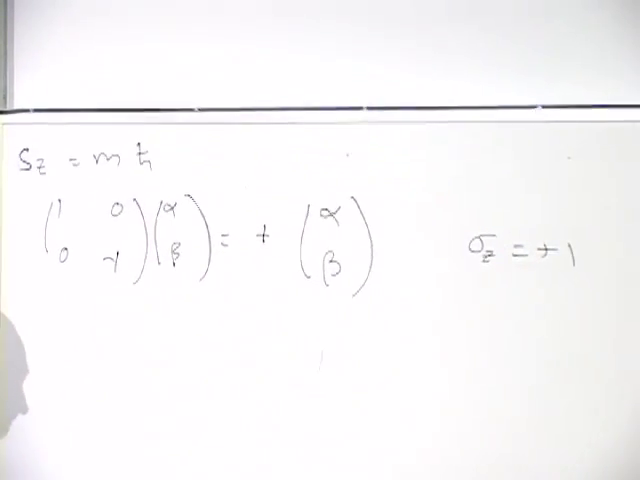
\includegraphics[width=0.74\textwidth]{lecture_08_figure_02.png}
\caption{Die Eigenwertgleichung zum Eigenwert \(+1\) für die Wirkung von \(\sigma_z\) auf einen Zweikomponentenspinor.}
\lectureframe{00:34:57}
\end{figure}

Zum Eigenwert \(+1\) ergibt die zeilenweise Multiplikation
\begin{equation}
\begin{pmatrix}
1\cdot\alpha+0\cdot\beta\\
0\cdot\alpha-\beta
\end{pmatrix}
=
\begin{pmatrix}
\alpha\\
-\beta
\end{pmatrix}
=
\begin{pmatrix}
\alpha\\
\beta
\end{pmatrix}.
\end{equation}
Die obere Gleichung ist automatisch erfüllt, während die untere \(-\beta=\beta\) und damit \(\beta=0\) liefert. Die Normierung verlangt \(|\alpha|=1\). Wählt man die irrelevante Gesamtphase so, dass \(\alpha=1\) gilt, erhält man
\begin{equation}
|+z\rangle=
\begin{pmatrix}
1\\
0
\end{pmatrix}.
\end{equation}

Zum Eigenwert \(-1\) gilt
\begin{equation}
\begin{pmatrix}
\alpha\\
-\beta
\end{pmatrix}
=
\begin{pmatrix}
-\alpha\\
-\beta
\end{pmatrix}.
\end{equation}
Nun ist die untere Gleichung automatisch erfüllt; die obere liefert \(\alpha=-\alpha\), also \(\alpha=0\). Mit der Wahl \(\beta=1\) ergibt sich
\begin{equation}
|-z\rangle=
\begin{pmatrix}
0\\
1
\end{pmatrix}.
\end{equation}

Ändern wir nun das Experiment und messen \(S_x\). Da
\begin{equation}
\sigma_x
\begin{pmatrix}
\alpha\\
\beta
\end{pmatrix}
=
\begin{pmatrix}
0\cdot\alpha+\beta\\
\alpha+0\cdot\beta
\end{pmatrix}
=
\begin{pmatrix}
\beta\\
\alpha
\end{pmatrix},
\end{equation}
lautet die Gleichung zum Eigenwert \(+1\)
\begin{equation}
\begin{pmatrix}
\beta\\
\alpha
\end{pmatrix}
=
\begin{pmatrix}
\alpha\\
\beta
\end{pmatrix}.
\end{equation}
Die beiden Komponentengleichungen \(\beta=\alpha\) und \(\alpha=\beta\) sind dieselbe Bedingung. Aus der Normierung folgt
\begin{equation}
2|\alpha|^2=1,
\end{equation}
Eine zweckmäßige Wahl ist daher
\begin{equation}
|+x\rangle
=
\frac{1}{\sqrt2}
\begin{pmatrix}
1\\
1
\end{pmatrix}.
\end{equation}

\begin{figure}[t]
\centering
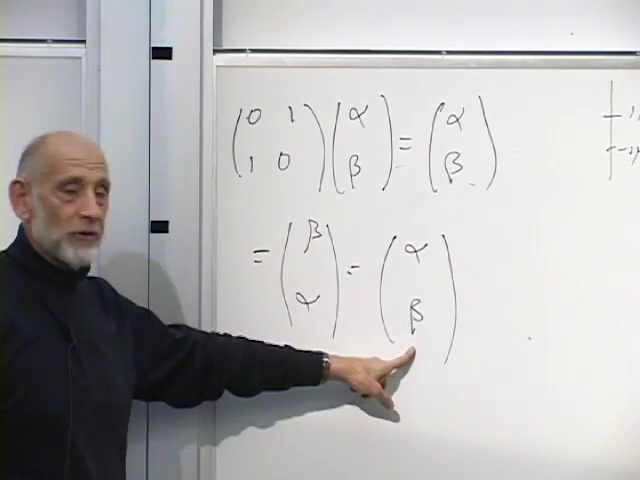
\includegraphics[width=0.74\textwidth]{lecture_08_figure_03.png}
\caption{Zum Eigenwert \(+1\) vertauscht \(\sigma_x\) die beiden Komponenten; daher muss \(\alpha=\beta\) gelten.}
\lectureframe{00:39:42}
\end{figure}

\begin{classroomqa}
\lecturetimestamp{00:40:13}
\audiencequestion{Wenn man den Faktor ein halb einbeziehen würde, wäre der Eigenwert dann ein halb?}
\lecturerresponse{Ja. Die Pauli-Matrix \(\sigma_x\) hat die Eigenwerte \(\pm1\), während \(S_x=\sigma_x/2\) die Eigenwerte \(\pm\tfrac12\) hat.}
\end{classroomqa}

Zum Eigenwert \(-1\) gilt
\begin{equation}
\begin{pmatrix}
\beta\\
\alpha
\end{pmatrix}
=
-
\begin{pmatrix}
\alpha\\
\beta
\end{pmatrix},
\end{equation}
also
\begin{equation}
\beta=-\alpha,
\qquad
\alpha=-\beta.
\end{equation}
Dies ist wiederum dieselbe Gleichung. Nach der Normierung gilt
\begin{equation}
|-x\rangle
=
\frac{1}{\sqrt2}
\begin{pmatrix}
1\\
-1
\end{pmatrix}.
\end{equation}
Eine gleichgewichtete Überlagerung der Zustände \(z\)-auf und \(z\)-ab ist somit entlang der positiven \(x\)-Achse polarisiert; dieselbe Überlagerung mit einem relativen Minuszeichen ist entlang der negativen \(x\)-Achse polarisiert.

Für die Richtung \(y\) gilt
\begin{equation}
\sigma_y
\begin{pmatrix}
\alpha\\
\beta
\end{pmatrix}
=
\begin{pmatrix}
-i\beta\\
i\alpha
\end{pmatrix}.
\end{equation}
Die beiden normierten Eigenvektoren sind
\begin{equation}
|+y\rangle
=
\frac{1}{\sqrt2}
\begin{pmatrix}
1\\
i
\end{pmatrix},
\qquad
|-y\rangle
=
\frac{1}{\sqrt2}
\begin{pmatrix}
1\\
-i
\end{pmatrix},
\end{equation}
bis auf eine Gesamtphase. Beide Zustände ergeben für \(z\)-auf die Wahrscheinlichkeit \(1/2\) und für \(z\)-ab die Wahrscheinlichkeit \(1/2\). Die relative Phase \(i\), die in diesen beiden Wahrscheinlichkeiten nicht sichtbar ist, unterscheidet die \(y\)- von der \(x\)-Polarisation. Linearkombinationen beschreiben auch Spinpolarisationen entlang beliebiger Richtungen; diese Rechnung wird auf später verschoben.

\begin{classroomqa}
\lecturetimestamp{00:44:22}
\audiencequestion{Wurde das Vorzeichen der \(i\)-Komponente dem falschen Eigenwert von \(\sigma_y\) zugeordnet?}
\lecturerresponse{Möglicherweise wurde das Vorzeichen tatsächlich dem falschen Eigenwert zugeordnet. Die Zuordnung ist hier unsicher; sie wird nicht aus dem Gedächtnis festgelegt.}
\end{classroomqa}

Die direkte Überprüfung lautet
\begin{align}
\sigma_y\frac{1}{\sqrt2}
\begin{pmatrix}
1\\
i
\end{pmatrix}
&=
\frac{1}{\sqrt2}
\begin{pmatrix}
-i\,i\\
i
\end{pmatrix}
=
\frac{1}{\sqrt2}
\begin{pmatrix}
1\\
i
\end{pmatrix},\\
\sigma_y\frac{1}{\sqrt2}
\begin{pmatrix}
1\\
-i
\end{pmatrix}
&=
\frac{1}{\sqrt2}
\begin{pmatrix}
(-i)(-i)\\
i
\end{pmatrix}
=
-\frac{1}{\sqrt2}
\begin{pmatrix}
1\\
-i
\end{pmatrix}.
\end{align}
Damit gehört \(+i\) zum Eigenwert \(+1\) und \(-i\) zum Eigenwert \(-1\).\footnote{Auch nach mehreren Korrekturen bleibt die mündliche Zuordnung ungeklärt; die hier gezeigten Vorzeichen ergeben sich aus der dargestellten Matrixmultiplikation.} Jeder Spin-ein-halb-Zustand, einschließlich jedes Zustands mit Polarisation entlang einer beliebigen Richtung, ist eine Linearkombination von \(|+z\rangle\) und \(|-z\rangle\).

\section{Spin eins und ortsabhängige Spinoren}

Für Spin \(1\) sind die möglichen Werte von \(S_z\) \(+1,0,-1\). Der Zustandsraum ist daher dreidimensional. Spin \(1\) ist ganzzahliger Spin und entspricht bosonischer Statistik. Gesucht sind drei \(3\times3\)-Matrizen, die dieselben Drehimpulskommutatoren erfüllen.

Eine Darstellung, die die drei Koordinatenrichtungen gleich behandelt, ist unten angegeben.\footnote{Das Vorzeichen von \(S_y\) ergibt sich aus der bei \(00{:}48{:}50\) sichtbaren Matrix und wird auch durch \([S_x,S_y]=iS_z\) festgelegt. Eine Umkehr dieses Vorzeichens würde den geforderten Kommutator umkehren.}
\begin{equation}
\begin{aligned}
S_x
&=
i
\begin{pmatrix}
0&0&0\\
0&0&1\\
0&-1&0
\end{pmatrix},
&
S_y
&=
i
\begin{pmatrix}
0&0&1\\
0&0&0\\
-1&0&0
\end{pmatrix},\\
S_z
&=
i
\begin{pmatrix}
0&1&0\\
-1&0&0\\
0&0&0
\end{pmatrix}.
\end{aligned}
\end{equation}
Jede Matrix ist \(i\) mal einer reellen antisymmetrischen Matrix. Jede enthält eine \(1\), eine \(-1\) sowie eine verschwindende Zeile und Spalte, die der jeweiligen Koordinate zugeordnet sind: die erste für \(S_x\), die zweite für \(S_y\) und die dritte für \(S_z\). Das ist eine nützliche Eselsbrücke. In dieser Darstellung ist \(S_z\) nicht diagonal.

Sei
\begin{equation}
v=
\begin{pmatrix}
\alpha\\
\beta\\
\gamma
\end{pmatrix}.
\end{equation}
Dann gilt
\begin{equation}
S_zv
=
\begin{pmatrix}
i\beta\\
-i\alpha\\
0
\end{pmatrix}.
\end{equation}
Zum Eigenwert \(+1\) gilt
\begin{equation}
i\beta=\alpha,
\qquad
-i\alpha=\beta,
\qquad
0=\gamma.
\end{equation}
Also \(\beta=-i\alpha\) und \(\gamma=0\). Aus der Normierung folgt \(2|\alpha|^2=1\), somit
\begin{equation}
|m=+1\rangle
=
\frac{1}{\sqrt2}
\begin{pmatrix}
1\\
-i\\
0
\end{pmatrix}.
\end{equation}
Zum Eigenwert \(-1\) gilt
\begin{equation}
i\beta=-\alpha,
\qquad
-i\alpha=-\beta,
\qquad
0=-\gamma,
\end{equation}
also \(\beta=i\alpha\), \(\gamma=0\) und
\begin{equation}
|m=-1\rangle
=
\frac{1}{\sqrt2}
\begin{pmatrix}
1\\
i\\
0
\end{pmatrix}.
\end{equation}
Schließlich ergibt die Gleichung zum Eigenwert null \(\alpha=\beta=0\), sodass \(\gamma\) beliebig bleibt. Die normierte Lösung lautet
\begin{equation}
|m=0\rangle
=
\begin{pmatrix}
0\\
0\\
1
\end{pmatrix}.
\end{equation}
Weitere Eigenwerte gibt es nicht: Diese drei Eigenvektoren spannen den dreidimensionalen Raum vollständig auf. Die Faktoren \(1/\sqrt2\) sind nicht bloß Zierde. Dieselben Koeffizienten gehen später in quantitative experimentelle Vorhersagen ein, wenn die Algebra auf den Isospin angewandt wird.

\begin{classroomqa}
\lecturetimestamp{00:54:10}
\audiencequestion{Wie sind die komplexen Einträge dieser Spin-eins-Eigenvektoren zu lesen?}
\lecturerresponse{Für \(m=+1\) lauten die Komponenten \(1/\sqrt2,-i/\sqrt2,0\), für \(m=-1\) lauten sie \(1/\sqrt2,i/\sqrt2,0\) und für \(m=0\) lauten sie \(0,0,1\).}
\end{classroomqa}

Andere Tripel von Matrizen erfüllen dieselbe Algebra und sind physikalisch gleichwertig. Die obige symmetrische Darstellung ist nützlich, weil sie alle drei Richtungen gleich behandelt; wir werden sie erneut verwenden.

\subsection{Ortsabhängigkeit wieder einführen}

Nun beziehen wir die Bewegung des Teilchens wieder ein. Der Spin kommutiert mit Position und Impuls, daher kann jeweils eine der beiden Größen zusammen mit einer Spin-Komponente festgelegt werden. Position und Impuls kommutieren nicht miteinander; auch verschiedene Spin-Komponenten kommutieren nicht miteinander.

Ein bewegtes Spin-ein-halb-Teilchen wird durch einen ortsabhängigen Spinor beschrieben:
\begin{equation}
\psi(x)=
\begin{pmatrix}
\psi_\uparrow(x)\\
\psi_\downarrow(x)
\end{pmatrix}.
\end{equation}
Die Größen
\begin{equation}
\rho_{\uparrow_z}(x)=|\psi_\uparrow(x)|^2,
\qquad
\rho_{\downarrow_z}(x)=|\psi_\downarrow(x)|^2
\end{equation}
sind gemeinsame Orts- und Spin-Wahrscheinlichkeitsdichten. Ihre Summe
\begin{equation}
\rho(x)=\psi^\dagger(x)\psi(x)
=|\psi_\uparrow(x)|^2+|\psi_\downarrow(x)|^2,
\end{equation}
ist die Ortsdichte. Ist bekannt, dass das Teilchen bei \(x\) nachgewiesen wurde, dann lauten die bedingten Wahrscheinlichkeiten
\begin{equation}
P(\uparrow_z\mid x)
=
\frac{|\psi_\uparrow(x)|^2}{\psi^\dagger(x)\psi(x)},
\qquad
P(\downarrow_z\mid x)
=
\frac{|\psi_\downarrow(x)|^2}{\psi^\dagger(x)\psi(x)},
\end{equation}
vorausgesetzt, \(\rho(x)\neq0\). Ein Elektron wird also durch eine räumliche Wellenfunktion mit zwei Komponenten beschrieben, deren lokale Spinamplituden sich von Ort zu Ort ändern können.

Für ein bewegtes Spin-eins-Teilchen schreiben wir
\begin{equation}
\phi(x)=
\begin{pmatrix}
\phi_1(x)\\
\phi_2(x)\\
\phi_3(x)
\end{pmatrix}.
\end{equation}
An jedem Raumpunkt bilden die drei Komponenten einen Vektor in demselben Spinraum wie zuvor. Teilchen mit Spin eins haben ganzzahligen Spin und sind Bosonen.

\begin{classroomqa}
\lecturetimestamp{01:00:10}
\audiencequestion{Ist \(\phi_1(x)\) selbst die Wahrscheinlichkeit für das Spin-eins-Ergebnis \(m=+1\)?}
\lecturerresponse{Nein. Es ist eine Amplitude in der gewählten dreikomponentigen Basis. Um ein bestimmtes Spinergebnis zu erhalten, bildet man das Bra des entsprechenden normierten Eigenvektors, projiziert das Feld darauf und nimmt den Betrag zum Quadrat.}
\end{classroomqa}

\begin{figure}[t]
\centering
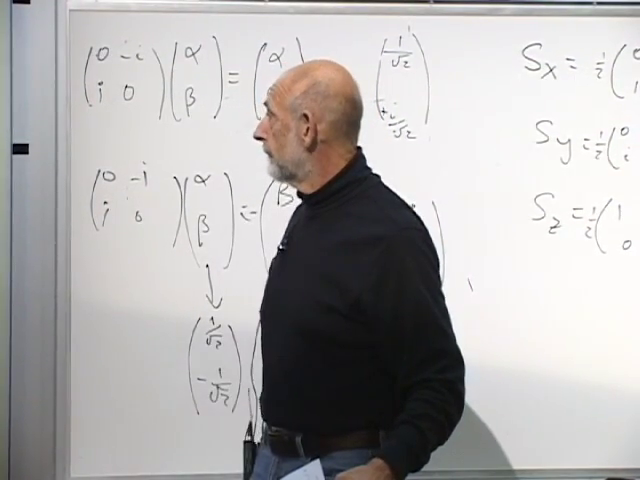
\includegraphics[width=0.82\textwidth]{lecture_08_figure_04.png}
\caption{Normierte Eigenvektoren von \(\sigma_y\) neben den drei Spin-ein-halb-Matrizen.}
\lectureframe{01:00:12}
\end{figure}

Zum Beispiel gilt
\begin{equation}
\begin{aligned}
|m=+1\rangle
&=
\frac{1}{\sqrt2}
\begin{pmatrix}
1\\
-i\\
0
\end{pmatrix}
\\
\Longrightarrow\quad\langle m=+1|
&=
\frac{1}{\sqrt2}
\begin{pmatrix}
1&i&0
\end{pmatrix}.
\end{aligned}
\end{equation}
Die Projektionsamplitude lautet daher
\begin{align}
\langle m=+1|\phi(x)\rangle
&=
\frac{1}{\sqrt2}
\begin{pmatrix}
1&i&0
\end{pmatrix}
\begin{pmatrix}
\phi_1(x)\\
\phi_2(x)\\
\phi_3(x)
\end{pmatrix}\\
&=
\frac{\phi_1(x)+i\phi_2(x)}{\sqrt2}.
\end{align}
Wendet man dieselbe Regel auf alle drei Eigenvektoren an, erhält man die spinaufgelösten Dichten.\footnote{Diese Formeln vervollständigen die Projektionsalgebra nach der ausdrücklichen Korrektur, dass \(\phi_1\) und \(\phi_2\) nicht reell sein müssen. Würde man sie als reell behandeln, ginge die Interferenz fälschlich verloren, die die Dichten für \(m=+1\) und \(m=-1\) unterscheidet.}
\begin{align}
\rho_{+1}(x)
&=
\frac12\left|\phi_1(x)+i\phi_2(x)\right|^2,\\
\rho_{-1}(x)
&=
\frac12\left|\phi_1(x)-i\phi_2(x)\right|^2,\\
\rho_0(x)
&=
|\phi_3(x)|^2.
\end{align}
Sie erfüllen
\begin{equation}
\begin{aligned}
\rho_{+1}(x)+\rho_{-1}(x)+\rho_0(x)
&=
|\phi_1(x)|^2+|\phi_2(x)|^2
\\
&\quad{}+|\phi_3(x)|^2
\\
&=
\phi^\dagger(x)\phi(x).
\end{aligned}
\end{equation}
Ist bekannt, dass das Teilchen bei \(x\) nachgewiesen wurde, dann gilt
\begin{equation}
P(m\mid x)
=
\frac{\rho_m(x)}{\phi^\dagger(x)\phi(x)},
\end{equation}
vorausgesetzt, \(\phi^\dagger(x)\phi(x)\neq0\). Die allgemeine Messregel ist stets dieselbe: Man bildet das Bra des gewünschten normierten Eigenvektors, projiziert den tatsächlichen Zustand darauf und nimmt den Betrag zum Quadrat. Die resultierende Dichte behält ihre Ortsabhängigkeit bei.

Matrizen für höhere Spins sind komplizierter, doch das Prinzip bleibt dasselbe.

\begin{classroomqa}
\lecturetimestamp{01:07:31}
\audiencequestion{Wie groß ist der Zustandsraum für Spin drei halbe?}
\lecturerresponse{Er umfasst vier Zustände mit \(m=\tfrac32,\tfrac12,-\tfrac12,-\tfrac32\). Spin zwei hat fünf Zustände.}
\end{classroomqa}

\begin{classroomqa}
\lecturetimestamp{01:07:55}
\audiencequestion{Warum umfasst die Diskussion \(x,y,z\), aber keine Zeitrichtung? Ist diese Behandlung nichtrelativistisch?}
\lecturerresponse{Bislang ist sie nichtrelativistisch. Spin lässt sich wie die Masse am einfachsten im Ruhesystem des Teilchens charakterisieren; seine Beschreibung in einem anderen Inertialsystem erhält man durch die entsprechende Lorentz-Transformation. Dieser relativistische Schritt wird auf später verschoben.}
\end{classroomqa}

Die Dirac-Gleichung liefert den relativistischen Rahmen und erklärt, warum ihre vierkomponentige Wellenfunktion ein Spin-Dublett enthält.

\section{Dirac-Matrizen und der vierkomponentige Spinor}

Die vierkomponentige Dirac-Wellenfunktion erfüllt
\begin{equation}
i\frac{\partial\Psi}{\partial t}
=
-i\alpha_i\frac{\partial\Psi}{\partial x_i}
+m\beta\Psi,
\qquad i=1,2,3,
\end{equation}
wobei über einen wiederholten räumlichen Index summiert wird. Der Ableitungsterm bedeutet also
\begin{equation}
\alpha_1\frac{\partial\Psi}{\partial x}
+\alpha_2\frac{\partial\Psi}{\partial y}
+\alpha_3\frac{\partial\Psi}{\partial z}.
\end{equation}
Für eine ebene Welle wird daraus die algebraische Gleichung
\begin{equation}
\omega\Psi=(\alpha_i k_i+m\beta)\Psi.
\end{equation}

\begin{classroomqa}
\lecturetimestamp{01:11:32}
\audiencequestion{Bezeichnen die beiden Vorkommen von \(m\) dasselbe?}
\lecturerresponse{Nein. Eines der beiden Vorkommen wurde als räumlicher Index verwendet, das andere bezeichnet die Masse des Teilchens. Benennen wir den räumlichen Index in \(i\) um; tritt \(i\) zweimal auf, wird von \(1\) bis \(3\) summiert.}
\end{classroomqa}

Das Quadrat des Frequenzoperators muss die relativistische Beziehung ergeben:
\begin{equation}
\omega^2=\mathbf{k}^2+m^2.
\end{equation}
Die quadratischen Terme verlangen daher für jedes \(i\)
\begin{equation}
\alpha_i^2=I_4,
\qquad
\beta^2=I_4.
\end{equation}

\begin{classroomqa}
\lecturetimestamp{01:13:01}
\audiencequestion{Ist \(\beta\) für jede der vier Komponenten von \(\Psi\) verschieden?}
\lecturerresponse{Nein. Es gibt eine Matrix \(\beta\), die auf den gesamten vierkomponentigen Spinor wirkt und \(\beta^2=I_4\) erfüllt.}
\end{classroomqa}

Die gemischten Terme müssen verschwinden. Für verschiedene räumliche Richtungen sowie zwischen jedem \(\alpha_i\) und \(\beta\) ergibt sich
\begin{equation}
\alpha_i\alpha_j+\alpha_j\alpha_i=0
\quad (i\neq j),
\qquad
\alpha_i\beta+\beta\alpha_i=0.
\end{equation}
Äquivalent dazu gilt
\begin{equation}
\{\alpha_i,\alpha_j\}=2\delta_{ij}I_4,
\quad
\{\alpha_i,\beta\}=0,
\quad
\{\beta,\beta\}=2I_4.
\end{equation}
Jede Matrix antikommutiert mit jeder anderen Matrix; ihr Antikommutator mit sich selbst ist dagegen das Doppelte der Einheitsmatrix.

Ohne \(\beta\) würden die drei Pauli-Matrizen bereits drei \(2\times2\)-Matrizen liefern, deren Quadrat die Einheitsmatrix ist und die paarweise antikommutieren. Der Massenterm verlangt eine vierte solche Matrix. Es gibt keine vierte \(2\times2\)-Matrix mit den geforderten Eigenschaften, und auch \(3\times3\)-Matrizen erfüllen die Algebra nicht. Die kleinste Darstellung ist daher \(4\times4\).

Eine \(4\times4\)-Matrix lässt sich in vier \(2\times2\)-Blöcke aufteilen. Eine zweckmäßige Darstellung ist
\begin{equation}
\alpha_i=
\begin{pmatrix}
\sigma_i&0\\
0&-\sigma_i
\end{pmatrix},
\qquad i=1,2,3.
\end{equation}

\begin{figure}[t]
\centering
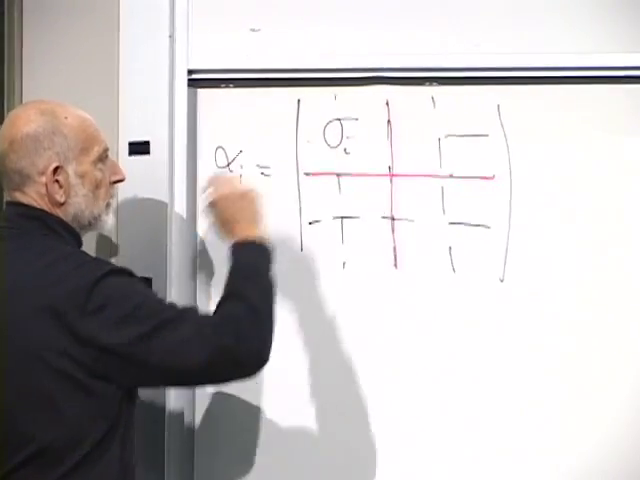
\includegraphics[width=0.68\textwidth]{lecture_08_figure_05.png}
\caption{Die Dirac-Matrix \(\alpha_i\) in \(2\times2\)-Blöcken, mit \(\sigma_i\) und \(-\sigma_i\) auf der Diagonalen.}
\lectureframe{01:17:23}
\end{figure}

\begin{classroomqa}
\lecturetimestamp{01:17:41}
\audiencequestion{Waren die \(\sigma_i\)-Blöcke in der früheren Darstellung anders angeordnet?}
\lecturerresponse{Ja. In einer anderen Darstellung standen sie außerhalb der Diagonalen. Die beiden Anordnungen sind äquivalent und durch eine Ähnlichkeitstransformation miteinander verbunden.}
\end{classroomqa}

In der vorliegenden Darstellung lautet die verbleibende Matrix
\begin{equation}
\beta=
\begin{pmatrix}
0&I_2\\
I_2&0
\end{pmatrix},
\qquad
I_2=
\begin{pmatrix}
1&0\\
0&1
\end{pmatrix}.
\end{equation}
Durch Blockmultiplikation lassen sich Überprüfungen der \(4\times4\)-Algebra auf gewöhnliche Multiplikationen von \(2\times2\)-Matrizen zurückführen.

\begin{classroomqa}
\lecturetimestamp{01:19:17}
\audiencequestion{Verwendete die frühere Darstellung ein anderes Vorzeichen oder eine Diagonalform für \(\beta\)?}
\lecturerresponse{Sie verwendete eine andere, aber physikalisch äquivalente Basis. Ein Basiswechsel mischt die vier Komponenten von \(\Psi\) und verändert das Aussehen der Matrizen, ohne die Physik zu ändern.}
\end{classroomqa}

Die vier Einträge von \(\Psi\) sind nicht die vier Raumzeitkoordinaten. Sie sind Koordinaten im kleinsten Vektorraum, auf dem diese Antikommutationsalgebra wirken kann. Es gibt zwei verschiedene Zweierstrukturen: die Aufteilung in \(2\times2\)-Blöcke und die Zweikomponenten-Pauli-Struktur innerhalb jedes Blocks. Der weiter unten begründeten Deutung vorgreifend lassen sich die vier Möglichkeiten wie folgt anordnen:
\begin{equation}
\begin{array}{c|cc}
& S_z=+\tfrac12 & S_z=-\tfrac12\\ \hline
\omega>0 & (\omega>0,+\tfrac12) & (\omega>0,-\tfrac12)\\
\omega<0 & (\omega<0,+\tfrac12) & (\omega<0,-\tfrac12)
\end{array}.
\end{equation}
Die untere Zeile besteht aus Elektronenzuständen mit negativer Frequenz. Sie ist keine Zeile von Positronen; ein Positron wird als Loch in der gefüllten Menge dieser Zustände gedeutet.

\section{Energieverdopplung im Ruhesystem und das Positron}

Die zweifache Energiestruktur lässt sich am einfachsten bei verschwindendem Impuls sichtbar machen. Wenn \(\mathbf{k}=0\), ist der Zustand der ebenen Welle räumlich konstant und der räumliche Ableitungsterm verschwindet. Die Gleichung im Ruhesystem\footnote{Der Frame bei \(01{:}23{:}38\) enthält auf dem Massenterm vorübergehend noch einen zusätzlichen Faktor \(i\); die mündliche Korrektur bei \(01{:}24{:}05\) entfernt ihn.} lautet
\begin{equation}
i\frac{\partial\Psi}{\partial t}=m\beta\Psi.
\end{equation}

\begin{figure}[t]
\centering
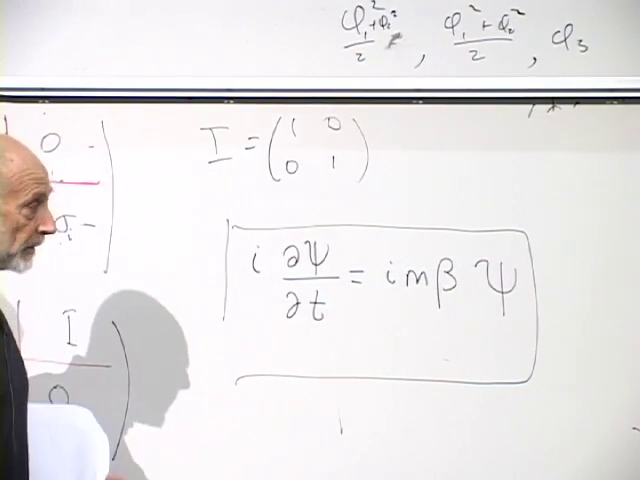
\includegraphics[width=0.76\textwidth]{lecture_08_figure_06.png}
\caption{Bei verschwindendem Impuls verschwinden die räumlichen Ableitungen; übrig bleibt die korrigierte Gleichung im Ruhesystem \(i\partial_t\Psi=m\beta\Psi\).}
\lectureframe{01:23:38}
\end{figure}

Teilen wir die vierkomponentige Spalte in ein oberes und ein unteres zweikomponentiges Objekt auf:
\begin{equation}
\Psi=
\begin{pmatrix}
\psi_+\\
\psi_-
\end{pmatrix}.
\end{equation}

\begin{classroomqa}
\lecturetimestamp{01:24:47}
\audiencequestion{Bedeuten die Bezeichnungen \(\psi_+\) und \(\psi_-\) bereits positive und negative Energie?}
\lecturerresponse{Nein. In diesem Stadium sind es lediglich Namen für den oberen und den unteren Zweikomponentenblock. Ihre Energiekombinationen wurden noch nicht bestimmt.}
\end{classroomqa}

\begin{classroomqa}
\lecturetimestamp{01:25:10}
\audiencequestion{Was stellt die aufgeteilte Spalte mit vier Komponenten dar?}
\lecturerresponse{Es ist derselbe vierkomponentige Dirac-Spinor, angeordnet passend zur Blockform der Matrizen. Jede Hälfte ist ein Objekt mit zwei Komponenten, und zusammen bilden die beiden Objekte die ursprüngliche Spalte mit vier Komponenten.}
\end{classroomqa}

Die Matrix \(\beta\) vertauscht die beiden Blöcke:
\begin{equation}
\beta
\begin{pmatrix}
\psi_+\\
\psi_-
\end{pmatrix}
=
\begin{pmatrix}
\psi_-\\
\psi_+
\end{pmatrix}.
\end{equation}
Damit wird die Gleichung im Ruhesystem zu
\begin{equation}
i\frac{\partial\psi_+}{\partial t}=m\psi_-,
\qquad
i\frac{\partial\psi_-}{\partial t}=m\psi_+.
\end{equation}

Es bieten sich zwei naheliegende Möglichkeiten an. Eine weitere Zeitableitung würde das System entkoppeln, aber durch Addieren und Subtrahieren der beiden Gleichungen wird es unmittelbar diagonalisiert. Tatsächlich gilt
\begin{align}
i\frac{\partial}{\partial t}(\psi_++\psi_-)
&=m(\psi_++\psi_-),\\
i\frac{\partial}{\partial t}(\psi_+-\psi_-)
&=-m(\psi_+-\psi_-).
\end{align}
Mit den Definitionen
\begin{equation}
\chi_+=\psi_++\psi_-,
\qquad
\chi_-=\psi_+-\psi_-,
\end{equation}
erhält man zwei voneinander unabhängige Gleichungen:
\begin{equation}
i\partial_t\chi_+=m\chi_+,
\qquad
i\partial_t\chi_-=-m\chi_-.
\end{equation}
Bei einer Frequenzabhängigkeit der Form \(e^{-i\omega t}\) gilt für die Summe
\begin{equation}
\omega=+m,
\end{equation}
während für die Differenz gilt
\begin{equation}
\omega=-m.
\end{equation}
Das ist genau die Aufspaltung in positive und negative Energie, die wir bereits im früheren eindimensionalen Beispiel gefunden haben: Auch die relativistische Gleichung besitzt Lösungen für Elektronen mit positiver und mit negativer Energie. Die Aufspaltung des Blocks führt also zu Zweigen positiver und negativer Energie. Zustände im reinen Ruhesystem lassen sich schreiben als
\begin{equation}
\Psi_{\omega=+m}=
\begin{pmatrix}
\xi\\
\xi
\end{pmatrix},
\qquad
\Psi_{\omega=-m}=
\begin{pmatrix}
\xi\\
-\xi
\end{pmatrix},
\end{equation}
wobei \(\xi\) weiterhin ein beliebiges Objekt mit zwei Komponenten ist.

Die Summe und die Differenz haben eine der beiden zweifachen Strukturen aufgelöst; die beiden Komponenten von \(\xi\) bleiben jedoch erhalten. Die Pauli-Matrizen wirken auf dieses verbleibende Komponentenpaar. Es ist das mit dem Spin verbundene Paar, was noch anhand von Drehungen und Erhaltungssätzen überprüft werden muss.

\begin{classroomqa}
\lecturetimestamp{01:32:23}
\audiencequestion{Kann man den Spin als äußere zweifache Struktur und das Vorzeichen der Energie als innere auffassen?}
\lecturerresponse{Ja. Die beiden Anordnungen der Faktoren sind gleichwertig. Man kann vertauschen, welcher Index zuerst geschrieben wird; dadurch werden lediglich die vier Komponenten umgeordnet.}
\end{classroomqa}

Der Zweig negativer Frequenz führt zur Interpretation des Dirac-Sees. Einer negativen Frequenz wird eine negative Elektronenenergie zugeordnet. Besetzt man alle Elektronenzustände mit negativer Energie, sinkt die Energie so weit, wie es das Ausschlussprinzip zulässt, denn jeder vollständige fermionische Zustand kann nur von einem Elektron besetzt werden. Das vollständig gefüllte negative Energie-See wird dann als Vakuum bezeichnet.

Man hebt ein Elektron aus diesem gefüllten See in einen Zustand positiver Energie. Das Ergebnis besteht aus einem Elektron mit positiver Energie und einem unbesetzten Zustand negativer Energie. Entfernt man eine negative Energie, steigt die Energie; das Loch hat daher eine positive Anregungsenergie. Da ein Elektron fehlt, trägt es außerdem die entgegengesetzte elektrische Ladung. Das Loch ist ein Positron.

\begin{classroomqa}
\lecturetimestamp{01:32:57}
\audiencequestion{Können Sie die Interpretation des Positrons noch einmal erklären?}
\lecturerresponse{Die Summe der beiden Blöcke hat eine positive Frequenz, die Differenz eine negative. Die Lösungen mit negativer Frequenz sind Elektronenzustände mit negativer Energie, und das Vakuum erhält man, indem man sie alle besetzt. Hebt man ein besetztes Elektron in einen Zustand positiver Energie, bleiben sowohl ein Elektron mit positiver Energie als auch ein Loch zurück. Dieses Loch mit positiver Energie und entgegengesetzter Ladung ist das Positron.}
\end{classroomqa}

Die Algebra hat somit zugleich zwei Folgen hervorgebracht: Zweige positiver und negativer Energie, aus denen die Teilchen--Antiteilchenstruktur entsteht, und eine verbleibende Zweikomponentenstruktur, die mit dem Spin eins halb verbunden ist. Bemerkenswert ist, dass beides aus den kleinsten Matrizen hervorging, die die relativistischen Antikommutationsrelationen erfüllen können. Der Spin war erst kurz zuvor als empirische Eigenschaft entdeckt worden, als diese mathematische Konstruktion Teilchen mit Spin und zugleich einen Antiteilchenzweig hervorbrachte; im damaligen historischen Kontext war das ein dramatisches Ergebnis.

\begin{classroomqa}
\lecturetimestamp{01:35:14}
\audiencequestion{Sind die Elektronen mit negativer Energie selbst Positronen?}
\lecturerresponse{Nein. Die Elektronenzustände mit negativer Energie sind im Vakuum besetzt. Ein Positron ist das Fehlen eines Elektrons in dieser besetzten Menge: ein Loch, kein Elektron mit negativer Energie.}
\end{classroomqa}

Ein Loch kann an Übergängen beteiligt sein. Ein Positron hat positive Energie, weil es dem Fehlen eines Elektrons mit negativer Energie entspricht. Füllt ein Elektron mit positiver Energie das Loch, annihilieren Elektron und Positron; ihre Energie muss jedoch abgeführt werden, gewöhnlich durch Photonen. In der Sprache des Dirac-Sees hat ein Elektron einen unbesetzten Zustand negativer Energie besetzt. Dieselbe Energiefreisetzung lässt sich als Übergang eines angeregten Elektrons in einem Atom auf ein niedrigeres Energieniveau veranschaulichen: Beim Übergang nach unten werden Photonen emittiert.

\begin{classroomqa}
\lecturetimestamp{01:36:39}
\audiencequestion{Warum fallen Elektronen mit höherer negativer Energie nicht in das Loch?}
\lecturerresponse{Diese Frage vermischt zwei Fälle. Wenn ein Elektron mit positiver Energie das Loch füllt, kommt es zur Elektron--Positron-Annihilation; Photonen tragen die Energie fort. Ein Übergang durch ein Elektron aus dem See mit negativer Energie ist ein anderer Prozess, der weiter unten behandelt wird.}
\end{classroomqa}

Die Rechnung für verschwindenden Impuls hat für sich genommen gezeigt, dass nach Abtrennung des Energievorzeichens eine zweifache Entartung verbleibt. Eine Entartung zweier Zustände ist für sich allein kein Beweis dafür, dass diese Zustände Drehimpuls tragen.

\begin{classroomqa}
\lecturetimestamp{01:37:44}
\audiencequestion{Wie beweist die Rechnung für verschwindenden Impuls, dass das verbleibende Zuständepaar den Spin darstellt?}
\lecturerresponse{Man kann das Paar als Spin-auf und Spin-ab bezeichnen, und in der vollständigen Gleichung treten die Pauli-Matrizen auf; das allein ist aber noch kein Beweis. Man muss entweder zeigen, wie sich das Paar unter räumlichen Drehungen transformiert, oder nachweisen, dass bei der Zuordnung eines Spins der Gesamtdrehimpuls in Wechselwirkungen und Stößen erhalten bleibt. Dieser Nachweis folgt später.}
\end{classroomqa}

Für einen Zustand positiver Energie im Ruhesystem sind der obere und der untere Block gleich:
\begin{equation}
\Psi_{\omega=+m}=
\begin{pmatrix}
\xi\\
\xi
\end{pmatrix}.
\end{equation}
Dass \(\xi\) ein Drehimpulsdublett bildet, muss durch das soeben beschriebene Drehungs- oder Erhaltungsargument nachgewiesen werden; es folgt nicht allein daraus, dass zwei Komponenten vorhanden sind.

\begin{classroomqa}
\lecturetimestamp{01:40:46}
\audiencequestion{Kann ein anderes Elektron mit dem Positron annihilieren, auch wenn es eine andere Energie hat?}
\lecturerresponse{Ja. Elektronen behalten keine individuelle Identität. Jedes verfügbare Elektron kann das Loch füllen; Unterschiede in der anfänglichen Energie und im anfänglichen Impuls spiegeln sich in Anzahl und Energien der emittierten Photonen wider.}
\end{classroomqa}

Das Lochbild erklärt auch einen Übergang, der vollständig innerhalb des negativen Energie-Sees abläuft. Angenommen, ein besetzter Zustand mit negativer Energie geht in das Loch über. Das ursprüngliche Loch wird gefüllt, aber der Zustand, aus dem dieses Elektron kam, ist nun leer. Das Loch hat sich verschoben. Gleichbedeutend damit hat das Positron seine Energie geändert und Strahlung emittiert.

\begin{classroomqa}
\lecturetimestamp{01:42:12}
\audiencequestion{Warum können benachbarte Energieniveaus mit negativer Energie nicht nacheinander in das Loch fallen?}
\lecturerresponse{Sie können das Loch von einem Niveau zu einem anderen verschieben. Ein Elektron, das in das ursprüngliche Loch fällt, hinterlässt an seiner vorherigen Energie ein neues Loch; so erhält das ursprüngliche Positron eine andere Energie. Die Energiedifferenz wird von Photonen fortgetragen.}
\end{classroomqa}

\begin{classroomqa}
\lecturetimestamp{01:44:39}
\audiencequestion{Warum führt dies nicht zu einer endlosen Strahlungskaskade zu immer niedrigeren Energien?}
\lecturerresponse{Weil Energie und Impuls gleichzeitig erhalten bleiben müssen. Diese beiden Erhaltungssätze lassen den uneingeschränkten Prozess nicht zu. Dasselbe gilt für ein gewöhnliches freies Elektron: Es kann nicht einfach im leeren Raum fortwährend seine Energie senken, indem es Photonen emittiert.}
\end{classroomqa}

\chapter{Lagrangedichten, Felder und lokale Teilchenprozesse}

Bosonenfelder, Fermionenfelder und das elektromagnetische Feld erfüllen wellenartige Gleichungen. Diese Gleichungen enthalten die Felder selbst sowie ihre räumlichen und zeitlichen Ableitungen. Man könnte für jedes Feld eine eigene Bewegungsgleichung angeben; eine Lagrangedichte fasst jedoch das gesamte System in einem kompakten Ausdruck zusammen. Wendet man auf diesen Ausdruck die Euler--Lagrange-Regel an, erhält man gleichzeitig die Gleichungen für alle Felder.

Diese Konstruktion hängt eng mit dem Prinzip der stationären Wirkung zusammen. Hier geht es zunächst um eine konkretere Aufgabe: herauszufinden, wovon eine Feld-Lagrangedichte abhängt, mit ihr einige klassische Gleichungen herzuleiten und dieselben Feldausdrücke anschließend quantenmechanisch neu zu deuten. In der Quantentheorie bestimmt die Lagrangedichte die Bewegung und Wechselwirkung von Teilchen und letztlich die Amplituden und Wirkungsquerschnitte bei Stößen.

\section{Ein kompakter Formalismus für Feldgleichungen}

Für ein einzelnes Skalarfeld hängt die Lagrangedichte vom Feld und seinen ersten Ableitungen ab,
\begin{equation}
\mathcal L
=
\mathcal L\!\left(\phi,\partial_t\phi,\partial_x\phi,\ldots\right)
=
\mathcal L\!\left(\phi,\partial_\mu\phi\right).
\end{equation}
Bei Rechnungen ist die explizite Auflistung der zeitlichen und räumlichen Ableitungen oft hilfreicher; die Schreibweise \(\partial_\mu\phi\) fasst dieselbe Liste relativistisch zusammen.

\begin{figure}[htbp]
\centering
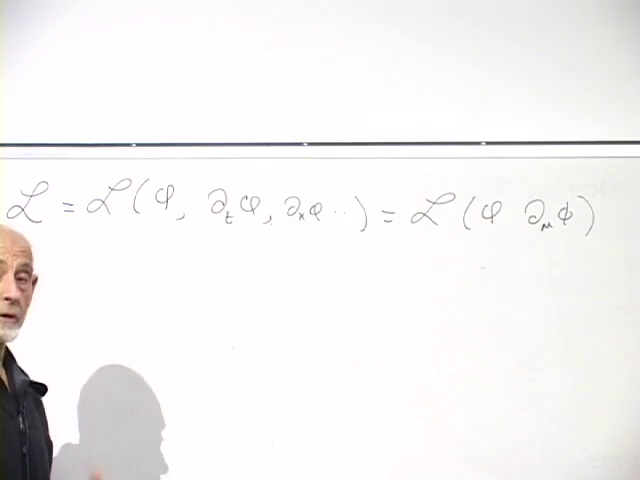
\includegraphics[width=0.82\textwidth]{lecture_09_figure_03.png}
\caption{Abhängigkeit einer Skalarfeld-Lagrangedichte vom Feld und seinen Raumzeit-Ableitungen.}
\lectureframe{00:03:56}
\end{figure}

Die Euler--Lagrange-Gleichung für Felder lautet
\begin{equation}
\frac{\partial}{\partial t}
\frac{\partial\mathcal L}{\partial\dot\phi}
+
\frac{\partial}{\partial x}
\frac{\partial\mathcal L}{\partial\phi_x}
+
\frac{\partial}{\partial y}
\frac{\partial\mathcal L}{\partial\phi_y}
+
\frac{\partial}{\partial z}
\frac{\partial\mathcal L}{\partial\phi_z}
=
\frac{\partial\mathcal L}{\partial\phi},
\end{equation}
wobei
\begin{equation}
\dot\phi=\frac{\partial\phi}{\partial t},
\qquad
\phi_x=\frac{\partial\phi}{\partial x},
\qquad
\phi_y=\frac{\partial\phi}{\partial y},
\qquad
\phi_z=\frac{\partial\phi}{\partial z}.
\end{equation}
Wenn \(\mathcal L\) mehrere Felder enthält, wird diese Regel für jedes Feld einzeln angewendet. Das Ergebnis ist das System der Bewegungsgleichungen.

Das einfachste Beispiel für ein Skalarfeld ist
\begin{equation}
\begin{split}
\mathcal L
&=
\frac12\dot\phi^2
-\frac12\phi_x^2
-\frac12\phi_y^2
-\frac12\phi_z^2
-V(\phi)
\\
&=
\frac12\dot\phi^2-\frac12(\boldsymbol\nabla\phi)^2-V(\phi).
\end{split}
\end{equation}
Die Terme mit räumlichen Ableitungen haben das entgegengesetzte Vorzeichen wie der Term mit der zeitlichen Ableitung. Leitet man die einzelnen Terme ab, erhält man
\begin{align}
\frac{\partial\mathcal L}{\partial\dot\phi}&=\dot\phi,
&
\frac{\partial\mathcal L}{\partial\phi_i}&=-\phi_i,
&
\frac{\partial\mathcal L}{\partial\phi}&=-V'(\phi),
\end{align}
und damit
\begin{equation}
\ddot\phi-\nabla^2\phi=-V'(\phi).
\end{equation}

\begin{figure}[htbp]
\centering
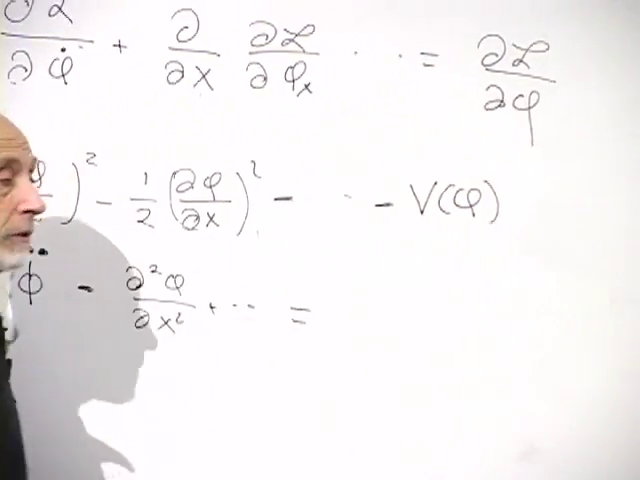
\includegraphics[width=0.74\textwidth]{lecture_09_figure_04.png}
\caption{Euler--Lagrange-Gleichung, Skalarfeld-Lagrangedichte und die von \(V(\phi)\) erzeugte Feldgleichung.}
\lectureframe{00:08:23}
\end{figure}

Dies ist die von der Skalarfeld-Lagrangedichte erzeugte Gleichung.\editorialnote{Der erhaltene Bildausschnitt ist am linken Rand abgeschnitten; die gezeigte Ergänzung ergibt sich eindeutig aus der unmittelbar vorausgehenden und anschließenden Herleitung.}

Hier ist \(V(\phi)\) die potenzielle Energiedichte des Feldes. Ein konstanter Beitrag zu \(V\) hat keinen Einfluss auf diese Gleichung, weil seine Ableitung verschwindet. Ein lineares Potential ist algebraisch möglich, hat aber keine untere Schranke: Die Feldenergie kann gegen minus unendlich gehen. Das erste stabile Beispiel ist daher
\begin{equation}
V(\phi)=\frac12m^2\phi^2,
\qquad
V'(\phi)=m^2\phi,
\end{equation}
woraus folgt
\begin{equation}
\ddot\phi-\nabla^2\phi=-m^2\phi.
\end{equation}

Um die Bedeutung von \(m\) sichtbar zu machen, setzen wir eine ebene Welle ein:
\begin{equation}
\phi(\mathbf x,t)=\phi_0e^{i\omega t-i\mathbf k\cdot\mathbf x}.
\end{equation}
Dann gilt
\begin{equation}
\ddot\phi=-\omega^2\phi,
\qquad
\nabla^2\phi=-\mathbf k^2\phi,
\end{equation}
sodass die Wellengleichung zu
\begin{equation}
-\omega^2\phi+\mathbf k^2\phi=-m^2\phi.
\end{equation}
wird. Nach dem Kürzen von \(\phi\) gilt
\begin{equation}
\omega^2=\mathbf k^2+m^2.
\end{equation}
In Einheiten mit \(\hbar=c=1\) sind Frequenz und Energie sowie Wellenzahl und Impuls gleich. Somit gilt
\begin{equation}
E^2=\mathbf p^2+m^2,
\end{equation}
oder, mit wieder eingesetzten Potenzen von \(c\), \(E^2=\mathbf p^2c^2+m^2c^4\). Der Parameter \(m\) ist die Masse eines Quants des Feldes.

Lorentz-Invarianz lässt sich bereits auf der Ebene des kompakten Ausdrucks sicherstellen. Ist \(\mathcal L\) ein Lorentz-Skalar, so sind seine Bewegungsgleichungen Lorentz-invariant. Das relative Vorzeichen zwischen zeitlichen und räumlichen Ableitungen entspricht dem vertrauten Raumzeit-Vorzeichen der speziellen Relativitätstheorie.

\section{Nichtlinearität und gekoppelte klassische Felder}

Höhere Potenzen eines Feldes führen zu einer neuen Art von Verhalten. Ist
\begin{equation}
V(\phi)=\frac12m^2\phi^2+g\phi^3,
\end{equation}
so gilt
\begin{equation}
\ddot\phi-\nabla^2\phi=-m^2\phi-3g\phi^2.
\end{equation}
Quadratische Terme in der Lagrangedichte ergeben lineare Gleichungen für das Feld. Kubische und höhere Terme führen zu nichtlinearen Gleichungen.

Der Unterschied zeigt sich in der Bewegung von Wellenpaketen. Bei einer linearen Gleichung lassen sich ein nach rechts und ein nach links laufendes Wellenpaket addieren, sodass eine weitere Lösung entsteht. Die Pakete überlagern sich eine Zeit lang und interferieren, durchdringen einander dann und laufen in ihrer ursprünglichen Form weiter. Bei nichtlinearen Termen beeinflussen sich die Pakete gegenseitig. Sie können gestreut oder verformt werden oder in kompliziertere Wellen zerfallen. Die vorübergehende Interferenz linearer Wellen ist keine Wechselwirkung; eine bleibende Veränderung der Pakete ist ein Zeichen für Nichtlinearität.

Dasselbe Muster tritt bei zwei Skalarfeldern auf. Sei
\begin{align}
\mathcal L
&=
\frac12(\partial_\mu\phi)(\partial^\mu\phi)
+\frac12(\partial_\mu\rho)(\partial^\mu\rho)
-V(\phi,\rho),
\\
V(\phi,\rho)
&=
\frac12m^2\phi^2+\frac12M^2\rho^2+\rho\phi^2.
\end{align}
Ohne den letzten Term sind die beiden Gleichungen unabhängig voneinander:
\begin{equation}
\ddot\phi-\nabla^2\phi=-m^2\phi,
\qquad
\ddot\rho-\nabla^2\rho=-M^2\rho.
\end{equation}
Sie beschreiben Quanten zweier Teilchensorten mit den Massen \(m\) und \(M\). Nimmt man den gemischten Term hinzu, gilt
\begin{align}
\ddot\phi-\nabla^2\phi&=-m^2\phi-2\rho\phi,
\\
\ddot\rho-\nabla^2\rho&=-M^2\rho-\phi^2.
\end{align}
Nun enthält jede Gleichung auch das jeweils andere Feld. Die Gleichungen sind gekoppelt und nichtlinear: Ein \(\phi\)-Paket streut ein \(\rho\)-Paket und umgekehrt. Die Ableitungsterme bestimmen die Energie--Impuls-Beziehung, die undifferenzierten quadratischen Terme legen die Massen fest und der gemischte Term höherer Ordnung beschreibt die Wechselwirkung. Das ist das grundlegende klassische Muster.

\section{Dirac-Felder und eine Skalarfeldkopplung}

Für ein Dirac-Feld ist die Gleichung erster Ordnung in der Zeit. In einer Kurzschreibweise für eine Dimension, wobei die Verallgemeinerung auf drei räumliche Richtungen vorausgesetzt wird, hat sie folgende Termstruktur:
\begin{equation}
i\dot\Psi
\simeq
i\alpha\frac{\partial\Psi}{\partial x}+m\beta\Psi,
\qquad
i\boldsymbol\alpha\cdot\boldsymbol\nabla\Psi
=i\sum_i\alpha_i\frac{\partial\Psi}{\partial x_i}.
\end{equation}
Die Matrizen \(\alpha_i\) und \(\beta\) wirken auf die Komponenten von \(\Psi\). Eine entsprechende Lagrangedichte enthält einen Term, der linear in \(\partial_t\Psi\) ist, ein Bilinear mit räumlicher Ableitung, an dem \(\alpha_i\) beteiligt ist, und das Massenbilinear \(m\Psi^\dagger\beta\Psi\). Hier benötigen wir nur diese strukturelle Aussage.\editorialnote{Die Vorzeichen, Klammern und die Stellung von \(i\) in der versuchsweise angegebenen Dirac-Lagrangedichte sind in der Vorlage ausdrücklich nicht festgelegt. Daraus wird keine exakte, von Konventionen abhängige Formel abgeleitet.}

\begin{figure}[htbp]
\centering
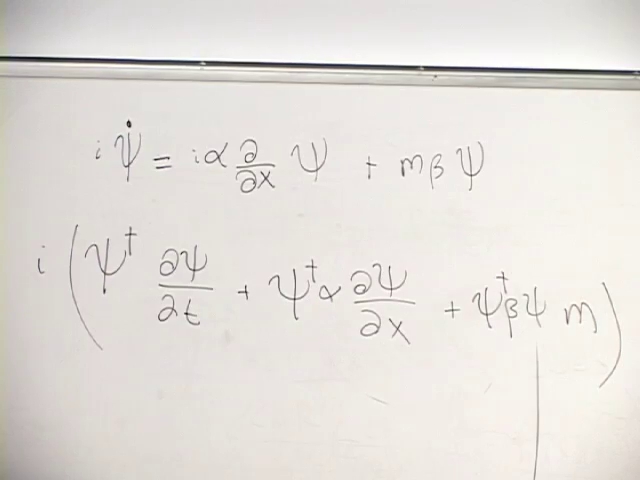
\includegraphics[width=0.76\textwidth]{lecture_09_figure_05.png}
\caption{Terme mit zeitlicher und räumlicher Ableitung sowie der Massenterm in der Diskussion des Dirac-Feldes.}
\lectureframe{00:25:37}
\end{figure}

\begin{classroomqa}
\lecturetimestamp{00:26:37}
\audiencequestion{Ist die Klammer in der versuchsweise angegebenen Dirac-Lagrangedichte richtig gesetzt, sodass \(i\) den gesamten Ausdruck multipliziert?}
\lecturerresponse{Die genaue Stellung wird hier nicht mit Sicherheit festgelegt und ist für den strukturellen Punkt auch nicht erforderlich: Es gibt eine Lagrangedichte, aus der die Dirac-Gleichung folgt.}
\end{classroomqa}

Fügen wir nun ein Skalarfeld \(\phi\) hinzu. Das naive Produkt \(\Psi^\dagger\Psi\,\phi\) ist kein Lorentz-Skalar. Setzt man stattdessen dieselbe Dirac-Matrix ein, die auch im Massenterm vorkommt, erhält man
\begin{equation}
\mathcal L_{\mathrm{int}}
\propto
\Psi^\dagger\beta\Psi\,\phi.
\end{equation}
Äquivalent dazu ist \(\Psi^\dagger\beta\Psi\) das skalare Dirac-Bilinear. Die Variation der vollständigen Lagrangedichte fügt der Dirac-Gleichung einen zu \(\phi\) proportionalen Term und der Skalarfeldgleichung eine zu \(\Psi^\dagger\beta\Psi\) proportionale Quelle hinzu. Die beiden Felder streuen einander.

\begin{classroomqa}
\lecturetimestamp{00:28:03}
\audiencequestion{Ist das in die Skalar--Fermion-Wechselwirkung eingesetzte \(\beta\) dasselbe \(\beta\), das auch im Dirac-Massenterm vorkommt?}
\lecturerresponse{Ja. Es ist dieselbe Dirac-Matrix.}
\end{classroomqa}

Der Vergleich
\begin{equation}
m\Psi^\dagger\beta\Psi
\qquad\hbox{and}\qquad
\Psi^\dagger\beta\Psi\,\phi
\end{equation}
lässt die Kopplung wie einen Massenparameter erscheinen, der durch ein Skalarfeld ersetzt wurde. Auf diese Beobachtung kommen wir gegen Ende zurück, wenn wir ein Feld mit einem von null verschiedenen Vakuumwert betrachten.

Bis hierher war die Deutung klassisch: Wellenpakete streuen andere Wellenpakete. Dieselbe Algebra erhält eine präzisere Teilchenbedeutung, wenn die Felder zu Operatoren werden.

\section{Was die Potenzen von Quantenfeldern bewirken}

Ein reelles Skalar-Quantenfeld enthält sowohl Erzeugungs- als auch Vernichtungsoperatoren. Schematisch gilt
\begin{equation}
\phi(x)\sim A^+(x)+A^-(x),
\end{equation}
wobei \(A^+\) ein Quant erzeugt und \(A^-\) eines vernichtet. Daher umfasst \(\phi^3(x)\) vier Arten lokaler Prozesse:
\begin{equation}
\phi^3
\sim
(A^+)^3+(A^+)^2A^-+A^+(A^-)^2+(A^-)^3,
\end{equation}
wobei in dieser schematischen Betrachtung die Details der Operatorreihenfolge und numerische Koeffizienten unterdrückt sind. Die vier Änderungen der Teilchenzahl lauten
\begin{equation}
3\longrightarrow0,
\qquad
0\longrightarrow3,
\qquad
2\longrightarrow1,
\qquad
1\longrightarrow2.
\end{equation}
Alle drei Feldfaktoren wirken am selben Punkt \(x\). Ein einzelner kubischer Term umfasst somit die Vernichtung dreier Teilchen, die Erzeugung dreier Teilchen, die Fusion zweier Quanten zu einem und die Aufspaltung eines Quants in zwei. In einer physikalischen Amplitude können einige dieser lokalen Deutungen später durch Energie--Impuls-Erhaltung ausgeschlossen werden; sie sind jedoch alle im Operatorprodukt selbst enthalten.

Die quadratischen freien Terme haben eine andere Funktion. Unterdrücken wir zunächst die Normierung des Unterschieds zwischen benachbarten Punkten \(x\) und \(x'\):
\begin{equation}
\partial_x\phi
\ \propto\
\phi(x)-\phi(x').
\end{equation}
Quadrieren und Ausmultiplizieren ergibt folgende Termstruktur:
\begin{align}
\frac12(\partial_x\phi)^2
&\ \propto\
\frac12\bigl[\phi(x)-\phi(x')\bigr]^2
\\
&=
\frac12\phi(x)^2
+\frac12\phi(x')^2
-\phi(x)\phi(x').
\end{align}
Jedes Quadrat an einem einzelnen Punkt lässt mehrere Operator-Deutungen zu: Es kann zwei Quanten erzeugen, zwei vernichten oder am selben Punkt eines vernichten und wieder erzeugen. Diese Terme transportieren kein Teilchen. Der gemischte Term kann ein Quant bei \(x'\) vernichten und eines bei \(x\) erzeugen oder umgekehrt. Er wirkt daher wie ein Hüpfterm zwischen nächsten Nachbarn. Wiederholte Faktoren transportieren ein Teilchen von \(x\) nach \(x'\), dann nach \(x''\) und so weiter. Quadratische Ableitungsterme bestimmen die freie Ausbreitung; kubische und höhere Terme streuen, erzeugen und vernichten Teilchen.

\begin{classroomqa}
\lecturetimestamp{00:36:07}
\audiencequestion{Muss die Differenzdarstellung der Ableitung den Abstand \(x-x'\) enthalten?}
\lecturerresponse{Ja. Bezeichnet man den Abstand mit \(L\), ergibt das Quadrieren der Differenz den Faktor \(L^{-2}\). Dieser Zahlenfaktor ändert den Koeffizienten, aber nichts an der Deutung als Hüpfterm.}
\end{classroomqa}

Mit wieder eingesetztem Abstand ergibt sich
\begin{align}
\frac12(\partial_x\phi)^2
&\longrightarrow
\frac{1}{2L^2}\bigl[\phi(x)-\phi(x')\bigr]^2
\\
&=
\frac{1}{2L^2}\phi(x)^2
+\frac{1}{2L^2}\phi(x')^2
-\frac{1}{L^2}\phi(x)\phi(x').
\end{align}

Auch der Massenterm ist quadratisch, enthält aber keine Ableitung:
\begin{equation}
\frac12m^2\phi(x)^2.
\end{equation}
In der Einteilchen-Deutung wird ein ankommendes Quant am selben Punkt absorbiert und wieder emittiert. Es bewegt das Quant nicht, sondern gewichtet – oder zählt in diesem Sinn – dessen Anwesenheit dort. Dasselbe Operatorquadrat enthält auch die Deutungen mit zwei Erzeugungen und mit zwei Vernichtungen. Für die Bewegung ist also entscheidend, ob ein gemischter Term benachbarte Punkte verbindet oder eine Masseneinfügung innerhalb eines Punktes wirkt.

\section{Der lokale Vertex der Quantenelektrodynamik}

Diese elementaren Skizzen von Teilchenprozessen bilden den Anfang der Feynman-Diagramme. Das zentrale Beispiel ist die Quantenelektrodynamik, die Theorie der Elektronen, Positronen und Photonen.

Die Dirac-Gleichung besitzt Moden mit positiver und negativer Energie. In der älteren Sprache enthält \(\Psi\) Vernichtungsoperatoren für beide Arten von Moden, während \(\Psi^\dagger\) die entsprechenden Erzeugungsoperatoren enthält. Die Entfernung eines Elektrons mit negativer Energie wird als Erzeugung eines Positrons mit positiver Energie umgedeutet. Nach dieser Umbenennung lautet die nützliche schematische Zerlegung
\begin{align}
\Psi
&\sim
C^-_{e^-}+C^+_{e^+},
\\
\Psi^\dagger
&\sim
C^+_{e^-}+C^-_{e^+}.
\end{align}
Somit vernichtet \(\Psi\) ein Elektron oder erzeugt ein Positron, während \(\Psi^\dagger\) ein Elektron erzeugt oder ein Positron vernichtet. Diese Kurzschreibweise enthält weder Normierung noch Spinindex oder Impulsintegral.

Die QED-Wechselwirkung koppelt den Dirac-Strom an das elektromagnetische Viererpotential. In der hier verwendeten Komponenten-Schreibweise hat sie folgende Struktur:
\begin{equation}
\mathcal L_{\mathrm{QED,int}}
\sim
e\left(
\Psi^\dagger\Psi\,A_0
+
\Psi^\dagger\boldsymbol{\alpha}\Psi\mathbin{\boldsymbol{\cdot}}\mathbf A
\right),
\end{equation}
wobei
\begin{equation}
J^0=\Psi^\dagger\Psi,
\qquad
\mathbf J=\Psi^\dagger\boldsymbol{\alpha}\Psi.
\end{equation}
Das Symbol \(\sim\) ist wichtig: Das relative Vorzeichen zwischen zeitlichem und räumlichem Term hängt von der Metrik- und Viererpotential-Konvention ab. Die invariante Aussage lautet, dass der Viererstrom mit dem Viererpotential kontrahiert wird.\editorialnote{Die Vorlage legt die zeitliche und räumliche Komponente des Stroms fest, bestimmt aber keine Metrik-Konvention für die Kontraktion der Komponenten.}

Das Photonenfeld \(A_\mu\) selbst enthält Erzeugungs- und Vernichtungsoperatoren für Photonen. Sein Vektorcharakter trägt außerdem die Polarisation des Photons--- – eine kleine Richtungs``markierung'' zusätzlich zu seinem Impuls.

\begin{classroomqa}
\lecturetimestamp{00:44:28}
\audiencequestion{Wie kann die Wechselwirkung ein Skalar sein, wenn \(A_\mu\) ein Vektor ist und der Fermionfaktor zunächst wie ein Skalar aussieht?}
\lecturerresponse{Auch die Fermionen liefern einen Vierervektor: \(\Psi^\dagger\Psi\) ist seine zeitliche Komponente und \(\Psi^\dagger\boldsymbol\alpha\Psi\) seine räumliche Komponente. Die Kontraktion dieses Stroms mit \(A_\mu\) ergibt einen Skalar.}
\end{classroomqa}

Multipliziert man die Operatorinhalte von \(\Psi^\dagger\), \(\Psi\) und \(A_\mu\), ergeben sich vier vertraute Deutungen eines lokalen Vertex:
\begin{enumerate}
\item Ein Elektron emittiert ein Photon;
\item ein Elektron absorbiert ein Photon;
\item ein Elektron und ein Positron annihilieren zu einem Photon;
\item ein Photon erzeugt ein Elektron--Positron-Paar.
\end{enumerate}
Bei der ersten Deutung vernichtet \(\Psi\) das einlaufende Elektron, \(\Psi^\dagger\) erzeugt das auslaufende Elektron und das Photonenfeld erzeugt das Photon. Wählt man den Vernichtungsanteil des Photons, erhält man die Absorption. Wählt man die Positron-Anteile, erhält man Paarvernichtung oder Paarerzeugung. Ein lokaler Term enthält die ganze Familie.

In einem Diagramm mit Fermionfluss zeigt der Pfeil auf einer Positronlinie entgegen der Ausbreitungsrichtung des Positrons. Bei dieser Konvention läuft der Fermionpfeil stetig durch jeden zulässigen QED-Vertex. Die vier Deutungen unterscheiden sich dadurch, dass äußere Linien zwischen der einlaufenden und der auslaufenden Seite verschoben werden, nicht dadurch, dass die Fermionflusslinie unterbrochen wird.

Jede dieser Deutungen trägt denselben Koeffizienten \(e\), die elektrische Ladung in der hier verwendeten mikroskopischen Konvention. Dieser Koeffizient ist die elektrische Ladung \(e\), nicht die Feinstrukturkonstante, obwohl beide eng zusammenhängen. Die Vertexamplitude ist proportional zu \(e\); berücksichtigt man alle kinematischen und Normierungsfaktoren, ist die entsprechende Wahrscheinlichkeit proportional zu \(e^2\).

\begin{classroomqa}
\lecturetimestamp{00:49:44}
\audiencequestion{Hat die Deutung Photon zu Elektron--Positron denselben Koeffizienten wie die anderen Deutungen des Vertex?}
\lecturerresponse{Ja. Sie enthält denselben Koeffizienten für die elektrische Ladung \(e\).}
\end{classroomqa}

\begin{classroomqa}
\lecturetimestamp{00:49:59}
\audiencequestion{Muss es einen Skalierungsfaktor geben, da eine Wahrscheinlichkeit keine Einheit hat?}
\lecturerresponse{In der hier verwendeten natürlichen mikroskopischen Konvention ist die Ladung \(e\) dimensionslos. Sie bestimmt die Größenordnung der Amplitude, ihr Quadrat die Größenordnung der Wahrscheinlichkeit.}
\end{classroomqa}

Ein konkretes Bild: Ein Elektron trifft auf eine Wand und kommt abrupt zum Stillstand. Mit einer gewissen Wahrscheinlichkeit werden Energie und Impuls in Form eines Photons abgegeben. Der elementare elektromagnetische Faktor in der Strahlungsamplitude ist \(e\); daher enthält die entsprechende Wahrscheinlichkeit \(e^2\). Diese Aussage isoliert den Kopplungsfaktor; die tatsächliche Wahrscheinlichkeit hängt auch vom Zustand des Elektrons und von der Kinematik ab.

\begin{figure}[htbp]
\centering
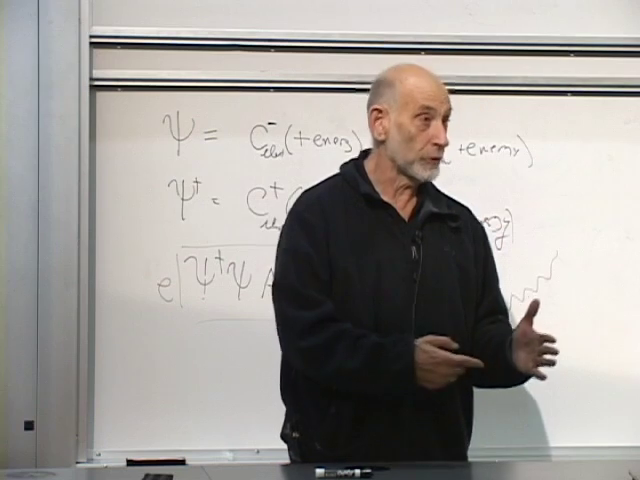
\includegraphics[width=0.78\textwidth]{lecture_09_figure_06.png}
\caption{Operatorinhalt von \(\Psi\) und \(\Psi^\dagger\) für Elektronen und Positronen sowie eine Skizze der Elektron--Photon-Wechselwirkung.}
\lectureframe{00:50:39}
\end{figure}

\begin{classroomqa}
\lecturetimestamp{00:51:15}
\audiencequestion{Hat die elektrische Ladung eine Einheit?}
\lecturerresponse{In der hier verwendeten natürlichen mikroskopischen Konvention nicht. Makroskopische Ladung wird oft in Coulomb angegeben, aber in der Teilchentheorie misst man die Ladung relativ zu einer gewählten elementaren Einheit. In Planck-Einheiten oder anderen natürlichen Einheiten werden die Größen als reine Zahlen ausgedrückt.}
\end{classroomqa}

Der Unterschied beruht auf Konventionen und Maßstäben. Coulomb eignet sich zur Angabe des Stroms in Leitungen; eine dimensionslose Kopplung ist für mikroskopische Amplituden praktisch.\editorialnote{Eine kurze Frage bei 00:52:37--00:53:15 zur ``Gruppierung'' ladungstragender Terme ist stark beschädigt und führte zu keiner eindeutigen Konstruktion.}

Alle drei Felder der elementaren QED-Wechselwirkung werden am selben Raumzeitpunkt ausgewertet. Dem Vertex selbst ist keine interne Zeitverzögerung zugeordnet.

\begin{classroomqa}
\lecturetimestamp{00:53:19}
\audiencequestion{Finden die Absorption und Wiederaussendung des Elektrons sowie die Emission des Photons gleichzeitig statt, oder enthält die Gleichung eine Verzögerung?}
\lecturerresponse{Am elementaren Vertex werden alle Operatoren am selben Raumzeitpunkt ausgewertet. Der grundlegende Prozess enthält daher keine Verzögerung zwischen diesen Vorgängen.}
\end{classroomqa}

\begin{classroomqa}
\lecturetimestamp{00:53:57}
\audiencequestion{Muss jede Erhaltungsgröße einzeln erhalten bleiben?}
\lecturerresponse{Ja. Die elektrische Ladung ist eine der Größen, die einzeln erhalten bleiben müssen.}
\end{classroomqa}

Die Ladungserhaltung ist sowohl im Diagramm als auch in der Algebra zu erkennen. Ein Prozess, der ein einlaufendes Elektron in ein auslaufendes Positron umwandelt, würde die Ladung umkehren und ist kein zulässiger QED-Vertex. Ist die Zeit nach oben aufgetragen, weist der Elektronenpfeil nach oben und der Positronenpfeil nach unten; am zulässigen Vertex verläuft immer ein Fermionpfeil durchgehend. Algebraisch enthält die Wechselwirkung ein \(\Psi\) und ein \(\Psi^\dagger\). Der erste erhöht die Ladung um eine Einheit, wenn er ein Elektron vernichtet oder ein Positron erzeugt; der zweite senkt sie um eine Einheit. Die Wirkungen heben sich auf.

\begin{classroomqa}
\lecturetimestamp{00:56:05}
\audiencequestion{Ist der eingerahmte Ausdruck für Elektron--Photon die gesamte QED-Lagrangedichte?}
\lecturerresponse{Nein. Es ist der Wechselwirkungsterm. Die quadratischen freien Photonenterme und die quadratischen Dirac-Terme, die die Ausbreitung bestimmen, sind nicht angegeben.}
\end{classroomqa}

\begin{classroomqa}
\lecturetimestamp{00:56:35}
\audiencequestion{Wird eine klassische Lagrangedichte hergeleitet, während man eine Quantен-Lagrangedichte errät und überprüft, und bleibt die Struktur kinetische Energie minus potenzielle Energie in der Quantenmechanik erhalten?}
\lecturerresponse{Das Muster kinetische Energie minus potenzielle Energie bleibt erhalten: Zeitliche Ableitungen liefern die kinetische Form, räumliche Gradienten verallgemeinern sie, und undifferenzierte Feldterme liefern die potenzielle Form. Die Quanten-Lagrangedichte ist die grundlegendere Beschreibung. In einem Zustand mit sehr vielen Quanten erzeugt dieselbe Lagrangedichte die klassischen Wellengleichungen. Kandidaten für Lagrangedichten werden anhand physikalischer Prinzipien und tiefer gehender Theorien vorgeschlagen und anschließend durch Stoßexperimente bestätigt oder verworfen.}
\end{classroomqa}

Der Grenzfall großer Besetzungszahlen erklärt, warum derselbe Ausdruck sowohl eine Quantenteilchentheorie als auch ihre klassischen Wellen beschreiben kann. Diese Übereinstimmung ist kein nachträglich hinzugefügtes separates Wunder; das klassische Feld ist das kollektive Verhalten vieler Quanten. Umgekehrt legen experimentelle Stöße die elementaren Vertizes so direkt offen, dass sich die Wechselwirkungen der QED und des Standardmodells mit großer Präzision bestimmen lassen.

\section{Kreuzung und Erhaltungssätze in der Raumzeit}

Die Linien eines lokalen Vertex können zwischen einlaufenden und auslaufenden Positionen gekreuzt werden. Eine auslaufende Teilchenlinie, die auf die einlaufende Seite verschoben wird, wird als ihr Antiteilchen umgedeutet und umgekehrt. In diesem Sinn erlaubt derselbe Elektron--Positron--Photon-Operator Deutungen für Emission, Absorption, Paarvernichtung, Paarerzeugung und sogar einen lokalen Prozess, bei dem alle Teilchen einlaufen.

\begin{classroomqa}
\lecturetimestamp{00:59:34}
\audiencequestion{Bleibt ein Diagramm eines elementaren Vertex nach einer Drehung ein zulässiges lokales Prozessbild?}
\lecturerresponse{Ja. Seine äußeren Linien können zwischen den einlaufenden und auslaufenden Positionen verschoben werden, wobei das Teilchen--Antiteilchen entsprechend umgedeutet wird.}
\end{classroomqa}

Die lokale Deutung des Operators ist noch kein vollständiger physikalischer Prozess. Seine Amplitude muss über alle Raumzeitpunkte integriert werden, an denen der Vertex auftreten könnte. Das Zeitintegral erzwingt die Energieerhaltung, das Raumintegral die Impulserhaltung. Ein Bild, in dem ein Elektron, ein Positron und ein Photon gemeinsam im Vakuum verschwinden, ist als formale lokale Deutung enthalten; die integrierte Amplitude verschwindet jedoch, weil der Prozess Energie und Impuls nicht erhalten kann.

\begin{classroomqa}
\lecturetimestamp{01:00:30}
\audiencequestion{Bedeutet das Bild mit allen einlaufenden Teilchen, dass ein Elektron, ein Positron und ein Photon spurlos verschwinden können?}
\lecturerresponse{Es ist eine Deutung des lokalen Operators, aber die physikalische Amplitude umfasst eine Integration über die Position des Vertex. Diese Integrale erzwingen die Erhaltung von Energie und Impuls, sodass die kinematisch verbotene Amplitude null ist.}
\end{classroomqa}

\begin{classroomqa}
\lecturetimestamp{01:01:57}
\audiencequestion{Gibt es auch die umgekehrte Deutung, bei der aus dem Vakuum ein Elektron--Positron--Photon entsteht, und verschwinden ausgeschlossene Prozesse nach der Integration?}
\lecturerresponse{Auch diese umgekehrte lokale Deutung ist enthalten. Die Integration über Raum und Zeit unterdrückt jeden Prozess, der mit den Erhaltungssätzen unvereinbar ist.}
\end{classroomqa}

Die Ableitungen in der Lagrangedichte passen zur Operatorentwicklung, ohne die Erzeugungs- und Vernichtungssymbole selbst abzuleiten. Ein Feld hat schematisch die Form
\begin{equation}
\Psi(x)
\sim
\int d^3k\,
\bigl[
C(\mathbf k)e^{i\mathbf k\cdot\mathbf x-i\omega t}
+\cdots
\bigr].
\end{equation}
Die Operatoren \(C(\mathbf k)\) sind Koeffizienten in dieser Raumzeitentwicklung. Die Ableitungen wirken auf die ebenen Wellen und liefern \(\mathbf k\) oder \(\omega\).

\begin{classroomqa}
\lecturetimestamp{01:02:27}
\audiencequestion{Wird beim Ableiten einer Feldentwicklung der Erzeugungsoperator selbst abgeleitet?}
\lecturerresponse{Nein. Die Erzeugungs- und Vernichtungsoperatoren hängen in dieser Entwicklung nicht von der Raumzeitkoordinate ab. Die Ableitungen wirken auf die Exponentialfaktoren und liefern Impuls und Frequenz.}
\end{classroomqa}

\section{Nukleonen und Pionen als effektive Theorie}

Dieselbe Sprache lässt sich auf Protonen, Neutronen und Pionen anwenden. Protonen und Neutronen sind Fermionen, die durch die Felder \(\Psi_p\) und \(\Psi_n\) dargestellt werden. Für diese Diskussion der Wechselwirkungen behandeln wir die Pionenfelder als Skalarfelder in drei Ladungszuständen:
\begin{equation}
\pi^+,
\qquad
\pi^-,
\qquad
\pi^0.
\end{equation}
Das Proton und \(\pi^+\) tragen jeweils eine positive Einheit elektrischer Ladung, das \(\pi^-\) eine negative Einheit; Neutron und \(\pi^0\) sind ungeladen. Auf einer tieferen Ebene sind Pionen Quark--Antiquark-Systeme; zunächst kann man diese innere Struktur jedoch außer Acht lassen.

Eine schematische, ladungserhaltende Liste von Produkten aus Nukleon--Pion-Feldern lautet
\begin{equation}
\mathcal L_{N\pi}
\sim
\left\{
\Psi_p^\dagger\Psi_n\,\pi^+,\;
\Psi_n^\dagger\Psi_p\,\pi^-,\;
\Psi_p^\dagger\Psi_p\,\pi^0,\;
\Psi_n^\dagger\Psi_n\,\pi^0
\right\}.
\end{equation}
Dargestellt werden nur der Feldinhalt und die Ladungszuordnungen; relative Koeffizienten, Vorzeichen und die Spinormatrixstruktur sind hier nicht festgelegt. Die Ladung des ersten Pionfeldes lässt sich durch eine konkrete Deutung bestimmen: Ein Neutron kann zusammen mit einem positiven Pion ein Proton ergeben; ein negatives Pion an dieser Stelle würde dagegen negative einlaufende Ladung in positive auslaufende Ladung umwandeln. Der konjugierte Term ergibt den entgegengesetzten geladenen Prozess.\editorialnote{Das Vorzeichen des Pions wird in der Vorlage mehrfach korrigiert, bevor das hier gezeigte ladungserhaltende Paar erreicht ist; die angegebene Reihenfolge gibt diese abschließende schematische Struktur wieder.}

Jeder Term lässt wiederum mehrere gekreuzte Deutungen zu. Verschiebt man ein auslaufendes Neutron auf die einlaufende Seite, wird es zu einem einlaufenden Antineutron. Der geladene Vertex kann daher die Verbindung eines Protons und eines Antineutrons zu einem \(\pi^+\) beschreiben, ebenso wie Prozesse der Form \(p\to n+\pi^+\), sofern die Kinematik sie zulässt. Die neutralen Terme erlauben einem Proton oder Neutron, ein \(\pi^0\) zu emittieren oder zu absorbieren. Die Ladungserhaltung wählt die zulässige Familie aus; Energie, Impuls und weitere Symmetrien bestimmen, welcher Prozess darin bei einem bestimmten Experiment auftreten kann.

Diese effektive Beschreibung war nützlich, bevor man die Quark-Unterstruktur kannte. Sie bleibt immer dann nützlich, wenn eine Sonde diese Struktur nicht auflösen kann. Ein Proton besitzt eine räumlich ausgedehnte Verteilung seiner Bestandteile, ähnlich wie ein Atom eine innere Struktur hat, allerdings auf viel kleinerer Skala. Überträgt ein Experiment zu wenig Impuls, um das Proton aufzubrechen oder seine Struktur aufzulösen, kann man es als punktförmiges Teilchen mit eigenem Feld behandeln. Bei einem Stoß mit ausreichend hoher Energie werden die Quarks sichtbar; dann reicht das punktförmige Protonenfeld nicht mehr aus.

Da das Proton geladen ist, besitzt es auch eine lokale Proton--Photon-Wechselwirkung, schematisch \(J_p^\mu A_\mu\), wobei \(J_p^\mu\) der Protonenstrom ist. Das Elektron hat eine entsprechende Elektron--Photon-Wechselwirkung. Ein Proton kann sich durch Emission eines Photons nicht in ein Neutron umwandeln: \(p\to n+\gamma\) verletzt die Ladungserhaltung.

\begin{classroomqa}
\lecturetimestamp{01:10:28}
\audiencequestion{Was geschieht, wenn ein Proton und ein Elektron wechselwirken?}
\lecturerresponse{Jedes geladene Teilchen besitzt einen Photonvertex. Das Proton kann ein Photon emittieren und dabei ein Proton bleiben; das Elektron kann das Photon absorbieren und dabei ein Elektron bleiben. Eine Proton--Elektron-Streuung setzt sich aus diesen beiden lokalen Vertizes und der Ausbreitung des Photons zwischen ihnen zusammen.}
\end{classroomqa}

\section{Lokalität und wiederholte elementare Prozesse}

Für den vollständigen Proton--Elektron-Austausch gibt es keinen speziellen nichtlokalen Term. Ein lokaler Vertex emittiert das Photon am Proton, quadratische Photonenterme transportieren es von einem benachbarten Punkt zum nächsten, und ein weiterer lokaler Vertex absorbiert es am Elektron. Der ausgedehnte Prozess ist ein Produkt dieser elementaren Bestandteile.
\begin{equation}
\begin{aligned}
\bigl[J_p^\mu A_\mu\bigr](x_p)
&\longrightarrow
\underbrace{x_p\to x_1\to x_2\to\cdots\to x_e}_{\text{quadratic photon propagation}}
\\
&\longrightarrow
\bigl[J_e^\nu A_\nu\bigr](x_e).
\end{aligned}
\end{equation}
Die Pfeile in dieser schematischen Kette stehen für aufeinanderfolgende Einfügungen an benachbarten Punkten, nicht für eine neue nichtlokale Wechselwirkung.

\begin{classroomqa}
\lecturetimestamp{01:12:06}
\audiencequestion{Wie würde man die Lagrangedichte für den gesamten Proton--Elektron-Austausch schreiben?}
\lecturerresponse{Für den gesamten ausgedehnten Vorgang fügt man keinen eigenen Term hinzu. Er setzt sich aus einem lokalen Proton--Photon-Scheitel, wiederholten quadratischen Ausbreitungstermen und einem lokalen Elektron--Photon-Scheitel zusammen.}
\end{classroomqa}

Die lokale Struktur hat zwei Formen. Ein undifferenzierter Wechselwirkungsterm wirkt an einem einzelnen Raumzeitpunkt. Ein Ableitungsterm, ausgedrückt als endliche Differenz, verbindet diesen Punkt nur mit einem benachbarten Punkt. Keine der beiden Formen überträgt ein Teilchen direkt über eine endliche Entfernung. Die Ausbreitung über große Entfernungen setzt sich aus vielen infinitesimalen Schritten zusammen; eine elementare Fernwirkung gibt es nicht.

\begin{classroomqa}
\lecturetimestamp{01:14:36}
\audiencequestion{Enthält die Lagrangedichte nur Terme an jeweils einem Punkt?}
\lecturerresponse{Wechselwirkungsterme wirken an einem Punkt. Ableitungsterme verbinden einen Punkt mit einem infinitesimal benachbarten Punkt. Emission, viele Schritte zwischen benachbarten Punkten und Absorption ergeben zusammen einen Austausch über eine endliche Entfernung.}
\end{classroomqa}

\begin{classroomqa}
\lecturetimestamp{01:15:36}
\audiencequestion{Sind alle Bestandteile des ausgedehnten Vorgangs enthalten, und bedeutet ihre Verkettung Multiplikation?}
\lecturerresponse{Ja. Jeder elementare Emissions-, Schritt- oder Absorptionsvorgang ist in der Lagrangedichte kodiert. Produkte wiederholter Einsetzungen verknüpfen diese Bestandteile zu dem umfassenderen Vorgang.}
\end{classroomqa}

Die hier betrachtete relativistische Quantenfeldtheorie setzt die Raumzeit voraus, auf der ihre Felder definiert sind. Sie ist nicht mit einer vollständigen Quantentheorie einer dynamischen Raumzeitgeometrie zu verwechseln.

\begin{classroomqa}
\lecturetimestamp{01:16:28}
\audiencequestion{Gilt diese Verkettung auch in einem stark relativistischen Umfeld, etwa in der Nähe des Horizonts eines Schwarzen Lochs?}
\lecturerresponse{Die Erweiterung auf Schwarze Löcher liegt außerhalb des Geltungsbereichs dieser Konstruktion. Die hier verwendete Quantenfeldtheorie liefert für sich genommen keine vollständige Beschreibung der Dynamik Schwarzer Löcher, bei der die Gravitation wesentlich ist.}
\end{classroomqa}

Ein Feld ist ein Operator für einen elementaren lokalen Vorgang. Ein Feldfaktor kann ein Teilchen absorbieren oder eines emittieren. Ein Produkt aus zwei Faktoren kann am selben Punkt ein Teilchen absorbieren und ein anderes emittieren; höhere Produkte können den Teilcheninhalt weiter verändern. Produkte lokaler Operatoren fügen diese Vorgänge zu Abläufen zusammen. In der Raumzeit wird Bewegung durch Absorption in einem kleinen Gebiet, erneute Emission in ein benachbartes Gebiet, eine weitere Absorption und eine weitere Emission dargestellt. Lässt man die Schrittweite gegen null gehen und zugleich die Schrittzahl wachsen, erhält man die kontinuierliche Bahn.

\begin{classroomqa}
\lecturetimestamp{01:17:30}
\audiencequestion{Wie sind Felder, Abstände und Zeit in diesem Bild lokaler Schritte zu verstehen?}
\lecturerresponse{Felder sind Operatoren für lokale Absorption und Emission. Produkte fügen diese elementaren Vorgänge zusammen, und die Bewegung durch die Raumzeit entsteht aus infinitesimalen Schritten zwischen benachbarten Punkten, bevor man den Kontinuumsgrenzwert bildet.}
\end{classroomqa}

Ein regulierter Ausgangspunkt ist daher die Zerlegung der Raumzeit in kleine Zellen, denen die Feldoperatoren zugeordnet sind.\editorialnote{Die Formulierung der Frage aus dem Publikum bei 01:17:30--01:20:40 ist teilweise unverständlich; die sinngemäße Wiedergabe enthält nur das noch erkennbare Thema, während die Antwort zu lokalen Operatoren und aufeinanderfolgenden Raumzeitschritten klar ist.} Ableitungen werden zu Differenzen. Quadratische Kreuzterme verbinden benachbarte Zellen, während Massen- und Wechselwirkungsterme innerhalb einer Zelle wirken. Die Zellen dienen dazu, die Grenztheorie zu definieren; sie sind weder zusätzliche Teilchen noch eine neue physikalische Massenskala.

Spezialrelativistische Effekte müssen nicht bei jedem Schritt gesondert hinzugefügt werden. Ist die Lagrangedichte ein Lorentzskalar, so sind die daraus zusammengesetzten Amplituden Lorentz-invariant, und Effekte wie die Zeitdilatation folgen aus dieser Struktur.

\begin{classroomqa}
\lecturetimestamp{01:21:10}
\audiencequestion{Verursachen Bewegungen bei hohen Energien und die Zeitdilatation zusätzliche Probleme bei einem mehrstufigen Vorgang?}
\lecturerresponse{Eine gesonderte Korrektur ist nicht erforderlich. Ist die Lagrangedichte ein Lorentzskalar, sind relativistische Effekte wie die Zeitdilatation bereits im Ergebnis enthalten. Was genau mit der Frage gemeint ist, bleibt ansonsten unklar.}
\end{classroomqa}

Erzeugungs- und Vernichtungsoperatoren lassen sich in einer Ortsbasis oder in einer Impulsbasis darstellen. Ein Erzeugungsoperator im Ortsraum ist eine Fourier-Überlagerung von Erzeugungsoperatoren im Impulsraum und umgekehrt. Es gibt keinen Operator, der einen Zustand mit zugleich exakt festgelegtem Ort und exakt festgelegtem Impuls erzeugt. Eine scharfe Lokalisierung des Teilchens im Ort erfordert ein breites Impulsband; eine scharfe Lokalisierung im Impuls verteilt es über den Ort. Die Fourier-Beziehung zwischen den beiden Basen drückt in dieser Sprache die Unschärferelation aus.

\begin{classroomqa}
\lecturetimestamp{01:22:48}
\audiencequestion{Wie hängen Erzeugungs- und Vernichtungsoperatoren mit Ort, Impuls und der Unschärferelation zusammen?}
\lecturerresponse{Sie lassen sich als Funktionen des Ortes oder als Funktionen des Impulses darstellen. Die beiden Darstellungen sind Fourier-Transformationen voneinander. Ein scharf lokalisierter Zustand im Ort erfordert viele Impulse, während ein scharf lokalisierter Impulszustand über den Ort verteilt ist; es gibt keinen Erzeugungsoperator für zugleich scharfe Werte von \(x\) und \(p\).}
\end{classroomqa}

Die Zellkonstruktion lässt sich nun vollständig angeben. Man nummeriert die Zellen mit \(n\), ersetzt eine Ableitung durch eine endliche Differenz, etwa
\begin{equation}
\partial_\mu\phi(x)
\longrightarrow
\frac{\phi_{n+\hat\mu}-\phi_n}{a},
\end{equation}
und ordnet jede Feldart jeder Zelle zu. Ein quadratischer Kreuzterm entfernt ein Quant aus einer Zelle und erzeugt eines in einer Nachbarzelle. Die Kontinuumstheorie erhält man, indem man den Abstand \(a\) gegen null gehen lässt, nachdem die regulierten Ausdrücke definiert worden sind.
\begin{equation}
\underbrace{\phi_n\phi_{n+\hat\mu}}_{\text{hop }n\leftrightarrow n+\hat\mu},
\qquad
\underbrace{m^2\phi_n^2}_{\text{same-cell mass insertion}}.
\end{equation}

\begin{classroomqa}
\lecturetimestamp{01:25:16}
\audiencequestion{Lässt sich die Zerlegung der Raumzeit in Zellen vollständig durchführen?}
\lecturerresponse{Ja. Die Felder werden durch Zellen indiziert, Ableitungen werden zu endlichen Differenzen, und quadratische Terme lassen Teilchen zwischen benachbarten Zellen wechseln. Das Kontinuum erhält man, wenn die Zellgröße gegen null geht.}
\end{classroomqa}

Elektronen wechseln über ihre quadratischen Terme zwischen den Zellen, und Photonen tun dasselbe. Treffen ein Elektron und ein Photon in einer Zelle zusammen, kann die QED-Wechselwirkung das Elektron absorbieren und erneut emittieren und dabei das Photon erzeugen oder vernichten. Der skalare Massenterm lässt sich für dieselbe Zelle deuten: Ein Teilchen tritt in die Zelle ein und verlässt sie wieder, mit einem Koeffizienten proportional zu \(m^2\). Er bewirkt keinen Wechsel zwischen Zellen.

\begin{classroomqa}
\lecturetimestamp{01:28:18}
\audiencequestion{Hängt die Zellgröße mit dem Massenkoeffizienten zusammen?}
\lecturerresponse{Nein. Die Zellgröße ist ein Regulatorabstand, der letztlich gegen null geht; der Massenkoeffizient ist ein unabhängiger Parameter der Lagrangedichte.}
\end{classroomqa}

\begin{classroomqa}
\lecturetimestamp{01:28:43}
\audiencequestion{Ist das Multiplizieren der lokalen Faktoren eine gemeinsame Amplitudenkonstruktion über die Raumzeit hinweg und nicht bloß eine zeitliche Abfolge?}
\lecturerresponse{Ja. Die Zellen überdecken die Raumzeit, und ihre lokalen Beiträge verbinden sich über dieses Raumzeitgitter hinweg. Das Produkt liefert eine gemeinsame Amplitude für die erforderlichen lokalen Vorgänge und Ausbreitungsschritte.}
\end{classroomqa}

\section{Quellen, Detektoren und die Dynamik dazwischen}

Ein vollständiger Vorgang ist ein Ablauf in der Raumzeit. Seine Anfangsbedingung wird dadurch festgelegt, was der Experimentator vorbereitet, seine Endbedingung dadurch, was die Detektoren registrieren. Eine einfache Quelle ist ein heißer Glühfaden, der ein Elektron emittiert. Ein Feldoperator am Glühfaden erzeugt dieses einlaufende Elektron; Feldoperatoren an den Detektorpositionen beschreiben seine spätere Absorption.

\begin{classroomqa}
\lecturetimestamp{01:29:30}
\audiencequestion{Was ist die Anfangsphase eines solchen Raumzeitvorgangs?}
\lecturerresponse{Sie wird an den Quellen vorbereitet. Ein von einem heißen Glühfaden emittiertes Elektron ist ein einfaches Beispiel: Ein Feldoperator am Glühfaden erzeugt das Elektron, während Feldoperatoren an den Detektoren die abschließenden Absorptionsvorgänge festlegen.}
\end{classroomqa}

Dieselbe Konstruktion lässt sich ausgehend vom Vakuum formulieren. Erzeugungsoperatoren an den Quellen bauen den einlaufenden Zustand auf dem Vakuum auf. Den Detektoren zugeordnete Vernichtungsoperatoren wählen den auslaufenden Zustand aus. Diese Operatoren legen Randbedingungen fest; sie ersetzen nicht die Dynamik im gesamten Gebiet zwischen Quelle und Detektor.

\begin{classroomqa}
\lecturetimestamp{01:31:11}
\audiencequestion{Wäre es falsch, die Dynamik nur an den Emissionsorten und nicht im gesamten System anzusetzen?}
\lecturerresponse{Ja. Man geht vom Vakuum aus, verwendet Quellenoperatoren, um die einlaufenden Teilchen vorzubereiten, und Detektoroperatoren, um die Endteilchen auszuwählen. Dazwischen wirken wiederholte Einsetzungen der Lagrangedichte in der gesamten Raumzeit: Sie bewegen, erzeugen und vernichten Teilchen.}
\end{classroomqa}

Bei genügend vielen Einsetzungen können sich mehrere Teilchen gleichzeitig durch viele benachbarte Zellen bewegen; unterwegs können Teilchen auch erzeugt oder vernichtet werden. Die Anfangsoperatoren geben an, was eintritt, die Endoperatoren, was registriert wird, und die wiederholten Wirkungen der Lagrangedichte liefern alles dazwischen.

\begin{classroomqa}
\lecturetimestamp{01:33:24}
\audiencequestion{Werden die Orte der Einsetzungen integriert, wenn beliebig viele Lagrangedichte-Einsetzungen auftreten können?}
\lecturerresponse{Ja. Über ihre Raumzeitpositionen wird integriert. Die exakten Feynman-Regeln werden hier nicht hergeleitet; zunächst geht es darum, dass einfache lokale Feldausdrücke die elementaren Wechselwirkungen kodieren, aus denen ein vollständiger Vorgang zusammengesetzt wird.}
\end{classroomqa}

\section{Phasensymmetrie, Ladung und Amplituden}

Wenn man die elementaren Vorgänge in einer Lagrangedichte formuliert, werden auch ihre Symmetrien sichtbar. Betrachten wir eine globale Phasentransformation des Elektronenfeldes,
\begin{equation}
\Psi\longrightarrow e^{i\theta}\Psi,
\qquad
\Psi^\dagger\longrightarrow e^{-i\theta}\Psi^\dagger,
\qquad
A_\mu\longrightarrow A_\mu.
\end{equation}
Ein Term mit gleich vielen \(\Psi\) und \(\Psi^\dagger\) bleibt unverändert, weil sich die Phasen aufheben. Ein Term mit ungleicher Anzahl würde einen Phasenfaktor erhalten. Die Gleichheit dieser Anzahlen ist die algebraische Form der Ladungserhaltung.

Das ist ein zentraler Vorteil der Lagrangebeschreibung. Ihre Feldfaktoren zeigen die elementaren Vorgänge, ihre Kombinationen zeigen die Symmetrien, und die Symmetrien machen die Erhaltungssätze sichtbar. Wiederholte Einsetzungen entwickeln den vorbereiteten Anfangszustand zum ausgewählten Endzustand weiter. Das Ergebnis ist eine quantenmechanische Amplitude. Für eine exakte Berechnung braucht man die Feynman-Regeln, doch der strukturelle Gehalt ist bereits erkennbar: Lokale Operationen wiederholen sich in jeder durch die Erhaltungssätze erlaubten Ordnung.

\section{Feldmessungen und Kommutatoren}

Feldoperatoren haben weiterhin ihre übliche quantenmechanische Bedeutung als Operatoren. Ihre Eigenwerte sind mögliche Ergebnisse von Feldmessungen, und ihre Eigenvektoren beschreiben Zustände, die diesen Werten zugeordnet sind. Ein elektrisches Feld lässt sich untersuchen, indem man ein geladenes Teilchen hineinbringt und beobachtet, wie es beschleunigt wird.

\begin{classroomqa}
\lecturetimestamp{01:37:06}
\audiencequestion{Haben Eigenwerte und Eigenvektoren von Feldoperatoren ihre übliche quantenmechanische Bedeutung?}
\lecturerresponse{Ja. Eigenwerte sind mögliche Messwerte des Feldes, und Felder lassen sich anhand ihrer Wirkung auf Teilchen untersuchen. Kommutatoren bestimmen, welche Einschränkungen für gleichzeitige Messungen gelten.}
\end{classroomqa}

Die triviale Identität
\begin{equation}
[\phi(x),\phi(x)]=0
\end{equation}
löst die Messfrage nicht. Man muss zwei Observablen und ihre raumzeitliche Beziehung angeben. Ein Feld und sein konjugierter Impuls bilden ein kanonisches, nicht kommutierendes Paar, und Feldoperatoren an zeitartig getrennten Punkten müssen nicht kommutieren; lokale bosonische Felder an raumartig getrennten Punkten kommutieren dagegen, wie es die Lokalität verlangt. Der bekannte Zusammenhang zwischen Kommutatoren und Unschärfe gilt also auch hier, aber erst, nachdem das Operatorpaar korrekt bestimmt worden ist.\editorialnote{Die Quelle stellt die Nichtkommutativität an verschiedenen Punkten zu allgemein dar. Diese Einschränkung bewahrt den Bezug zur Messfrage und berücksichtigt zugleich die Mikrokausalität raumartig getrennter lokaler bosonischer Felder.}

\begin{classroomqa}
\lecturetimestamp{01:39:57}
\audiencequestion{Misst man das elektrische oder elektromagnetische Feld in Volt oder in Volt pro Meter?}
\lecturerresponse{Das elektrische Feld misst man in Volt pro Meter. Volt und Meter sind nicht die hilfreichste Sprache für mikroskopische Feldvorgänge, die sich natürlicher anhand von Photonen beschreiben lassen. Umgekehrt ist die Quantenfeldtheorie nicht das geeignete Mittel, um zu entscheiden, wie man ein Haus bewässert.}
\end{classroomqa}

Die in einer Beschreibung natürlichen Einheiten müssen in einer anderen nicht besonders anschaulich sein. Volt und Volt pro Meter eignen sich für makroskopische Apparaturen; für mikroskopische Vorgänge passen Erzeugung und Vernichtung von Photonen.

\begin{classroomqa}
\lecturetimestamp{01:41:10}
\audiencequestion{Ist die zentrale Idee, dass Terme der Lagrangedichte Bausteine sind, die sich zu größeren Vorgängen verbinden?}
\lecturerresponse{Ja. Elementare Vorgänge wiederholen sich von einem Punkt zum nächsten. Jedes Grundelement wirkt an einem einzelnen Raumzeitpunkt oder verbindet benachbarte Punkte durch einen Ableitungsterm. Eine scheinbar nichtlokale Ausbreitung entsteht aus diesen lokalen Schritten; eine elementare Fernwirkung gibt es nicht.}
\end{classroomqa}

\section{Produkte lokaler Vorgänge und Summen über Wege}

Es gibt eine kompakte heuristische Darstellung für die Wiederholung lokaler Vorgänge. Man zerlegt die Raumzeit in Zellen und schreibt
\begin{equation}
\prod_x\bigl(1+\mathcal L_I(x)\bigr),
\end{equation}
wobei \(x\) die Zellen bezeichnet und \(\mathcal L_I(x)\) die lokale Wechselwirkungslagrangedichte ist. Dies ist nicht die exakte Kontinuumsformel. Es handelt sich um einen kombinatorischen Ersatz, der sichtbar macht, wie Produkte jede erlaubte Auswahl lokaler Vorgänge erzeugen.

\begin{classroomqa}
\lecturetimestamp{01:42:18}
\audiencequestion{Lassen sich viele Schritte der Erzeugung, Ausbreitung und Vernichtung in einem Ausdruck zusammenfassen?}
\lecturerresponse{Heuristisch multipliziert man für jede Raumzeitzelle einen Faktor \(1+\mathcal L_I(x)\). Beim Ausmultiplizieren des Produkts entstehen Terme für keinen Vorgang, für einen Vorgang an einem beliebig ausgewählten Punkt oder für Vorgänge an mehreren Punkten.}
\end{classroomqa}

Für zwei Zellen gilt
\begin{align}
\bigl(1+\mathcal L_I(x)\bigr)
\bigl(1+\mathcal L_I(x')\bigr)
&=
1+\mathcal L_I(x)+\mathcal L_I(x')
\notag\\
&\quad{}+\mathcal L_I(x)\mathcal L_I(x').
\end{align}
Der erste Term bedeutet, dass keine der beiden Wechselwirkungen stattfindet. Die nächsten beiden Terme setzen je eine elementare Wechselwirkung an \(x\) beziehungsweise an \(x'\) an. Der letzte Term enthält Wechselwirkungen an beiden Punkten. Bei vielen Faktoren gibt es Terme mit einem, zwei, drei und mehr Punkten. Ein Term mit mehreren Scheiteln kann beispielsweise zwei einlaufende Teilchen beschreiben, die drei auslaufende Teilchen erzeugen.

Auch quadratische Ausbreitungsterme gehen in dieselbe Konstruktion ein. Eine Verschiebung über eine endliche Strecke wird durch eine Kette benachbarter Einsetzungen dargestellt. Im ausmultiplizierten Produkt finden sich Faktoren an einer Zelle, ihrer Nachbarzelle, der nächsten Nachbarzelle und so weiter; sie tragen ein Teilchen zwischen den Endpunkten.

\begin{classroomqa}
\lecturetimestamp{01:46:29}
\audiencequestion{Wie erhält man die erforderliche Bewegung, wenn eine Ausbreitung über endliche Entfernungen viele lokale Bewegungsterme erfordert?}
\lecturerresponse{Das große Produkt enthält Ketten benachbarter Einsetzungen, die das Teilchen von seinem Anfangspunkt zu seinem Endpunkt tragen. Im Allgemeinen gibt es viele solcher Ketten entlang verschiedener Wege. Jeder Weg trägt eine Amplitude bei, und die Gesamtamplitude ist ihre Summe.}
\end{classroomqa}

Bezeichnet \(r\) einen Weg, so gilt schematisch
\begin{equation}
\mathcal A_{\mathrm{total}}=\sum_r\mathcal A_r,
\qquad
P=\left|\mathcal A_{\mathrm{total}}\right|^2.
\end{equation}
Gewöhnliche Wahrscheinlichkeiten werden nicht den Wegen zugeordnet und anschließend addiert. Zunächst addiert man die Amplituden:
\begin{equation}
\left|\sum_r\mathcal A_r\right|^2
=
\sum_r|\mathcal A_r|^2
+
\sum_{r\ne s}\mathcal A_r\mathcal A_s^*.
\end{equation}
Die Kreuzterme entsprechen der Interferenz.

\begin{classroomqa}
\lecturetimestamp{01:48:27}
\audiencequestion{Ist das mit dem Doppelspaltexperiment vereinbar?}
\lecturerresponse{Genau. Die Alternativen durch die beiden Spalte tragen Amplituden bei. Das Quadrieren ihrer Summe ergibt Interferenzterme, ebenso wie die vielen Raumzeitwege in der Konstruktion mit lokalen Schritten miteinander interferieren.}
\end{classroomqa}

\begin{classroomqa}
\lecturetimestamp{01:49:00}
\audiencequestion{Woher kommt das \(1\) in jedem Faktor \(1+\mathcal L_I\)?}
\lecturerresponse{Es ist ein kombinatorisches Hilfsmittel, durch das eine Zelle sowohl ohne Wechselwirkung als auch mit einer Wechselwirkung beitragen kann. Es hängt mit Pfadintegralmethoden zusammen, doch das dargestellte Produkt ist nur eine heuristische Näherung an den technischen Ausdruck.}
\end{classroomqa}

Der exakte Formalismus liefert die geeigneten Raumzeitintegrale, die Anordnung, die Normierung und die Phasen. Das Produkt ist nützlich, weil es die Kombinationen sichtbar macht, ohne vorzugeben, den vollständigen Formalismus darzustellen.

\begin{classroomqa}
\lecturetimestamp{01:49:57}
\audiencequestion{Ist das das Prinzip der stationären Wirkung?}
\lecturerresponse{Nein. Das klassische Prinzip der stationären Wirkung zeichnet eine klassische Bahn aus. In der Quantenmechanik summiert man dagegen Amplituden über Bahnen, deren Gewichte von der Wirkung bestimmt werden. Selbst ein äußerst indirekter Weg---, der auf dem Weg von einem Büro zu einem nahe gelegenen Haus über Paris führt,---gehört zur Quantensumme.}
\end{classroomqa}

Der Gegensatz ist einfach, auch wenn der Zusammenhang subtil ist. Die klassische Mechanik zeichnet einen stationären Weg aus. Die Quantenmechanik summiert über Wege; im geeigneten Grenzfall verstärken sich die Phasen in der Nähe der klassischen Bahn.

\section{Die Lagrangedichte erschließen und einen Sektor auswählen}

Sind eine Lagrangedichte und ein bestimmter Vorgang gegeben, stehen die Regeln zur Berechnung seiner Wahrscheinlichkeit fest. Eine Rechnung kann dennoch Einfallsreichtum erfordern, wie es bei schwieriger Mathematik häufig der Fall ist. Die grundlegendere Unsicherheit besteht darin herauszufinden, welche Felder und Kopplungen die Natur verwendet.

\begin{classroomqa}
\lecturetimestamp{01:50:43}
\audiencequestion{Liegt die Kunst darin, die Lagrangedichte aufzustellen oder sie anzuwenden?}
\lecturerresponse{Die eigentliche Kunst besteht darin, die Lagrangedichte aus experimentellen Daten zu erschließen. Sobald sie bekannt ist, hat ein Vorgang wie der Eintritt zweier Teilchen und der Austritt von vier Teilchen eine bestimmte Amplitude, die sich nach präzisen Regeln berechnen lässt. Die Mathematik durchzuführen kann Einfallsreichtum erfordern, doch darin liegt keine Mehrdeutigkeit der Theorie.}
\end{classroomqa}

Teilchenkollisionen machen die elementaren Scheitel sichtbar. Man schlägt Terme vor, oft geleitet von Symmetrien und tieferen Prinzipien, und prüft die daraus folgenden Amplituden anhand der beobachteten Ergebnisse. Der Erfolg legt sowohl die erlaubten Feldkombinationen als auch ihre numerischen Koeffizienten fest.

\begin{classroomqa}
\lecturetimestamp{01:52:24}
\audiencequestion{Gibt es für jede Wechselwirkung eine eigene Lagrangedichte---ein ganzes Buch voller Lagrangedichten?}
\lecturerresponse{Das Arbeitsbild ist vielmehr eine große Lagrangedichte, die alle Felder und Wechselwirkungen enthält, auch wenn sich dieses Bild letztlich als falsch erweisen könnte. Erkennbare Sektoren treten als Bestandteile der Summe auf. Ein neues Teilchen fügt ein Feld hinzu; ein neuer elementarer Vorgang fügt einen Wechselwirkungsterm hinzu.}
\end{classroomqa}

Der vollständige Ausdruck kann unübersichtlich sein, ohne ein ganzes Buch zu füllen. Als bewusst grobe Größenordnung kann man sich etwa hundert Objekte namens Elementarteilchen und mehrere hundert Terme vorstellen. Die Quantenelektrodynamik, die starke und die schwache Wechselwirkung sowie ein Gravitationssektor könnten dennoch auf wenigen dicht beschriebenen Seiten Platz finden. Auf die genaue Anzahl kommt es nicht an. Das Arbeitsbild ist ein einziger dynamischer Ausdruck aus vielen erkennbaren Bestandteilen; ausdrücklich ist es ein Bild, das sich letztlich als unvollständig erweisen könnte.

Ob die Felder eine fundamentalere Raumzeitgeometrie bestimmen, liegt außerhalb des hier verwendeten Standardrahmens der Quantenfeldtheorie.\editorialnote{Die Frage bei 01:55:00--01:55:20 ist zu stark beschädigt, um die Mannigfaltigkeit oder geometrische Konstruktion zuverlässig zu bestimmen; gesichert ist nur diese Eingrenzung des Geltungsbereichs.}

\begin{classroomqa}
\lecturetimestamp{01:55:22}
\audiencequestion{Sind die experimentell bestimmten Zahlen die Kopplungskonstanten?}
\lecturerresponse{Kopplungskonstanten sind Koeffizienten von Termen in der Lagrangedichte. Der Koeffizient \(m^2\) eines quadratischen Massenterms ist ein Beispiel; Koeffizienten von \(\phi^4\), \(\phi^6\) oder noch höheren Potenzen sind weitere Beispiele.}
\end{classroomqa}

Ein Koeffizient bestimmt eine ganze Familie verwandter Amplituden, weil jede Feldproduktform mehrere Deutungen als Erzeugungs- und Vernichtungsvorgänge hat. Die Kenntnis der Lagrangedichte bestimmt daher weit mehr als eine einzelne Reaktion.

\begin{classroomqa}
\lecturetimestamp{01:56:05}
\audiencequestion{Muss man die gesamte Lagrangedichte kennen, um die Quantenelektrodynamik zu berechnen?}
\lecturerresponse{Unendliche Genauigkeit würde jeden Sektor erfordern, über den Elektronen und Photonen wechselwirken können. Bei atomaren Energien lässt sich der Elektron--Photon-Sektor jedoch normalerweise isoliert betrachten. Die Energie reicht nicht aus, um die feine Quarkstruktur aufzulösen, sodass sich andere Sektoren mit der erforderlichen Genauigkeit vernachlässigen lassen.}
\end{classroomqa}

Praktische Rechnungen verwenden den für die experimentelle Energieskala relevanten Sektor. Das ähnelt der Hydrodynamik: Ein kompliziertes mikroskopisches System kann eine präzise grobkörnige Beschreibung zulassen, ohne alle tieferliegenden Bestandteile offenzulegen. Die Quantenfeldtheorie kann daher zugleich phänomenologisch und exakt sein---phänomenologisch hinsichtlich der Felder und Koeffizienten, die aus Experimenten erschlossen werden, und exakt hinsichtlich der Regeln, die gelten, sobald diese Zutaten festgelegt sind.

\begin{classroomqa}
\lecturetimestamp{01:58:09}
\audiencequestion{Enthält das Standardmodell die Gravitation, und schließen diese relativistischen Lagrangedichten die allgemeine Relativitätstheorie ein?}
\lecturerresponse{Die offiziell Standardmodell genannte Theorie enthält die Gravitation nicht, auch wenn man sie beim Erörtern einer umfassenderen Theorie hinzufügen kann. Die hier betrachteten Feldtheorien verbinden die Quantenmechanik mit der speziellen Relativitätstheorie. Für sich genommen schließen sie die allgemeine Relativitätstheorie nicht ein.}
\end{classroomqa}

\section{Ein Vakuumerwartungswert als Massenkoeffizient}

Die Masse eines skalaren Feldes tritt als Koeffizient von \(\phi^2\) auf. Eine Wechselwirkung mit einem anderen Feld kann daher einen Massenterm nachbilden, wenn dieses andere Feld einen von null verschiedenen Vakuumerwartungswert hat.

\begin{classroomqa}
\lecturetimestamp{01:59:16}
\audiencequestion{Wenn Teilchenmassen durch Higgs-Wechselwirkungen entstehen, kann eine Higgs-Kopplung als Massenterm wirken?}
\lecturerresponse{Ja. Ein Term \(H\phi^2\) ist kubisch und beschreibt gewöhnlich eine Wechselwirkung mit zwei \(\phi\)-Beinen und einem \(H\)-Bein. Wenn das Potential \(V(H)\) ein Vakuum mit einem von null verschiedenen Wert von \(H\) auswählt, ist dieser Vakuumwert eine Zahl, die mit \(\phi^2\) multipliziert wird, und trägt somit zu einem effektiven quadratischen Massenterm bei.}
\end{classroomqa}

Betrachten wir schematisch
\begin{equation}
\mathcal L\supset H\phi^2-V(H).
\end{equation}
Als Operatorausdruck kann \(H\phi^2\) ein \(\phi\) absorbieren, ein \(\phi\) emittieren und ein \(H\)-Quant emittieren oder absorbieren. Angenommen, das Potential hat zwei Minima abseits von \(H=0\) und das Vakuum wählt eines davon aus:
\begin{equation}
\langle H\rangle=v\ne0.
\end{equation}
Schreiben wir das Feld als Summe aus seinem Vakuumwert und einer Fluktuation:
\begin{equation}
H=v+h.
\end{equation}
Dann gilt
\begin{equation}
H\phi^2=v\phi^2+h\phi^2.
\end{equation}
Der erste Term ist quadratisch in \(\phi\) und trägt zu dessen Massenkoeffizienten bei; der zweite bleibt eine Wechselwirkung mit dem fluktuierenden Feld \(h\).\editorialnote{Die Quelle bricht den Satz ab, während sie feststellt, dass der von null verschiedene Vakuumwert zu einem Massenkoeffizienten wird. Die dargestellte Substitution vervollständigt die unmittelbare Algebra; Normierung und Vorzeichen hängen von den Konventionen der vollständigen Lagrangedichte ab.}

\begin{classroomqa}
\lecturetimestamp{02:01:29}
\audiencequestion{Enthält das Standardmodell die Erzeugung und Vernichtung virtueller Teilchen?}
\lecturerresponse{Auf jeden Fall. Virtuelle Erzeugung und Vernichtung sind wesentliche Bestandteile der wiederholten Quantenprozesse, die in der Lagrangedichte des Standardmodells kodiert sind.}
\end{classroomqa}

\chapter{Von Pfadintegralen zu Propagatoren und Vertizes}

Bevor wir uns dem Überblick über die Teilchen und ihre Wechselwirkungen zuwenden, sollten wir zunächst die zentrale Konstruktion klären. Eine Lagrange-Funktion kodiert nicht nur die klassischen Feldgleichungen. Über das Pfadintegral liefert sie auch Amplituden dafür, dass Teilchen propagieren, sich aufspalten, vereinigen und streuen. Dies ist der direkteste Weg von der Quantenfeldtheorie zu den Feynman-Diagrammen.

\section{Das Prinzip der kleinsten Wirkung für Teilchen und Felder}

Feynmans Pfadintegral ist das quantenmechanische Gegenstück zum Prinzip der kleinsten Wirkung. Betrachten wir zunächst ein gewöhnliches Newtonsches Teilchen, dessen Lagrange-Funktion von seinen Koordinaten und Geschwindigkeiten abhängt,
\begin{equation}
\mathcal{L}=\mathcal{L}(x,\dot{x}),
\end{equation}
und die einer Bahn zugeordnete Wirkung lautet
\begin{equation}
S[x]=\int \mathcal{L}(x,\dot{x})\,dt.
\end{equation}
Jede mögliche Bahn von einem Raumzeitpunkt zu einem anderen hat eine Wirkung, unabhängig davon, ob sie die Newtonschen Gleichungen erfüllt. Die klassische Bahn zeichnet sich durch eine stationäre Wirkung aus. In der üblichen Ausdrucksweise des ``Prinzips der kleinsten Wirkung'' minimiert sie die Wirkung, wobei „stationär“ die allgemeinere Aussage ist. Aus der Stationaritätsbedingung folgen die klassischen Differentialgleichungen der Bewegung.

\begin{figure}[htbp]
\centering
\includegraphics[width=0.72\textwidth]{lecture_10_figure_02.png}
\caption{Wirkungsintegral für eine Teilchenbahn.}
\lectureframe{00:02:14}
\end{figure}

Dieselbe Struktur gilt für ein klassisches Feld. Bezeichnen wir alle Felder allgemein mit \(\phi\). Eine lokale Feld-Lagrangedichte kann von den Feldern sowie ihren räumlichen und zeitlichen Ableitungen abhängen:
\begin{equation}
\mathcal{L}
=\mathcal{L}\!\left(\phi,\frac{\partial\phi}{\partial x^\mu}\right)
=\mathcal{L}(\phi,\partial_\mu\phi).
\end{equation}
Die Relativitätstheorie verlangt, dass \(\mathcal{L}\) sich wie ein Lorentzskalar transformiert. Unter dieser Voraussetzung bilden skalare Kombinationen aus Feldern und ihren Ableitungen die möglichen Terme der Lagrange-Funktion.

\begin{figure}[htbp]
\centering
\includegraphics[width=0.62\textwidth]{lecture_10_figure_03.png}
\caption{Abhängigkeit der Feld-Lagrangedichte vom Feld und seinen Raumzeit-Ableitungen.}
\lectureframe{00:04:09}
\end{figure}

Bei einem Feld wird die Wirkung über ein Raumzeitgebiet integriert:
\begin{equation}
S[\phi]=\int_{\Omega} d^4x\,\mathcal{L}(\phi,\partial_\mu\phi),
\qquad
d^4x=dt\,dx\,dy\,dz.
\end{equation}
Die Wirkung eines Teilchens ist ein Zeitintegral entlang einer Bahn. Die Feldwirkung ist das Integral der Lagrangedichte über ein Raumzeitgebiet.

Das Gegenstück dazu, bei einer Teilchenbahn die Endpunkte festzulegen, besteht darin, die vollständige Feldkonfiguration auf einer anfänglichen und einer abschließenden Zeitscheibe vorzugeben. Ist das Anfangsfeld \(\phi_{\mathrm{i}}(\mathbf{x})\) und das Endfeld \(\phi_{\mathrm{f}}(\mathbf{x})\), so füllt ein interpolierendes Feld den gesamten Bereich zwischen den beiden Scheiben aus. Wenn die Randdaten eine klassische interpolierende Lösung zulassen, ist diese Lösung ein stationärer Punkt der Wirkung, wobei die Feldkonfigurationen am Rand festgehalten werden.
\editorialnote{Beliebige vollständige Feldkonfigurationen auf zwei Zeitscheiben müssen nicht notwendigerweise eine klassische Lösung zulassen. Die Aussage über die stationäre Wirkung gilt daher nur für solche Randdaten, für die eine interpolierende Lösung existiert.}

Die Geometrie entspricht in der Feldtheorie einer Teilchenbahn.\footnote{Die Raumzeitregion wird anhand der Tafelzeichnung bei ungefähr 00:04:29 rekonstruiert.}
\begin{figure}[htbp]
\centering
\begin{tikzpicture}[scale=0.88]
\draw[->] (-0.65,0) -- (-0.65,3.8) node[above] {$t$};
\draw[->] (0,-0.55) -- (5.8,-0.55) node[right] {$\mathbf{x}$};
\draw[thick] (0,0) rectangle (5.2,3.35);
\draw[very thick] (0,0.42) -- (5.2,0.42);
\draw[very thick] (0,2.93) -- (5.2,2.93);
\node at (2.6,0.18) {$\phi_{\mathrm{i}}(\mathbf{x})$};
\node at (2.6,3.17) {$\phi_{\mathrm{f}}(\mathbf{x})$};
\node[align=center] at (2.6,1.68) {interpolating\\field history};
\end{tikzpicture}
\caption{Anfangs- und Endkonfiguration des Feldes begrenzen ein Raumzeitgebiet.}
\end{figure}

\begin{classroomqa}
\lecturetimestamp{00:07:34}
\audiencequestion{Kann ein Feld wieder denselben Wert annehmen?}
\lecturerresponse{Ja. Es gibt kein Hindernis dafür, dass ein Feld wieder einen früheren Wert annimmt, genauso wenig wie dafür, dass eine Teilchenkoordinate wieder eine frühere Position erreicht.}
\end{classroomqa}

\begin{classroomqa}
\lecturetimestamp{00:07:46}
\audiencequestion{Warum spricht man von Raumzeitereignissen oder einer Bahn, wenn die Randdaten Feldwerte sind?}
\lecturerresponse{An die Stelle der Teilchenbahn tritt eine Feldgeschichte. Jeder Endpunkt im Feldraum ist das vollständige Feld auf einer gewählten Zeitscheibe, und eine Geschichte gibt das Feld an jedem Punkt des Raumzeitgebiets zwischen den beiden Scheiben an.}
\end{classroomqa}

Die Forderung nach stationärer Wirkung für das interpolierende Feld führt auf partielle Differentialgleichungen. Je nach Feldern und Lagrange-Funktion gehören dazu etwa die Maxwell-Gleichungen und, bei einer Gravitationswirkung, die Einstein-Gleichungen. Die ausführliche Variationsrechnung benötigen wir hier nicht; entscheidend ist die folgende Abfolge:
\begin{equation}
\mathcal{L}
\longrightarrow
S[\phi]
\longrightarrow
\text{classical field equations}.
\end{equation}

\section{Feynmans Summe über Teilchenbahnen}

In der Quantenmechanik wird die Frage, welche Bahn eintritt, durch eine Frage nach Amplituden ersetzt. Stellen wir uns vor, bei \((x,t)\) ein Teilchen einzuspeisen, eine Weile die Augen zu schließen und dann bei \((x',t')\) einen Detektor einzuschalten. Die Amplitude
\begin{equation}
\mathcal{A}(x,t;x',t')
\end{equation}
ist eine komplexe Zahl. Ihr Betragsquadrat ist die Wahrscheinlichkeit:
\begin{equation}
\begin{aligned}
P(x,t;x',t')
&=\left|\mathcal{A}(x,t;x',t')\right|^2\\
&=\mathcal{A}(x,t;x',t')
\mathcal{A}(x,t;x',t')^*.
\end{aligned}
\end{equation}

Nach Feynmans Vorschrift wird jeder möglichen Bahn eine Wirkung zugeordnet und ihr die Phase
\begin{equation}
\exp\!\left(-\frac{i}{\hbar}S[x]\right)
=
\exp\!\left[-\frac{i}{\hbar}\int \mathcal{L}(x,\dot{x})\,dt\right].
\end{equation}

\begin{figure}[htbp]
\centering
\includegraphics[width=0.70\textwidth]{lecture_10_figure_04.png}
\caption{Komplexe Phase zu einer Teilchenbahn.}
\lectureframe{00:11:52}
\end{figure}

Der Faktor \(\hbar\) ist nötig, damit der Exponent dimensionslos ist.\footnote{Auf der Tafel steht bei 00:11:52 plausibel \(e^{-i\int\mathcal{L}\,dt}\); der Faktor \(\hbar\) wird mündlich bei 00:12:02 ergänzt.} Die Übergangsamplitude ist die Summe dieser Phasen über alle möglichen Bahnen, die die Endpunkte verbinden:
\begin{equation}
\mathcal{A}(x,t;x',t')
=
\sum_{\substack{\text{paths }x(\tau)\\(x,t)\rightarrow(x',t')}}
\exp\!\left(-\frac{i}{\hbar}S[x]\right).
\end{equation}
Hier bedeutet ``mögliche Bahn'' nicht eine Lösung der Newtonschen Gleichungen. Gemeint ist jede Bahn, die in die Summe eingeht. In der nichtrelativistischen Quantenmechanik verlaufen die Bahnen in Vorwärtsrichtung der Zeit und bilden keine Schleifen rückwärts in der Zeit. Das Plancksche Wirkungsquantum hat die Dimension einer Wirkung, daher ist \(S/\hbar\) dimensionslos.

Die Exponentialfunktion ist naheliegend, weil sich die Amplituden aufeinanderfolgender kleiner Schritte multiplizieren. Wird eine Bahn in aufeinanderfolgende Abschnitte unterteilt, addieren sich die Wirkungen,
\begin{equation}
S=S_1+S_2+\cdots,
\end{equation}
während sich die Phasen multiplizieren:
\begin{equation}
e^{-iS/\hbar}
=e^{-iS_1/\hbar}e^{-iS_2/\hbar}\cdots.
\end{equation}
Der Faktor \(i\) ist keine bloße Rechenkonvention, sondern gehört zur quantenmechanischen Vorschrift.

\begin{classroomqa}
\lecturetimestamp{00:13:27}
\audiencequestion{Hängt die Exponentialfunktion damit zusammen, dass man die Amplituden aufeinanderfolgender kleiner Schritte multipliziert?}
\lecturerresponse{Ja. Die Amplituden aufeinanderfolgender Schritte multiplizieren sich, während sich die zugehörigen Wirkungsanteile addieren.}
\end{classroomqa}

\begin{classroomqa}
\lecturetimestamp{00:13:49}
\audiencequestion{Ist die Summe über die Bahnen selbst die Wahrscheinlichkeit?}
\lecturerresponse{Nein. Die Summe über die Bahnen ist im Allgemeinen eine komplexe Wahrscheinlichkeitsamplitude. Multipliziert man sie mit ihrer komplex konjugierten Zahl, erhält man die Wahrscheinlichkeit.}
\end{classroomqa}

\section{Die Summe über Feldgeschichten}

Dieselbe Formulierung lässt sich auf die Quantenfeldtheorie übertragen, auch wenn die folgende Konstruktion bewusst nicht streng mathematisch sein wird. Beginnen wir mit einer anfänglichen Feldkonfiguration \(\phi(\mathbf{x})\) und einer unabhängig davon festgelegten Endkonfiguration \(\phi'(\mathbf{x})\). Es handelt sich um vollständige Funktionen des Raums, nicht um Werte an zwei isolierten Punkten.

Man kann sich einen idealisierten Apparat vorstellen, der das Feld an jedem Raumpunkt präpariert, das System sich entwickeln lässt und später das Feld überall misst. Ein solcher Apparat ist unrealistisch, doch er formuliert die konzeptionelle Frage klar: Wie groß ist die Amplitude für den Übergang von der vollständigen anfänglichen Feldkonfiguration zur vollständigen Endkonfiguration?

Jede denkbare interpolierende Feldgeschichte trägt bei. Für jede Geschichte berechnet man
\begin{equation}
S[\phi]=\int d^4x\,\mathcal{L}(\phi,\partial_\mu\phi)
\end{equation}
und versieht sie mit der entsprechenden Phase. Schematisch gilt:
\begin{equation}
\mathcal{A}\!\left[\phi(\mathbf{x})\rightarrow\phi'(\mathbf{x})\right]
=
\sum_{\substack{\text{field histories}\\
\phi_{\mathrm{i}}=\phi,\;\phi_{\mathrm{f}}=\phi'}}
\exp\!\left(-\frac{i}{\hbar}S[\phi]\right).
\end{equation}
Eine Geschichte muss die klassischen Feldgleichungen nicht erfüllen. Sie ist lediglich eine vollständige Zuordnung von Feldwerten im gesamten dazwischenliegenden Raumzeitgebiet.

\begin{classroomqa}
\lecturetimestamp{00:17:39}
\audiencequestion{Es gibt unendlich viele Geschichten, und jede Phase hat den Betrag eins. Wie kann ihre Summe konvergieren? Werden die Geschichten minimiert?}
\lecturerresponse{Die Geschichten werden summiert, nicht minimiert. Die Summanden sind Phasen, die auf dem Einheitskreis verteilt sind und sich daher gegenseitig aufheben können. Das unterscheidet sich von der Addition unendlich vieler positiver Terme, die von null weg beschränkt sind. Oszillierende Integrale können konvergieren; die Fourier-Darstellung der Deltafunktion ist ein bekanntes Beispiel. Wären die Phasen gleichmäßig auf dem Kreis verteilt, wäre ihre Vektorsumme null. Die meisten Geschichten heben sich weitgehend gegenseitig auf. Geschichten in der Nähe einer Bahn mit stationärer Wirkung löschen sich am wenigsten aus, weil sich die Phase dort am langsamsten ändert. So ergibt sich der klassische Grenzfall.}
\end{classroomqa}

\editorialnote{Ein Pfadintegral in reeller Zeit erfordert üblicherweise eine Vorschrift zur Sicherung der Konvergenz. Die Betrachtung auf dem Einheitskreis veranschaulicht hier das Argument der oszillatorischen Auslöschung, ist aber kein allgemeiner Konvergenzbeweis.}

Die Auslöschung lässt sich als Vektorsumme in der komplexen Ebene veranschaulichen.\footnote{Die Konstruktion mit dem Einheitskreis wird anhand der Tafelbesprechung bei 00:18:32--00:20:21 rekonstruiert.}
\begin{figure}[htbp]
\centering
\begin{tikzpicture}[scale=1.05]
\draw[->] (-2.2,0) -- (2.35,0) node[right] {$\operatorname{Re}$};
\draw[->] (0,-2.2) -- (0,2.35) node[above] {$\operatorname{Im}$};
\draw (0,0) circle (1.65);
\draw[thick,->] (0,0) -- (1.42,0.84);
\draw[thick,->] (0,0) -- (-1.38,-0.90);
\draw[thick,->] (0,0) -- (-0.52,1.57);
\draw[thick,->] (0,0) -- (0.60,-1.54);
\node[right] at (1.42,0.84) {$e^{-iS_1/\hbar}$};
\end{tikzpicture}
\caption{Phasen mit Einheitsbetrag können sich bei unterschiedlichen Richtungen gegenseitig aufheben.}
\end{figure}

Tatsächlich gilt:
\begin{equation}
e^{-iS/\hbar}
=
\cos\!\left(\frac{S}{\hbar}\right)
-i\sin\!\left(\frac{S}{\hbar}\right).
\end{equation}
Jeder Beitrag ist ein Einheitsvektor. Beiträge in verschiedene Richtungen können sich sowohl addieren als auch gegenseitig aufheben. In der Nähe eines stationären Punktes von \(S\) haben benachbarte Geschichten nahezu dieselbe Phase, sodass sich ihre Beiträge wirksamer verstärken. Abseits stationärer Wirkung ändert sich die Phase rasch, und destruktive Interferenz überwiegt.

Diese Pfadintegralstruktur liegt im Wesentlichen der gesamten modernen Quantenfeldtheorie zugrunde. Der nächste praktische Schritt wird angegeben, nicht hergeleitet. Dieser stark vereinfachte Zugang zur Rechnung macht jedoch sichtbar, wie sich dasselbe Objekt in zwei verschiedenen Sprachen verwenden lässt.

Einen Prozess zu berechnen heißt, eine Übergangswahrscheinlichkeit vom Anfangs- zum Endzustand zu berechnen. Eine Beschreibung legt eine anfängliche und eine abschließende Feldkonfiguration fest. Die andere beschreibt ein- und auslaufende Teilchen, also die Quanten eines oder mehrerer Felder. Diese Fragen sehen verschieden aus, werden aber beide mit demselben quantenfeldtheoretischen Pfadintegral berechnet.

\section{Eine diskrete Raumzeitdarstellung}

Um der Summe über Feldgeschichten eine konkrete Bedeutung zu geben, unterteilen wir die Raumzeit in kleine Zellen und ordnen jeder Zelle einen Feldwert zu. Dem Kontinuum nähern wir uns, indem wir die Zellgröße verkleinern; vorerst bleiben die Zellen jedoch endlich. Dadurch wird die formale Summe über Funktionen zu einer Summe über Zahlenzuordnungen auf den Gitterzellen.

Eine frühere heuristische Betrachtung verwendet für jede Zelle ein Produkt von Faktoren ähnlich \(1+\mathcal{L}_i\) und identifiziert dann Terme, die Teilchenpropagation und Kollisionen beschreiben. Da diese Konstruktion zentral ist, wiederholen wir sie, müssen den Faktor aber korrigieren. Die kleine Größe ist nicht die Lagrange-Funktion selbst, sondern die in einer Zelle enthaltene Wirkung.

Hat eine Zelle das Raumzeitvolumen
\begin{equation}
a^4=\Delta t\,\Delta x\,\Delta y\,\Delta z,
\end{equation}
so ist ihre Wirkung
\begin{equation}
A_i=\mathcal{L}_i a^4.
\end{equation}
Da die Zelle klein ist, ist auch \(A_i\) klein. Lassen wir \(\hbar\) vorübergehend weg, lautet der korrigierte elementare Faktor
\begin{equation}
1-iA_i,
\end{equation}
und nicht \(1+\mathcal{L}_i\).

Für ein beliebig kleines \(\epsilon\) gilt
\begin{equation}
1+\epsilon\simeq e^\epsilon,
\end{equation}
weil
\begin{equation}
e^\epsilon
=1+\epsilon+\frac{\epsilon^2}{2!}
+\frac{\epsilon^3}{3!}+\cdots.
\end{equation}
Somit nähert \(1-iA_i\) in diesen vorübergehend gewählten Einheiten für eine hinreichend kleine Zelle \(e^{-iA_i}\) an. Es ist klarer, von Anfang an den exakten Exponentialfaktor zu verwenden.

\begin{classroomqa}
\lecturetimestamp{00:27:57}
\audiencequestion{Benötigt die Exponentialfunktion einen Faktor \(\hbar\)?}
\lecturerresponse{Ja. Der dimensionslose Zellfaktor lautet in erster Ordnung \(1-iA_i/\hbar\), und der exakte Exponentialfaktor ist \(\exp(-iA_i/\hbar)\). Später kann man Einheiten wählen, in denen \(\hbar=1\) gilt.}
\end{classroomqa}

Mit wieder eingesetztem \(\hbar\) lauten der korrigierte Zwischenfaktor und seine Exponentialform:
\begin{equation}
1-\frac{i}{\hbar}A_i
\simeq
\exp\!\left(-\frac{i}{\hbar}A_i\right).
\end{equation}

Für eine feste Geschichte ersetzt man das Raumzeitintegral durch eine Summe der Zellwirkungen:
\begin{equation}
S[\phi]
=\int d^4x\,\mathcal{L}
\;\longrightarrow\;
\sum_i A_i.
\end{equation}
Die Phase dieser Geschichte lautet dann
\begin{equation}
\exp\!\left(-\frac{i}{\hbar}\sum_i A_i\right).
\end{equation}
Eine Exponentialfunktion einer Summe ist ein Produkt von Exponentialfunktionen:
\begin{equation}
\exp\!\left(-\frac{i}{\hbar}\sum_i A_i\right)
=
\prod_i\exp\!\left(-\frac{i}{\hbar}A_i\right).
\end{equation}
Die Reihenfolge der Operationen ist wichtig. Zuerst wählt man eine vollständige Geschichte aus und multipliziert ihre Zellgewichte. Erst danach summiert man über die verschiedenen Geschichten.

Auch die Randdaten werden auf dem Gitter explizit.\footnote{Das Schachbrettmuster mit festgelegter erster und letzter Reihe wird anhand der Abbildungen bei ungefähr 00:23:54 und 00:30:49 rekonstruiert.}
\begin{figure}[htbp]
\centering
\begin{tikzpicture}[scale=0.72]
\draw[step=0.8,thin] (0,0) grid (6.4,4.8);
\draw[thick] (0,0) rectangle (6.4,4.8);
\fill[gray!22] (0,0) rectangle (6.4,0.8);
\fill[gray!22] (0,4.0) rectangle (6.4,4.8);
\draw[very thick] (0,0.8) -- (6.4,0.8);
\draw[very thick] (0,4.0) -- (6.4,4.0);
\node at (3.2,0.4) {fixed initial field values};
\node at (3.2,4.4) {fixed final field values};
\node[align=center] at (3.2,2.4) {all interior field\\assignments are summed};
\end{tikzpicture}
\caption{Diskrete Feldgeschichten mit festen anfänglichen und abschließenden Gitterreihen.}
\end{figure}

Die erste Reihe legt die anfängliche Feldkonfiguration fest, die letzte die abschließende. Jeder inneren Zelle ist jeder Feldwert erlaubt, der in der Diskretisierung enthalten ist. Die Übergangsamplitude hat daher schematisch die Form
\begin{equation}
\mathcal{A}\!\left[\phi_{\mathrm{i}}\rightarrow\phi_{\mathrm{f}}\right]
=
\sum_{\{\phi\}_{\mathrm{interior}}}
\prod_i\exp\!\left(-\frac{i}{\hbar}A_i[\phi]\right),
\end{equation}
wobei die erste und letzte Reihe festgehalten werden. Gleichwertig berechnet man für jede Zuordnung im Inneren die Exponentialfunktion der Gesamtwirkung und addiert diesen Beitrag zu den Beiträgen aller anderen Zuordnungen.

\section{Von Feldkonfigurationen zu Teilchenkonfigurationen}

Dieselbe Übergangsamplitude lässt sich mit Feldern oder mit Teilchen beschreiben. Statt das Feld auf der ersten und letzten Zeitscheibe festzulegen, kann man einlaufende und auslaufende Ansammlungen von Feldquanten vorgeben und nach der Amplitude fragen, die sie verbindet. Berechnet wird dasselbe Objekt. Lediglich die Beschreibung der Randbedingungen hat sich geändert.

Quantenfelder enthalten Erzeugungs- und Vernichtungsoperatoren. Produkte von Feldern wirken daher auf Teilchenzustände, indem sie Quanten erzeugen, vernichten oder ihren Ort ändern. Diese Operatorinterpretation führt von dem Gitterpfadintegral zu den Teilchenregeln.

\begin{classroomqa}
\lecturetimestamp{00:34:11}
\audiencequestion{Sind Feldquanten notwendigerweise als Teilchen identifizierbar?}
\lecturerresponse{Nicht immer im herkömmlichen Sinn separat beobachtbarer Teilchen. Quarks sind beispielsweise Quanten von Quarkfeldern, doch aufgrund des Confinements kann ein isoliertes Quark nicht entkommen und für sich allein nachgewiesen werden. Allgemeiner muss es keine Eins-zu-eins-Zuordnung zwischen den in einer Theorie bezeichneten Feldern und den Teilchenspezies geben, die als gewöhnliche beobachtbare Zustände auftreten. Manche Feldtheorien lassen eine solche einfache Zuordnung nicht zu. Verwendet man ``Teilchen'' in einem weiten Sinn für ein unteilbares Quant, das Energie und andere Quantenzahlen trägt, kann der Unterschied teilweise zu einer Frage der Terminologie werden.}
\end{classroomqa}

\editorialnote{Die Aussage der Quelle zur schwachen Kopplung bei 00:35:45--00:36:08 ist grammatisch mehrdeutig und wird hier nicht aufgelöst. Sicher ist die Aussage, dass Feldbezeichnungen und herkömmliche beobachtbare Teilchenspezies nicht notwendigerweise einander eindeutig zugeordnet sind.}

Die Gittersumme erstreckt sich weiterhin über Feldwerte. Sie ist nicht auf Konfigurationen beschränkt, die glatten klassischen Lösungen ähneln.

\begin{classroomqa}
\lecturetimestamp{00:36:44}
\audiencequestion{Müssen die Feldgeschichten stetig oder zumindest näherungsweise stetig sein?}
\lecturerresponse{Nein. Auf einem diskreten Gitter tragen benachbarte Zellen einfach Feldwerte, und jede Zuordnung geht in die Summe ein. Es gibt keine Beschränkung auf näherungsweise stetige Geschichten. Quantenfelder fluktuieren stark; typische Geschichten sind keine glatten klassischen Felder.}
\end{classroomqa}

Unabhängig zugewiesen werden die Felder an den Gitterstellen oder -zellen. Ihre Ableitungen ergeben sich aus Differenzen benachbarter Werte.

\begin{classroomqa}
\lecturetimestamp{00:37:56}
\audiencequestion{Werden den Feldern und ihren Ableitungen unabhängige Werte zugewiesen?}
\lecturerresponse{Nein. Die Feldwerte werden an den Gitterstellen festgelegt. Eine Ableitung wird anschließend aus der Differenz benachbarter Feldwerte rekonstruiert. Es gibt verschiedene Möglichkeiten, endliche Differenzen zu definieren, aber die Ableitungen sind keine zusätzlichen unabhängigen Variablen.}
\end{classroomqa}

Für den Gitterabstand \(a\) kann man also schematisch schreiben:
\begin{equation}
\partial_\mu\phi(x)
\longrightarrow
\frac{\phi(x+a\hat\mu)-\phi(x)}{a}.
\end{equation}
Auch die Achse der Feldwerte lässt sich in kleine Intervalle unterteilen, sodass an jeder Gitterstelle eine abzählbare Menge möglicher Werte verbleibt.

\begin{classroomqa}
\lecturetimestamp{00:38:53}
\audiencequestion{Was ändert sich, wenn es mehr als ein Feld gibt?}
\lecturerresponse{An jeder Gitterstelle wird jedem Feld ein Wert zugeordnet, und die Summe erstreckt sich über alle solchen Zuordnungen.}
\end{classroomqa}

Ein komplexwertiges Feld ist nicht mit einer analytischen Funktion einer komplexen Variablen zu verwechseln. Analytizität ist eine außergewöhnlich starke Glattheitsbedingung. Die Geschichten in einem Feldpfadintegral müssen sie nicht erfüllen und sind im Allgemeinen nicht einmal näherungsweise glatt.

\begin{classroomqa}
\lecturetimestamp{00:39:07}
\audiencequestion{Müssen die Werte komplexwertiger Felder die Glattheitsbedingungen erfüllen, denen analytische Funktionen genügen?}
\lecturerresponse{Nein. Komplexwertig bedeutet nicht analytisch. Die Funktionentheorie behandelt eine äußerst glatte und stark eingeschränkte Klasse von Funktionen. Die hier summierten Feldgeschichten müssen keine analytischen Funktionen des Ortes sein; typische Geschichten sind sehr irregulär und können im Kontinuumslimes als stark unstetig angesehen werden.}
\end{classroomqa}

Die daraus entstehende Rechnung wirkt gewaltig. Selbst nachdem Raumzeit und Feldwerte diskretisiert wurden, kann es eine enorme Zahl von Zuordnungen geben, die abgetastet werden müssen.

\begin{classroomqa}
\lecturetimestamp{00:40:04}
\audiencequestion{Woher weiß ein Computer, wie viele Gitterzuordnungen abzutasten sind oder wann die Rechnung konvergiert ist?}
\lecturerresponse{Diese Frage gehört zur Gittereichtheorie oder allgemeiner zur Gitterquantenfeldtheorie. Inzwischen ist sie ein leistungsfähiges Rechengebiet. Ich war ganz am Anfang an der Aufstellung der Regeln für die Gittereichtheorie beteiligt, nicht an der späteren Computertechnik. Die Regeln aufzustellen dauerte etwa drei Wochen; die Entwicklung der Technik zur Berechnung solcher Größen dauerte etwa dreißig Jahre. Ein großer Teil des praktischen Wissens stammt aus der statistischen Mechanik, wo Zustandssummen ebenfalls durch Summieren über Gitterkonfigurationen berechnet werden---zum Beispiel darüber, ob eine Gitterstelle in einem Kristall besetzt ist. Ob genügend Konfigurationen abgetastet wurden, ist eine technische Frage. Die Fachleute wissen---oder glauben zu wissen---, wann die Rechnung unter Kontrolle ist, und die Ergebnisse stimmen mit dem Experiment überein.}
\end{classroomqa}

Die konzeptionellen Regeln für die Gittereichtheorie waren schnell aufgestellt; die dafür nötige Rechentechnik erforderte wesentlich mehr Zeit. Das Schachbrett ist nicht bloß ein Vergleich. Es ist auch der Ausgangspunkt einer praktischen Rechenmethode.

\section{Quadratische Terme und Teilchenpropagation}

Kehren wir nun zur Operatorinterpretation der Felder zurück. Für zwei benachbarte Gitterstellen \(x\) und \(x'\) kann das Produkt
\begin{equation}
\phi(x)\phi(x')
\end{equation}
in einem geeigneten Einteilchen-Matrixelement die Vernichtung eines Teilchens an der einen Stelle und seine Erzeugung an der anderen bewirken. In diesem Teilchensektor lässt es sich daher als Sprung über eine Gitterkante auffassen. Dies ist eine mögliche Interpretation des Operatorprodukts, aber nicht seine einzige.

Die für solche Verbindungen verantwortlichen Terme sind die Ableitungsterme. Genau genommen gehören sie nicht zu einer einzelnen Zelle, sondern zu einem Paar benachbarter Zellen. Eine zeitliche Ableitung wird beispielsweise zu
\begin{equation}
\partial_t\phi(t,\mathbf{x})
\longrightarrow
\frac{\phi(t+a,\mathbf{x})-\phi(t,\mathbf{x})}{a},
\end{equation}
Eine räumliche Ableitung behandelt man entsprechend entlang einer räumlichen Gitterkante.

\begin{classroomqa}
\lecturetimestamp{00:44:39}
\audiencequestion{Enthalten die hier behandelten Lagrange-Funktionen zweite Ableitungen?}
\lecturerresponse{Die hier betrachteten Standardtheorien sind mit ersten Ableitungen formuliert. Ihre Gitterversionen verwenden daher erste Differenzen zwischen benachbarten Gitterstellen.}
\end{classroomqa}

Das Quadrieren einer ersten Differenz ergibt sowohl Terme an derselben Gitterstelle als auch einen gemischten Term für benachbarte Stellen:
\begin{align}
\frac{1}{2}\bigl[\phi(x)-\phi(x')\bigr]^2
&=
\frac{1}{2}\phi(x)^2
+\frac{1}{2}\phi(x')^2
-\phi(x)\phi(x').
\end{align}
Der gemischte Term kann eine Bewegung von einer Gitterstelle zur anderen ermöglichen. Die beiden Quadrate sind Terme an jeweils derselben Gitterstelle. Die quadratischen Ableitungsterme sind die kinetischen Terme; zunächst verwenden wir ihre gemischten Terme für benachbarte Stellen, um die Propagation aufzubauen.

Um die Kombinatorik herauszustellen, fassen wir die Produkte benachbarter Feldwerte zusammen zu
\begin{equation}
K=\sum_{\langle x,x'\rangle}\phi(x)\phi(x').
\end{equation}
Der zugehörige Faktor im Pfadintegralgewicht wird schematisch geschrieben als
\begin{equation}
e^{-iK}.
\end{equation}
\editorialnote{In diesem schematischen Gitterfaktor sind Potenzen des Gitterabstands, \(\hbar\), Vorzeichen aus der Metrik, Normierungskonstanten und Koeffizienten der Verbindungen unterdrückt.}
Die Entwicklung lautet
\begin{equation}
e^{-iK}
=1-iK-\frac{1}{2!}K^2+\frac{i}{3!}K^3+\cdots,
\end{equation}
oder, mit ausgeschriebenen Summen über Nachbarstellen,
\begin{align}
e^{-iK}
={}&1
-i\sum_{\langle x,x'\rangle}\phi(x)\phi(x')
\nonumber\\
&-\frac{1}{2!}
\sum_{\langle x,x'\rangle}
\sum_{\langle y,y'\rangle}
\phi(x)\phi(x')\phi(y)\phi(y')
+\cdots .
\end{align}
Jeder Faktor wählt unabhängig ein Paar benachbarter Stellen aus.

Für die Teilchendiagramme gilt eine Regel gegen offene Enden. Ein freier Endpunkt ist nur dort zulässig, wo die Randbedingung ausdrücklich ein Teilchen auf der anfänglichen Scheibe einfügt oder es auf der abschließenden Scheibe entfernt. Eine isolierte Verbindung im Inneren hat nicht verbundene Enden und stellt keinen vollständigen Beitrag zum vorgegebenen Übergang dar. Die inneren Enden der Verbindungen müssen zusammengefügt werden.

Betrachten wir zunächst ein Gitter mit nur zwei Zeitschichten. Fügt der Anfangszustand bei \(x\) ein Teilchen ein und entfernt der Endzustand es am benachbarten Punkt \(x'\), kann der Term erster Ordnung die beiden Randoperationen verbinden:
\begin{equation}
x\longrightarrow x',
\qquad
\mathcal{A}_{\text{one link}}\sim -i.
\end{equation}
Der Koeffizient \(-i\) ist lediglich der Koeffizient in dieser schematischen Entwicklung; die unterdrückten Gitter- und Normierungsfaktoren sind weiterhin mitgemeint.

\begin{classroomqa}
\lecturetimestamp{00:52:16}
\audiencequestion{Trägt der Term erster Ordnung mit einer Gitterkante nur dann bei, wenn die betreffenden Anfangs- und Endstellen benachbart sind?}
\lecturerresponse{Ja. Dieser Term wählt ein Paar benachbarter Stellen aus und kann diese Randstellen daher nur verbinden, wenn sie Nachbarn sind. Propagation über größere Abstände ergibt sich aus Produkten höherer Ordnung.}
\end{classroomqa}

In zweiter Ordnung wird jeder der beiden Faktoren unabhängig über benachbarte Paare summiert:
\begin{equation}
K^2
=
\sum_{\langle x,x'\rangle}
\sum_{\langle y,y'\rangle}
\phi(x)\phi(x')\phi(y)\phi(y').
\end{equation}

\begin{classroomqa}
\lecturetimestamp{00:52:40}
\audiencequestion{Muss das zweite Paar benachbarter Stellen an das vom ersten Faktor gewählte Paar angrenzen?}
\lecturerresponse{Nein. Jeder Faktor wählt unabhängig ein Paar benachbarter Stellen aus. Die beiden Paare können eine Stelle gemeinsam haben, vollständig getrennt sein oder sogar dasselbe Paar sein. Die Summe umfasst alle Möglichkeiten.}
\end{classroomqa}

Für ein Teilchen, das sich über drei Zeitschichten ausbreitet, ist in zweiter Ordnung die Auswahl mit einer gemeinsamen Zwischenstelle relevant:
\begin{equation}
\bigl[\phi(x_0)\phi(x_1)\bigr]
\bigl[\phi(x_1)\phi(x_2)\bigr],
\qquad
x_0\longrightarrow x_1\longrightarrow x_2.
\end{equation}
Das Ende der ersten Verbindung wird mit dem Anfang der zweiten zusammengefügt. Nur der Anfangspunkt bei \(x_0\) und der Endpunkt bei \(x_2\) bleiben frei; daher trägt dieser Term zum gesuchten Einteilchenübergang bei. In der schematischen Exponentialfunktion ist sein Koeffizient
\begin{equation}
-\frac{1}{2!}.
\end{equation}

Stattdessen können die ausgewählten Verbindungen auch getrennte Sprünge bilden.\footnote{Die Verbindungsdiagramme werden anhand der Abfolge bei 00:49:18--00:55:12 rekonstruiert.}
\begin{figure}[htbp]
\centering
\resizebox{\linewidth}{!}{%
\begin{tikzpicture}[scale=0.86]
\node at (0,2.9) {one joined chain};
\fill (0,0) circle (2pt);
\fill (0.7,1.0) circle (2pt);
\fill (0,2.0) circle (2pt);
\draw[thick,->] (0,0) -- (0.7,1.0);
\draw[thick,->] (0.7,1.0) -- (0,2.0);

\begin{scope}[xshift=4.2cm]
\node at (0.8,2.9) {two independent hops};
\fill (0,0) circle (2pt);
\fill (0.6,1.0) circle (2pt);
\fill (1.6,0) circle (2pt);
\fill (2.2,1.0) circle (2pt);
\draw[thick,->] (0,0) -- (0.6,1.0);
\draw[thick,->] (1.6,0) -- (2.2,1.0);
\end{scope}

\begin{scope}[xshift=9.1cm]
\node at (0.5,2.9) {an unmatched link};
\fill (0,0) circle (2pt);
\fill (1.0,1.0) circle (2pt);
\draw[thick,->] (0,0) -- (1.0,1.0);
\node[below] at (0,0) {interior};
\node[right] at (1.0,1.0) {dangling};
\end{scope}
\end{tikzpicture}%
}
\caption{Zusammengefügte und unabhängige Auswahlen benachbarter Verbindungen sowie Auswahlen mit offenen Enden.}
\end{figure}

Schon in dieser Ordnung kann es mehr als einen Weg geben. Bei einer Verschiebung um je einen zeitlichen und räumlichen Gitterschritt führen die beiden Reihenfolgen
\begin{align}
x
&\longrightarrow x+\hat t
\longrightarrow x+\hat t+\hat s,\\
x
&\longrightarrow x+\hat s
\longrightarrow x+\hat s+\hat t
\end{align}
zum selben Endpunkt.

\begin{classroomqa}
\lecturetimestamp{00:55:53}
\audiencequestion{Gibt es noch einen anderen Weg mit zwei Schritten zum selben diagonalen Endpunkt?}
\lecturerresponse{Ja. Man kann zuerst den zeitlichen und dann den räumlichen Schritt ausführen oder die Schritte in umgekehrter Reihenfolge gehen. Beide Wege tragen zur selben Übergangsamplitude bei.}
\end{classroomqa}

Es gibt keinen Grund, bei zwei Verbindungen aufzuhören. Der Term dritter Ordnung liefert Ketten aus drei benachbarten Verbindungen. Ein Weg kann direkt voranschreiten, einen Umweg nehmen oder sich zunächst vom Endpunkt entfernen und wieder zurückkehren. Noch höhere Ordnungen umfassen längere Umwege und wiederholtes Zurücklaufen. Die Entwicklung bis zu beliebiger Ordnung liefert daher einen Beitrag für jeden Weg, der aus lokalen Verbindungen zusammengesetzt ist. Die Amplitude von Punkt zu Punkt ist die Summe all dieser Beiträge; ihre Koeffizienten enthalten die entsprechenden Potenzen von \(i\) und Fakultäten:
\begin{equation}
\begin{gathered}
\mathcal{A}(x_{\mathrm{in}}\to x_{\mathrm{out}})
=
\sum_{\text{joined lattice routes }r}c_r,
\\
c_r\ \hbox{read from the exponential expansion}.
\end{gathered}
\end{equation}
Die Koeffizienten sind im Allgemeinen komplex, daher ist auch die resultierende Amplitude komplex.

Bei relativistischer Propagation kommt noch eine Möglichkeit hinzu. Ein Weg kann sowohl in zeitlicher Vorwärts- als auch in Rückwärtsrichtung verlaufen und dieselbe Verbindung wiederholt durchlaufen.

\begin{classroomqa}
\lecturetimestamp{00:58:47}
\audiencequestion{Kann ein Weg immer wieder durch dieselben beiden Zellen führen?}
\lecturerresponse{Ja. Wiederholte Durchläufe sind enthalten, und in der relativistischen Entwicklung kann der Weg auch rückwärts in der Zeit verlaufen.}
\end{classroomqa}

Ein zeitlich rückwärts gerichteter Abschnitt lässt sich grafisch auf zwei gleichwertige Arten lesen. Man kann ihn als Teilchenlinie auffassen, die rückwärts in der Zeit verläuft. Oder man betrachtet die Zeit nur vorwärts: Ein Teilchen--Antiteilchen-Paar wird erzeugt, das Teilchen bewegt sich weiter vorwärts, und das Antiteilchen trifft später auf das ursprüngliche Teilchen und vernichtet es. Dieselbe zusammenhängende Linie kodiert beide Beschreibungen.\footnote{Die beiden Lesarten folgen dem Diagramm und der Erläuterung bei 00:59:00--00:59:51.}

\begin{figure}[htbp]
\centering
\begin{tikzpicture}[scale=0.85]
\draw[->] (0,0) -- (0,3.8) node[above] {$t$};
\draw[->] (0,0) -- (5.4,0) node[right] {$x$};
\draw[very thick,->] (0.8,0.45) -- (2.0,2.55);
\draw[very thick,->] (2.0,2.55) -- (3.15,1.15);
\draw[very thick,->] (3.15,1.15) -- (4.35,3.25);
\fill (2.0,2.55) circle (2pt);
\fill (3.15,1.15) circle (2pt);
\node[left] at (1.95,2.62) {annihilation};
\node[right] at (3.20,1.08) {pair creation};
\node[right] at (2.50,1.92) {backward-time segment};
\end{tikzpicture}
\caption{Ein zeitlich rückwärts gerichteter Abschnitt, vorwärts gelesen als Paarerzeugung und Vernichtung.}
\end{figure}

Die bei hohen Ordnungen auftretenden Fakultäten kontrollieren die exponentielle Potenzreihe. Das ist jedoch nicht dasselbe, wie die gesamte Summe über die Feldkonfigurationen zu kontrollieren.

\begin{classroomqa}
\lecturetimestamp{01:00:00}
\audiencequestion{Garantieren die Faktoren \(1/n!\) Konvergenz?}
\lecturerresponse{Sie garantieren die Konvergenz der Exponentialreihe für ein festes Argument. Für sich allein garantieren sie nicht die Konvergenz der separaten Summe über alle Feldkonfigurationen. Das sind verschiedene Fragen. Auf einem endlichen Gitter mit einer endlichen diskretisierten Menge von Feldwerten ist die Zahl der Konfigurationen endlich; die Kontinuums- und unendlichen Volumengrenzwerte erfordern jedoch weitere Kontrolle.}
\end{classroomqa}

\section{Ein Linkprodukt, mehrere Teilchenlesarten}

Das Produkt zweiter Ordnung enthält mehr als die Ausbreitung eines einzelnen Teilchens. Haben die beiden benachbarten Paare einen gemeinsamen Endpunkt, kann es ein Teilchen entlang einer Kette aus zwei Links bewegen:
\begin{equation}
\bigl[\phi(x_0)\phi(x_1)\bigr]
\bigl[\phi(x_1)\phi(x_2)\bigr].
\end{equation}
Sind die ausgewählten Paare getrennt, kann derselbe Term zweiter Ordnung zwei Teilchen jeweils um einen Link bewegen.\footnote{Der Vergleich zwischen der Ausbreitung eines einzelnen Teilchens und zwei unabhängigen Sprüngen um jeweils einen Link wird aus der Tafelbesprechung bei 01:00:46--01:02:34 rekonstruiert.}
\begin{equation}
\bigl[\phi(x_0)\phi(x_1)\bigr]
\bigl[\phi(y_0)\phi(y_1)\bigr],
\qquad x_0\neq y_0.
\end{equation}
Der erste Faktor transportiert ein Teilchen, der zweite ein anderes. Somit enthält die quadratische Gitterentwicklung Ausbreitungsamplituden in jedem Mehrteilchensektor. Dieselbe algebraische Ordnung kann eine längere zusammenhängende Route oder mehrere kürzere, unverbundene Routen beschreiben.

Das ist eine Fülle von Informationen, aber noch kein echter Wechselwirkungsknoten. Bei ausschließlich quadratischen Ausbreitungstermen spalten sich zusammenhängende Teilchenlinien nicht in eine andere Anzahl von Linien auf. Prozesse, bei denen sich die Teilchenzahl ändert, erfordern zusätzliche Wechselwirkungen, auch wenn lokale Operatorprodukte mehrere Lesarten mit Erzeugung und Vernichtung zulassen.

\begin{classroomqa}
\lecturetimestamp{01:03:30}
\audiencequestion{Können ein Elektron und ein Positron sich vernichten, sodass gar keine Teilchen zurückbleiben?}
\lecturerresponse{Ein Beitrag mit von null verschiedener einlaufender Energie und ohne energietragenden Endzustand verletzt die Energieerhaltung. Bei der Summation über die möglichen Raumzeitpunkte heben sich die Amplituden auf. Eine Elektron--Positron-Vernichtung kann stattfinden, wenn ein anderes Feld die Energie davonträgt---zum Beispiel, wenn elektromagnetische Quanten erzeugt werden.}
\end{classroomqa}

\editorialnote{Die verkürzte Darstellung geht unmittelbar vom quadratischen Hüpfen zur Elektron--Positron-Vernichtung über. Die verlässliche Unterscheidung lautet: Quadratische Terme beschreiben die freie Ausbreitung, während eine physikalische Vernichtung eine Wechselwirkung mit einem anderen Feld erfordert; die Amplitude ohne ausgehende Teilchen hebt sich aufgrund der Energieerhaltung auf.}

Die Ableitungsterme leisten also viel, aber nicht alles. Weitere Terme in der Lagrangefunktion werden durch die experimentell beobachteten Eigenschaften und Wechselwirkungen der Felder festgelegt.

\section{Der Massenterm}

Für ein skalares Feld hat die hier betrachtete Ableitungsstruktur schematisch das folgende Vorzeichenmuster in der Lorentz-Signatur:
\begin{equation}
\mathcal{L}_{\mathrm{kin}}
\sim
\frac{1}{2}\left[
(\partial_t\phi)^2
-(\partial_x\phi)^2
-(\partial_y\phi)^2
-(\partial_z\phi)^2
\right].
\end{equation}
Diese Darstellung legt die für die Diskussion relevante Struktur mit positivem Zeit- und negativen Raumanteilen fest; Vorzeichen- und Normierungskonventionen für den Gesamtfaktor bleiben unausgesprochen.

Die Lagrangefunktion kann auch Potenzen des nicht abgeleiteten Feldes enthalten. Das quadratische Beispiel hat die Form
\begin{equation}
\text{mass term}\ \propto\ \frac{1}{2}m^2\phi^2,
\end{equation}
wobei \(m^2\) als Massenkoeffizient identifiziert wird.\editorialnote{In dieser Passage legt die Quelle die Gesamtkonvention für das Vorzeichen der vollständigen skalaren Lagrangefunktion nicht fest.} In der schematischen Teilchenlesart vernichtet dieser Term ein Teilchen und erzeugt es am selben Gitterort wieder. Er verschiebt das Teilchen nicht. Er fügt einen Faktor am selben Ort in einen Pfad ein:
\begin{equation}
\text{particle at }x
\longrightarrow
\boxed{m^2\phi(x)^2}
\longrightarrow
\text{particle still at }x.
\end{equation}
Jedes Mal, wenn eine solche Einfügung wirkt, erhält der Pfad einen weiteren Faktor proportional zu \(m^2\).

Beschränkt man sich auf die Ableitungsterme, ergibt sich in dieser schematischen Entwicklung die masselose Theorie. Bei einem massiven Feld kann ein Pfad zwischen seinen Hüpftermen beliebig viele Masseneinfügungen am selben Ort enthalten. Der Massenterm verändert die relativen Gewichte der Pfade so, dass der resultierende Propagator die Masse des Teilchens trägt.

\section{Kubische Terme und Geschichten mit Aufspaltung--und Wiedervereinigung}

Der Massenterm verändert das Gewicht eines Pfades, ohne das Teilchen zu bewegen. Interessanteres Verhalten beginnt mit Termen höheren Grades als zwei. Betrachten wir eine kubische Wechselwirkung,
\begin{equation}
\mathcal{L}_{\mathrm{int}}=g_3\phi^3.
\end{equation}
An einer Gitterzelle haben die drei Feldfaktoren vier Teilchenlesarten:
\begin{equation}
1\longrightarrow 2,
\qquad
2\longrightarrow 1,
\qquad
0\longrightarrow 3,
\qquad
3\longrightarrow 0.
\end{equation}
Ein kubischer Faktor kann also ein Teilchen vernichten und zwei erzeugen, zwei vernichten und eines erzeugen, drei erzeugen oder drei vernichten.

Die Faktoren benachbarter Paare zweiter Ordnung beschreiben weiterhin die Ausbreitung. Eine Folge solcher Faktoren kann ein Teilchen zu einer Zelle transportieren. Ein kubischer Faktor an dieser Zelle kann es absorbieren und zwei Teilchen emittieren; weitere Faktoren zweiter Ordnung können diese beiden Teilchen dann wegtransportieren. So entsteht ein Beitrag zu einer Amplitude mit einem einlaufenden und zwei auslaufenden Teilchen.\footnote{Die Gittergeometrie wird anhand des Diagramms bei 01:08:48--01:09:42 rekonstruiert.}

\begin{figure}[htbp]
\centering
\begin{tikzpicture}[scale=0.82]
\draw[step=0.8,gray!55,thin] (0,0) grid (4.8,4.8);
\draw[thick,->] (2.4,0.4) -- (2.4,1.2) -- (2.4,2.0) -- (2.4,2.4);
\fill (2.4,2.4) circle (2.2pt);
\draw[thick,->] (2.4,2.4) -- (1.6,3.2) -- (0.8,4.0) -- (0.8,4.4);
\draw[thick,->] (2.4,2.4) -- (3.2,3.2) -- (4.0,4.0) -- (4.0,4.4);
\node[right] at (2.5,2.4) {$g_3\phi^3$};
\node at (2.4,-0.3) {one particle in};
\node at (2.4,5.15) {two particles out};
\end{tikzpicture}
\caption{Faktoren zweiter Ordnung transportieren ein Teilchen zu einem kubischen Aufspaltungsknoten und von ihm weg.}
\end{figure}

Auch eine Amplitude, bei der anfangs und am Ende jeweils ein Teilchen vorliegt, ist nicht mehr bloß eine Summe einzelner ununterbrochener Routen. Ein Beitrag ist die direkte Ausbreitung entlang einer Kette quadratischer Hüpfer. Ein anderer Beitrag enthält zwei kubische Faktoren: Das Teilchen spaltet sich in zwei auf, die sich später wieder vereinigen. Der Zwischenzustand kann daher mehr Teilchen enthalten als der äußere Zustand.\footnote{Die beiden Möglichkeiten werden anhand des Diagramms bei 01:09:44--01:11:36 rekonstruiert.}

\begin{figure}[htbp]
\centering
\begin{tikzpicture}[scale=0.9]
\draw[->] (-0.7,0) -- (-0.7,3.9) node[above] {$t$};
\draw[thick,->] (0.6,0.2) -- (0.6,3.5);
\node at (0.6,-0.25) {direct};
\draw[thick,->] (3.1,0.2) -- (3.1,1.15);
\fill (3.1,1.15) circle (2pt);
\draw[thick,->] (3.1,1.15) .. controls (2.2,1.9) and (2.2,2.7) .. (3.1,3.05);
\draw[thick,->] (3.1,1.15) .. controls (4.0,1.9) and (4.0,2.7) .. (3.1,3.05);
\fill (3.1,3.05) circle (2pt);
\draw[thick,->] (3.1,3.05) -- (3.1,3.5);
\node at (3.1,-0.25) {split and rejoin};
\end{tikzpicture}
\caption{Direkte Ausbreitung und ein Beitrag mit Aufspaltung--und Wiedervereinigung zur selben Einteilchenamplitude.}
\end{figure}

In der Elektrodynamik entspricht dem das Beispiel eines Elektrons, das ein Photon emittiert und später wieder absorbiert. Diese Emissions- und Absorptionsgeschichte ist Teil der Amplitude dafür, dass sich das Elektron von einem Punkt zu einem anderen ausbreitet. Höhere Ordnungen enthalten mehrere Emissionen und Absorptionen. Ein Photon kann sich in ein Elektron--Positron-Paar umwandeln, und das Elektron und das Positron dieses Zwischenpaares können ihrerseits ein Photon austauschen. Die Teilchen im Zwischenzustand müssen nicht einfach zusammengesetzt sein, nur weil der Teilcheninhalt am Anfang und am Ende einfach ist.\footnote{Die folgenden Beispiele der Rekonstruktion finden sich bei 01:11:22--01:12:34.}

\begin{figure}[htbp]
\centering
\begin{tikzpicture}[scale=0.82]
\draw[->] (-0.6,0) -- (-0.6,3.8) node[above] {$t$};
\draw[thick,->] (0.8,0.2) -- (0.8,3.5);
\fill (0.8,1.0) circle (2pt);
\fill (0.8,2.9) circle (2pt);
\draw[thick] (0.8,1.0) .. controls (2.2,1.5) and (2.2,2.4) .. (0.8,2.9);
\node[right] at (1.55,1.95) {$\gamma$};
\node at (0.8,-0.25) {$e^-$ emits and reabsorbs $\gamma$};
\draw[thick] (4.0,0.45) -- (4.8,1.3);
\fill (4.8,1.3) circle (2pt);
\draw[thick,->] (4.8,1.3) .. controls (4.0,2.0) and (4.0,2.7) .. (4.8,3.35);
\draw[thick,->] (4.8,1.3) .. controls (5.6,2.0) and (5.6,2.7) .. (4.8,3.35);
\fill (4.8,3.35) circle (2pt);
\draw[thick] (4.8,3.35) -- (5.55,3.65);
\draw[thin] (4.18,2.05) -- (5.42,2.55);
\node[left] at (4.15,2.2) {$e^-$};
\node[right] at (5.4,2.2) {$e^+$};
\node at (4.8,-0.25) {$\gamma\to e^-e^+\to\gamma$};
\end{tikzpicture}
\caption{Ein Beitrag zur Selbstemission eines Elektrons und eine Photonengeschichte mit einem Elektron--Positron-Paar.}
\end{figure}

Jede solche Geschichte ergibt sich aus einem bestimmten Produkt von Termen in der Entwicklung der Exponentialfunktion. Ihr Koeffizient enthält die passende Potenz von \(i\), eine Fakultät aus der Exponentialreihe und die an ihre Knoten gebundenen Kopplungen. Der Koeffizient liefert den Beitrag dieser Geschichte; die Amplitude für die angegebenen Anfangs- und Endzustände ist jedoch die Summe aller Geschichten mit denselben äußeren Zuständen.

\begin{classroomqa}
\lecturetimestamp{01:13:18}
\audiencequestion{Kann derselbe Gesamtprozess in mehreren verschiedenen Geschichten ablaufen, sodass sie alle zu seiner Amplitude beitragen?}
\lecturerresponse{Ja. Die Amplitude des Prozesses ergibt sich aus allen verschiedenen Geschichten, die denselben Anfangszustand mit demselben Endzustand verbinden.}
\end{classroomqa}

Es gibt also zwei gleichwertige Arten, Quantenfeldtheorie zu organisieren. In der Feldbeschreibung gibt man eine Anfangs- und eine Endfeldkonfiguration vor und summiert über alle dazwischenliegenden Feldgeschichten. In der Teilchenbeschreibung wird das Feld in Quanten aufgelöst: Man gibt den einlaufenden und auslaufenden Teilcheninhalt vor und summiert über alle Teilchengeschichten, die beide verbinden. Beiden Beschreibungen liegt dieselbe Lagrangefunktion zugrunde.

\section{Quartische Terme, Erhaltungssätze und Kopplungen}

Eine quartische Wechselwirkung,
\begin{equation}
\mathcal{L}_{\mathrm{int}}=g_4\phi^4,
\end{equation}
hat an einem Punkt vier Feldfaktoren. Zu ihren lokalen Teilchenlesarten gehören
\begin{equation}
\begin{gathered}
2\longrightarrow2,
\qquad
1\longrightarrow3,
\qquad
3\longrightarrow1,\\
0\longrightarrow4,
\qquad
4\longrightarrow0.
\end{gathered}
\end{equation}
Ein einzelner Knoten mit vier Beinen kann also Zweiteilchenstreuung, die Aufspaltung eines Teilchens in drei, die Vereinigung von drei Teilchen zu einem oder die Orientierung aller vier Beine nach außen oder nach innen beschreiben.\footnote{Die Orientierungen werden anhand des Diagramms bei 01:14:28--01:15:18 rekonstruiert.}

\begin{figure}[htbp]
\centering
\begin{tikzpicture}[scale=0.84]
\fill (0,0) circle (2.2pt);
\draw[thick,->] (-1.5,-1.0) -- (0,0);
\draw[thick,->] (1.5,-1.0) -- (0,0);
\draw[thick,->] (0,0) -- (-1.5,1.0);
\draw[thick,->] (0,0) -- (1.5,1.0);
\node at (0,-1.45) {$2\to2$};
\begin{scope}[xshift=4.3cm]
\fill (0,0) circle (2.2pt);
\draw[thick,->] (0,-1.2) -- (0,0);
\draw[thick,->] (0,0) -- (-1.45,1.0);
\draw[thick,->] (0,0) -- (0,1.4);
\draw[thick,->] (0,0) -- (1.45,1.0);
\node at (0,-1.65) {$1\to3$};
\end{scope}
\begin{scope}[xshift=8.6cm]
\fill (0,0) circle (2.2pt);
\draw[thick,->] (0,0) -- (-1.4,1.0);
\draw[thick,->] (0,0) -- (-0.45,1.35);
\draw[thick,->] (0,0) -- (0.45,1.35);
\draw[thick,->] (0,0) -- (1.4,1.0);
\node at (0,-1.45) {$0\to4$};
\end{scope}
\end{tikzpicture}
\caption{Drei lokale Orientierungen eines Wechselwirkungsknotens mit vier Beinen.}
\end{figure}

Die lokale Lesart \(0\to4\) besagt für sich genommen nicht, dass vier Teilchen als physikalischer Prozess spontan aus dem Vakuum entstehen können. Der Knoten muss weiterhin über alle möglichen Raumzeitpunkte summiert werden. Kann der vorgeschlagene äußere Zustand die Energie nicht erhalten, heben sich die Phasenbeiträge dieser Punkte auf.

\begin{classroomqa}
\lecturetimestamp{01:15:18}
\audiencequestion{Beschreibt die Orientierung mit vier ausgehenden Linien, dass spontan vier Teilchen im Endzustand entstehen?}
\lecturerresponse{Das ist eine lokale Lesart des Operators mit vier Feldern; ein Prozess ohne einlaufende Energie verletzt jedoch die Energieerhaltung. Addiert man die Amplituden für alle möglichen Raumzeitpunkte des Knotens, heben sie sich zu null auf.}
\end{classroomqa}

\begin{classroomqa}
\lecturetimestamp{01:15:58}
\audiencequestion{Ergeben sich die Energie- und Impulserhaltung aus der Rechnung selbst?}
\lecturerresponse{Ja. Die Integration des Knotens über die gesamte Zeit erzwingt die Energieerhaltung, die Integration über den gesamten Raum die Impulserhaltung. Die Summe über die Positionen des Knotens verschwindet, sofern nicht beides erhalten ist.}
\end{classroomqa}

Unter Berücksichtigung dieser Erhaltungssätze trägt jedes nach der Lagrangefunktion erlaubte Diagramm eine gewisse Amplitude bei. Die Größe dieses Beitrags hängt zum Teil vom Koeffizienten des jeweiligen Wechselwirkungsterms ab. Bezeichnen wir die kubischen und quartischen Koeffizienten mit \(G_3\) bzw. \(G_4\). Jeder Knoten mit drei Beinen liefert einen Faktor \(G_3\), jeder Knoten mit vier Beinen einen Faktor \(G_4\). Die schematische Kopplungsabhängigkeit eines Diagramms mit \(V_3\) kubischen und \(V_4\) quartischen Knoten lautet daher
\begin{equation}
\mathcal{A}_{\mathrm{graph}}
\propto G_3^{V_3}G_4^{V_4}.
\end{equation}

Sind diese Kopplungen klein, trägt ein Diagramm mit wenigen Knoten im Allgemeinen mehr bei als eines mit vielen Knoten. Jeder zusätzliche Knoten bringt einen weiteren kleinen Faktor mit sich. Dadurch kann die störungstheoretische Summe nützlich sein: Man beginnt mit den einfachsten Diagrammen und fügt dann nacheinander immer kleinere Korrekturen hinzu.

Ob die vollständige Reihe tatsächlich konvergiert, ist eine schwierige Frage. Kleine Kopplungen machen die Ordnung der Beiträge plausibel, lösen aber nicht von selbst alle Konvergenzprobleme. Bei großen Kopplungen kann die naive Reihe vollständig versagen. Das zeigt nicht, dass die zugrunde liegende Theorie falsch ist; möglicherweise ist lediglich die Entwicklung nach Potenzen der Kopplung eine ungeeignete Berechnungsmethode. Die hier besprochenen Verfahren sind unmittelbar am nützlichsten, wenn die Kopplungen so klein sind, dass ein Diagramm mit vier Knoten viel kleiner ist als eines mit zwei.

\begin{classroomqa}
\lecturetimestamp{01:19:24}
\audiencequestion{Lässt sich die Farbtheorie auf dieselbe Weise behandeln?}
\lecturerresponse{Ja. Die Farbtheorie lässt sich auf dieselbe Weise formulieren und wird später besprochen.}
\end{classroomqa}

\section{Propagatoren, Knoten und komplementäre Beschreibungen}

Als Nächstes müssen die Teilchen aufgelistet und ihre Dynamik entweder durch eine Lagrangefunktion oder durch Feynmanregeln kodiert werden. Das sind zwei Formen derselben Information. Quadratische Terme beschreiben die Ausbreitung von einem Punkt zu einem anderen. Eine Linie, die diese Ausbreitung darstellt, heißt Propagator. Terme mit drei oder mehr Feldern beschreiben Stellen, an denen Linien zusammentreffen. Diese Treffpunkte heißen Knoten. Zum Beispiel:
\begin{equation}
\begin{aligned}
\text{quadratic term}
&\longleftrightarrow \text{propagator},\\
G_3\phi^3
&\longleftrightarrow \text{three-leg vertex}.
\end{aligned}
\end{equation}

Man kann eine Theorie festlegen, indem man für jedes Teilchen ein Quantenfeld angibt und eine Lagrangefunktion mit allen Massen und Wechselwirkungen aufschreibt. Gleichwertig dazu kann man alle Propagatoren, alle erlaubten Knoten und die zu jedem Knoten gehörenden Koeffizienten auflisten. Beide Listen geben an, welche Prozesse möglich sind und wie sich den zugehörigen Diagrammen Amplituden zuordnen lassen.

Zum Beispiel können zwei Elektronen durch den Austausch eines Photons streuen. Jede Elektronenlinie enthält einen Elektron--Elektron--Photon-Knoten, und der Photonpropagator verbindet die beiden Knoten.\footnote{Das Diagramm wird anhand des Beispiels bei 01:21:38 rekonstruiert.}

\begin{figure}[htbp]
\centering
\begin{tikzpicture}[scale=0.95]
\draw[->] (-0.6,-0.2) -- (0.2,1.4);
\draw[->] (0.2,1.4) -- (-0.7,3.1);
\draw[->] (3.5,-0.2) -- (2.7,1.4);
\draw[->] (2.7,1.4) -- (3.6,3.1);
\fill (0.2,1.4) circle (2pt);
\fill (2.7,1.4) circle (2pt);
\draw[thick] (0.2,1.4) -- (2.7,1.4);
\node[above] at (1.45,1.4) {$\gamma$};
\node[left] at (-0.2,0.5) {$e^-$};
\node[right] at (3.1,0.5) {$e^-$};
\end{tikzpicture}
\caption{Zweielektronenstreuung durch den Austausch eines Photons.}
\end{figure}

Die Lagrangefunktion bestimmt die Amplitude dieses Diagramms und enthält die Symmetrien und Erhaltungssätze, die sie einschränken. In einer nach der Zeit orientierten Zeichnung bilden die unten eingezeichneten Teilchen die Anfangskonfiguration, die oben eingezeichneten die Endkonfiguration.

\begin{classroomqa}
\lecturetimestamp{01:22:06}
\audiencequestion{Sind in einem Feynman-Diagramm die Teilchen unten die Anfangskonfiguration und die oben die Endkonfiguration?}
\lecturerresponse{Ja. Unten ist die Anfangskonfiguration der Teilchen, oben die Endkonfiguration.}
\end{classroomqa}

Teilchen- und Feldbeschreibung sind komplementär, ähnlich wie Impuls- und Ortsbeschreibung in der gewöhnlichen Quantenmechanik. Sie beschreiben dasselbe System in verschiedenen Basen. Dazu gehört auch eine entsprechende Unschärfe: Ist die Teilchenzahl genau festgelegt, ist der Feldwert unbestimmt; ist der Feldwert genau festgelegt, ist die Teilchenzahl unbestimmt. Keine der beiden Beschreibungen ersetzt die andere, und die Lagrangefunktion ist für beide nützlich.

\begin{classroomqa}
\lecturetimestamp{01:23:26}
\audiencequestion{Werden die Kopplungskonstanten von der Theorie vorhergesagt oder experimentell bestimmt?}
\lecturerresponse{Symmetrien können manchmal eine Kopplungskonstante mit einer anderen in Beziehung setzen; ihre Zahlenwerte stammen im Allgemeinen jedoch aus dem Experiment.}
\end{classroomqa}

\section{Gemessene Eingangsgrößen und weitreichende Vorhersagen}

Die Quantenfeldtheorie selbst ist elegant und schön. Doch sobald man die Fakten auflistet---welche Teilchen es gibt, welche Massen sie haben und wie groß ihre Kopplungskonstanten sind---, ergibt sich ein Durcheinander. Es ist ein sehr hässliches Durcheinander, das abgesehen von der durch Symmetrien gestifteten Ordnung kaum Zusammenhang aufweist. Symmetrien setzen verschiedene Teilchenarten und ihre Prozesse miteinander in Beziehung, allerdings nur in begrenztem Umfang. Ein großer Teil des Inventars bleibt eine umfangreiche Sammlung vergleichsweise zufälliger Fakten über eine wenig motivierte Ansammlung verschiedener Teilchenarten.

\begin{classroomqa}
\lecturetimestamp{01:24:58}
\audiencequestion{Warum kann man den gemessenen Kopplungskonstanten so sehr vertrauen?}
\lecturerresponse{Ist eine Kopplung gemessen, führt eine Änderung ihres Werts zu falschen Vorhersagen. Ihr Wert wird durch die vielen Berechnungen geprüft, in die er eingeht.}
\end{classroomqa}

Es gibt zu viele Teilchen, also zu viele Felder---zu viele für jeden ästhetischen Maßstab. Es sind ungefähr hundert oder mehr. Es gibt viele Kopplungskonstanten, mehr oder weniger aus dem Experiment entnommene Zahlen, und zahlreiche Massen, die über den gesamten Wertebereich verteilt sind. Zwischen ihnen bestehen einige Beziehungen, aber nur wenige.

Sobald man diese Größen kennt, kann man mit den Berechnungen beginnen. Sobald man sie kennt, kann man alles über diese Teilchen mit großer Präzision berechnen. Alles über Quarks, Elektronen, Photonen und den Rest reicht bis in die Atomphysik, Teilchenphysik, Kernphysik, Chemie und vielleicht auch Biologie hinein. Die Zahl der Eingangsgrößen mag größer sein, als einem lieb ist, aber die Zahl der möglichen Ergebnisse ist enorm.

\section{Quantenelektrodynamik als Beispiel für Störungstheorie}

Die Quantenelektrodynamik liefert ein konkretes Beispiel für die Entwicklung nach der Kopplung.

\begin{classroomqa}
\lecturetimestamp{01:26:12}
\audiencequestion{Wie viele Wechselwirkungskopplungen vom Typ \(G_n\) gibt es für Elektronen und Photonen?}
\lecturerresponse{Es gibt eine elementare Wechselwirkungskopplung: die elektrische Ladung \(e\). Sie ist ein Koeffizient vom Typ \(G_3\), der einem Knoten zugeordnet ist, an dem ein Elektron eintritt, ein Elektron austritt und ein Photon emittiert oder absorbiert wird.}
\end{classroomqa}

Unterdrückt man die Spinormatrizen und Indizes, hat die Wechselwirkung schematisch folgenden Feldinhalt:
\begin{equation}
\mathcal{L}_{\mathrm{QED,int}}
\sim e\,(\text{electron bilinear})\,A,
\end{equation}
wobei \(A\) das Photonenfeld bezeichnet. Für das Abzählungsargument ist die genaue Dirac-Matrixstruktur nicht erforderlich. Die elementare QED-Regel beschreibt die Emission oder Absorption eines Photons durch ein Elektron; alle komplizierteren QED-Diagramme setzen sich aus wiederholten Anwendungen dieses einen Knotens zusammen.\footnote{Der schematische Knoten wird anhand von 01:26:42 rekonstruiert; in der Quelle ist die genaue Matrixstruktur bewusst unterdrückt.}

\begin{figure}[htbp]
\centering
\begin{tikzpicture}[scale=0.95]
\draw[thick,->] (-1.5,-0.9) -- (0,0);
\draw[thick,->] (0,0) -- (1.5,0.9);
\draw[thick] (0,0) -- (-0.1,1.65);
\fill (0,0) circle (2.2pt);
\node[right] at (0.15,1.15) {$A,\gamma$};
\node at (0,-1.25) {vertex factor $e$};
\end{tikzpicture}
\caption{Der elementare Elektron--Elektron--Photon-Knoten der Quantenelektrodynamik.}
\end{figure}

\begin{classroomqa}
\lecturetimestamp{01:27:38}
\audiencequestion{Wie sieht es mit der Elektron--Proton-Streuung aus?}
\lecturerresponse{In der elementaren Behandlung des Atoms kann man das Proton als feststehende, unendlich schwere Punktquelle idealisieren---als schweres Teilchen, das an seinem Platz festgenagelt ist. Seine eigene quantenfeldtheoretische Dynamik wird erst berücksichtigt, wenn man die innere Theorie der Protonen und Neutronen einbezieht.}
\end{classroomqa}

\begin{classroomqa}
\lecturetimestamp{01:28:30}
\audiencequestion{Kann sich das Elektron relativ zu diesem Proton beinahe mit Lichtgeschwindigkeit bewegen?}
\lecturerresponse{Ja.}
\end{classroomqa}

Betrachten wir die Photonstreuung an einem Elektron. In niedrigster Ordnung enthält das Diagramm zwei Elektron--Elektron--Photon-Knoten. Die Amplitude ist daher proportional zu \(e^2\):
\begin{equation}
\mathcal{A}_{\mathrm{lowest}}\propto e^2.
\end{equation}
Die Wahrscheinlichkeit oder gleichwertig die Kopplungsabhängigkeit des Wirkungsquerschnitts ergibt sich aus dem Betragsquadrat und ist proportional zu \(e^4\):
\begin{equation}
P_{\mathrm{lowest}}\ \text{or}\ \sigma_{\mathrm{lowest}}
\propto e^4.
\end{equation}
Bei der üblichen dimensionslosen Normierung ist die elektrische Kopplung klein. Daher ist eine tatsächliche Streuung viel unwahrscheinlicher, als dass das Photon einfach ohne Streuung vorbeifliegt.

In dieser Ordnung gibt es bereits zwei Diagramme. Bei der einen zeitlichen Reihenfolge wird das einlaufende Photon absorbiert und später das auslaufende Photon emittiert. Bei der anderen wird das auslaufende Photon emittiert, bevor das einlaufende Photon absorbiert wird. Beide Amplituden tragen bei.\footnote{Die beiden zeitlichen Reihenfolgen werden anhand der Diagramme bei 01:28:42 und 01:30:18 rekonstruiert.}

\begin{figure}[htbp]
\centering
\begin{tikzpicture}[scale=0.86]
\draw[->] (-0.7,0) -- (-0.7,4.1) node[above] {$t$};
\draw[thick,->] (1.0,0.2) -- (1.0,3.8);
\fill (1.0,1.25) circle (2pt);
\fill (1.0,2.75) circle (2pt);
\draw[thick,->] (-0.4,0.55) -- (1.0,1.25);
\draw[thick,->] (1.0,2.75) -- (2.35,3.55);
\node[left] at (-0.15,0.65) {$\gamma_{\mathrm{in}}$};
\node[right] at (1.85,3.35) {$\gamma_{\mathrm{out}}$};
\node at (1.0,-0.3) {absorb, then emit};
\begin{scope}[xshift=5.0cm]
\draw[thick,->] (1.0,0.2) -- (1.0,3.8);
\fill (1.0,1.25) circle (2pt);
\fill (1.0,2.75) circle (2pt);
\draw[thick,->] (1.0,1.25) -- (2.35,2.05);
\draw[thick,->] (-0.4,1.95) -- (1.0,2.75);
\node[right] at (1.85,1.85) {$\gamma_{\mathrm{out}}$};
\node[left] at (-0.15,2.05) {$\gamma_{\mathrm{in}}$};
\node at (1.0,-0.3) {emit, then absorb};
\end{scope}
\end{tikzpicture}
\caption{Die beiden zeitlichen Reihenfolgen niedrigster Ordnung für die Elektron--Photon-Streuung.}
\end{figure}

Die Amplitude niedrigster Ordnung ist folglich nicht ein einzelnes Diagramm, sondern die Summe der beiden:
\begin{equation}
\begin{aligned}
\mathcal{A}^{(2)}
&=
\mathcal{A}_{\mathrm{absorb\ then\ emit}}
+\mathcal{A}_{\mathrm{emit\ then\ absorb}},\\
\mathcal{A}^{(2)}&\propto e^2.
\end{aligned}
\end{equation}

Korrekturen höherer Ordnung fügen weitere elementare Knoten hinzu. Ein zusätzliches internes Photon, das an zwei Stellen an die Elektronenlinie gekoppelt ist, bringt zwei Faktoren \(e\) hinzu. Der Beitrag ist damit in der Amplitude proportional zu \(e^4\) und in ihrem Betragsquadrat proportional zu \(e^8\). Eine Photonlinie kann auch eine Elektron--Positron-Einfügung enthalten, die wiederum elementare Knoten und zusätzliche Potenzen von \(e\) hinzufügt. Das sind Beispiele, keine vollständige Aufzählung; das zusätzliche Photon kann an vielen Stellen angefügt werden.\footnote{Die Strukturen höherer Ordnung werden anhand von 01:30:38--01:31:16 rekonstruiert.}

\begin{figure}[htbp]
\centering
\begin{tikzpicture}[scale=0.82]
\draw[thick,->] (0.9,0.2) -- (0.9,3.8);
\fill (0.9,0.9) circle (2pt);
\fill (0.9,3.05) circle (2pt);
\draw[thick] (0.9,0.9) .. controls (2.45,1.4) and (2.45,2.55) .. (0.9,3.05);
\node at (1.55,-0.25) {additional internal photon};
\begin{scope}[xshift=5.1cm]
\draw[thick] (-0.2,2.0) -- (0.9,2.0);
\fill (0.9,2.0) circle (2pt);
\fill (3.0,2.0) circle (2pt);
\draw[thick,->] (0.9,2.0) .. controls (1.35,3.0) and (2.55,3.0) .. (3.0,2.0);
\draw[thick,->] (3.0,2.0) .. controls (2.55,1.0) and (1.35,1.0) .. (0.9,2.0);
\draw[thick] (3.0,2.0) -- (4.05,2.0);
\node at (1.95,-0.25) {electron--positron insertion};
\end{scope}
\end{tikzpicture}
\caption{Zwei QED-Strukturen höherer Ordnung, die elementare Knoten und weitere Potenzen von \(e\) hinzufügen.}
\end{figure}

Die QED-Entwicklung schreitet somit in aufeinanderfolgenden Potenzen von \(e^2\) voran. Jede vergleichbar neue Komplikation fügt der Amplitude zwei Potenzen der elektrischen Ladung hinzu. Bei der verwendeten Normierung ist eine solche Korrektur in der Amplitude ungefähr hundert- oder zweihundertmal kleiner als die vorherige Ordnung. Die komplizierteren Diagramme werden zunehmend schwächer, sodass die störungstheoretische Summe nützlich sein kann.

Die Wahrscheinlichkeit erhält man nicht, indem man jedes Diagramm einzeln quadriert und anschließend diese Quadrate addiert. Zuerst addiert man alle Amplituden, die zum selben äußeren Prozess beitragen:
\begin{equation}
\mathcal{A}_{\mathrm{total}}=\sum_r\mathcal{A}_r.
\end{equation}
Erst dann bildet man
\begin{equation}
P=\left|\mathcal{A}_{\mathrm{total}}\right|^2
=\left|\sum_r\mathcal{A}_r\right|^2.
\end{equation}
Die Kreuzterme zwischen verschiedenen Diagrammen sind Interferenzterme. Die Regel ist einfach und wesentlich: zuerst addieren, dann quadrieren.

\section{Auf dem Weg zum Teilcheninventar und zum Standardmodell}

Mit Propagatoren, Knoten, dem Abzählen der Kopplungen und der Interferenz kann die Beschreibung der Teilchenphysik nun richtig beginnen. Man kann die Teilchen benennen, ihre Massen angeben, die Lagrangefunktionen aufschreiben, die sie teils theoretisch und teils experimentell festlegen, und ihre Symmetrien unmittelbar in diesen Lagrangefunktionen untersuchen. Derselbe Rahmen führt dann zum Standardmodell und seinen Eigenschaften.

\begin{classroomqa}
\lecturetimestamp{01:33:22}
\audiencequestion{Kann der konstante Massenkoeffizient \(m^2\) durch das Higgs-Feld ersetzt werden?}
\lecturerresponse{Ja. Das ist der richtige Gedanke; der Mechanismus wird später besprochen.}
\end{classroomqa}

\begin{classroomqa}
\lecturetimestamp{01:33:42}
\audiencequestion{Können die benachbarten Gitterpunkte \(x\) und \(x'\) zu zwei verschiedenen Zeiten liegen?}
\lecturerresponse{Ja. Sie können in Zeitrichtung benachbart sein; so wird die vertikale Ausbreitung auf dem Gitter dargestellt.}
\end{classroomqa}

Das Quadrat der Differenz für benachbarte Punkte enthält sowohl Terme am selben Ort als auch Kreuzterme über einen Link:
\begin{equation}
\bigl[\phi(x)-\phi(x')\bigr]^2
=
\phi(x)^2+\phi(x')^2-2\phi(x)\phi(x').
\end{equation}

\begin{classroomqa}
\lecturetimestamp{01:33:56}
\audiencequestion{Welcher Term beschreibt ein Teilchen, das einfach stillsteht?}
\lecturerresponse{Die Terme am selben Ort \(\phi(x)^2\) und \(\phi(x')^2\) im Quadrat der Differenz beschreiben den Stillstand, während der Kreuzterm \(\phi(x)\phi(x')\) die Interpretation als Bewegung liefert. Auch der explizite Massenterm trägt Faktoren bei, die einem Stillstand am selben Ort entsprechen.}
\end{classroomqa}

\end{document}